\batchmode
\makeatletter
\def\input@path{{lib}{styles/}{sections/}{pdf/}{chapters}}
\makeatother
\documentclass[ams,openany,10pt,presentation,latin1]{mathbook-main}
\usepackage{listings}
\usepackage{mathrsfs}
\graphicspath{{fig-pdf/}{pdf/}{image/}{sections/figures/}{figures/}{images/}}
\usepackage{float}
\usepackage{subfigure}
\definecolor{fondpaille}{cmyk}{0,0,0.1,0}
%\let\checkmark\relax
%\definecolor{bleu}{cmyk}{0.59,0.11,0,0.59}
%\definecolor{vert}{cmyk}{0.78,0,0.74,0.45}
%\definecolor{caper}{cmyk}{0.21,0.00,0.51,0.54}
%\definecolor{doc}{cmyk}{1.00,0.45,0.00,0.57}
%\definecolor{rhodo}{cmyk}{0.78,0,0.74,0.45}
%\definecolor{azulrey}{cmyk}{0.91,0.34,0.00,0.55}
%\definecolor{saddlebrown}{cmyk}{0.00,0.46,0.85,0.50}
%\definecolor{milktea}{cmyk}{0.00,0.18,0.43,0.22}
%\definecolor{naranja}{cmyk}{0,0.5,1,0}
%\definecolor{olivegreen}{cmyk}{0.64,0,0.95,0.40}
%\definecolor{bgpage}{cmyk}{.20,.30,.64,.19}
%\definecolor{mesh}{cmyk}{0,0.04,0.17,0.03}
\usepackage{pagecolor}
\usepackage{zahlen}
%\pagecolor{mesh}
\pagecolor{fondpaille}  
\lstset{
	numbers=left, 
	numberstyle=\tiny, 
	stepnumber=1, 
	numbersep=3pt, 
	language=[LaTeX]TeX, 
	backgroundcolor=\color{bleu!20},
	frame=shadowbox,
	rulesepcolor=\color{bleu},
	rulecolor=\color{bleu},
	framexleftmargin=10pt,
	keywordstyle=\color{vert}\bfseries,
	basicstyle=\listfont,
    columns=flexible,
    keepspaces=true,
    upquote=true,
    literate=
    {�}{{\'a}}{1}
    {�}{{\'e}}{1}
    {�}{{\'i}}{1}
    {�}{{\'o}}{1}
    {�}{{\'u}}{1}
    {�}{{\'A}}{1}
    {�}{{\'E}}{1}
    {�}{{\'I}}{1}
    {�}{{\'O}}{1}
    {�}{{\'U}}{1}
    {�}{{\~n}}{1}
    {�}{{\~N}}{1}
    {�}{{\"e}}{1}
    {�}{{\"U}}{1}%
    %frances
    {�}{{\`e}}{1}%
    {�}{{\`a}}{1}%
    {�}{{\^a}}{1}%%%
    {�}{{\c{c}}}{1}%
    {?}{{\oe}}{1}%
    {�}{{\`u}}{1}%
    {�}{{\`E}}{1}%
    {�}{{\`A}}{1}%
    {�}{{\c{C}}}{1}%
    {?}{{\OE}}{1}%
    {�}{{\^E}}{1}%
    {�}{{\^e}}{1}%
    {�}{{\^i}}{1}%
    {�}{{\"i}}{1}%%%
    {�}{{\^o}}{1}%
    {�}{{\^u}}{1}%
    ,
    commentstyle=\color{gray},
    morekeywords={redefineColor,dfrac,setlength,cellspacetoplimit, cellspacebottomlimit,firstline,text,intro,introauthor,chapter, itemclass,exostart,corrstart,PagCorregidos,columnbreak,titlepic, nbcolindex,indexname,printindex,makeindex,activites, DefineNewBoxLikeRem,BreakCorr}
}
\usepackage{lipsum-es}
\usepackage{wasysym}
\makeatletter 
\newenvironment{proof}[1][Prueba]{\textcolor{dem@line@color}{\textbf{#1.\phantom{--}} }}{\hfill\phantom{--}\hfill\ \ \textcolor{dem@line@color}{\rule{0.5em}{0.5em}}}
\newenvironment{exam}[1][Ejercicio]{\textbf{#1.}\ }{\hfill\ \rule{0.5em}{0.5em}}
\newenvironment{sol}[1][Soluci\'on]{\textcolor{dem@line@color}{\textbf{#1.\phantom{--}}}}{\hfill\phantom{--}\hfill\ \textcolor{dem@line@color}{\checked}}

\RequirePackage[colorlinks=true,linkcolor=corref@color]{hyperref}
\redefineColor{thmtitle@bg@color}{0.66,0.24,0.74,0.71}
\redefineColor{thm@bg@color}{0.11,0,0.09,0.09}
\redefineColor{proptitle@bg@color}{0.66,0.24,0.74,0.71}
\redefineColor{prop@bg@color}{0.11,0,0.09,0.09}
\redefineColor{firstpagebottom@bg@color}{1,1,0.00,0.55}
\redefineColor{subsection@title@color}{.19,.74,.100,.68}
%%%%%%%%%%%%%%%%%%%%%%%%%%%%%%%%%%%%%%%%%%%%%%%%%%%%%%%%%%%%%%%%%%
\def\Vdots{\vbox{\baselineskip4\p@ \lineskiplimit\z@
    \kern6\p@\hbox{.}\hbox{.}\hbox{.}}}
%%%%%%%%%%%%%%%%%%%%%%%%%%%%%%%%%%%%%%%%%%%%%%%%%%%%%%%%%%%
\makeatother
%\selectspanish
\title{C\'alculo diferencial\\ \normalsize Con ejercicios resueltos.}
\author{Antalcides Olivo}
\titlepic[0.3]{image/puente1.jpg}
\logopic[1]{image/logo-caos-1.png}
%\titlepic[0.5]{fractal.jpg}
\date{\dia}

\makeindex
%\usepackage[mathrm=sym]{unicode-math}
%\setmathfont{Fira Math Regular}
%\DeclareMathAlphabet{\mathcal}{OMS}{cmbrs}{m}{n}
\defaultfontfeatures[FiraMath-Regular.otf]
    { Path = {C:/texlive/texmf-local/fonts/opentype/public/firamath/} ,
      Extension = .otf }
 \begin{document}

\frontmatter

\maketitle

{
\makeatletter
\sectiontitle@font
\tableofcontents
\makeatother
}

\mainmatter

\intro{Nada se pierde, todo se transforma}
\introauthor{Lavoisier}
%%------------------------------------------------------------------------
%%% Cap�tulo paquetes
%%------------------------------------------------------------------------
AAAA \\bbb
%

\pagecolor{fondpaille}  
\chapter{Funciones reales de variable real}

\section{Introducci\'{o}n}

Este curso es sobre C\'{a}lculo diferencial de funciones reales de variable
real. En ese sentido, los objetos sobre los cuales se trabajar\'{a} son
funciones definidas en subconjuntos del conjunto de los n\'{u}meros reales y
con valores o \textquotedblleft im\'{a}genes\textquotedblright\ reales. En
este primer cap\'{\i}tulo se presentan los principales t\'{o}picos relativos a
dichas funciones y los cuales son importantes para el desarrollo mismo del
curso. Algunas de las definiciones que se presentan son tambi\'{e}n
v\'{a}lidas para funciones en general.

\paragraph{}

Prerrequisitos importantes para el curso son:

\begin{enumerate}
\item El Algebra de reales. Es decir, el conocimiento y manejo b\'{a}sico de
la estructura de campo $(\rz,+,\cdot)$, constituida por el conjunto de los
n\'{u}meros reales, $\rz$, con las operaciones de adici\'{o}n y
multiplicaci\'{o}n. Otras propiedades, topol\'{o}gicas (geom\'{e}tricas),
necesarias se introducen en el siguiente cap\'{\i}tulo.

\item Trigonometr\'{\i}a b\'{a}sica. En particular, manejo de las razones
trigonom\'{e}tricas para \'{a}ngulos cualesquiera y las identidades fundamentales.
\end{enumerate}

Se supone un conocimiento de tales t\'{o}picos gracias a un curso previo de
Algebra y Trigonometr\'{\i}a. Para consultas sobre estos temas se recomiendan
\cite{Taylor}, \cite{Vance} y \cite{leh}, especialmente. Tambi\'{e}n textos de
m\'{a}s reciente edici\'{o}n como \cite{Lei} y \cite{Swo} pueden ser de utilidad.

\paragraph{}

Utilizaremos las siguientes notaciones para los subconjuntos notables del
conjunto de los n\'{u}meros reales:
\begin{align*}
\nz  &  =\gz^{+}\\
&  =\{1,2,3,\dots\}\ \mbox{(Naturales, Enteros positivos)}\\
\nz_{0}  &  =\gz_{+}\\
&  =\{0,1,2,\dots\}\ \mbox{(Cardinales, Enteros no negativos)}\\
\gz  &  =\{\dots,-3,-2,-1,0,1,2,3,\dots\}\ \mbox{(Enteros)}\\
\gz^{-}  &  =\{\dots,-3,-2,-1\}\ \mbox{(Enteros negativos)}\\
\qz  &  =\left\{  \left.  \frac{a}{b}\ \right\vert \ a,b\in\gz,b\neq0\right\}
\ \mbox{(Racionales)}
\end{align*}
$\qz^{\prime}$ denotar\'{a} al conjunto de los n\'{u}meros irracionales.
%\nopagebreak{4}
%\pagebreak


\section{Definiciones b\'{a}sicas}

Dados conjuntos no vac\'{\i}os $A$ y $B$, el producto cartesiano
\index{Producto cartesiano|textbf}
de $A$ por $B$ es el conjunto
\begin{equation}
A\times B=\{(a,b)\mid a\in A,b\in B\}
\end{equation}
Un elemento $(a,b)$ de $A\times B$ es denominado un par ordenado. El
car\'{a}cter de \textquotedblleft ordenado\textquotedblright\ viene dado por
la definici\'{o}n siguiente para elementos $a,c\in A$ y $b,d\in B$:
\[
(a,b)=(c,d)\Longleftrightarrow a=c\wedge b=d
\]
que establece as\'{\i} que el orden de las \textquotedblleft
componentes\textquotedblright\ del par es importante.

\paragraph{}

Una
\index{Relaci\'{o}n|textbf}
relaci\'{o}n del conjunto $A$ al conjunto $B$ es un subconjunto cualquiera no
vac\'{\i}o del producto cartesiano $A\times B$. Si $R$ es una relaci\'{o}n y
$(a,b)\in R$ decimos que $b$ es una im\'{a}gen de $a$ bajo $R$.

\begin{example}
\label{ejemplouno} As\'{\i}, por ejemplo, si $A=\{a,b,c\},B=\{0,1,2,3\}$, los
si\-guientes conjuntos son relaciones de $A$ a $B$:
\begin{align*}
K  &  =\{(a,0),(b,0),(a,1),(b,2)\}\\
S  &  =\{(a,0),(b,1),(c,2),(a,3)\}\\
T  &  =A\times B\\
F  &  =\{(a,0),(b,2),(c,1)\}\\
G  &  =\{(a,1),(b,2),(c,3)\}
\end{align*}

\end{example}

\paragraph{}

Para una relaci\'{o}n $R$ de $A$ a $B$, el subconjunto de $A$ formado por las
primeras componentes de $R$ es denominado%
\index{Dominio|textbf}
dominio de la relaci\'{o}n $R$ y se nota $\operatorname*{Dom}(R)$. El conjunto
de las segundas componentes, subconjunto de $B$, se denomina rango%
\index{Rango|textbf}
de $R$ y se nota $\operatorname*{Ran}(R)$. Es claro que un elemento del
dominio de una relaci\'{o}n puede tener m\'{a}s de una im\'{a}gen. En el
ejemplo \ref{ejemplouno} se tienen:%

\[%
\begin{tabular}
[c]{lll}%
$\operatorname*{Dom}(K)=\{a,b\}$ &  & $\operatorname*{Ran}(K)=\{0,1,2\}$\\
$\operatorname*{Dom}(S)=\{a,b,c\}=A$ &  & $\operatorname*{Ran}%
(S)=\{0,1,2,3\}=B$\\
$\operatorname*{Dom}(T)=A$ &  & $\operatorname*{Ran}(T)=B$\\
$\operatorname*{Dom}(F)=\{a,b,c\}$ &  & $\operatorname*{Ran}(F)=\{0,1,2\}$\\
$\operatorname*{Dom}(G)=A$ &  & $\operatorname*{Ran}(G)=\{1,2,3\}$%
\end{tabular}
\ \ \
\]
N\'{o}tese que en $F$ y $G$ el dominio es $A$ y que cada elemento del dominio
tiene una im\'{a}gen \'{u}nica. Una relaci\'{o}n $R$ de $A$ a $B$ es
denominada una%
\index{Funci\'{o}n|textbf}
funci\'{o}n si $\operatorname*{Dom}(R)=A$ y cada elemento del dominio tiene
una im\'{a}gen \'{u}nica. Es decir, no existen dos pares ordenados distintos
con la misma primera componente. Por lo tanto, $F$ y $G$ son las \'{u}nicas
funciones de $A$ a $B$ en el ejemplo conside\-rado. En lo que sigue
utilizaremos letras como $f,g,$ etc o letras griegas ($\varphi,\psi,$ etc)
para denotar funciones. Si $f$ es una funci\'{o}n de $A$ a $B$ y $x\in A$,
denotaremos por $f(x)$ a la
\index{Imagen|textbf}%
im\'{a}gen (\'{u}nica) de $x$ bajo $f$. Se acostumbra tambi\'{e}n a escribir
\[
f:A\longrightarrow B
\]
para referirse a una funci\'{o}n $f$ cuyo dominio es el conjunto $A$ y cuyo
conjunto de llegada, o recorrido, es $B$.

\paragraph{}

A menudo es muy \'{u}til ver una funci\'{o}n como una transformaci\'{o}n, en
el sentido de que toma cada elemento del dominio, $A$, y lo transforma en un
elemento del conjunto $B$. El esquema siguiente ilustra tal situaci\'{o}n. En
el mismo consideramos a $f$ como una \textquotedblleft
m\'{a}quina\textquotedblright\ que toma su materia prima del dominio y produce
o arroja resultados (las im\'{a}genes) en el conjunto de llegada.
\[
A\ni x\longrightarrow\framebox[2cm]{$f$}\longmapsto f(x)\in B.
\]
Tambi\'{e}n es usual el esquema
\[%
\begin{tabular}
[c]{cccc}%
$f:$ & $A$ & $\longrightarrow$ & $B$\\
& $x$ & $\longmapsto$ & $f(x)$%
\end{tabular}
\ \ \
\]


%$$\matrix{f:&A&\longrightarrow &B\cr &x&\longmapsto& f(x)}$$


N\'{o}tese que si $f:A\longrightarrow B,g:A\longrightarrow B$ , entonces
\begin{equation}
f=g\ \Longleftrightarrow\ f(x)=g(x)\ \mbox{ \ para todo \ }x\in A.
\label{igualdadfunciones}%
\end{equation}


\paragraph{}

La funci\'{o}n $f:A\longrightarrow B$ se denomina
\index{Funci\'{o}n!-- sobreyectiva}%
sobreyectiva, o simplemente sobre, si se cumple que $\operatorname*{Ran}%
(f)=B$. $f$ se
\index{Funci\'{o}n!-- inyectiva}%
denomina inyectiva o uno-a-uno si cada elemento del rango es im\'{a}gen de un
\'{u}nico elemento del dominio. Se tiene as\'{\i}:

\begin{description}
\item[i.] $f:A\longrightarrow B$ es sobre si, y solo si para todo $y\in B$,
existe $x\in A$ tal que $y=f(x).$

\item[ii.] $f:A\longrightarrow B$ es uno-a-uno si, y solo si para todo $x,u\in
A$ se cumple que
\[
f(x)=f(u)\Longrightarrow x=u
\]

\end{description}

La segunda proposici\'{o}n es equivalente a :

\begin{quotation}
\noindent$f:A\longrightarrow B$ \ es \ uno-a-uno \ si, y solo si \ para todo
$y\in\operatorname*{Ran}(f)$ la ecuaci\'{o}n (en $x$) $f(x)=y$ tiene
soluci\'{o}n \'{u}nica.
\end{quotation}

Nuestro objeto de estudio son funciones%
\index{Funci\'{o}n!-- de valor real}
reales de variable real. Una tal funci\'{o}n es una funci\'{o}n de la forma
\[
f:A\longrightarrow\rz,
\]
donde $A$ es un subconjunto cualquiera de $\rz$. En general, la
\textquotedblleft naturaleza\textquotedblright\ de la variable la da el
dominio de la funci\'{o}n y la de la funci\'{o}n la da el rango o el conjunto
de llegada. As\'{\i}, al hablar de funciones reales de variable real queremos
indicar que la funci\'{o}n transforma reales en reales. Son tales funciones
las que consideraremos en este curso.

Es muy com\'{u}n definir una funci\'{o}n como las consideradas indicando la
manera como las im\'{a}genes se obtienen a partir de los elementos del
dominio, sin indicar espec\'{\i}ficamente \'{e}ste \'{u}ltimo, el cu\'{a}l en
todo caso es un subconjunto de los reales. En tales casos, el dominio se
entender\'{a} como el mayor subconjunto posible de los reales para el cual las
im\'{a}genes est\'{a}n definidas; es decir, para el cual las im\'{a}genes son
n\'{u}meros reales.

\begin{example}
Consid\'{e}rese, por ejemplo, la funci\'{o}n $f$ tal que para un $x$
cualquiera en su dominio se tiene
\[
f(x)=\sqrt{x^{2}+3x+2}.
\]
En este caso, el dominio de $f$ es el conjunto de todas los reales $x$ para
los cuales
\[
x^{2}+3x+2\geq0.
\]
Resolviendo la inecuaci\'{o}n anterior se obtiene
\begin{align*}
&  x^{2}+3x+2\geq0\\
\Longleftrightarrow &  (x+2)(x+1)\geq0\\
\Longleftrightarrow &  x\leq-2\vee x\geq-1\\
\Longleftrightarrow &  x\in\left]  -\infty,-2\right]  \cup\left[
-1,+\infty\right[
\end{align*}
As\'{\i}, se tiene entonces $\operatorname*{Dom}(f)=\left]  -\infty,-2\right]
\cup\left[  -1,+\infty\right[  $\footnote{Esta notaci\'{o}n se acostumbra a
utilizar para evitar confusiones con el \textquotedblleft par ordenado"
$(a,b)$.}. Para la funci\'{o}n $g$ definida por $g(x)=\dfrac{x+3}{x^{2}%
-5x-6},$ se tiene
\begin{align*}
g(x)\in\rz &  \Longleftrightarrow x^{2}-5x-6\neq0\\
&  \Longleftrightarrow(x-6)(x+1)\neq0\\
&  \Longleftrightarrow x\neq6\wedge x\neq-1,
\end{align*}
de donde se obtiene que $\operatorname*{Dom}(g)=\rz-\{-1,6\}$.
\end{example}

\paragraph{}

Dada una funci\'{o}n $f:A\longrightarrow B$, si $C$ es un subconjunto no
vac\'{\i}o de $A$, la restricci\'{o}n de%
\index{Funci\'{o}n!Restricci\'{o}n de una --}
$f$ a $C$, es la funci\'{o}n $f|_{C}$, definida por
\begin{equation}
f|_{C}(x)=f(x),\ \mbox{ \ para todo \ }x\in C. \label{restriccion}%
\end{equation}
As\'{\i}, sobre $C$, $f$ coincide con su restricci\'{o}n. Se acostumbra
tambi\'{e}n decir que $f$ es una extensi\'{o}n de $f|_{C}$.

\section{Gr\'{a}ficas de funciones reales de variable real}%

\index{Relaci\'{o}n!Gr\'{a}fica de una --}%
Notaremos mediante $\rz^{2}$ al conjunto de todos los pares ordenados de
n\'{u}meros reales. Es decir:
\[
\rz^{2}=\rz\times\rz=\{(x,y)\mid x,y\in\rz\}.
\]
Cada par de reales puede identificarse con un punto del plano euclidiano,
introduciendo un sistema rectangular de coordenadas en el mismo. Fijado el
sistema de coordenadas, la correspondencia entre puntos del plano y pares
ordenados de reales es biun\'{\i}voca. Dado un par ordenado $(x,y)$, el mismo
puede representarse como el punto del plano cuyas distancias dirigidas
(coordenadas) a los ejes de coordenadas ($X$ e $Y$) son $y$ y $x$,
respectivamente, como seguramente conoce el lector. La notaci\'{o}n $P(x,y)$
se referir\'{a} a un punto $P$ del plano cuyas coordenadas cartesianas son $x$
e $y$. En tal sentido, una relaci\'{o}n real (esto es, un subconjunto de
$\rz^{2}$) puede representarse como un subconjunto de puntos del plano, al
cual denominaremos la gr\'{a}fica de la relaci\'{o}n. As\'{\i}, si $R$ es una
relaci\'{o}n real, tenemos que la gr\'{a}fica de $R$ es el conjunto
\[
\operatorname*{graph}(R)=\{P(x,y)\mid(x,y)\in R\}.
\]%
\index{Funci\'{o}n!Gr\'{a}fica de una --}%
Algunas funciones notables y sus gr\'{a}ficas se presentan a continuaci\'{o}n,

\begin{example}{\bf La funci\'{o}n lineal:\ }%
\index{Funci\'{o}n!-- lineal}%
Si $a$ y $b$ son reales cualesquiera, la funci\'{o}n definida por
\begin{equation}
f(x)=ax+b,\mbox{ \ para todo real \ }x, \label{deffuncionlineal}%
\end{equation}
se denomina funci\'{o}n lineal. Si $a\neq0$, la ecuaci\'{o}n (lineal) en $x$
\[
ax+b=y
\]
tiene soluci\'{o}n \'{u}nica para todo $y\in\rz$. Se tiene entonces que $f$ es
biyectiva (uno-a-uno y sobre) y su gr\'{a}fica es una recta con pendiente
distinta de cero (no es paralela al eje $x$). Si $a=0$, se tiene la
funci\'{o}n constante definida por $f(x)=b$, cuya gr\'{a}fica es una recta
paralela al eje $x$ (ver figuras \ref{flineal} ).
\end{example}

%TODO

\begin{figure}[H]
\centering
\includegraphics[scale=0.6]%
{../mathbook-caos-calculo/images/ej-1-3-1.pdf}%
\caption{Funci\'{o}n lineal}%
\label{flineal}%
\end{figure}



Un caso particular importante de la funci\'{o}n lineal es la funci\'{o}n
identidad definida por
\begin{equation}
I_{\rz}(x)=x \label{funcionidentidad}%
\end{equation}
que se obtiene para $a=1$, $b=0$ en (\ref{deffuncionlineal}).

\begin{example}{\bf Funci\'{o}n cuadr\'{a}tica:}
\index{Funci\'{o}n!-- cuadr\'{a}tica}%
Una funci\'{o}n definida por una expresi\'{o}n de la forma
\[
f(x)=ax^{2}+bx+c,
\]
donde $a,b,c$ son reales con $a\neq0$, es denominada funci\'{o}n
cuadr\'{a}tica. Es claro que $\operatorname*{Dom}(f)=\rz$. Para determinar el
rango, consideramos la ecuaci\'{o}n cuadr\'{a}tica (en $x$)%
\[
ax^{2}+bx+c-y=0.
\]
Tal ecuaci\'{o}n tiene soluciones reales si, y solo si
\[
b^{2}-4a(c-y)\geq0\Longleftrightarrow4ay\geq4ac-b^{2}%
\]
Tenemos entonces:

\begin{enumerate}
\item Si $a>0$, entonces $y\geq\frac{4ac-b^{2}}{4a}$. La funci\'{o}n tiene
as\'{\i} un valor m\'{\i}nimo $\frac{4ac-b^{2}}{4a}$. Su rango es el conjunto
\[
\left[  \left.  \frac{4ac-b^{2}}{4a},+\infty\right.  \right[  .
\]


\item Si $a<0$, entonces $y\leq\frac{4ac-b^{2}}{4a}$. $f$ tiene un valor
m\'{a}ximo $\frac{4ac-b^{2}}{4a}$ y su rango es%
\[
\left]  -\infty,\left.  \frac{4ac-b^{2}}{4a}\right.  \right]
\]

\end{enumerate}

En ambos casos el valor m\'{a}ximo o m\'{\i}nimo se alcanza para
$y=\frac{4ac-b^{2}}{4a}$, es decir para $x=\frac{-b}{2a}$. El punto $V\left(
\frac{-b}{2a},\frac{4ac-b^{2}}{4a}\right)  $ es denominado V\'{e}rtice de la
gr\'{a}fica de $f$ y corresponde al punto \textquotedblleft m\'{a}s
bajo\textquotedblright\ o \textquotedblleft m\'{a}s alto\textquotedblright\ de
la gr\'{a}fica.

N\'{o}tese que la gr\'{a}fica de $f$ es la gr\'{a}fica de la ecuaci\'{o}n en
dos variables $y=ax^{2}+bx+c$, la cual puede escribirse como
\begin{equation}
y-\frac{4ac-b^{2}}{4a}=\left(  x-\frac{-b}{2a}\right)  ^{2}%
\end{equation}

\end{example}

As\'{\i}, si $x\neq\frac{-b}{2a}$, entonces para cada valor de $y$ en el rango
de $f$, existen dos valores de $x$ de los cuales $y$ es im\'{a}gen, a saber:
\[
x=\frac{-b}{2a}\pm\sqrt{y-\frac{4ac-b^{2}}{4a}}%
\]
lo cual muestra que la gr\'{a}fica de $f$ es sim\'{e}trica con relaci\'{o}n a
la recta de ecuaci\'{o}n $x=\frac{-b}{2a}$. Tal recta es denominada eje de
simetr\'{\i}a de la gr\'{a}fica de $f$. La gr\'{a}fica es una par\'{a}bola%
\index{Par\'{a}bola|textbf}
que \textquotedblleft abre\textquotedblright\ hacia arriba si $a>0$, y hacia
abajo si $a<0$ (ver figuras \ref{parabolas}).%



\begin{figure}[H]
\centering
\includegraphics[scale=0.5]%
{../mathbook-caos-calculo/images/ej-1-3-2.pdf}%
\caption{Funci\'{o}n Cuadr\'{a}tica}%
\label{parabolas}%
\end{figure}



\section*{Funciones definidas impl\'{\i}citamente}

Si $F:A\longrightarrow\rz$ es una funci\'{o}n real, con $A\subseteq\rz^{2}$,
entonces el dominio de $F$ es un conjunto de pares ordenados de reales. Una
tal funci\'{o}n es denominada una
\index{Funci\'{o}n!-- definida implicitamente}%
funci\'{o}n real en dos variables. Para $(x,y)\in A$, escribiremos, por
comodidad, $F(x,y)$, en lugar de $F((x,y))$, para referirnos a la im\'{a}gen
del par $(x,y)$ bajo la funci\'{o}n $F$. Para un real $b$ la ecuaci\'{o}n
$F(x,y)=b$ es una ecuaci\'{o}n en las variables $x,y$. Cada soluci\'{o}n de
dicha ecuaci\'{o}n, si las tiene, es un par ordenado $(u,v)$, en el dominio de
$F$, tal que la proposici\'{o}n
\[
F(u,v)=b
\]
es verdadera. Es decir, la ecuaci\'{o}n se satisface para el par de valores
$x=u,y=v$. Los ejemplos de la funci\'{o}n lineal y la funci\'{o}n
cuadr\'{a}tica muestran casos particulares de funciones reales de variable
real definidas por ecuaciones en las variables $x,y$. As\'{\i}, por ejemplo,
la funci\'{o}n lineal dada por $f(x)=2x+3$ puede definirse como el conjunto de
las soluciones de la ecuaci\'{o}n $y=2x+3$ o $y-2x=3$. Es decir, podemos
escribir
\[
f=\{(x,y)\in\rz^{2}\mid y-2x=3\}.
\]
En general, decimos que una funci\'{o}n $f$ est\'{a} definida
impl\'{\i}citamente por la ecuaci\'{o}n $F(x,y)=b$ si para todo $u\in
\operatorname*{Dom}(f)$, el par $(u,f(u))$ es soluci\'{o}n de la ecuaci\'{o}n
dada; es decir si se cumple que $F(u,f(u))=b$ es una proposici\'{o}n
verdadera. En otras palabras, la funci\'{o}n (como conjunto de pares
ordenados) est\'{a} contenida en el conjunto soluci\'{o}n de la ecuaci\'{o}n.
Sin embargo, el conjunto soluci\'{o}n de la ecuaci\'{o}n $F(x,y)=b$ no
necesariamente constituye una funci\'{o}n real de variable real, aunque
s\'{\i} es claro que es una relaci\'{o}n real.

Consideremos, por ejemplo, la ecuaci\'{o}n en dos variables $x^{2}+y^{2}=1$,
cuya gr\'{a}fica, como seguramente lo sabe el lector, es una circunferencia
con centro en el origen y radio $1$. Es claro que el conjunto soluci\'{o}n de
tal ecuaci\'{o}n- es decir, el conjunto cuya gr\'{a}fica es la circunferencia-
no es una funci\'{o}n ya que un mismo elemento del dominio (p.e, $x=0$) puede
tener m\'{a}s de una im\'{a}gen ($1$ y $-1$, en el caso indicado). Sin
embargo, cualquiera de las funciones definidas a continuaci\'{o}n est\'{a}
impl\'{\i}citamente definida por la ecuaci\'{o}n dada.

\begin{enumerate}
\item $y=f(x)=\sqrt{1-x^{2}}$.

\item $y=g(x)=-\sqrt{1-x^{2}}$.

\item
\[
y=h(x)=%
\begin{cases}
\sqrt{1-x^{2}}, & \text{si $-1\leq x\leq0$}\\
-\sqrt{1-x^{2}}, & \text{ si $0<x\leq1$}%
\end{cases}
\]

\end{enumerate}

\section{Algebra de funciones}%

\index{Funciones!Algebra de --}%
Dado que el conjunto de los n\'{u}meros reales est\'{a} dotado de una
estructura aditivo-multiplicativa, las im\'{a}genes bajo funciones reales
pueden sumarse y multiplicarse, as\'{\i} como restarse y dividirse, si dicha
divisi\'{o}n est\'{a} definida. Esto permite definir operaciones algebraicas
entre funciones con valores reales.

\begin{definition}
Sean $A$ y $B$ conjuntos tales que $A\cap B\neq\emptyset$ y
\[
f:A\longrightarrow\rz,g:B\longrightarrow\rz
\]
funciones reales. Definimos para $x\in A\cap B$:
\begin{align}
(f+g)(x)  &  =f(x)+g(x)\label{sumafuncion}\\
(fg)(x)  &  =f(x)g(x) \label{productofuncion}%
\end{align}

\end{definition}

Las funciones $f+g$ y $fg$ definidas en (\ref{sumafuncion}) y
(\ref{productofuncion}) son, respectivamente, las funciones
\index{Funciones!Suma de --}%
suma y producto%
\index{Funciones!Producto de --}
de $f$ y $g$. Rigurosamente hablando, las funciones sumadas o multiplicadas
son las restricciones de $f$ y $g$ a la intersecci\'{o}n de sus dominios. Por
supuesto, podemos tambi\'{e}n definir funciones
\index{Dominio!-- de la funci\'{o}n producto.}%
\index{Dominio!-- de la funci\'{o}n cociente}
diferencia%
\index{Dominio!-- de la funci\'{o}n suma}
($f-g$) y cociente ($f/g$), esta \'{u}ltima en el conjunto de todos los $x\in
A\cap B$ para los cuales $g(x)\neq0$.

En particular, la suma de una funci\'{o}n real con una funci\'{o}n constante
constituye, geom\'{e}tricamente hablando, una traslaci\'{o}n de la gr\'{a}fica%
\index{Funci\'{o}n!Gr\'{a}fica de una --!Traslaci\'{o}n|textit}
de $f$ con relaci\'{o}n al eje $Y$. La figura \ref{traslacionejey1} ilustra la
situaci\'{o}n: la gr\'{a}fica de $f+g$, siendo $g(x)=k$, para una constante
$k$ (positiva en el ejemplo mostrado), es un desplazamiento vertical de la
gr\'{a}fica de $f$.%


\begin{figure}[H]
\centering
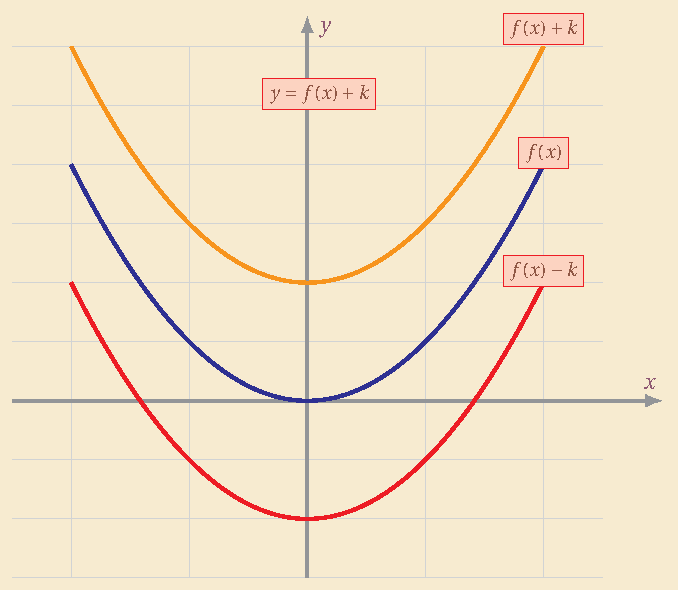
\includegraphics[scale=0.6]
{../mathbook-caos-calculo/images/ej-1-3-3.pdf}%
\caption{Suma de una funci\'{o}n con una constante}%
\label{traslacionejey1}%
\end{figure}


Por su parte, el producto de una funci\'{o}n real $f$ por una funci\'{o}n
constante positiva y diferente de $1$ produce una
\index{Funci\'{o}n!Gr\'{a}fica de una --!Contracci\'{o}n |textit}%
\index{Funci\'{o}n!Gr\'{a}fica de una --!Dilataci\'{o}n|textit}
contracci\'{o}n o una dilataci\'{o}n (\textquotedblleft estiramiento
vertical\textquotedblright) de la gr\'{a}fica de $f$. El producto de $f$ por
$-1$ produce, por su parte una reflexi\'{o}n%
\index{Funci\'{o}n!Gr\'{a}fica de una --!Reflexi\'{o}n|textit}
de la gr\'{a}fica de $f$ con relaci\'{o}n al eje $x$ (ver figura
\ref{contradilata1}).%

\begin{figure}[H]
\centering
\includegraphics[scale=0.8]%
{../mathbook-caos-calculo/images/ej-1-3-4.pdf}%
\caption{Producto de una funci\'{o}n por una constante}%
\label{contradilata1}%
\end{figure}



\paragraph{}

Dado un conjunto no vac\'{\i}o $A$, el conjunto de todas las funciones reales
con dominio $A$ puede dotarse de una \textquotedblleft estructura
algebraica\textquotedblright, definiendo ope\-raciones entre sus elementos. Si
$\rz^{A}$ es el conjunto de tales funciones, entonces para $f,g\in\rz^{A}$, es
claro que $f+g$ y $fg$ son elementos de
\index{a@$(\rz^{A},+,\cdot)$|textbf}%
$\rz^{A}$. La estructura algebraica $(\rz^{A},+,\cdot)$ goza de algunas
propiedades similares a la de la estructura aditivo-multiplicativa de los
reales, algo que no es de extra\~{n}ar, dada la forma como fueron definidas
las operaciones entre funciones.

\begin{theorem}
Sean $f,g,h\in\rz^{A}$. Entonces:

\begin{description}
\item[Leyes asociativas:] $(f+g)+h=f+(g+h)$ y $(fg)h=f(gh)$.

\item[Leyes conmutativas:] $f+g=g+f$ y $fg=gf$.

\item[Existencia de neutros:] Las funciones constantes $O,L\in\rz^{A}$
definidas por
\begin{align}
O(x)  &  =0\\
L(x)  &  =1
\end{align}
satisfacen $f+O=O+f=f$ y $fL=Lf=f$

\item[Existencia de inversos aditivos:] Si $-f=(-1)f$, entonces:
\[
f+(-f)=-f+f=O.
\]

\end{description}
\end{theorem}

\begin{proof}
Las propiedades anteriores son consecuencia de las correspondientes en la
estructura $(\rz,+,\cdot)$. Como ilustraci\'{o}n probemos la asociatividad de
la suma.\newline Para $x\in A$, se tiene que
\begin{align*}
((f+g)+h)(x)  &  =(f+g)(x)+h(x)\\
&  =(f(x)+g(x))+h(x)\\
&  =f(x)+(g(x)+h(x))\\
&  =f(x)+((g+h)(x))\\
&  =(f+(g+h))(x)
\end{align*}
de donde se tiene $(f+g)+h=f+(g+h)$.
\end{proof}

La funci\'{o}n $O$ del teorema anterior es la funci\'{o}n id\'{e}nticamente%
\index{Funci\'{o}n!-- identicamente nula}
nula. Las propiedades listadas en el teorema anterior caracterizan a la
estructura $(\rz^{A},+\cdot)$ como un anillo conmutativo con unidad . Nos
referiremos a el como el \textquotedblleft anillo de funciones reales sobre
$A$\textquotedblright.

\section{Composici\'{o}n de funciones}

Adem\'{a}s de la combinaci\'{o}n de funciones reales (o de funciones con rango
con alguna estructura algebraica) mediante operaciones como la adici\'{o}n y
multiplicaci\'{o}n, podemos tambi\'{e}n \textquotedblleft
conectar\textquotedblright, empalmar o \textquotedblleft
componer\textquotedblright\ dos funciones tales que las im\'{a}genes de una
pertenezcan al dominio de la otra. Para fijar ideas, consideremos funciones
$f$ y $g$ y un elemento $x\in\operatorname*{Dom}(f)$, tal que $f(x)\in
\operatorname*{Dom}(g)$, de modo que $g(f(x))$ est\'{a} definida. Podemos
entonces considerar $g(f(x))$, resultado de las acciones consecutivas de $f$ y
$g$ sobre $x$, como el resultado de una funci\'{o}n a la que denominaremos la
\index{Funci\'{o}n!-- compuesta}%
compuesta de $f$ con $g$. Tal funci\'{o}n ser\'{a} denotada por $g\circ f$. El
esquema siguiente ilustra la situaci\'{o}n.
\[
x\longrightarrow\framebox[2cm]{$f$}\longmapsto f(x)\longmapsto
\framebox[2cm]{$g$}\longmapsto(g\circ f)(x)=g(f(x))
\]
Formalizamos la definici\'{o}n de la operaci\'{o}n composici\'{o}n de funciones.

\begin{definition}
Sean $f:A\longrightarrow B,\ g:C\longrightarrow D$, funciones tales que
$\operatorname*{Ran}(f)\cap\operatorname*{Dom}(g)\neq\emptyset$. La
funci\'{o}n compuesta de $f$ con $g$ es la funci\'{o}n definida por:
\[%
\begin{array}
[c]{cccc}%
\label{compuesta}g\circ f: & \{x\in\operatorname*{Dom}(f)\mid f(x)\in
\operatorname*{Dom}(g)\} & \longrightarrow & D\\
& x & \longmapsto & g(f(x))
\end{array}
\]

\end{definition}

En la definici\'{o}n
\index{Dominio!-- de la funci\'{o}n compuesta}%
anterior, $f$ es denominada la
\index{Funci\'{o}n!-- interna}%
funci\'{o}n interna de la compuesta $g\circ f$. Por supuesto, $g$ es la
funci\'{o}n%
\index{Funci\'{o}n!-- externa}
externa de la compuesta $g\circ f$. N\'{o}tese que si, en particular,
$\operatorname*{Ran}(f)\subseteq\operatorname*{Dom}(g)=C$, entonces
$\operatorname*{Dom}(g\circ f)=\operatorname*{Dom}(f)$. En general, sin
embargo, la composici\'{o}n implica trabajar con restricciones de las
funciones que se componen.

\begin{example}
Debe tenerse cautela al determinar el dominio de una compuesta. Por ejemplo si
$f(x)=x^{2}$ y $g(x)=\sqrt{x}$, para $x$ en el dominio de $g$ se tiene que%
\[
f(g(x))=f(\sqrt{x})=(\sqrt{x})^{2}=x,
\]
lo que podr\'{\i}a llevar a pensar que la compuesta $f\circ g$ es la
funci\'{o}n identidad definida por $I_{\rz}(x)=x$, cuyo dominio es $\rz$. Es
claro, sin embargo, que la compuesta es solo la restricci\'{o}n de la
identidad al conjunto de los reales no negativos, restricci\'{o}n impuesta por
el dominio de la funci\'{o}n interna $g$.
\end{example}

\begin{example}
Por otra parte, se tiene que
\[
(g\circ f)(x)=\sqrt{x^{2}}=|x|,\mbox{ \ para todo real \ }x.
\]

\end{example}

\begin{remark}
N\'{o}tese que al componer dos funciones, realmente se consideran
restricciones adecuadas de las mismas. As\'{\i}, la compuesta de $f$ con $g$
coincide con la de las restricciones
\[
f|_{\{x\in\operatorname*{Dom}(f)\mid f(x)\in\operatorname*{Dom}(g)\}}%
,g|_{\operatorname*{Ran}(f)\cap\operatorname*{Dom}(g)}.
\]
Por lo que, sin p\'{e}rdida de generalidad, podemos suponer en la
definici\'{o}n de compuesta que $f$ y $g$ son funciones
\[
f:X\longrightarrow Y,\ \ g:Y\longrightarrow Z
\]
y que la compuesta de $f$ con $g$ est\'{a} dada por
\[%
\begin{array}
[c]{cccc}%
g\circ f: & X & \longrightarrow & Z\\
& x & \longmapsto & g(f(x))
\end{array}
\]

\end{remark}

\paragraph{}

Para un conjunto cualquiera no vac\'{\i}o $X$, denotamos por $I_{X}$, a la
funci\'{o}n identidad%
\index{Funci\'{o}n!-- identidad}
en $X$, definida por
\begin{equation}
I_{X}(x)=x,\mbox{ \ para todo \ }x\in X \label{identidadX}%
\end{equation}
El siguiente teorema muestra que la composici\'{o}n es una operaci\'{o}n
asociativa y que existen elementos neutros \textquotedblleft
unilaterales\textquotedblright\ para la misma operaci\'{o}n.

\begin{theorem}
\label{compuestaasociativa} Sean $f:X\longrightarrow Y,g:Y\longrightarrow
Z,h:Z\longrightarrow W$ funciones. Entonces:
\begin{equation}
h\circ(g\circ f)=(h\circ g)\circ f \label{asociacompuesta}%
\end{equation}%
\begin{equation}
f\circ I_{X}=I_{Y}\circ f=f \label{neutrocompuesta}%
\end{equation}

\end{theorem}

\begin{proof}
\hfil


\begin{enumerate}
\item Sea $x\in X$, entonces:
\begin{align*}
(h\circ(g\circ f))(x)  &  =h((g\circ f)(x))\\
&  =h(g(f(x))\\
&  =(h\circ g)(f(x))\\
&  =((h\circ g)\circ f)(x)
\end{align*}
Se tiene as\'{\i} que $h\circ(g\circ f)=(h\circ g)\circ f$.

\item Para $x\in X$ tenemos que
\begin{align*}
(f\circ I_{X})(x)  &  =f(I_{X}(x))\\
&  =f(x)\\
&  =I_{Y}(f(x))\\
&  =(I_{Y}\circ f)(x)
\end{align*}
lo que demuestra (\ref{neutrocompuesta}).
\end{enumerate}
\end{proof}

La ecuaci\'{o}n \ref{asociacompuesta} establece la asociatividad de la
composici\'{o}n. Por su parte (\ref{neutrocompuesta}) nos dice que $I_{X}$ es
un neutro \textquotedblleft a derecha\textquotedblright\ para funciones de $X$
a $Y$ y que $I_{Y}$ es un neutro \textquotedblleft a
izquierda\textquotedblright\ para las mismas funciones.

\begin{example}
Consideremos la funci\'{o}n real $f$ definida por
\[
f(x)=x^{2},\mbox{ \ para todo \ }x\in\rz.
\]
Claramente, $f$ no es una funci\'{o}n uno-a-uno, pues para todo real positivo
$y$, la ecuaci\'{o}n $f(x)=x^{2}=y$ tiene dos soluciones distintas $-\sqrt{y}$
y $\sqrt{y}$. Si consideramos la restricci\'{o}n $f|_{\left[  0,+\infty
\right[  }$, \'{e}sta resulta, en cambio, ser inyectiva. La relaci\'{o}n
inversa
\[
g=\{(y,x)\mid(x,y)\in{f\mid}_{\left[  0,+\infty\right[  }\}=\{(y,\sqrt{y})\mid
y\in\left[  0,+\infty\right[  \}
\]
es entonces una funci\'{o}n, pues cada real no negativo $y$ tiene una
\'{u}nica im\'{a}gen. Tal funci\'{o}n es entonces
\[%
\begin{array}
[c]{cccc}%
g: & \left[  0,+\infty\right[  & \longrightarrow & \left[  0,+\infty\right[ \\
& x & \longmapsto & \sqrt{x}%
\end{array}
\]
\textquestiondown Cu\'{a}l es la funci\'{o}n compuesta de la restricci\'{o}n
de $f$ considerada con la funci\'{o}n $g$?\newline Para un real no negativo
$x$ (es decir, en el dominio de la restricci\'{o}n) se tiene:
\begin{align*}
(g\circ f)(x)  &  =g(f(x))\\
&  =g(x^{2})\\
&  =\sqrt{x^{2}}\\
&  =|x|\\
&  =x\\
&  ={I}_{\left[  0,+\infty\right[  }(x)
\end{align*}
De manera similar, se tiene para un $x$ en el dominio de $g$ :
\begin{align*}
(f\circ g)(x)  &  =f(g(x))\\
&  =f(\sqrt{x})\\
&  =\left(  \sqrt{x}\right)  ^{2}\\
&  =x\\
&  =I_{[0,+\infty)}(x);
\end{align*}
Tenemos as\'{\i} que
\[
(g\circ f)(x)=(f\circ g)(x)=I(x),\mbox{ \ para todo \ }x\in\left[
0,+\infty\right[  ,
\]
es decir
\[
f\circ g=g\circ f=I_{\left[  0,+\infty\right[  }%
\]
en el conjunto . Decimos entonces que $g$ es una inversa de $f$ en el conjunto
$\left[  0,+\infty\right[  $. A continuaci\'{o}n formalizamos las definiciones
de funci\'{o}n invertible y de funci\'{o}n inversa.
\end{example}

\begin{definition}
\label{relacioninversa} Sea $R$ una relaci\'{o}n, la
\index{Relaci\'{o}n!-- inversa}%
relaci\'{o}n inversa (o dual) de $R$ es la relaci\'{o}n
\begin{equation}
R^{\ast}=\{(x,y)\mid(y,x)\in R\} \label{ecrelacioninversa}%
\end{equation}
Una funci\'{o}n $f:A\longrightarrow B$ se denomina invertible%
\index{Funci\'{o}n!-- invertible}
si, y solo si la relaci\'{o}n inversa $f^{\ast}$ es tambi\'{e}n una funci\'{o}n.
\end{definition}

Se siguen de la definici\'{o}n

\begin{theorem}
\label{caracterizainversa} Sea $f:A\longrightarrow B$ una funci\'{o}n. Son equivalentes:

\begin{enumerate}
\item $f$ es invertible.

\item $f$ es uno-a-uno.%
\index{Funci\'{o}n!-- inyectiva}%


\item Existe una funci\'{o}n $g:\operatorname*{Ran}(f)\longrightarrow A$, tal
que
\begin{equation}
g\circ f=I_{A},f\circ g=I_{\operatorname*{Ran}(f)}%
\end{equation}

\end{enumerate}
\end{theorem}

\begin{proof}
\hfill

\begin{enumerate}
\item Supongamos que $f$ es invertible y demostremos que es uno-a-uno.
Te\-nemos que $f^{\ast}=\{(x,y)\mid(y,x)\in f\}$ es una funci\'{o}n, por lo
que para todo $x\in\operatorname*{Ran}(f)$, existe una \'{u}nica im\'{a}gen
$y=f^{\ast}(x)$; es decir existe un \'{u}nico $y\in A$ tal que $f(y)=x$. Esto
muestra que $f$ es uno-a-uno.

\item Rec\'{\i}procamente, supongamos que $f$ es uno-a-uno y demostremos ahora
que la relaci\'{o}n inversa $f^{\ast}$ es una funci\'{o}n. Puesto que el
dominio de $f^{\ast}$ es el rango de $f$, consideremos $x\in
\operatorname*{Ran}(f)$. Por la inyectividad de $f$ se sigue que $x$ tiene una
\'{u}nica preim\'{a}gen $y$, o sea $x=f(y)$; as\'{\i}, existe un \'{u}nico
$y\in A$ tal que $(x,y)\in f^{\ast}$. Tenemos as\'{\i} que cada elemento del
dominio de $f^{\ast}$ tiene im\'{a}gen \'{u}nica y, por tanto, $f^{\ast}$ es
una funci\'{o}n. Tomando $g=f^{\ast}$, entonces para $x\in A$ se tiene
\begin{align*}
(x,f(x))\in f  &  \Longrightarrow(f(x),x)\in f^{\ast}\\
&  \Longrightarrow f^{\ast}(f(x))=x\\
&  \Longrightarrow(g\circ f)(x)=I_{A}(x)
\end{align*}
De manera similar, para $x\in\operatorname*{Ran}(f)$, existe $y\in A$ tal que
$x=f(y)$, por lo que $(x,y)\in f^{\ast}$. Se tiene entonces
\begin{align*}
x  &  =f(y)\\
&  =f(f^{\ast}(x))\\
&  =f(g(x))
\end{align*}
de donde se sigue que $f\circ g=I_{\operatorname*{Ran}(f)}$.

\item Para completar la demostraci\'{o}n consideremos ahora que existe una
funci\'{o}n $g$ con las condiciones dadas en el item $3$ del teorema.
Mostremos entonces que la relaci\'{o}n inversa $f^{\ast}$, como conjunto de
pares ordenados, es la misma funci\'{o}n $g$. Consideremos un par ordenado
$(x,y)$. Entonces:
\begin{align*}
(x,y)\in g  &  \Longrightarrow y=g(x)\\
&  \Longrightarrow f(y)=f(g(x))=x\\
&  \Longrightarrow(y,x)\in f\\
&  \Longrightarrow(x,y)\in f^{\ast}%
\end{align*}
Tambi\'{e}n se tiene
\begin{align*}
(x,y)\in f^{\ast}  &  \Longrightarrow(y,x)\in f\\
&  \Longrightarrow x=f(y)\\
&  \Longrightarrow g(x)=g(f(y))=y\\
&  \Longrightarrow(x,y)\in g
\end{align*}
Como $f^{\ast}=g$, se sigue que $f^{\ast}$ es una funci\'{o}n y que $f$ es invertible.
\end{enumerate}
\end{proof}

\paragraph{}

Si $f:A\longrightarrow B$ es una funci\'{o}n invertible, su inversa ser\'{a}
simbolizada por $f^{-1}$. Consideremos un punto $P(x,f(x))$ de la gr\'{a}fica
de $f$. Entonces se tiene que $Q(f(x),x)$ es un punto de la gr\'{a}fica de
$f^{-1}$. La figura \ref{simetriarectaidentidad}, muestra que tales puntos son
v\'{e}rtices opuestos de un cuadrado, con una de sus diagonales sobre la recta
de ecuaci\'{o}n $y=x$.%

\begin{figure}[H]
\centering
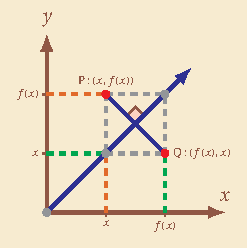
\includegraphics[scale=1.5]{../mathbook-caos-calculo/images/fig-1-5.pdf}%
\caption{Simetr\'{\i}a con relaci\'{o}n a $y=x$}%
\label{simetriarectaidentidad}%
\end{figure}



Es decir, tales puntos son sim\'{e}tricos respecto de dicha diagonal. Se sigue
que las gr\'{a}fica de $f^{-1}$ es la reflexi\'{o}n de la de $f$ con
relaci\'{o}n a la recta de ecuaci\'{o}n $y=x$ (ver figura \ref{finversa1}).

\begin{figure}[H]
\centering
\includegraphics[scale=1]%
{../mathbook-caos-calculo/images/fig-1-6.pdf}%
\caption{Funci\'{o}n inversa}%
\label{finversa1}%
\end{figure}


%TODO
\paragraph{}

El teorema \ref{caracterizainversa} establece que una funci\'{o}n es
invertible si, y solo si es 1-1. Sin embargo, una funci\'{o}n $f$ que no sea
inyectiva puede restringirse en su dominio\footnote{Si, por ejemplo, para
$y\in Ran(f)$ existen m\'{a}s de una \textquotedblleft pre-im\'{a}gen" de $y$,
podemos escoger una sola de estas y restringir el dominio de $f$ escogiendo
una sola preim\'{a}gen de cada elemento del rango, de forma que la
restricci\'{o}n resultante sea inyectiva} de manera tal que la restricci\'{o}n
escogida sea uno-a-uno. Tal restricci\'{o}n ser\'{a} entonces invertible y
diremos que su inversa es una \textquotedblleft inversa de $f$ en el dominio
de la restricci\'{o}n\textquotedblright.

\section{Sucesiones y series de n\'{u}meros reales}

Un caso particular de funciones reales es de inter\'{e}s en esta secci\'{o}n.
Informalmente hablando, una
\index{Sucesi\'{o}n|textbf}%
sucesi\'{o}n en un conjunto cualquiera no vac\'{\i}o $A$ es una funci\'{o}n
con valores sobre ese conjunto y cuya variable recorre un conjunto infinito de
n\'{u}meros enteros no negativos consecutivos. Precisando el concepto, si
$n_{o}$ es un entero no negativo (un n\'{u}mero natural) y $J=\{n\in\nz\mid
n\geq n_{0}\}$, entonces una funci\'{o}n
\[
\alpha:J\longrightarrow A
\]
se denomina una sucesi\'{o}n en o sobre el conjunto $A$. Si $A=\rz$, decimos
que $\alpha$ es una sucesi\'{o}n de n\'{u}meros reales o, m\'{a}s brevemente,
una sucesi\'{o}n real.

\begin{definition}
Sean $n_{0}\in\nz_{0}$. Una funci\'{o}n
\[
\alpha:J=\{n\in\nz\mid n\geq n_{0}\}\longrightarrow\rz
\]
es denominada sucesi\'{o}n real.
\end{definition}

En las condiciones de la definici\'{o}n anterior, la sucesi\'{o}n $\alpha$
ser\'{a} descrita generalmente por sus im\'{a}genes. En ese sentido, la
notaci\'{o}n $\{\alpha(n)\}_{n=n_{0}}^{\infty}$ o $\{\alpha(n)\}_{n\in J}$ se
utilizar\'{a} para referirse a la sucesi\'{o}n $\alpha$. El rango de la
sucesi\'{o}n, es decir el conjunto
\[
\{\alpha(n_{0}),\alpha(n_{0}+1),\alpha(n_{0}+2),\dots\},
\]
puede ser un conjunto finito o infinito. En todo caso, si bien formalmente
hablando la sucesi\'{o}n es la funci\'{o}n $\alpha$, nuestro inter\'{e}s
estar\'{a} centrado en dicho rango, puesto de relieve por la notaci\'{o}n. Se
acostumbra a decir que cada im\'{a}gen $\alpha(n)$ es un t\'{e}rmino de la
sucesi\'{o}n $\alpha$.

\begin{example}
La sucesi\'{o}n real $\alpha:\nz\longrightarrow\rz$, definida por
\[
\alpha(n)=\frac{1}{n}%
\]
ser\'{a} notada como
\[
\left\{  \frac{1}{n}\right\}  _{n\in\nz}.
\]
As\'{\i}, la sucesi\'{o}n considerada toma los valores reales
\[
\left\{  1,\frac{1}{2},\frac{1}{3},\frac{1}{4},\dots\right\}  .
\]
N\'{o}tese que el mismo conjunto de valores es recorrido por las sucesiones
\[
\left\{  \frac{1}{n+1}\right\}  _{n\in\nz_{0}},
\]%
\[
\left\{  \frac{1}{n-1}\right\}  _{n=2}^{\infty},
\]%
\[
\left\{  \frac{1}{n-5}\right\}  _{n=6}^{\infty},
\]
por lo que las sucesiones consideradas podr\'{\i}an considerarse iguales, en
el sentido que producen los mismos valores en el \textquotedblleft mismo
orden\textquotedblright.
\end{example}

\paragraph{}

Precisando la idea del ejemplo anterior, dada una sucesi\'{o}n cualquiera
$\{\alpha(n)\}_{n=n_{0}}^{\infty}$, la funci\'{o}n

\begin{center}
\begin{tabular}
[c]{cccc}%
$f:$ & $\nz$ & $\longrightarrow$ & $J=\{n\in\gz\mid n\geq n_{0}\}$\\
& $1$ & $\longmapsto$ & $n_{0}$\\
& $2$ & $\longmapsto$ & $n_{0}+1$\\
& $3$ & $\longmapsto$ & $n_{0}+2$\\
& $\Vdots$ & $\Vdots$ & $\Vdots$\\
& $n$ & $\longmapsto$ & $n_{0}+(n-1)$\\
&  &  &
\end{tabular}
\end{center}


es biyectiva y para cada natural $n$ se tiene que
\begin{center}
\begin{tabular}[c]{ccc}
$(\alpha\circ f)(1)$  & $ = $     &$\alpha(n_{0})$\\
$(\alpha\circ f)(2)$  & $ = $     &$\alpha(n_{0}+1)$\\
$(\alpha\circ f)(3)$  & $ = $     &$\alpha(n_{0}+2)$\\
$\Vdots            $  & $\Vdots$  &$ \Vdots$
\end{tabular}
\end{center}
por lo que los valores de las sucesiones $\beta=\alpha\circ f$ y $\alpha$ son
los mismos, en el mismo orden. N\'{o}tese que el primer t\'{e}rmino de la
sucesi\'{o}n es $\alpha(n_{0})=\beta(1)$. As\'{\i}, sin p\'{e}rdida de
generalidad, podr\'{\i}amos considerar solo sucesiones cuyo dominio es el
conjunto de los n\'{u}meros naturales; es decir, sucesiones
\[
\{x_{n}\}_{n\in\nz},
\]
donde $x_{n}=\alpha(n)$ y $\alpha:\nz\longrightarrow\rz$ es una funci\'{o}n.

\begin{example}
Para la sucesi\'{o}n $\{\sqrt{n+5}\}_{n=4}^{\infty}$, la funci\'{o}n
\[
f:\nz\ni n\longmapsto n+3\in\{n\in\nz\mid n\geq4\}
\]
da origen a la sucesi\'{o}n
\[
\beta(n)=\sqrt{f(n)}=\sqrt{n+8},\mbox{ \ para todo \
}n\in\nz
\]
cuyo rango es el mismo de la sucesi\'{o}n dada.
\end{example}

\begin{example}
La sucesi\'{o}n $\{(-1)^{n}\}_{n\in\nz}$ tiene el rango finito $\{-1,1\}$
\end{example}

Dada una sucesi\'{o}n real $\{x_{n}\}_{n=n_{0}}^{\infty}$, para $n\geq n_{0}$,
definimos la $n-$\'{e}sima suma parcial
\index{Sucesi\'{o}n!a@$n-$\'{e}sima suma parcial}%
de la sucesi\'{o}n dada por
\begin{equation}
s_{n}=x_{n_{0}}+x_{n_{0}+1}+\dots+x_{n}=\sum_{i=n_{0}}^{n}x_{i}
\label{sumaparcial}%
\end{equation}
la sucesi\'{o}n de sumas parciales
\begin{equation}
\{s_{n}\}_{n=n_{0}}^{\infty}=\left\{  \sum_{i=n_{0}}^{n}x_{i}\right\}
_{n=n_{0}}^{\infty} \label{serie}%
\end{equation}
es denominada una serie real%
\index{Sucesi\'{o}n!Serie asociada a una --}%
. Diremos de ella que es la serie asociada a la sucesi\'{o}n dada.

\begin{example}
Las series asociadas a las sucesiones
\[
\{n+1\}_{n\in\nz},\ \left\{  \frac{1}{n}\right\}  _{n\in\nz}%
\ \mbox{ \ y \ }\{(-1)^{n}\}_{n\in\nz_{0}}%
\]
son, respectivamente
\begin{align*}
\left\{  \sum_{i=1}^{n}(i+1)\right\}  _{n\in\nz}  &
=\{2,2+3,2+3+4,2+3+4+5,\dots\}\\
&  =\{2,5,9,14,\dots\}\\
\left\{  \sum_{i=1}^{n}\frac{1}{i}\right\}  _{n\in\nz}  &  =\left\{
1,1+\frac{1}{2},1+\frac{1}{2}+\frac{1}{3},1+\frac{1}{2}+\frac{1}{3}+\frac
{1}{4},\dots\right\} \\
&  =\left\{  1,\frac{3}{2},\frac{11}{6},\frac{25}{12},\dots\right\} \\
\left\{  \sum_{i=0}^{n}(-1)^{i}\right\}  _{n\in\nz_{0}}  &
=\{1,1+(-1),1+(-1)+1,1+(-1)+1+(-1),\dots\}\\
&  =\{1,0,1,0,\dots\}
\end{align*}

\end{example}

\begin{example}
Para un real fijo $x\neq0$ la sucesi\'{o}n $\{x^{n}\}_{n\in\nz_{0}}$, da
origen a la denominada serie geom\'{e}trica
\begin{equation}
\left\{  \sum_{i=n}^{n}x^{i}\right\}  _{n\in\nz_{0}}=\{1,1+x,1+x+x^{2},\dots\}
\end{equation}
Para $x=0$, la serie geom\'{e}trica est\'{a} determinada por la sucesi\'{o}n
\[
\alpha(n)=%
\begin{cases}
1, & \text{si $n=0$}\\
0^{n}=0, & \text{ si $n>0$}%
\end{cases}
\]
Es decir, el recorrido de la serie geom\'{e}trica es
\[
\{1,1+0,1+0+0,\dots\}.
\]

\end{example}

\paragraph{}

Se acostumbra a escribir
\[
\sum_{n=n_{0}}^{\infty}x_{n}%
\]
para la serie
\[
\left\{  \sum_{i=n_{0}}^{n}x_{i}\right\}  _{n=n_{0}}^{\infty}%
\]


%%%%%%%%%%%%%%%%%%%%%%%%%%%%%%%%%%%%%%%%%%%%%%%%%%%%%%%%%%%%%%%%%%%%%%%%%%%%%%%%%


\section{Ejercicios resueltos}

\begin{example}
Sean $A=\left\{  1,3,-2,5\right\}  $ y $B=\left\{  0,3,2,-1,4\right\}  $ y las
relaciones $R_{k}:A\longrightarrow B,$ $k=1,\ldots,5,$definidas por:
\begin{align*}
R_{1}  &  =\left\{  \left(  1,2\right)  ,\left(  3,3\right)  ,\left(
-2,4\right)  \right\} \\
R_{2}  &  =\left\{  \left(  1,2\right)  ,\left(  3,0\right)  ,\left(
-2,-1\right)  ,\left(  5,4\right)  \right\} \\
R_{3}  &  =\left\{  \left(  3,4\right)  ,\left(  -2,4\right)  ,\left(
1,4\right)  ,\left(  5,4\right)  \right\} \\
R_{4}  &  =\left\{  \left(  -2,0\right)  ,\left(  5,3\right)  ,\left(
3,-1\right)  ,\left(  1,2\right)  ,\left(  3,4\right)  \right\} \\
R_{5}  &  =A\times B
\end{align*}
Determine para cada caso el dominio y el rango, e indique si es funci\'{o}n.
\end{example}

\begin{sol}
El dominio y el rango en cada caso vienen dados por
\[%
\begin{array}
[c]{lll}%
\operatorname*{Dom}\left(  R_{1}\right)  =\left\{  1,3,-2\right\}  &  &
\operatorname*{Ran}\left(  R_{1}\right)  =\left\{  2,3,4\right\} \\
\operatorname*{Dom}\left(  R_{2}\right)  =A &  & \operatorname*{Ran}\left(
R_{2}\right)  =\left\{  4\right\} \\
\operatorname*{Dom}\left(  R_{3}\right)  =A &  & \operatorname*{Ran}\left(
R_{3}\right)  =\left\{  2,0,-1,4\right\} \\
\operatorname*{Dom}\left(  R_{4}\right)  =A &  & \operatorname*{Ran}\left(
R_{4}\right)  =B\\
\operatorname*{Dom}\left(  R_{5}\right)  =A &  & \operatorname*{Ran}\left(
R_{5}\right)  =B
\end{array}
\]
Analizando esta informaci\'{o}n se observa que s\'{o}lo las relaciones $R_{2}$
y $R_{3}$ son funciones, ya que tienen como dominio a $A$ y cada elemento del
dominio tiene imagen \'{u}nica.

$R_{1}$ no es una funci\'{o}n por que $\operatorname*{Dom}\left(
R_{1}\right)  \neq A.$ $R_{4}$ y $R_{5}$ no son funciones porque existen
elementos del dominio que no tienen una \'{u}nica imagen. Por ejemplo $\left(
3,-1\right)  $ y $\left(  3,4\right)  $ en $R_{4},$ y $\left(  1,0\right)  $ y
$\left(  1,3\right)  $ en $R_{5}$.
\end{sol}

\begin{example}
Consideremos las funciones $f$ y $g$ definidas a continuaci\'{o}n:
\[%
\begin{array}
[c]{ccccccccc}%
f: & \rz & \longrightarrow & \rz & \,\,\, & g: & \rz & \longrightarrow & \rz\\
& x & \longmapsto & x^{2}+x+1 & \,\,\, &  & x & \longmapsto & 2x+3
\end{array}
.
\]
Determine para cada una si son uno a uno o sobreyectiva. Adem\'{a}s calcule el
Rango de las funciones.
\end{example}

\begin{sol}
Tenemos que $f(x)=x^{2}+x+1$ para todo real $x$. $f$ no es sobreyectiva, pues
dado un real $y$, la ecuaci\'{o}n cuadr\'{a}tica
\[
x^{2}+x+1=y,\ \mbox{ \ es decir, \ }x^{2}+x+(1-y)=0
\]
solo tiene soluciones reales si, y solo si el discriminante $1-4(1)(1-y)=4y-3$
es no negativo. Ahora
\[
4y-3\geq0\Longleftrightarrow y\geq\frac{3}{4},
\]
lo que muestra que $\operatorname*{Ran}(f)=\left[  \frac{3}{4},\infty\right[
$. As\'{\i}, por ejemplo, no existe un real $x$ tal que $f(x)=x^{2}+x+1=0$.
Por otra parte para $y>\frac{3}{4}$, la ecuaci\'{o}n cuadr\'{a}tica
considerada tiene dos soluciones distintas, por lo que para un tal valor de
$y$ existen dos elementos distintos del dominio cuya im\'{a}gen es la misma,
$y$. Considere, como ilustraci\'{o}n, $y=1$; se tiene entonces
\[
f(x)=x^{2}+x+1=1\Longleftrightarrow x=0\vee x=-1.
\]
Esto muestra que $f$ no es uno-a-uno.

Para $g$ tenemos que dado un real $y$, la ecuaci\'{o}n lineal
\[
g(x)=2x+3=y
\]
tiene siempre soluci\'{o}n \'{u}nica $x=\frac{y-3}{2}$. La existencia de
soluci\'{o}n muestra que la funci\'{o}n es sobre; es decir
$\operatorname*{Ran}(g)=\rz$. El que la soluci\'{o}n sea \'{u}nica indica que
$g$ es uno-a-uno. As\'{\i}, $g$ es una funci\'{o}n biyectiva.
\end{sol}

\begin{example}
Determine el v\'{e}rtice y el rango de $f(x)=x^{2}+3x+2$. Analice la
gr\'{a}fica de la funci\'{o}n.
\end{example}

\begin{sol}
La funci\'{o}n cuadr\'{a}tica dada por $f(x)=x^{2}+3x+2$, tiene una
gr\'{a}fica con v\'{e}rtice en
\[
V\left(  -\frac{3}{2},\frac{8-9}{4}\right)  =V\left(  -\frac{3}{2},-\frac
{1}{4}\right)  ,
\]
por lo que su rango es $\left[  -\frac{1}{4},+\infty\right[  $. El eje de
simetr\'{\i}a es la recta de ecuaci\'{o}n $x=-\frac{3}{2}$. Para trazar un
esbozo a mano de la gr\'{a}fica podemos considerar algunos valores de $x$
menores que $-\frac{3}{2}$; puntos sim\'{e}tricos a cada punto con abscisa $x$
tendr\'{a}n abscisas con valor igual al de $x$ m\'{a}s su distancia al eje de
simetr\'{\i}a. Las ordenadas de puntos sim\'{e}tricos son las mismas. Una
tabla de algunos valores de $x$ e $y$ para la gr\'{a}fica se muestra a
continuaci\'{o}n.
\[%
\begin{tabular}
[c]{|c||c|c|c|c|c|}\hline
$x$ & $-3/2$ & $-5/2,-1/2$ & $-7/2,1/2$ & $-9/2,3/2$ & $-11/2,5/2$\\\hline
$y=f(x)$ & $-\frac{1}{4}$ & $3/4$ & $15/4$ & $35/4$ & $63/4$\\\hline
\end{tabular}
\ \ \ \ \ \ \
\]
Una gr\'{a}fica con computador se muestra en la figura \ref{ejemplopa1}%
\newline%

\begin{figure}[H]
\centering
\includegraphics[scale=0.7]%
{../mathbook-caos-calculo/images/fig-1-7.pdf}%
\caption{Gr\'{a}fica de $f(x)=x^{2}+2x+3$}%
\label{ejemplopa1}%
\end{figure}


\end{sol}
%TODO 
\begin{example}
Sea la funci\'{o}n $y=f(x)=-3\sqrt{4-x^{2}}$

\begin{enumerate}
\item Hallar el dominio.

\item Calcular el rango.

\item Hallar $\dfrac{f\left(  x+h\right)  -f\left(  x\right)  }{h}$
\end{enumerate}
\end{example}

\begin{sol}
\begin{enumerate}
\item Para calcular el dominio de la funci\'{o}n $f,$ se tiene en cuenta que
\begin{align*}
\operatorname*{Dom}f  &  =\left\{  x\in\rz\mid4-x^{2}\geq0\right\} \\
&  =\left\{  x\in\rz\mid4\geq x^{2}\right\} \\
&  =\left\{  x\in\rz\mid\left\vert x\right\vert =\sqrt{x^{2}}\leq\sqrt
{4}\right\} \\
&  =\left\{  x\in\rz\mid-2\leq x\leq2\right\}  =\left[  -2,2\right]
\end{align*}


\item Para obtener el \ rango, observe que para $x\in\left[  -2,2\right]
,y=-3\sqrt{4-x^{2}}\leq0.$ Es decir
\begin{equation}
y\in\left]  -\infty,0\right]  \label{a2}%
\end{equation}
Resolviendo la ecuaci\'{o}n anterior para $x$ se tiene
\begin{equation}
x=3\sqrt{4-\left(  \frac{y}{-3}\right)  ^{2}}\implies4-\frac{y^{2}}{9}%
\geq0\ \implies y\in\left[  -6,6\right]  \label{a3}%
\end{equation}
De $\left(  \ref{a2}\right)  $ y $\left(  \ref{a3}\right)  $ se tiene que el
rango de la funci\'{o}n es el intervalo $\left[  -6,0\right]  $

\item Ya que $f\left(  x\right)  =-3\sqrt{4-x^{2}},$ entonces $f\left(
x+h\right)  =-3\sqrt{4-\left(  x+h\right)  ^{2}}.$ Por lo cual,%
\[
\dfrac{f\left(  x+h\right)  -f\left(  x\right)  }{h}=-3\left(  \dfrac
{\sqrt{4-\left(  x+h\right)  ^{2}}-\sqrt{4-x^{2}}}{h}\right)  .
\]
Racionalizando el numerador se tiene que
\begin{align*}
\dfrac{f\left(  x+h\right)  -f\left(  x\right)  }{h}  &  =-3\left(
\dfrac{4-\left(  x+h\right)  ^{2}-\left(  4-x^{2}\right)  }{h\left(
\sqrt{4-\left(  x+h\right)  ^{2}}+\sqrt{4-x^{2}}\right)  }\right) \\
&  =-3\left(  \dfrac{-h\left(  2x+h\right)  }{h\left(  \sqrt{4-\left(
x+h\right)  ^{2}}+\sqrt{4-x^{2}}\right)  }\right) \\
&  =3\left(  \dfrac{2x+h}{\left(  \sqrt{4-\left(  x+h\right)  ^{2}}%
+\sqrt{4-x^{2}}\right)  }\right)  .
\end{align*}

\end{enumerate}
\end{sol}

\begin{example}
Sea $f(x)=\dfrac{x\sqrt{x^{2}-1}}{x^{2}-x-12}.$ Determine el dominio de la funci\'{o}n
\end{example}

\begin{sol}
Definamos $g\left(  x\right)  :=x\sqrt{x^{2}-1}$ y $h\left(  x\right)
:=x^{2}-x-12.$ Entonces $f\left(  x\right)  $ se puede expresar como el
cociente de estas dos funciones, es decir $f\left(  x\right)  =\dfrac{g\left(
x\right)  }{h\left(  x\right)  }$, por lo tanto%
\begin{equation}
\operatorname*{Dom}\left(  f\right)  =\operatorname*{Dom}\left(  g\right)
\cap\operatorname*{Dom}\left(  h\right)  -\left\{  x\mid h\left(  x\right)
=0\right\}  . \label{fgh}%
\end{equation}
A continuaci\'{o}n calculamos cada uno de los conjuntos dados en (\ref{fgh}).

\begin{enumerate}
\item Como $g\left(  x\right)  :=x\sqrt{x^{2}-1},$entonces
\begin{align*}
\operatorname*{Dom}g  &  =\left\{  x\in\rz\mid x^{2}-1\geq0\right\} \\
&  =\left\{  x\in\rz\mid x^{2}\geq1\right\} \\
&  =\left\{  x\in\rz\mid\left\vert x\right\vert =\sqrt{x^{2}}\geq1\right\} \\
&  =\left\{  x\in\rz\mid x\leq-1\vee1\leq x\right\} \\
&  =\left]  -\infty,-1\right]  \cup\left[  1,+\infty\right[
\end{align*}


\item Como $h\left(  x\right)  :=x^{2}-x-12$ es un polinomio, es claro que
$\operatorname*{Dom}h=\rz.$ Adem\'{a}s
\begin{align*}
\left\{  x\in\rz\mid x^{2}-x-12=0\right\}   &  =\left\{  x\in\rz\mid\left(
x+3\right)  \left(  x-4\right)  =0\right\} \\
&  =\left\{  -3,4\right\}
\end{align*}
En conclusi\'{o}n,
\begin{align*}
\operatorname*{Dom}\left(  f\right)   &  =\left(  -\infty,-1\right]
\cup\left[  1,+\infty\right)  \cap\rz-\left\{  -3,4\right\} \\
&  =\left(  -\infty,-1\right]  \cup\left[  1,+\infty\right)  -\left\{
-3,4\right\} \\
&  =\left]  -\infty,-3\right[  \cup\left]  -3,-1\right]  \cup\left[
1,4\right[  \cup\left]  4,+\infty\right[
\end{align*}

\end{enumerate}
\end{sol}

\begin{example}
Sean las funciones
\begin{align*}
f  &  =\left\{  \left(  1,2\right)  ,\left(  a,3\right)  ,\left(  -1,3\right)
,\left(  2,-2\right)  \right\} \\
g  &  =\left\{  \left(  1,4\right)  ,\left(  a,0\right)  ,\left(
-2,-1\right)  ,\left(  3,-3\right)  ,\left(  2,a\right)  \right\}
\end{align*}
Calcule el dominio y rango de $f$ y $g.$ Obtenga adem\'{a}s
$f+g,fg,f/g,g/f,g\circ f,f\circ g$.
\end{example}

\begin{sol}
En virtud a la definici\'{o}n de $f$ y $g$ se tiene que
\[%
\begin{array}
[c]{lll}%
\operatorname*{Dom}\left(  f\right)  =\left\{  1,a,-1,2\right\}  &  &
\operatorname*{Ran}\left(  f\right)  =\left\{  2,3,-2\right\} \\
\operatorname*{Dom}\left(  g\right)  =\left\{  1,a,-2,3,2\right\}  &  &
\operatorname*{Ran}\left(  g\right)  =\left\{  4,0,-1,-3,a\right\}  .
\end{array}
\]
En $\operatorname*{Dom}\left(  f\right)  \cap\operatorname*{Dom}\left(
g\right)  =\left\{  1,a,2\right\}  $ se definen las funciones%
\begin{align*}
f+g  &  =\left\{  \left(  1,6\right)  ,\left(  a,3\right)  ,\left(
2,a-2\right)  \right\} \\
fg  &  =\left\{  \left(  1,8\right)  ,\left(  a,0\right)  ,\left(
2,-2a\right)  \right\}
\end{align*}
y en los conjuntos
\begin{align*}
\operatorname*{Dom}\left(  f\right)  \cap\operatorname*{Dom}\left(  g\right)
-\left\{  x\in\operatorname*{Dom}\left(  g\right)  \mid g\left(  x\right)
=0\right\}   &  =\left\{  1,2\right\} \\
\operatorname*{Dom}\left(  f\right)  \cap\operatorname*{Dom}\left(  g\right)
-\left\{  x\in\operatorname*{Dom}\left(  f\right)  \mid f\left(  x\right)
=0\right\}   &  =\left\{  1,a,2\right\}
\end{align*}
se definen respectivamente%
\begin{align*}
f/g  &  =\left\{  \left(  1,\frac{1}{2}\right)  ,\left(  2,-\frac{2}%
{a}\right)  \right\} \\
g/f  &  =\left\{  \left(  1,2\right)  ,\left(  a,0\right)  ,\left(
2,-\frac{a}{2}\right)  \right\}  .
\end{align*}
Ya que $\operatorname*{Ran}\left(  g\right)  \cap\operatorname*{Dom}\left(
f\right)  =\left\{  -1\right\}  \neq\emptyset$, y $\operatorname*{Ran}\left(
f\right)  \cap\operatorname*{Dom}\left(  g\right)  =\left\{  2,3,-2\right\}
\neq\emptyset,$ entonces $f\circ g$ y $g\circ f$ est\'{a}n bien definidas, y
dadas por%
\begin{align*}
f\circ g  &  =\left\{  \left(  2,-3\right)  \right\} \\
g\circ f  &  =\left\{  \left(  1,a\right)  ,\left(  a,-3\right)  ,\left(
-1,-3\right)  ,\left(  2,-1\right)  \right\}  .
\end{align*}
De lo anterior es obvio que%
\begin{align*}
\operatorname*{Dom}\left(  f\circ g\right)   &  =\{x\in\operatorname*{Dom}%
(g)\mid g(x)\in\operatorname*{Dom}(f)\}=\left\{  2\right\} \\
\operatorname*{Dom}\left(  g\circ f\right)   &  =\{x\in\operatorname*{Dom}%
(f)\mid f(x)\in\operatorname*{Dom}(g)\}=\left\{  1,a,-1,2\right\}  .
\end{align*}

\end{sol}

\begin{example}
Sea $f\left(  x\right)  =\dfrac{x^{2}+1}{x^{2}-3}$, y $g\left(  x\right)
=-\sqrt{x^{2}-1}.$ De una formula para $h(x)=\left(  f\circ g\right)  \left(
x\right)  ,$ y calcule el dominio de $f\circ g$.
\end{example}

\begin{sol}
Si consideramos la compuesta entre $f$ y $g$ se tiene que
\begin{align*}
\left(  f\circ g\right)  \left(  x\right)   &  =\dfrac{\left(  -\sqrt{x^{2}%
-1}\right)  ^{2}+1}{\left(  -\sqrt{x^{2}-1}\right)  ^{2}-3}\overset{%
%TCIMACRO{\QATOP{x\in\operatorname*{Dom}g}{\downarrow}}%
%BeginExpansion
\genfrac{}{}{0pt}{}{x\in\operatorname*{Dom}g}{\downarrow}%
%EndExpansion
}{=}\frac{x^{2}-1+1}{x^{2}-1-3}\\
&  =\frac{x^{2}}{x^{2}-4}.
\end{align*}
Como
\[%
\begin{array}
[c]{cccc}%
g: & \operatorname*{Dom}(g)=\left]  -\infty,-1\right]  \cup\left[
1,+\infty\right[  & \longrightarrow & \rz^{-}\cup\left\{  0\right\} \\
\vspace{-0.2cm} &  &  & \\
& x & \longmapsto & -\sqrt{x^{2}-1}%
\end{array}
\]
y
\[%
\begin{array}
[c]{cccc}%
f: & \operatorname*{Dom}(f)=\rz-\left\{  \pm\sqrt{3}\right\}  &
\longrightarrow & \left]  -\infty,-\frac{1}{3}\right]  \cup\left]
1,+\infty\right[ \\
\vspace{-0.2cm} &  &  & \\
& x & \longmapsto & \dfrac{x^{2}+1}{x^{2}-3},
\end{array}
\]
es claro que la compuesta $f\circ g$ existe, y%
\[
\operatorname*{Dom}\left(  f\circ g\right)  =\{x\in\operatorname*{Dom}(g)\mid
g(x)\in\operatorname*{Dom}(f)\}.
\]
Si $x\in\operatorname*{Dom}\left(  f\circ g\right)  ,$ entonces

\begin{enumerate}
\item $x\in\left]  -\infty,-1\right]  \cup\left[  1,+\infty\right[  ,$ y

\item $g(x)\in\rz-\left\{  \pm\sqrt{3}\right\}  $
\end{enumerate}

De la segunda condici\'{o}n se tiene que $-\sqrt{x^{2}-1}\neq\pm\sqrt{3}.$ Es
claro que $-\sqrt{x^{2}-1}\neq+\sqrt{3},$ por lo tanto nos falta determinar el
conjunto%
\[
\left\{  x\in\operatorname*{Dom}(g)\mid-\sqrt{x^{2}-1}\neq-\sqrt{3}\right\}
=\left]  -\infty,-1\right]  \cup\left[  1,+\infty\right[  -\left\{
x\mid-\sqrt{x^{2}-1}=-\sqrt{3}\right\}
\]


pero $\left\{  x\mid-\sqrt{x^{2}-1}=-\sqrt{3}\right\}  =\left\{  \pm2\right\}
.$ Por lo tanto%

\begin{align*}
\operatorname*{Dom}\left(  f\circ g\right)   &  =\{x\in\operatorname*{Dom}%
(g)\mid g(x)\in\operatorname*{Dom}(f)\}\\
&  =\left(  -\infty,-1\right]  \cup\left[  1,+\infty\right)  -\left\{
\pm2\right\} \\
&  =\left]  -\infty,-2\right[  \cup\left]  -2,-1\right]  \cup\left[
1,2\right[  \cup\left]  2,+\infty\right[
\end{align*}

\end{sol}

\begin{example}
Consideremos las funciones reales definidas por
\[
f(x)=\sqrt{2x+9},\ \ g(x)=\sqrt{x^{2}-x-6}.
\]
Obtenga $\operatorname*{Dom}\left(  f\right)  ,\operatorname*{Dom}\left(
g\right)  ,f+g,fg,\frac{f}{g},\operatorname*{Dom}\left(  f+g\right)
,\operatorname*{Dom}\left(  fg\right)  ,\operatorname*{Dom}\left(  \frac{f}%
{g}\right)  .$
\end{example}

\begin{sol}
Se tiene que:
\begin{align*}
\operatorname*{Dom}(f)  &  =\{x\in\rz\mid2x+9\geq0\}\\
&  =\{x\in\rz\mid x\geq-9/2\}\\
&  =\left[  -\frac{9}{2},+\infty\right[ \\
\operatorname*{Dom}(g)  &  =\{x\in\rz\mid x^{2}-x-6=(x-3)(x+2)\geq0\}\\
&  =\left]  -\infty,-2\right]  \cup\left[  3,+\infty\right[
\end{align*}
Se tiene as\'{\i} que
\[
\operatorname*{Dom}(f)\cap\operatorname*{Dom}(g)=\left[  -\frac{9}%
{2},-2\right]  \cup\lbrack3,+\infty)
\]
conjunto sobre el cual est\'{a}n definidas las funciones
\begin{align*}
(f+g)(x)  &  =\sqrt{2x+9}+\sqrt{x^{2}-x-6}\\
(f-g)(x)  &  =\sqrt{2x+9}-\sqrt{x^{2}-x-6}\\
(fg)(x)  &  =\sqrt{2x^{3}+7x^{2}-21x-54}\\
\left(  \frac{f}{g}\right)  \left(  x\right)   &  =\frac{\sqrt{2x+9}}%
{\sqrt{x^{2}-x-6}}%
\end{align*}
\textquestiondown Por qu\'{e} $\left(  fg\right)  \left(  x\right)
=\sqrt{2x^{3}+7x^{2}-21x-54}$ ?.

Por su parte el cociente $f/g$ est\'{a} definido sobre
\[
\left[  -\frac{9}{2},-2\right[  \cup\left]  3,+\infty\right[
\]
y $g/f$ lo est\'{a} sobre
\[
\left]  -\frac{9}{2},-2\right]  \cup\left[  3,+\infty\right[  .
\]



\end{sol}

\begin{example}
Consideremos las funciones finitas
\begin{align*}
f  &  =\{(a,1),(b,0),(c,2)\}\\
g  &  =\{(1,5),(0,3),(3,6)\}.
\end{align*}
Determine si $g\circ f$ o $f\circ g$ estan bien definidas. En caso afirmativo
determine la compuesta y el dominio respectivo. En caso negativo justifique la respuesta.
\end{example}

\begin{sol}
Ya que $\operatorname*{Ran}(f)\cap\operatorname*{Dom}(g)=\{1,0\}$, entonces
$g\circ f$ est\'{a} definida sobre el conjunto
\[
\{x\in\operatorname*{Dom}(f)\mid f(x)\in\operatorname*{Dom}(g)\}=\{a,b\}.
\]
Adem\'{a}s, se tiene que
\[
g\circ f=\{(a,5),(b,3)\}.
\]
Puesto que $\operatorname*{Ran}(g)\cap\operatorname*{Dom}(f)=\emptyset$ la
compuesta $f\circ g$ no est\'{a} definida.
\end{sol}

\begin{example}
Para las funciones de variable real definidas por:
\[
f(x)=x^{2}+x,\ g(x)=\sqrt{x},
\]
determine $\operatorname*{Dom}\left(  f\right)  ,\operatorname*{Dom}\left(
g\right)  ,\operatorname*{Dom}\left(  g\circ f\right)  ,\operatorname*{Dom}%
\left(  f\circ g\right)  .$ \textquestiondown Las compuestas $f\circ g$ y
$g\circ f$ son iguales?
\end{example}

\begin{sol}
$\operatorname*{Dom}(f)=\rz$, $\operatorname*{Dom}(g)=\left[  0,+\infty
\right[  $. Por lo que
\begin{align*}
x\in\operatorname*{Dom}(g\circ f)  &  \Longleftrightarrow x\in\rz\ \wedge
\ f(x)=x^{2}+x\geq0\\
&  \Longleftrightarrow x(x+1)\geq0\\
&  \Longleftrightarrow x\in\left]  -\infty,-1\right]  \cup\left[
0,+\infty\right[
\end{align*}
Tenemos as\'{\i} que $(g\circ f)(x)=g(x^{2}+x)=\sqrt{x^{2}+x}$, para todo $x$
en el conjunto $\left]  -\infty,-1\right]  \cup\left[  0,+\infty\right[  $.

Por otra parte:
\begin{align*}
x\in\operatorname*{Dom}(f\circ g)  &  \Longleftrightarrow x\in
\operatorname*{Dom}(g)\ \wedge\ g(x)=\sqrt{x}\in\operatorname*{Dom}(f)=\rz\\
&  \Longleftrightarrow x\geq0
\end{align*}
Se tiene as\'{\i} que
\[
(f\circ g)(x)=f(g(x))=(\sqrt{x})^{2}+\sqrt{x}=x+\sqrt{x},\ \mbox{para
todo \ }x\geq0.
\]
N\'{o}tese que $\operatorname*{Ran}(g)\subseteq\operatorname*{Dom}(f)$, por lo
que $\operatorname*{Dom}(f\circ g)=\operatorname*{Dom}(g)$. Debe notarse
tambi\'{e}n que $f\circ g\neq g\circ f$ pues, por ejemplo:
\[
(f\circ g)(1)=2\neq\sqrt{2}=(g\circ f)(1),
\]
lo que muestra que, en general, la composici\'{o}n no es conmutativa.
\end{sol}

\begin{example}
Consideremos la funci\'{o}n
\[
f=\{(1,2),(2,3),(3,3),(4,1)\}
\]
con dominio $A=\{1,2,3,4\}.$ \textquestiondown $f$ es invertible?. En caso
afirmativo obtenga la funci\'{o}n inversa. En caso negativo determine
restricciones de $f$ para las cuales exista inversa.
\end{example}

\begin{sol}
Claramente $f$ no es uno-a-uno y, por tanto, no es invertible, ya que como
$3=f(2)=f(3)$, la relaci\'{o}n inversa
\[
f^{\ast}=\{(2,1),(3,2),(3,3),(1,4)\}
\]
no es una funci\'{o}n pues $3$ tiene dos im\'{a}genes distintas ($2$ y $3$)
bajo $f^{\ast}$. Si restringimos $f$ al conjunto $\{1,2,4\}$ (o a
$\{1,3,4\}$), la restricci\'{o}n resultante ser\'{a} uno-a-uno y, por lo
tanto, invertible. As\'{\i}, una inversa de $f$ es
\[
g=\{(2,1),(3,2),(1,4)\}
\]
en el conjunto $A_{1}=\{1,2,4\}$. Tambi\'{e}n, la funci\'{o}n
$h=\{(2,1),(3,3),(1,4)\}$ es una inversa de $f$, ahora en $A_{2}=\{1,3,4\}$.
Siendo formales, se tiene que:
\begin{align*}
{f^{-1}\mid}_{A_{1}}  &  =g\\
f^{-1}|_{A_{2}}  &  =h
\end{align*}

\end{sol}

\begin{example}
Determine si la funci\'{o}n lineal $f$, definida por
\[
f(x)=2x+3
\]
es invertible. En tal caso calcule $f^{-1}.$
\end{example}

\begin{sol}
Claramente la funci\'{o}n lineal $f$ es uno-a-uno; por lo tanto es invertible.
Para determinar su inversa, tenemos en cuenta que
\[
f=\{(x,y)\mid y=f(x)=2x+3,x\in\rz\}.
\]
Por lo que
\begin{align*}
f^{-1}  &  =f^{\ast}\\
&  =\{(x,y)\mid(y,x)\in f\}\\
&  =\{(x,y)\mid x=2y+3\}\\
&  =\left\{  (x,y)\ \left\vert \ y=\frac{x-3}{2}\right.  \right\}
\end{align*}
Se tiene as\'{\i} que para $x\in\rz$,
\[
f^{-1}(x)=\frac{x-3}{2}.
\]
En efecto, para $x\in\rz$, se tiene
\begin{align*}
f(f^{-1}(x))  &  =f\left(  \frac{x-3}{2}\right) \\
&  =2\left(  \frac{x-3}{2}\right)  +3\\
&  =x\\
&  =I_{\rz}(x)\\
f^{-1}(f(x))  &  =f^{-1}\left(  2x+3\right) \\
&  =\frac{(2x+3)-3}{2}\\
&  =x\\
&  =I_{\rz}(x)
\end{align*}

\end{sol}

\newpage

\section{Ejercicios propuestos}

\begin{enumerate}
\item Determine en cada caso si la gr\'{a}fica representa una
funci\'{o}n.\newline
\begin{figure}[H]
\centering
\subfigure[]{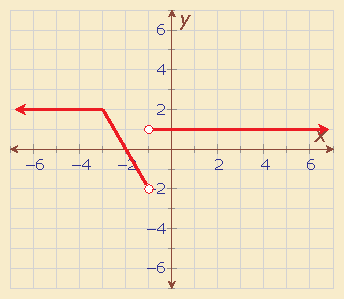
\includegraphics[scale=0.8]{../mathbook-caos-calculo/images/ejp-1-8-1g.pdf}}\hfill%
\subfigure[]{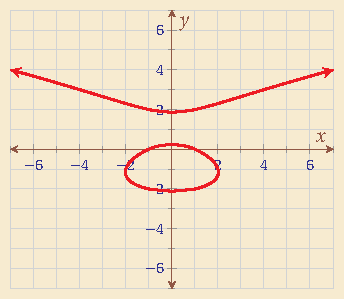
\includegraphics[scale=0.8]{../mathbook-caos-calculo/images/ejp-1-8-1h.pdf}}\hfill%
\subfigure[]{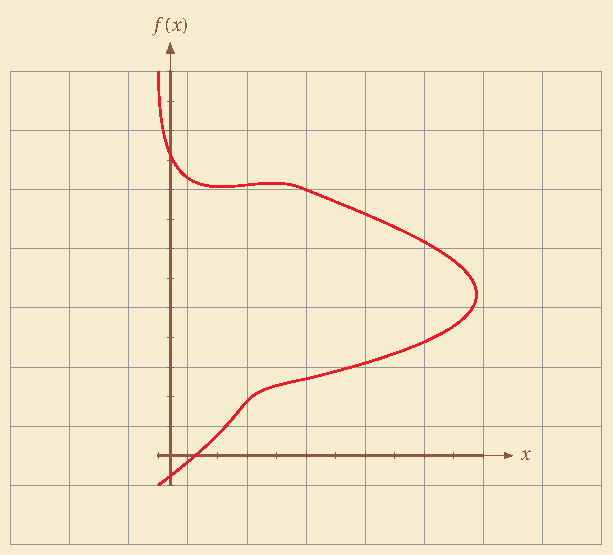
\includegraphics[scale=0.4]{../mathbook-caos-calculo/images/ejp-1-8-1c.pdf}}\\%
\subfigure[]{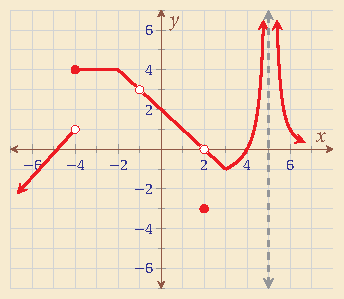
\includegraphics[scale=0.8]{../mathbook-caos-calculo/images/ejp-1-8-1e.pdf}}\hfill%
\subfigure[]{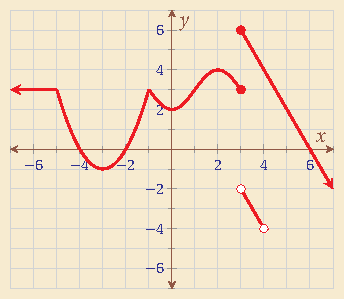
\includegraphics[scale=0.8]{../mathbook-caos-calculo/images/ejp-1-8-1f.pdf}}\hfill%
\subfigure[]{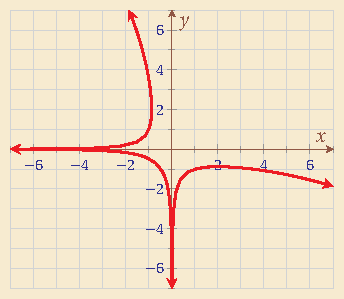
\includegraphics[scale=0.8]{../mathbook-caos-calculo/images/ejp-1-8-1j.pdf}}%
\end{figure}	
	

\item Un punto $P\left(  x,y\right)  $ se mueve, en sentido horario, sobre la
par\'{a}bola
\[
\left(  x-2\right)  ^{2}+16\left(  y+5\right)  =0.
\]
Exprese mediante una funci\'{o}n de variable real la distancia del punto
$P\left(  x,y\right)  $ al punto $A\left(  2,2\right)  .$

\item \label{cap1prob3}Una v\'{\i}a de ferrocarril cruza una carretera
formandose un \'{a}ngulo de $60^{0}$, como lo muestra la figura
\begin{center}
\includegraphics[scale=0.8]%
{../mathbook-caos-calculo/images/ejp-1-3.pdf}%
\end{center}

Una locomotora a $800$ metros de la intersecci\'{o}n se aleja de ella a
raz\'{o}n de $100\dfrac{km}{h}.$ Un automovil a $800$ metros de la
intersecci\'{o}n se acerca a ella a raz\'{o}n de $80\dfrac{km}{h}.$
\textquestiondown Cu\'{a}l es la distancia de separaci\'{o}n entre el
automovil y la locomotora en ese instante ?. Exprese mediante una funci\'{o}n
de variable real, dependiente del tiempo $t$, la distancia de separaci\'{o}n
entre la locomotora y el automovil$.$

\item Cierta cantidad de aceite fluye hacia el interior de un deposito en
forma de cono invertido a raz\'{o}n de $0.1\pi\,\frac{m^{3}}{\min}.$ El
deposito tiene un radio de $2.5m$ en su parte superior y una profundidad de
$10m$. Si el deposito inicialmente contiene $1.2m^{3}$ de aceite. Exprese
mediante una funci\'{o}n de variable real, dependiente de la altura $h$, la
cantidad de aceite del recipiente.%
\begin{center}
\includegraphics[scale=0.6]%
{../mathbook-caos-calculo/images/ejr-1-8-4.pdf}%
\end{center}




\item Sea $\triangle ABC$ is\'{o}sceles con $AB=AC,$ y $m\measuredangle
BAC=\alpha.$ Exprese mediante una funci\'{o}n de variable real, dependiente
del valor del \'{a}ngulo $\alpha,$ el \'{a}rea del $\triangle ABC$.

\item Una isla est\'{a} ubicada en el punto $A$, $4\,km$ mar adentro del punto
m\'{a}s cercano $B$ de una playa recta. Una atleta, en la isla desea ir al
punto $C$, a $6$ $km$ de $B$ playa abajo. La mujer debe dirigirse hacia un
punto $P$, entre $B$ y $C$, en un bote de remos a $3.5\dfrac{km}{h}$ y
desp\'{u}es caminar en forma recta de $P$ a $C$ a $6\dfrac{km}{h}.$ Exprese
mediante una funci\'{o}n de variable real, dependiente de $x=BP,$ el tiempo
necesario para viajar desde $A$ hacia $C,$ pasando por el punto $P$.
\begin{center}
\includegraphics[scale=0.3]%
{../mathbook-caos-calculo/images/ejp-1-6.pdf}%
\end{center}


\item Exprese mediante una funci\'{o}n de variable real, dependiente de $x,$
el \'{a}rea del rect\'{a}ngulo que tiene dos v\'{e}rtices en el eje $x$ y los
otros dos en la par\'{a}bola $y=16-x^{2},$ por arriba del eje $x.$

\item Hay que construir una pileta de las dimensiones que se muestran.
S\'{o}lo se puede variar el \'{a}ngulo $\theta$ . Exprese mediante una
funci\'{o}n de variable real, dependiente del \'{a}ngulo $\theta,$ el volumen
de la pileta.%
\begin{center}
\includegraphics[scale=0.3]%
{../mathbook-caos-calculo/images/ejr-1-8-8.pdf}%
\end{center}


\item Un granjero desea cercar tres terrenos rectangulares adyacentes
identicos, cada uno de ellos de 1800 pies cuadrados de \'{a}rea, incluyendo
cerca en medio de ellos. Exprese mediante una funci\'{o}n de variable real,
dependiente de la profundidad de los terrenos, el perimetro total para
realizar est\'{a} tarea.

\item Dada una esfera de radio $R$. Exprese mediante una funci\'{o}n de
variable real, dependiente de $R$, el volumen del cono circular recto de radio
$r$ y altura $h$ que puede inscribirse en la esfera.

\item Una particula se mueve a lo largo de una l\'{\i}nea recta, siendo su
posici\'{o}n $x\left(  t\right)  $ metros en todo tiempo $t>0$ segundos
\[
x\left(  t\right)  =\dfrac{5t+20}{t+1}+2t
\]


\begin{enumerate}
\item Completa la siguiente tabla:%
\[%
\begin{tabular}
[c]{|l|l|l|l|l|l|l|l|}\hline
$t\left[  s\right]  $ & $1$ & $2$ & $3$ & $4$ & $5$ & $6$ & $7$\\\hline
$x\left[  m\right]  $ &  &  &  &  &  &  & \\\hline
\end{tabular}
\ \
\]


\item Usa los resultados de la tabla para hacer un bosquejo de la gr\'{a}fica
de $x\left(  t\right)  .$ Con la ayuda de un software, gr\'{a}fique $x$ $vs$
$t.$ Compare y analice las gr\'{a}ficas.

\item \textquestiondown En qu\'{e} momento la part\'{\i}cula alcanza una
posici\'{o}n de $3$ metros?
\end{enumerate}

\item Una hoja de papel de dimensiones 12 cms por 8 cms , se corta por las
esquinas en cuadrados de $x$ cms de lado.

\begin{enumerate}
\item Muestre que el volumen que se puede construir a partir de la hoja viene
dado por $V(x)=4x(6-x)(4-x),0<x<4.$

\item Complete la siguiente tabla:%
\[%
\begin{tabular}
[c]{|l|l|l|l|l|l|}\hline
$x$ $\left[  cm\right]  $ & $0$ & $1$ & $2$ & $3$ & $4$\\\hline
$V$ $\left[  cm^{3}\right]  $ &  &  &  &  & \\\hline
\end{tabular}
\ .
\]


\item Estime el m\'{a}ximo volumen que puede tener la caja ( Explique sus procedimientos)
\end{enumerate}

\item Una funci\'{o}n est\'{a} definida por $f(x)=3x+1,$ $x\in R$. Determine
el conjunto soluci\'{o}n de la ecuaci\'{o}n $f(2x)-f(x+1)=4.$

\item Considere los conjuntos
\[
A=\{x\in\nz\mid x<5\},B=\{x\in\nz\mid3\leq x\leq5\}.
\]
Para cada una de las relaciones de $A$ a $B$ dadas a continuaci\'{o}n
determine su dominio y su rango. Haga una gr\'{a}fica de la relaci\'{o}n e
indique si la relaci\'{o}n dada es una funci\'{o}n. En caso de serlo indique
si es sobre, uno-a-uno o biyectiva. Justifique todas sus respuestas.

\begin{enumerate}
\item $R=\{(2,3),(3,5),(1,3),(4,4)\}$.

\item $S=\{(1,3),(2,3),(3,4),(4,5)\}$.

\item $T=\{(1,3),(1,4),(1,5)\}$.

\item $U=\{(1,3),(2,3),(3,3),(4,3)\}$.

\item $V=\{(1,4),(2,3)\}$.
\end{enumerate}

\item Considere, en cada caso, la funci\'{o}n de variable real $f$ definida
por la f\'{o}rmula dada. Determine dominio y rango de la funci\'{o}n e indique
si es sobre, uno-a-uno o biyectiva. Haga una gr\'{a}fica de la funci\'{o}n.
Indique tambi\'{e}n, si los hay, los valores m\'{a}ximo y m\'{\i}nimo de la funci\'{o}n.

\begin{enumerate}
\item $f(x)=x^{2}+3x+2$.

\item $f(x)=3x+7$.

\item $f(x)=3x^{2}+x-4$.

\item $f(x)=-x^{2}+x+1$.

\item $f(x)=\pi$.

\item $f(x)=2x^{2}-3x+5$.

\item $f(x)=|x-2|$.

\item $f(x)=|x^{2}+3x+2|$.
\end{enumerate}

\item Para cada una de las funciones del ejercicio anterior determine las
intersecciones de su gr\'{a}fica con los ejes coordenados. En cada caso
determine el dominio de la funci\'{o}n de variable real definida por la
f\'{o}rmula dada.

\begin{enumerate}
\item $f(x)=\sqrt{x^{2}+5x+6}$.

\item $f(x)=\dfrac{2-x}{x^{2}+5x+6}$.

\item $f(x)=\dfrac{\sqrt{2-x}}{x+3}$.

\item $f(x)=\dfrac{x+1}{3x^{2}+x+1}$.

\item $f(x)=\sqrt{|x|}$.

\item $f(x)=\sqrt{\dfrac{x-1}{2x+3}}$.

\item $f\left(  x\right)  =\sqrt{x^{2}+2x-15}$
\end{enumerate}

\item Considere la funci\'{o}n definida por $g(x)=x^{3}+x^{2}+1$.
\textquestiondown Est\'{a} $3$ en el rango de $g$? \textquestiondown Es $g$
una funci\'{o}n uno-a-uno?

\item Sea $f$ definida por $f(x)=\sqrt{2x+1}$. Encuentre los valores de $h$
para los cuales $2+h$ est\'{a} en:

\begin{enumerate}
\item El dominio de $f$.

\item El rango de $f$.
\end{enumerate}

\item En cada caso indique si la relaci\'{o}n real dada es una funci\'{o}n. En
caso afirmativo indique el dominio de la misma. En caso negativo, encuentre
una funci\'{o}n definida impl\'{\i}citamente por la ecuaci\'{o}n que define la relaci\'{o}n.

\begin{enumerate}
\item $R=\{(x,y)\mid x^{2}-y^{2}=1\}$.

\item $S=\{(x,y)\mid x^{2}+xy-3x=0\}$.

\item $T=\{(x,y)\mid x=1,x^{2}+x-y=0\}$.

\item $U=\{(t,u)\mid t^{2}+u^{2}-2u=0\}$.

\item $V=\{(t,s)\mid s^{3}+2s^{2}+s-t=0\}$.
\end{enumerate}

\item Considere la relaci\'{o}n $R=\{(x,y)\mid Ax^{2}+Cy^{2}+Dx+Ey+F=0\}$,
donde $A,C,D,E$ y $F$ son reales dados. Demuestre que:

\begin{enumerate}
\item Si $A=C\neq0$, la gr\'{a}fica de $R$ es una circunferencia, un punto o
el conjunto vac\'{\i}o.

\item Si $A=0$ o $C=0$, la gr\'{a}fica de $R$ es una par\'{a}bola, dos rectas
paralelas, una sola recta o el conjunto vac\'{\i}o.
\end{enumerate}

\item \label{ejercicio1} En cada caso determine el dominio de $f+g,fg$ y
$f/g$, para las funciones reales $f$ y $g$ definidas como se indica. Encuentre
adem\'{a}s
\[
(f+g)(x),(fg)(x),(f/g)(x)
\]
para $x$ en el dominio de la correspondiente funci\'{o}n.

\begin{enumerate}
\item $f(x)=\dfrac{x}{x-2},\ g(x)=\sqrt{x^{2}-x}$.

\item $f(x)=\dfrac{x-2}{x^{2}-3x+2},\ g(x)=\dfrac{2}{x+1}$.

\item $f(x)=\sqrt{x^{2}+3x+2},\ g(x)=\dfrac{x}{x+2}$.

\item $f(x)=\sqrt{x+1},\ g(x)=\sqrt{x^{2}+x+1}$.

\item $f(x)=\sqrt{\dfrac{x+1}{x-2}},\ g(x)=\sqrt{6+x-x^{2}}$.
\end{enumerate}

\item Como en el ejercicio anterior para las funciones
\[
f=\{(a,0),(b,1),(c,-3),(d,-5)\},\ g=\{(a,3),(b,-5),(c,6),(e,9)\}
\]


\item Sea $f$ la funci\'{o}n de variable real definida por $f(x)=5x+3$.
Determine todos los valores de $x$ para los cuales:

\begin{enumerate}
\item $f(2x)=2f(x)$.

\item $f(x+c)=f(x)+f(c)$, si $c$ es un real fijo dado.\newline Haga lo mismo
si $f(x)=5x$.
\end{enumerate}

\item Sea $f:\rz\longrightarrow\rz$ una funci\'{o}n. $f$ es una
\index{Aplicaci\'{o}n lineal|textbf}%
aplicaci\'{o}n lineal si, y solo si para todo $x_{1},x_{2}\in\rz$ se cumple
que $f(x_{1}+x_{2})=f(x_{1})+f(x_{2})$ y $f(x_{1}x_{2})=x_{1}f(x_{2})$.
Demuestre que el conjunto de todas las aplicaciones lineales de $\rz$ en
$\rz$, al cual notaremos $Lin(\rz,\rz)$, es cerrado para las operaciones de
adici\'{o}n de funciones y multiplicaci\'{o}n por funciones constantes. Es
decir, demuestre que si $f,g\in Lin(\rz,\rz)$ y $k\in\rz$ entonces:
\begin{align*}
(f+g)  &  \in Lin(\rz,\rz)\\
kf  &  \in Lin(\rz,\rz).
\end{align*}


\item Demuestre que una funci\'{o}n $f:\rz\longrightarrow\rz$ es una
aplicaci\'{o}n lineal si, y solo si existe una constante $k\in\rz$ tal que
$f(x)=kx$, para todo $x\in\rz$. As\'{\i}, toda aplicaci\'{o}n lineal es una
funci\'{o}n lineal. \textquestiondown Es verdadero el rec\'{\i}proco?.

\item En cada caso determine, si est\'{a}n definidas, las compuestas $f\circ
g$ y $g\circ f$, indicando sus dominios de definici\'{o}n.

\begin{enumerate}
\item $f=\{(a,1),(2,-3),(c,d),(0,5)\},\ g=\{(1,3),(5,6),(a,4)\}$.

\item $f=\{(3,2),(4,5),(6,7)\},\ g=\{(2,4),(5,6),(8,3)\}$.

\item $f$ y $g$ son funciones de variable real definidas por:

\begin{enumerate}
\item $f(x)=2,\ g(x)=5x$.

\item $f(x)=3,\ g(x)=2$.

\item $f(x)=x+1,\ g(x)=x-1$.

\item $f(x)=x^{2}+2x-3,\ g(x)=\sqrt{x}$.

\item $f(x)=\sqrt{x-2},\ g(x)=x^{3}$.

\item $f(x)=\dfrac{x}{x+3},g(x)=\sqrt{x+1}$.
\end{enumerate}
\end{enumerate}

\item En cada caso indique si la funci\'{o}n dada es invertible. En caso
afirmativo, encuentre su inversa. Si no es invertible, encuentre al menos dos
restricciones de la funci\'{o}n dada que sean invertibles y halle las inversas
de tales restricciones. Utilice software adecuado para graficar la funci\'{o}n
(o una restricci\'{o}n de la misma) y su inversa.

\begin{enumerate}
\item $f=\{(1,3),(\pi,5),(\sqrt{2},3),(5,7)\}$.

\item $g=\{(2,1),(3,5),(4,0),(6,1),(8,5)\}$.

\item La funci\'{o}n de variable real $f$ definida por:

\begin{enumerate}
\item $f(x)=5x-7$.

\item $f(x)=6$.

\item $f(x)=x$.

\item $f(x)=ax+b$, donde $a,b\in\rz$.

\item $f(x)=x^{2}-x-30$.

\item $f(x)=ax^{2}+bx+c$, donde $a,b$ y $c$ son reales cualesquiera con
$a\neq0$.

\item $f(x)=\sqrt{x}$.

\item $f(x)=x^{3}$.
\end{enumerate}
\end{enumerate}

\item Una funci\'{o}n $f:\rz\longrightarrow\rz$ se denomina localmente
invertible si existe un intervalo abierto $\left]  a,b\right[  $ tal que la
restricci\'{o}n $f|_{\left]  a,b\right[  }$ es invertible. En tal caso
$f|_{\left]  a,b\right[  }^{-1}$ es una inversa local de $f$. Encuentre al
menos dos inversas locales para la funci\'{o}n $f$ definida por:

\begin{enumerate}
\item $f(x)=x^{2}+3x+5$.

\item $f(x)=x^{3}$.
\end{enumerate}

\item Sea $f$ una funci\'{o}n real invertible \textquestiondown Se puede
afirmar que $f^{-1}=\dfrac{1}{f}$? Justifique su respuesta.

\item Sea $a$ un real positivo. Una funci\'{o}n $f:[-a,a]\longrightarrow\rz$
se denomina%
\index{Funci\'{o}n!-- par}
par si, y solo si
\[
f(-x)=f(x)\ \mbox{para todo \ }x\in\lbrack-a,a].
\]
$f$ es una funci\'{o}n impar%
\index{Funci\'{o}n!-- impar}
si, y solo si
\[
f(-x)=-f(x)\ \mbox{para todo \ }x\in\lbrack-a,a].
\]


\begin{enumerate}
\item Demuestre que si $f(x)=x^{2}+1$, entonces $f$ es par y que la
funci\'{o}n $g$ definida por $g(x)=x^{3}+x$ es impar.

\item \textquestiondown Es toda funci\'{o}n constante una funci\'{o}n par?

\item Demuestre que una funci\'{o}n lineal es par si, y solo si es constante e
impar si, y solo si es un m\'{u}ltiplo de la funci\'{o}n id\'{e}ntidad. En
particular, la funci\'{o}n identidad es impar.

\item Demuestre que la funci\'{o}n cuadr\'{a}tica $f(x)=ax^{2}+bx+c$ es una
funci\'{o}n par si, y solo si $b=0$. \textquestiondown Existen funciones
cuadr\'{a}ticas impares?.

\item Discuta la veracidad de la siguiente afirmaci\'{o}n:

Si $f$ es una funci\'{o}n par, su gr\'{a}fica es sim\'{e}trica respecto del
eje $Y$.
\end{enumerate}

\item En cada caso indique si la proposici\'{o}n dada es Verdadera o falsa.
Justifique sus respuestas.

\begin{enumerate}
\item Toda funci\'{o}n lineal es invertible.

\item Una funci\'{o}n lineal es invertible si, y solo si no es constante.

\item Toda funci\'{o}n lineal no constante es localmente invertible.

\item Toda funci\'{o}n cuadr\'{a}tica es invertible.

\item Ninguna funci\'{o}n cuadr\'{a}tica es invertible.

\item Toda funci\'{o}n cuadr\'{a}tica es localmente invertible.

\item Una funci\'{o}n real de variable real es invertible si, y solo si toda
recta paralela al eje $X$ que intersecte su gr\'{a}fica lo hace en un solo punto.

\item Una funci\'{o}n $f:\rz\longrightarrow\rz$ es par si, y solo toda recta
paralela al eje $X$ que intersecte la gr\'{a}fica de $f$ lo hace en al menos
dos puntos.
\end{enumerate}

\item Sea la funci\'{o}n $f(x)=2x^{2}+x-3$ y $g\left(  x\right)  =x^{3}-1$

\begin{enumerate}
\item Calcule $f+g,fg,\frac{f}{g}$ y sus respectivos dominios.

\item Calcule $\dfrac{f\left(  3+h\right)  -f\left(  3\right)  }{h}.$

\item Halle $\left(  f\circ f\right)  \left(  x\right)  ,\left(  f\circ
g\right)  \left(  x\right)  ,\left(  g\circ f\right)  \left(  x\right)
,\left(  g\circ g\right)  \left(  x\right)  $ y sus respectivos dominios.

\item Calcule $f\left(  f\left(  1\right)  \right)  ,\left(  f\circ g\right)
\left(  0\right)  ,\left(  g\circ f\right)  \left(  -1\right)  ,\left(  g\circ
g\right)  \left(  1\right)  .$
\end{enumerate}

\item Sean $f\left(  x\right)  =x^{4}+2x^{3}-3x^{2}-4x-5.$ y $g\left(
x\right)  =3x^{4}+2x^{3}+7x-5.$

\begin{enumerate}
\item Hallar $h_{1}\left(  x\right)  :=\dfrac{1}{2}\left[  f\left(  x\right)
+g\left(  x\right)  \right]  .$

\item Hallar $h_{2}\left(  x\right)  :=\dfrac{1}{2}\left[  f\left(  x\right)
-g\left(  x\right)  \right]  .$
\end{enumerate}

\item Consideremos la funci\'{o}n $f$ definida por $f(x)$ $=\dfrac{x^{2}%
-x+1}{x+2}$ para $x\geq0.$ \textquestiondown Existe alg\'{u}n valor$\ a$ del
dominio de la funci\'{o}n tal que $f(a)=a$?$.$

\item \label{cap1prob35}Sean las funciones: $f(x)=\dfrac{x^{2}-1}{x+1}$ y
$g(x)=$ $-\sqrt{x^{2}-\frac{1}{4}}.$ Hallar:\vspace{-0.9in}

\multicolsep2.5 cm \columnsep1 cm\begin{multicols}
{2}
\begin{enumerate}
\item$\operatorname*{Dom}(f)$
\item$\operatorname*{Dom}(g)$
\item$\left(  f + g\right)            \left(
x\right)            $ \item $\operatorname*{Dom}(f + g)$
\item$\left(            gf\right) \left(   x\right)
$ \item$\operatorname*{Dom}(gf)$ \item$g\left(  g\left(
x\right)            \right) $
\item$\left(  f\circ g\right)            \left(
x\right)
$ \item $\operatorname*{Dom}(f\circ g)$
\item$\left(            g\circ f\right) \left(   x\right)$
\item$\operatorname*{Dom}(g\circ f)$
\item $\operatorname*{Dom}(f/g)$
\end{enumerate}
\end{multicols}\vspace{-0.9in}

\item Realice el problema \ref{cap1prob35}, si:

\begin{enumerate}
\item $f\left(  x\right)  =\dfrac{1+2x}{x^{2}}$ y $g\left(  x\right)
=\sqrt{x-1}.$

\item $f\left(  x\right)  =\dfrac{x^{2}+9}{x^{4}-1}$ y $g\left(  x\right)
=\sqrt{8-x^{2}}.$

\item $f\left(  x\right)  =\dfrac{1}{x^{4}-13x^{2}+36}$ y $g\left(  x\right)
=\sqrt{x^{2}-1}.$
\end{enumerate}

\item Para cada una de las funciones $f,g,h$ dadas a continuaci\'{o}n halle el
dominio, el rango, y con ayuda de un software, elabore la gr\'{a}fica.

\begin{enumerate}
\item
\[
f\left(  x\right)  =\left\{
\begin{tabular}
[c]{cl}%
$\dfrac{x^{2}-9}{x-3}$ & , si $x\neq3$\\
\multicolumn{1}{l}{$1$} & , si $x=3.$%
\end{tabular}
\right.
\]


\item
\[
g\left(  x\right)  =\left\{
\begin{tabular}
[c]{ll}%
$\sqrt{x^{2}-4}$ & , si $x<1$\\
$2x-1$ & , si $x\geq1.$%
\end{tabular}
\ \ \right.
\]


\item
\[
h\left(  x\right)  =\dfrac{\left\vert x\right\vert }{x}%
\]

\end{enumerate}

\item Considerando las funciones del ejemplo anterior calcule $f+g,fg,h\circ
g,g\circ f$ y determine, para cada caso, el dominio respectivo.

\item Sea la funci\'{o}n%
\[
g\left(  x\right)  =\left\{
\begin{tabular}
[c]{ll}%
$x^{2}+3x-2$ & , si $0<x<1$\\
$x-1$ & , si $x\geq1.$%
\end{tabular}
\ \ \ \ \ \ \right.
\]
Calcule el dominio de $g$. \textquestiondown \ Las expresiones $g\left(
1\right)  ,g\left(  -1\right)  ,g\left(  0\right)  ,g\left(  \dfrac{1}%
{2}\right)  $ est\'{a}n bien definidas?. En caso afirmativo determine la
imagen, en caso negativo, Justifique.

\item Sea la funci\'{o}n $f\left(  x\right)  =\left\vert 3x-2\right\vert
+\left\vert x+1\right\vert $

\begin{enumerate}
\item Reescriba la funci\'{o}n sin barras de valor absoluto .

\item Elabore la gr\'{a}fica.

\item Calcule $f(\frac{2}{3}),f(\frac{3}{2}),f\left(  2\right)  ,f\left(
3\right)  .$
\end{enumerate}

\item Determine los dominios de cada una de las funciones dadas

\begin{enumerate}
\item
\[
h\left(  x\right)  =\sqrt{\allowbreak6x^{3}-5x^{2}-2x+1}.
\]


\item
\[
g\left(  u\right)  =\dfrac{5u+1}{\allowbreak6u^{3}+11u^{2}-3u-2}.
\]


\item
\[
f\left(  u\right)  =\dfrac{\sqrt{\allowbreak6u^{3}-5u^{2}-2u+1}}%
{\allowbreak6u^{3}+11u^{2}-3u-2}.
\]


\item
\[
s\left(  y\right)  =\dfrac{\sqrt{3y^{3}+y^{2}-6y-2}}{2y^{2}+y-3}.
\]


\item
\[
g\left(  t\right)  =\sqrt{\dfrac{5t-2}{t^{2}-1}}.
\]


\item
\[
g\left(  x\right)  =\sqrt{\dfrac{5x^{2}+2}{x^{2}-4}}.
\]


\item
\[
f\left(  x\right)  =\sqrt{\dfrac{x-2}{\left(  x^{2}+x-1\right)  \left(
1-2x^{2}\right)  }}.
\]


\item
\[
h\left(  z\right)  =\sqrt[3]{\dfrac{5z-2}{z^{2}-1}}.
\]


\item
\[
s\left(  x\right)  =\sqrt[7]{\dfrac{x^{5}+2x^{2}+2}{x^{2}+7x-1}}.
\]


\item
\[
t\left(  y\right)  =\dfrac{\sqrt{2y^{2}+y-1}}{\sqrt{7y-10y^{2}-1}}.
\]

\end{enumerate}

\item Si $F(x)=\sqrt{(x-3)(x-1)}$

\begin{enumerate}
\item Determine el dominio de $F$.

\item Pruebe que $F(2-\sqrt{10})=3$
\end{enumerate}

\item Si $g\left(  x\right)  =x^{2}+x-1$, calcule:

\begin{enumerate}
\item $\dfrac{g\left(  x+h\right)  -g\left(  x\right)  }{h}.$

\item $\dfrac{g\left(  x+\dfrac{1}{h}\right)  -g\left(  \dfrac{1}{h}\right)
}{x}.$

\item $g\left(  2x\right)  -g\left(  3x\right)  .$
\end{enumerate}

\item Pruebe que si $c\in\rz,\left\{  a_{i}\right\}  _{i\in\nz}$ y $\left\{
b_{i}\right\}  _{i\in\nz}$ sucesiones de n\'{u}meros reales, entonces

\begin{enumerate}
\item
\[
\sum_{i=1}^{n}{c=cn.}%
\]


\item
\[
\sum_{i=1}^{n}{ca_{i}=c}\sum_{i=1}^{n}{a_{i}.}%
\]


\item
\[
\sum_{i=1}^{n}\left(  {a_{i}+b_{i}}\right)  {=}\sum_{i=1}^{n}{a_{i}+}%
\sum_{i=1}^{n}{b_{i}.}%
\]

\end{enumerate}

\item Pruebe, utilizando inducci\'{o}n matem\'{a}tica, que el t\'{e}rmino
n-\'{e}simo de la serie asociada a la sucesi\'{o}n:

\begin{enumerate}
\item $\left\{  i\right\}  _{i\in\nz}$ est\'{a} dado por
\[
\frac{n(n+1)}{2}.
\]


\item $\left\{  i^{2}\right\}  _{i\in\nz}$ est\'{a} dado por
\[
\frac{n(n+1)(2n+1)}{6}.
\]


\item $\left\{  i^{3}\right\}  _{i\in\nz}$ est\'{a} dado por
\[
\frac{1}{4}n^{2}+\frac{1}{2}n^{3}+\frac{1}{4}n^{4}.
\]

\end{enumerate}

\item Calcule:

\begin{enumerate}
\item
\[
\sum_{k=4}^{22}{(k-8)^{2}.}%
\]


\item
\[
\sum_{n=1}^{5}\left(  n+3\right)  .
\]


\item
\[
\sum_{n=1}^{15}\left(  2n-1\right)  ^{2}.
\]


\item
\[
\sum_{n=1}^{350}n.
\]

\end{enumerate}

\item Encuentre una sucesi\'{o}n con dominio $\nz$ cuyo rango sea el mismo de
los conjuntos dados (los mismos t\'{e}rminos en el mismo orden). Adem\'{a}s
para cada una de las sucesiones, determine sus cinco primeros t\'{e}rminos.
Finalmente, determine los cinco primeros t\'{e}rminos de la serie asociada a
la sucesi\'{o}n.

\begin{enumerate}
\item $\{n^{2}\}_{n=0}^{\infty}$.

\item $\left\{  \frac{2n}{n-1}\right\}  _{n=2}^{\infty}$.

\item $\left\{  \frac{n}{n+1}\right\}  _{n=0}^{\infty}$.

\item $\left\{  \sqrt{n}\right\}  _{n=0}^{\infty}$.

\item $\left\{  \frac{n}{\sqrt{n-3}}\right\}  _{n=4}^{\infty}$.
\end{enumerate}

\item Un subconjunto $A$ de $\rz$ se denomina
\index{Conjunto!-- enumerable}%
contable o
\index{Conjunto!-- contable}%
enumerable si est\'{a} contenido en el rango de una sucesi\'{o}n. El conjunto
$A$ es finito, si es vac\'{\i}o o si existen un n\'{u}mero natural \ $k$ \ y
\ una funci\'{o}n biyectiva $f:\{x\in\nz\mid x\leq k\}\longrightarrow A$. Demuestre:

\begin{enumerate}
\item Todo conjunto finito de n\'{u}meros reales es contable.

\item $A$ es contable si, y solo si existen un subconjunto $J\subseteq\nz$ y
una funci\'{o}n biyectiva $\beta:J\longrightarrow A$.

\item los conjuntos $\nz,\gz$ y $\qz$ son contables.
\end{enumerate}

\item Cuales son los primeros $6$ terminos de cada una de las sucesiones que
poseen el t\'{e}rmino n-\'{e}simo dado.

\begin{enumerate}
\item $a_{n}=\dfrac{n-2}{n}.$

\item $a_{n}=\cos\left[  \left(  2n-1\right)  \dfrac{\pi}{2}\right]  .$

\item $a_{n}=\dfrac{\left(  -1\right)  ^{n-1}\sin\left(  \pi n\right)  }{n}$

\item $a_{n}=\sqrt[n]{n}.$

\item $a_{n}=\dfrac{3^{n}}{n!}.$

\item $a_{n}=\dfrac{\cos\left(  n\right)  }{n}.$

\item $a_{n}=%
%TCIMACRO{\dsum \limits_{k=1}^{n}}%
%BeginExpansion
{\displaystyle\sum\limits_{k=1}^{n}}
%EndExpansion
\dfrac{1}{k^{2}}.$

\item $a_{n}=%
%TCIMACRO{\dsum \limits_{k=1}^{n}}%
%BeginExpansion
{\displaystyle\sum\limits_{k=1}^{n}}
%EndExpansion
\dfrac{1}{k\left(  k+1\right)  }.$

\item $a_{n}=%
%TCIMACRO{\dsum \limits_{k=0}^{n}}%
%BeginExpansion
{\displaystyle\sum\limits_{k=0}^{n}}
%EndExpansion
\left(  \dfrac{2}{3}\right)  ^{k}.$
\end{enumerate}

\item Calcule la primeras 6 sumas parciales de las siguientes series.

\begin{enumerate}
\item $%
%TCIMACRO{\dsum \limits_{n=1}^{\infty}}%
%BeginExpansion
{\displaystyle\sum\limits_{n=1}^{\infty}}
%EndExpansion
\dfrac{1}{n^{2}}.$

\item $%
%TCIMACRO{\dsum \limits_{n=1}^{\infty}}%
%BeginExpansion
{\displaystyle\sum\limits_{n=1}^{\infty}}
%EndExpansion
\dfrac{1}{\left(  4n-3\right)  \left(  4n+1\right)  }.$

\item $%
%TCIMACRO{\dsum \limits_{n=1}^{\infty}}%
%BeginExpansion
{\displaystyle\sum\limits_{n=1}^{\infty}}
%EndExpansion
\dfrac{n}{n+1}.$

\item $%
%TCIMACRO{\dsum \limits_{n=1}^{\infty}}%
%BeginExpansion
{\displaystyle\sum\limits_{n=1}^{\infty}}
%EndExpansion
\left(  \dfrac{2}{5}\right)  ^{n}$

\item $%
%TCIMACRO{\dsum \limits_{n=1}^{\infty}}%
%BeginExpansion
{\displaystyle\sum\limits_{n=1}^{\infty}}
%EndExpansion
\dfrac{1}{3^{n}}.$

\item $%
%TCIMACRO{\dsum \limits_{n=1}^{\infty}}%
%BeginExpansion
{\displaystyle\sum\limits_{n=1}^{\infty}}
%EndExpansion
\left(  \dfrac{1}{n}-\dfrac{1}{n+1}\right)  .$

\item $%
%TCIMACRO{\dsum \limits_{n=0}^{\infty}}%
%BeginExpansion
{\displaystyle\sum\limits_{n=0}^{\infty}}
%EndExpansion
\dfrac{4^{n+1}}{5^{n}}.$

\item $%
%TCIMACRO{\dsum \limits_{n=1}^{\infty}}%
%BeginExpansion
{\displaystyle\sum\limits_{n=1}^{\infty}}
%EndExpansion
\dfrac{1}{e^{2n}}.$
\end{enumerate}
\end{enumerate}


%
\chapter{L\'{\i}mite y Continuidad}

En este cap\'{\i}tulo se presenta uno de los conceptos fundamentales del
C\'{a}lculo y, en general, del An\'{a}lisis matem\'{a}tico: El concepto de
l\'{\i}mite. En principio-y ese ser\'{a} el tratamiento del concepto en este
curso- la idea de l\'{\i}mite est\'{a} ligada a la de \textquotedblleft
distancia\textquotedblright\ o, m\'{a}s precisamente, a la de
\textquotedblleft cercan\'{\i}a \textquotedblright, por lo que nuestro
inter\'{e}s inicial estar\'{a} en definir formalmente lo que consideraremos
una \textquotedblleft distancia\textquotedblright\ tanto en el sentido
intuitivo, ligado a problemas de naturaleza f\'{\i}sica o geom\'{e}trica, como
en la abstracci\'{o}n del mismo.

\section{Topolog\'{\i}a de la recta real}

Para dos puntos cualesquiera $P$ y $Q$ de la recta real, la
\index{Distancia|textbf}%
distancia entre ellos viene dada por el real no negativo
\begin{equation}
d(P,Q)=|x_{1}-x_{2}|, \label{distanciaenR}%
\end{equation}
donde $x_{1}$ y $x_{2}$ son las coordenadas de los puntos $P$ y $Q$,
respectivamente. Diremos tambi\'{e}n que tal distancia es la distancia entre
los reales $x_{1}$ y $x_{2}$. La distancia definida en $\rz$ por la
ecuaci\'{o}n (\ref{distanciaenR}) tiene algunas propiedades b\'{a}sicas
importantes, las cuales se desprenden de las propiedades del valor absoluto de
reales. Algunas de \'{e}stas \'{u}ltimas se enuncian a continuaci\'{o}n.
Suponemos $x,y\in\rz$:
\begin{align}
|x|  &  \geq0\\
|x|=0  &  \Longleftrightarrow x=0\\
|x+y|  &  \leq|x|+|y|\label{triangular1}\\
|xy|  &  =|x||y|
\end{align}
De las anteriores se siguen las siguientes propiedades de la distancia en
$\rz$.%
\index{Distancia!Propiedades de la --}%


\begin{theorem}
Sean $x,y,z$ n\'{u}meros reales, entonces:
\begin{align}
|x-y|  &  \geq0\label{nonegativa}\\
|x-y|=0  &  \Longleftrightarrow x=y\label{nulidad}\\
|x-y|  &  =|y-x|\label{simetria}\\
|x-y|  &  \leq|x-z|+|y-z| \label{triangular}%
\end{align}

\end{theorem}

La desigualdad (\ref{triangular1}) (y tambi\'{e}n su consecuencia
(\ref{triangular})) se acostumbra a denominar desigualdad triangular.

Definimos a continuaci\'{o}n conceptos importantes en la forma\-lizaci\'{o}n
del concepto de l\'{\i}mite, entre ellos el de vecindad.

\begin{definition}
Sean $c,r\in\rz$, con $r>0$. El intervalo abierto \textbf{centrado} en $c$ y
con radio $r$ es el intervalo
\[
]c-r,c+r[.
\]
Todo subconjunto de $\rz$ que contenga un intervalo abierto centrado en $c$ se
denomina una
\index{Vecindad|textbf}%
\textbf{vecindad} de $c$. En particular, todo intervalo abierto centrado en
$c$ es una vecindad de $c$.
\end{definition}
%TODO ---------
Se sigue f\'{a}cilmente que el intervalo con centro en $c$ y radio $r$ es el
conjunto de reales cuya distancia al centro es menor que el radio. En efecto,
tenemos:
\begin{align*}
x\in]c-r,c+r[  &  \Longleftrightarrow c-r<x<c+r\\
&  \Longleftrightarrow-r<x-c<r\\
&  \Longleftrightarrow|x-c|<r
\end{align*}
El intervalo $]a,b[=\{x\in\rz\mid a<x<b\}$ es claramente un intervalo abierto
centrado en $c=\frac{a+b}{2}$ y con radio $r=\frac{b-a}{2}$:
\begin{align*}
c-r  &  =\frac{a+b}{2}-\frac{b-a}{2}\\
&  =a\\
c+r  &  =\frac{a+b}{2}+\frac{b-a}{2}\\
&  =b
\end{align*}
%

\begin{figure}[H]
\centering
\includegraphics[scale=0.8]%
{fig2-1.pdf}%
\caption{Vecindades de $c$}%
\label{tiende2}%
\end{figure}



Podemos ahora formalizar, en t\'{e}rmino de vecindades, la noci\'{o}n de
proxi\-midad entre puntos de la recta real o, si se prefiere, entre
n\'{u}meros reales. Si $c$ es un real fijo, un real $x$ es \textquotedblleft%
\textit{cercano}\textquotedblright\ a $c$ si est\'{a} contenido en una
vecindad \textquotedblleft\textit{peque\~{n}a}\textquotedblright\ de $c$,
m\'{a}s precisamente, si pertenece a un intervalo centrado en $c$ y de radio
peque\~{n}o. As\'{\i}, la expresi\'{o}n \textquotedblleft\emph{la variable
real }$x$\emph{ tiende a }$c$\textquotedblright\ se interpreta diciendo que
$x$ toma valores en intervalos centrados en $c$ con radios cada vez menores
(ver figura \ref{tiende2}).

Terminamos esta secci\'{o}n con el concepto de punto de acumulaci\'{o}n de un
conjunto de n\'{u}meros reales. Intuitivamente hablando, un real $c$ es punto
de acumulaci\'{o}n de un conjunto $A$, si en las vecindades de $c$ se acumulan
en \textquotedblleft gran cantidad\textquotedblright\ elementos de tal conjunto.

\begin{definition}
Sean $A\subseteq\rz$ y $c\in\rz$. $c$ es un%
\index{Punto de acumulaci\'{o}n|textbf}
\underline{punto de} \underline{acumulaci\'{o}n} de $A$ si, y s\'{o}lo si toda
vecindad de $c$ contiene elementos de $A$ distintos de $c$.
\end{definition}

De la definici\'{o}n anterior, se sigue que si $c$ es punto de acumulaci\'{o}n
de $A$ toda vecindad de $c$ contiene infinitos elementos de $A$. En
consecuencia, ning\'{u}n conjunto finito tiene puntos de acumulaci\'{o}n.

\section{L\'{\i}mite de sucesiones}

Consideremos, como ejemplo introductorio, la sucesi\'{o}n $\left\{  \frac
{1}{n}\right\}  _{n\in\nz}$. Intuitivamente es claro que a medida que $n$ toma
valores m\'{a}s grandes, los valores de la sucesi\'{o}n son cada vez m\'{a}s
cercanos a cero. La tabla siguiente lo ilustra.

\begin{center}%
\begin{tabular}
[c]{|l||l|l|l|l|l|l|l|}\hline
$n$ & $1$ & $2$ & $3$ & $\dots$ & $50$ & $10^{6}$ & $10^{10}$\\\hline
$\frac{1}{n}$ & $1$ & $0.5$ & $0.333...$ & $\dots$ & $0.02$ & $0.000001$ &
$0.0000000001$\\\hline
\end{tabular}



\end{center}

El que, como lo sugiere la tabla anterior, $\frac{1}{n}$ tienda a cero
significa que toda vecindad de cero contiene a la \textquotedblleft
mayor\'{\i}a\textquotedblright\ de los t\'{e}rminos de la sucesi\'{o}n.
N\'{o}tese, en efecto, que si conside\-ramos intervalos centrados en cero y
con radios arbitrariamente peque\~{n}os, en cada caso solo un n\'{u}mero
finito de t\'{e}rminos de la sucesi\'{o}n se quedan por fuera del intervalo.
As\'{\i}, por ejemplo, para un radio $r=\frac{1}{5}$, todos los t\'{e}rminos
$\frac{1}{n}$ para $n\geq6$, est\'{a}n en el intervalo con centro en $0$ y
dicho radio $\frac{1}{5}$ (ver figura \ref{vecinocero2}).%


%TODO
\begin{figure}[H]
\centering
\includegraphics[scale=0.8]%
{fig-2-2.pdf}%
\caption{Vecindades de $c$}%
\label{vecinocero2}%
\end{figure}
%TODO 
En general, si $r>0$, existe un n\'{u}mero natural $N$ tal que $N>\frac{1}{r}%
$, por lo que para todo $n\geq N$ se tiene que
\begin{align*}
n>\frac{1}{r}  &  \Longrightarrow\frac{1}{n}<r\\
&  \Longrightarrow\left\vert \frac{1}{n}-0\right\vert <r
\end{align*}
lo que muestra que todos los t\'{e}rminos de la sucesi\'{o}n, a partir del
valor $n=N$, est\'{a}n en el intervalo centrado en $0$ y con radio $r$. Este
hecho se expresa diciendo que
\[
\lim_{n\rightarrow\infty}\frac{1}{n}=0
\]


La definici\'{o}n formal de l\'{\i}mite de una sucesi\'{o}n es como sigue. Sin
p\'{e}rdida de generalidad, como se explic\'{o} en el cap\'{\i}tulo anterior,
supondremos que el dominio de la sucesi\'{o}n es $\nz$.

\begin{definition}
\label{limitesucesion}%
\index{Sucesi\'{o}n!-- convergente}
Sea $\{x_{n}\}_{n\in\nz}$ una sucesi\'{o}n real. Decimos que la sucesi\'{o}n
es \textbf{convergente} si, y s\'{o}lo si existe un real $L$, tal que para
todo $r>0$, existe un n\'{u}mero natural $N$ tal que
\begin{equation}
|x_{n}-L|<r,\mbox{ \ siempre que \ }n\geq N \label{deflimitesucesion}%
\end{equation}
El real $L$ es el l\'{\i}mite de la sucesi\'{o}n%
\index{Sucesi\'{o}n!L\'{\i}mite de una --}
$\{x_{n}\}_{n\in\nz}$. Tal l\'{\i}mite es \'{u}nico (ver ejercicios) y decimos
que $x_{n}$ converge a $L$ y escribiremos
\[
\lim_{n\rightarrow\infty}x_{n}=L.
\]
Tambi\'{e}n es costumbre abreviar la expresi\'{o}n anterior escribiendo
$x_{n}\rightarrow L$.
\end{definition}

Como se anticip\'{o}, la ecuaci\'{o}n \ref{deflimitesucesion} establece que
todo intervalo abierto centrado en (toda vecindad de ) $L$ contiene a todos
los t\'{e}rminos de la sucesi\'{o}n, excepto a un n\'{u}mero finito de ellos.
Una sucesi\'{o}n no convergente se denomina divergente%
\index{Sucesi\'{o}n!-- divergente}%
.

La definici\'{o}n \ref{limitesucesion} no suministra herramientas
pr\'{a}cticas para el c\'{a}lculo de l\'{\i}mites. De hecho, la existencia
misma del l\'{\i}mite, como veremos, podr\'{\i}a establecerse sin conocerlo
espec\'{\i}ficamente. En la pr\'{a}ctica, necesitamos algunas herramientas que
nos permitan determinar tanto la existencia del l\'{\i}mite, como el
l\'{\i}mite mismo. Los teoremas que siguen apuntan en esa direcci\'{o}n,
aunque debe advertirse que, en general, no existen f\'{o}rmulas o
\textquotedblleft reglas m\'{a}gicas\textquotedblright\ que nos permitan
determinar l\'{\i}mites de sucesiones reales en cualquier caso.

Una de las propiedades b\'{a}sicas de una sucesi\'{o}n convergente es el que
su rango es un conjunto acotado%
\index{Conjunto!-- acotado}%
, lo cual significa que est\'{a} contenido en un intervalo de longitud finita.

\begin{theorem}
Sea $\{x_{n}\}_{n\in\nz}$ una sucesi\'{o}n convergente, entonces existe una
constante positiva $K$ tal que para todo $n\in\nz$ se tiene
\begin{equation}
|x_{n}|\leq K \label{acotada}%
\end{equation}

\end{theorem}

\begin{proof}
Sea $L$ el l\'{\i}mite de la sucesi\'{o}n $\{x_{n}\}_{n\in\nz}$. Entonces,
para $r=1$, se tiene que existe un n\'{u}mero natural $N$ tal que
\[
|x_{n}-L|<1,
\]
para $n\geq N$. Se tiene entonces que para $n\geq N$:
\begin{align*}
|x_{n}|  &  =|x_{n}-L+L|\\
&  \leq|x_{n}-L|+|L|\\
&  \leq1+L
\end{align*}
Escogiendo $K=Max\{1+L,|x_{n}|\mid n<N\}$ se tiene que $|x_{n}|\leq K$, para
todo natural $n$.
\end{proof}

El siguiente resultado puede ser de gran utilidad. B\'{a}sicamente, transforma
el problema de la convergencia de una sucesi\'{o}n a un real $L$ en el de la
convergencia a cero. Es una consecuencia inmediata de la definici\'{o}n.

\begin{theorem}
Sean $\{x_{n}\}_{n\in\nz}$ una sucesi\'{o}n y $L$ un n\'{u}mero real.
Entonces:
\begin{equation}
\lim_{n\rightarrow\infty}x_{n}=L\Longleftrightarrow\lim_{n\rightarrow\infty
}|x_{n}-L|=0
\end{equation}

\end{theorem}

El teorema anterior establece un hecho intuitivamente claro: Los valores de la
sucesi\'{o}n se aproximan a $L$ si, y solo si la distancia entre los
t\'{e}rminos de la sucesi\'{o}n y $L$ es pr\'{o}xima a cero. El teorema
siguiente ser\'{a} de gran utilidad en el c\'{a}lculo de l\'{\i}mites de
sucesiones cuando se conocen los l\'{\i}mites de otras sucesiones dadas.

\begin{theorem}%
\index{Sucesiones!Algebra de --}%
\label{algebrasucesiones} Sean $\{x_{n}\}_{n\in\nz},\{y_{n}\}_{n\in\nz}$
sucesiones reales convergentes a $L_{1}$ y $L_{2}$, respectivamente.
Entonces:
\begin{align}
x_{n}+y_{n}  &  \rightarrow L_{1}+L_{2}\label{sumasucesion}\\
x_{n}-y_{n}  &  \rightarrow L_{1}-L_{2}\\
x_{n}y_{n}  &  \rightarrow L_{1}L_{2}\label{productosucesion}\\
cx_{n}  &  \rightarrow cL_{1},c\in\rz
\end{align}

\end{theorem}

Tambi\'{e}n es claro que si una sucesi\'{o}n $\{x_{n}\}$ converge a cero su
producto por una sucesi\'{o}n convergente $\{y_{n}\}$ es tambi\'{e}n
convergente a cero. Sin embargo, una condici\'{o}n m\'{a}s d\'{e}bil que la
convergencia para $\{y_{n}\}$, como el ser acotada, garantiza tambi\'{e}n la
convergencia a cero del producto. Antes demostramos un importante criterio de comparaci\'{o}n.

\begin{theorem}
\label{emparedado}%
\index{Teorema!-- del emparedado}
Sean $\{x_{n}\}_{n\in\nz},\{y_{n}\}_{n\in\nz}$ sucesiones reales. Si existe un
$n_{0}\in\nz$ tal que
\[
|y_{n}|\leq|x_{n}|,\mbox{ \ para todo \ }n\geq n_{0},
\]
entonces $y_{n}\rightarrow0$ si $x_{n}\rightarrow0$.
\end{theorem}

\begin{proof}
Supongamos que $x_{n}$ converge a cero. Entonces para $r>0$ se tiene que
existe $N\in\nz$ tal que $|x_{n}|<r$, siempre que $n\geq N$. Si escogemos
$N_{1}=Max\{N,n_{0}\}$ entonces para $n\geq N_{1}$ tenemos
\[
|y_{n}|\leq|x_{n}|<r
\]
y as\'{\i} $y_{n}\rightarrow0$.
\end{proof}

El teorema anterior es usualmente conocido como un criterio tipo
\textquotedblleft\textit{emparedado}\textquotedblright. La sucesi\'{o}n
$x_{n}$ es una sucesi\'{o}n \textquotedblleft mayorante\textquotedblright\ de
$y_{n}$ que al ser convergente a cero, \textquotedblleft
obliga\textquotedblright\ a $y_{n}$ a converger tambi\'{e}n a cero.

Si $\{y_{n}\}_{n=n_{0}}^{\infty}$ es una sucesi\'{o}n real, hemos visto que
existe una sucesi\'{o}n $\{z_{n}\}_{n\in\nz}$ tal que los t\'{e}rminos de
ambas son iguales, por lo que podr\'{\i}an considerarse iguales. Es claro que
ambas sucesiones son o convergentes al mismo real o divergentes ambas. En tal
sentido, si $\{y_{n}\}_{n\in\nz}$ es una sucesi\'{o}n real tal que para
alg\'{u}n $n_{0}$ se tiene que $y_{n}\neq0$ si $n\geq n_{0}$, entonces podemos
definir la sucesi\'{o}n cociente
\[
\left\{  \frac{x_{n}}{y_{n}}\right\}  _{n=n_{0}}^{\infty}%
\]
la cual produce los mismos valores que la sucesi\'{o}n $\left\{  \frac{x_{n}%
}{z_{n}}\right\}  _{n\in\nz}.$ Supongamos, en particular, que se tiene el
cociente $\frac{1}{y_{n}}$, con $\{y_{n}\}_{n=n_{0}}^{\infty}$ y $y_{n}\neq0$.
Si $y_{n}\rightarrow L$ con $L\neq0$, entonces existe $N\in\nz$ tal que para
todo $n\geq N$ se cumple
\[
|y_{n}-L|<|L/2|.
\]
En consecuencia tenemos $-|L/2|\leq y_{n}-L\leq|L/2|,$ de donde se obtiene que
$|y_{n}|>|L/2|$ y, por lo tanto,
\[
\left\vert \frac{1}{y_{n}}\right\vert \leq\left\vert \frac{2}{L}\right\vert
=K;
\]
lo que significa que $\left\{  \frac{1}{y_{n}}\right\}  _{n=n_{0}}^{\infty}$
es una sucesi\'{o}n acotada. Como consecuencia:
\begin{align*}
\left\vert \frac{1}{y_{n}}-\frac{1}{L}\right\vert  &  =\left\vert \frac
{1}{y_{n}}\left(  \frac{L-y_{n}}{L}\right)  \right\vert \\
&  \leq\frac{K}{L_{1}}|y_{n}-L|\rightarrow0
\end{align*}
Tenemos entonces:

\begin{theorem}
Si $y_{n}\rightarrow L\neq0$, entonces $\dfrac{1}{y_{n}}\rightarrow\dfrac
{1}{L}$
\end{theorem}

Como un corolario tenemos entonces:

\begin{corollary}
Si $x_{n}\to L_{1}, y_{n}\to L_{2}$ y si $L_{2}\neq0$, entonces
\[
\frac{x_{n}}{y_{n}}\to\frac{L_{1}}{L_{2}}.
\]

\end{corollary}

Una sucesi\'{o}n real $\{x_{n}\}_{n\in\nz}$ diverge a $+\infty$, si para todo
real $L>0$, existe un $N\in\nz$ tal que $x_{n}>L$ para todo $n\geq N$. Esto
significa que la sucesi\'{o}n puede tomar va\-lores arbitrariamente grandes.
En tal caso escribimos
\[
\lim_{n\rightarrow\infty}x_{n}=+\infty.
\]


El siguiente teorema permite conocer algunos l\'{\i}mites notables.

\begin{theorem}
\label{enealap} Sea $p$ un n\'{u}mero real. Consideremos la sucesi\'{o}n
$\{x_{n}\}_{n\in\nz}$, definida por $x_{n}=n^{p}$. Entonces:

\begin{enumerate}
\item Si $p>0$, entonces $x_{n}$ es divergente a $+\infty$.

\item Si $p=0$, entonces $x_{n}\rightarrow1$.

\item Si $p<0$, entonces $x_{n}\rightarrow0$.
\end{enumerate}
\end{theorem}

\begin{proof}
\begin{enumerate}
\item Sea $p>0$, entonces para todo real positivo $L$ existe un n\'{u}mero
natural $N$ tal que $N\geq L^{1/p}$ ( si no fuera as\'{\i} $\nz$ ser\'{\i}a un
conjunto acotado superiormente). Se sigue que $N^{p}\geq L$ para alg\'{u}n
natural $N$ y, por tanto, para $n\geq N$, se tiene $n^{p}\geq L$, por lo que
la sucesi\'{o}n $\{n^{p}\}_{n\in\nz}$ diverge a $+\infty$.

\item Para $p=0$ el resultado es claro, pues se tiene la sucesi\'{o}n
constante $1$.

\item Consideremos finalmente el caso $p<0$. Como $-p>0$, la sucesi\'{o}n
$\{n^{-p}\}_{n\in\nz}$ es divergente a $+\infty$. Por lo tanto si $r>0$,
existe un n\'{u}mero natural $N$ tal que $N^{-p}>\frac{1}{r}$. Si $n\in\nz$ es
tal que $n\geq N$, entonces se tiene que
\[
n^{-p}\geq N^{-p}>\frac{1}{r}.
\]
As\'{\i}, para todo $n\geq N$:
\[
|n^{p}|=(n^{-p})^{-1}<r
\]
En consecuencia $n^{p}\rightarrow0$ si $p<0$.
\end{enumerate}
\end{proof}

En la demostraci\'{o}n del teorema siguiente se usa el Teorema del binomio%
\index{Teorema!-- del binomio}%
: Si $a,b\in\rz$ y $n\in\nz$, entonces:
\begin{equation}
(a+b)^{n}=\sum_{k=0}^{n}\dbinom{n}{k}a^{k}b^{n-k},
\end{equation}
donde $\dbinom{n}{k}=\dfrac{n!}{k!(n-k)!}$ es el coeficiente binomial. En
particular, si $a,b\geq0$, entonces para cada $k=0,\dots,n$ y $m\leq n$ se
tienen
\begin{align}
(a+b)^{n}  &  \geq\dbinom{n}{k}a^{k}b^{n-k}\\
(a+b)^{n}  &  \geq\sum_{k^{=}0}^{m}\dbinom{n}{k}a^{k}b^{n-k}%
\end{align}


\begin{theorem}
\label{raizndep} \hfil
\begin{enumerate}
\item Si $p>0$, entonces $\sqrt[n]{p}\rightarrow1$.

\item $\sqrt[n]{n}\rightarrow1$.

\item Sea $p>0$, entonces
\[
p^{n}\rightarrow\left\{
\begin{tabular}
[c]{ll}%
$+\infty$ & , si $p>1$\\
$0$ & , si $p<1$\\
$1$ & , si $p=1$%
\end{tabular}
\right.
\]


\item Si $x_{n}\geq0$ y $x_{n}\rightarrow L$, entonces $L\geq0$ y
$\sqrt[k]{x_{n}}\rightarrow\sqrt[k]{L}$.
\end{enumerate}
\end{theorem}

\begin{proof}
\footnote{La mayor parte de la demostraci\'{o}n de este teorema es tomada de
\cite{Rudin}} \hfill

\begin{enumerate}
\item Sea $x_{n}=\sqrt[n]{p}-1$. Si $p>1$, entonces $x_{n}>0$ y
\[
p=(1+x_{n})^{n}\geq1+nx_{n},
\]
de donde se sigue que $0\leq|x_{n}|\leq\frac{p-1}{n}$ y, por lo tanto,
$|x_{n}|\rightarrow0$, o sea $\sqrt[n]{p}\rightarrow1$. Si $p=1$, entonces
$x_{n}$ es la sucesi\'{o}n constante nula y el resultado se sigue. Para
$0<p<1$, se tiene $p^{-1}>1$, por lo que
\[
\lim_{n\rightarrow\infty}\sqrt[n]{p}=\lim_{n\rightarrow\infty}\frac
{1}{\sqrt[n]{p^{-1}}}=\frac{1}{1}=1.
\]


\item Como en la prueba anterior, sea $x_{n}=\sqrt[n]{n}-1\geq0$, entonces
\[
n=(1+x_{n})^{n}\geq\frac{n(n-1)}{2}x_{n}^{2},
\]
de donde
\[
0\leq x_{n}\leq\frac{\sqrt{2}}{\sqrt{n-1}}.
\]
Como
\[
\left\{  \frac{1}{n-1}\right\}  _{n=2}^{\infty}=\left\{  \frac{1}{n}\right\}
_{n\in\nz}%
\]
entonces $\sqrt{2}/\sqrt{n-1}\rightarrow0$ y, en consecuencia, $x_{n}%
\rightarrow0$.

\item Si $p>1$, entonces $p-1>0$. Supongamos ahora $L>0$, entonces
$\lim\limits_{n\rightarrow\infty}\sqrt[n]{L}=1$ y existe un n\'{u}mero natural
$N$ tal que
\[
|\sqrt[n]{L}-1|<p-1,
\]
siempre que $n\geq N$, de donde se sigue que para todo $n\geq N$
\[
0<\sqrt[n]{L}<p\ ;
\]
es decir, $L<p^{n}$. As\'{\i}, $p^{n}\rightarrow+\infty$. Para $p=1$, el
resultado es trivial. Si $0<p<1$, entonces $p^{-1}>1$ y $(p^{-1})^{n}$ diverge
a $+\infty$, por lo que dado un real positivo $r$, existe $n\in\nz$ tal que
\[
0<\frac{1}{r}<p^{-n},
\]
para todo $n\in\nz$. As\'{\i}, para $n\geq N$ se tiene $0<p^{n}<r$. Por lo
tanto $p^{n}\rightarrow0$.

\item Se deja de ejercicio.
\end{enumerate}
\end{proof}

\section{La serie geom\'{e}trica}%

\index{Serie!-- geom\'{e}trica}%
La sucesi\'{o}n $\{x^{n}\}_{n\in\nz_{0}}$ para $x\in\rz$, genera la serie
\[
\sum_{n=0}^{\infty}x^{n}.
\]
Recordemos que tal serie es la sucesi\'{o}n de sumas parciales
\[
1,1+x,1+x+x^{2},\dots,\sum_{k=0}^{n}x^{k},\dots
\]
Del teorema \ref{raizndep} se sigue que
\begin{equation}
x^{n}\rightarrow0\mbox{ \ si \ }|x|<1 \label{geometricaconvergente}%
\end{equation}
Es claro, adem\'{a}s, que $1^{n}\rightarrow1$ y que $(-1)^{n}$ es divergente.
Para $|x|>1$, la sucesi\'{o}n $\{x^{n}\}_{n\in\nz_{0}}$ no es acotada, pues la
sucesi\'{o}n $|x^{n}|$ diverge a $+\infty$. Por lo que $\{x_{n}\}_{n\in
\nz_{0}}$ es divergente \textquestiondown C\'{o}mo son las series asociadas?

Consideremos, para $x\neq1$ la identidad
\[
1-x^{n+1}=(1-x)(1+x+x^{2}+\dots+x^{n})=(1-x)\sum_{k=0}^{n}x^{k}.
\]
Despejando la $n-$\'{e}sima suma parcial de la sucesi\'{o}n$\{x^{n}%
\}_{n\in\nz}$ tenemos:
\begin{align*}
\sum_{k=0}^{n}x^{k}  &  =1+x+x^{2}+\dots+x^{n}\\
&  =\frac{1-x^{n+1}}{1-x}\\
&  =\frac{1}{1-x}-\frac{x}{1-x}x^{n}%
\end{align*}
Es claro que la serie converge si, y solo si lo hace la sucesi\'{o}n $\frac
{x}{1-x}x^{n}$. Esta \'{u}ltima, a su vez, converge si lo hace $x^{n}$, pues
$\frac{x}{1-x}$ es constante. Por lo tanto, tenemos

\begin{corollary}
\label{seriegeometrica} $\sum_{k=0}^{n} x^{k}$ converge si, y solo si $\vert x
\vert<1$. En tal caso
\begin{equation}
\label{convergeometrica}\sum_{n=0}^{\infty}x^{n}=\lim_{n\to\infty}
(1+x+\dots+x^{n})=\frac{1}{1-x}%
\end{equation}

\end{corollary}

As\'{\i}, por ejemplo,
\begin{align*}
\lim_{n\rightarrow\infty}\sum_{k=0}^{n}\left(  \frac{1}{2}\right)  ^{k}  &
=1+\frac{1}{2}+\frac{1}{4}+\frac{1}{8}+\dots\\
&  =\frac{1}{1-\frac{1}{2}}\\
&  =2\\
\sum_{n=0}^{\infty}\left(  -\frac{1}{3}\right)  ^{n}  &  =\frac{1}{1+(1/3)}\\
&  =\frac{3}{4}%
\end{align*}


\section*{El n\'{u}mero de Euler}

Una sucesi\'{o}n $\{x_{n}\}_{n\in\nz}$ de n\'{u}meros reales se denomina
creciente%
\index{Sucesi\'{o}n!-- creciente}
si $x_{n}\geq x_{m}$, siempre que $x_{n}\geq x_{m}$. Si $\{-x_{n}\}_{n\in\nz}$
es creciente, decimos que $\{x_{n}\}_{n\in\nz}$ es decreciente%
\index{Sucesi\'{o}n!-- decreciente}%
. Una sucesi\'{o}n
\index{Sucesi\'{o}n!-- mon\'{o}tona}%
es mon\'{o}tona si es o creciente o decreciente. Sucesiones mon\'{o}tonas son
convergentes si, y solo si son acotadas, como lo establece el siguiente
teorema. Lo demostramos solo para sucesiones crecientes.

\begin{theorem}
Una sucesi\'{o}n mon\'{o}tona%
\index{Sucesi\'{o}n!-- mon\'{o}tona!convergente|textit}
de n\'{u}meros reales converge si, y solo si es acotada.
\end{theorem}

\begin{proof}
Sea $\{x_{n}\}_{n\in\nz}$ creciente y acotada. Entonces, existe una cota
superior m\'{\i}nima, $L$, del rango de la sucesi\'{o}n. Es decir, $x_{n}\leq
L$ para todo $n\in\nz_{0}$ y para todo $K$ tal que $x_{n}\leq K$ para todo
$n$, se tiene que $L\leq K$.\newline Supongamos ahora que $r>0$, entonces
$L-r<L$ y, por lo tanto, no puede ser una cota superior para el rango de la
sucesi\'{o}n. As\'{\i}, existe $N\in\nz$, tal que
\[
L-r<x_{N}\leq L<L+r,
\]
de donde se sigue que para todo $n\geq N$
\[
L-r<x_{n}<L+r\ ;
\]
es decir, $|x_{n}-L|<r$, para todo $n\geq N$. Por lo tanto
\[
\lim_{n\rightarrow\infty}x_{n}=L.
\]

\end{proof}

Como una aplicaci\'{o}n importante del teorema anterior, consideremos la
sucesi\'{o}n
\[
\left\{  \frac{1}{n!}\right\}  _{n\in\nz_{0}}=\left\{  1,1,\frac{1}{2!}%
,\frac{1}{3!},\dots,\frac{1}{1\ast2\ast3\ast\dots\ast n},\dots\right\}  .
\]
Es claro que la serie asociada a la sucesi\'{o}n anterior es una serie de
t\'{e}rminos positivos y es, por lo tanto, creciente. Mostremos que es
acotada, mostrando que lo es superiormente. En efecto:
\begin{align*}
\frac{1}{0!}  &  =1\\
\frac{1}{1!}  &  =\frac{1}{2^{0}}\\
\frac{1}{2!}  &  \leq\frac{1}{2^{1}}\\
\frac{1}{3!}  &  \leq\frac{1}{2^{2}}\\
&
\begin{tabular}
[c]{lll}%
$\vdots$ & $\vdots$ &
\end{tabular}
\\
\frac{1}{n!}  &  \leq\frac{1}{2^{n-1}},\ n\geq1
\end{align*}
por lo que
\[
\sum_{k=0}^{n}\frac{1}{n!}\leq1+\sum_{k=0}^{n-1}\frac{1}{2^{k}}.
\]
Como la sucesi\'{o}n $\left\{  \frac{1}{2^{n}}\right\}  _{n\in\nz_{0}}$ es
convergente a $2$, la serie considerada est\'{a} acotada superiormente por $3$
y es, por tanto, convergente. El valor del l\'{\i}mite es as\'{\i} un
n\'{u}mero positivo menor que $3$ y mayor que $2$. Es denominado el n\'{u}mero
de Euler y se simbolizar\'{a} por $e$.

\begin{definition}%
\index{Euler!N\'{u}mero de --}%
\label{numeroeuler}
\[
e=\lim_{n\rightarrow\infty}\left(  1+1+\frac{1}{2}+\dots+\frac{1}{n!}\right)
=\sum_{n=0}^{\infty}\frac{1}{n!}%
\]

\end{definition}

Puede obtenerse un estimado del n\'{u}mero de Euler escogiendo valores grandes
para $n$ en la definici\'{o}n \ref{numeroeuler}. La tabla siguiente muestra
algunos con precisi\'{o}n de al menos veinte d\'{\i}gitos decimales.
Comp\'{a}rense los valores obtenidos con el valor de $e$ con cuarenta
d\'{\i}gitos de precisi\'{o}n:
\[
e\approx2.718281828459045235360287471352662497757.
\]%
\[%
\begin{tabular}
[c]{|c||c|}\hline
n & $1+1+\frac{1}{2!}+\dots+\frac{1}{n!}$\\\hline
3 & 2.6666666666666666667\\
4 & 2.7083333333333333333\\
5 & 2.7166666666666666667\\
6 & 2.7180555555555555556\\
7 & 2.7182539682539682540\\
8 & 2.7182787698412698413\\
9 & 2.7182815255731922399\\
10 & 2.7182818011463844797\\
20 & 2.7182818284590452353\\\hline
\end{tabular}
\
\]


\section{L\'{\i}mites de funciones reales de varia\-ble real}

La definici\'{o}n del l\'{\i}mite de una sucesi\'{o}n puede extenderse para
funciones cuyo dominio es un intervalo de la forma $\left[  c,+\infty\right[
$. Ahora, el dominio no es un conjunto \textquotedblleft
discreto\textquotedblright, como lo era $\nz$ en el caso de sucesiones. En ese
sentido, la variable real $x$ puede tomar valores cada vez m\'{a}s grandes en
el intervalo $\left[  0,+\infty\right[  $.

\begin{definition}
Sean $c$ un n\'{u}mero real y $f:\left[  c,\infty\right[  \longrightarrow\rz$
una funci\'{o}n. Si $L\in\rz$, decimos que $f$ converge a $L$, cuando
$x\rightarrow+\infty$ si,y solo si para cada real $r>0$, existe un real $N>0$,
tal que $|f(x)-L|<r$, siempre que $x\geq N$. En tal caso escribimos%
\index{L\'{\i}mite!c@-- cuando $x\rightarrow+\infty$}
\[
\lim_{x\rightarrow+\infty}f(x)=L.
\]

\end{definition}

Por ejemplo, para $f(x)=\frac{x^{2}}{1+x^{2}}$ se observa en el comportamiento
de la gr\'{a}fica de la funci\'{o}n (ver figura \ref{xpoeealax1}), que cuando
$x$ se acerca a $\pm\infty$ la funci\'{o}n toma valores cada vez cercanos a
$1.$ Es decir $\lim\limits_{x\rightarrow\infty}\frac{x^{2}}{1+x^{2}}=1$ y
$\lim\limits_{x\rightarrow-\infty}\frac{x^{2}}{1+x^{2}}=1$.

\begin{figure}[H]
\centering
\includegraphics[scale=0.6]%
{fig-2-3.pdf}%
\caption{Gr\'{a}fica de $f\left(  x\right)  =\frac{x^{2}}{1+x^{2}}$}%
\label{xpoeealax1}%
\end{figure}
   
%TODO -------------------------------------   
    
N\'{o}tese la similitud de la definici\'{o}n anterior, con la definici\'{o}n
del l\'{\i}mite de una sucesi\'{o}n convergente. La diferencia b\'{a}sica
est\'{a} en que la variable independiente toma ahora valores no solamente
enteros positivos. M\'{a}s a\'{u}n, si $f$ se restringe al conjunto de valores
enteros positivos
\[
J=\{n\in\nz\mid n\geq c\}
\]
entonces obtenemos una sucesi\'{o}n $\{f(n)\}_{n\in J}$. Es claro, entonces que:

\begin{theorem}
Si $\lim\limits_{x\rightarrow+\infty}f(x)=L$, entonces $\lim
\limits_{n\rightarrow\infty}f(n)=L$
\end{theorem}

El rec\'{\i}proco del teorema anterior es claramente falso: Una sucesi\'{o}n
real puede extenderse arbitrariamente al intervalo $\left[  0,+\infty\right[
$ por lo que no necesariamente la convergencia de la sucesi\'{o}n garantiza la
convergencia de la funci\'{o}n con variable real. Considere, por ejemplo, la
funci\'{o}n $f$ definida a continuaci\'{o}n:
\[
f(x)=\left\{
\begin{tabular}
[c]{ll}%
$\frac{1}{x}$ & , si $x\in\nz$\\
$x$ & , en cualquier otro caso
\end{tabular}
\ \ \right.
\]
Es claro que aunque $\frac{1}{x}\rightarrow0$, cuando $x\in\nz$, la
funci\'{o}n $f$ no converge a cero, pues puede tomar valores arbitrariamente
grandes, cuando $x$ aumenta. Por su parte, la funci\'{o}n $g$ definida por
$g(x)=\frac{1}{x}$, $x\in\left]  0,+\infty\right[  ,g(0)=0$ converge a cero
cuando $x\rightarrow+\infty$. En efecto, como en el caso de la sucesi\'{o}n
definida por $g$, para un real $r>0$, existe $N\in\nz$, tal que $N>\frac{1}%
{r}$, por lo que para todo real $x\geq N$, se tiene:
\[
\left\vert \frac{1}{x}\right\vert \leq\frac{1}{N}<r,
\]
por lo que $\lim_{x\rightarrow+\infty}\frac{1}{x}=0$. N\'{o}tese, sin embargo,
que las funci\'{o}n $f$ no tiene rango acotado, pues en las vecindades de cero
$\frac{1}{x}$ toma valores arbitrariamente grandes. Existe, sin embargo, como
en el caso de sucesiones, una restricci\'{o}n acotada de la funci\'{o}n. En
efecto, si $\lim_{x\rightarrow+\infty}f(x)=L$, entonces, existe un n\'{u}mero
real, $N$ tal que
\[
|f(x)-L|<1,\mbox{ \ siempre que \ }x\geq N,
\]
lo que muestra que $f$ es acotada en\ $\left[  N,+\infty\right[  $.
Condiciones de suficiencia para la acotaci\'{o}n y para la convergencia de
extensiones de sucesiones convergentes a intervalos no acotados pueden ser
dadas por la \textquotedblleft continuidad\textquotedblright\ de dichas
extensiones, condici\'{o}n que ser\'{a} definida posteriormente.

Sea $f:\left]  -\infty,c\right]  \longrightarrow\rz$ una funci\'{o}n, entonces
la funci\'{o}n definida por $g(x)=f(-x)$ tiene dominio en $\left[
-c,+\infty\right[  $ y le son aplicables las definiciones de esta secci\'{o}n.
Tenemos la siguiente definici\'{o}n:

\begin{definition}
$\lim\limits_{x\rightarrow-\infty}f(x)=L$ si, y solo si $\lim
\limits_{x\rightarrow+\infty}g(x)=L$.
\end{definition}

Una funci\'{o}n real $f$ con dominio $\left[  c,+\infty\right[  $
(respectivamente, $\left]  -\infty,c\right]  $) se dice divergente a $+\infty$
cuando $x\rightarrow+\infty$ (resp, $x\rightarrow-\infty$) si, para todo real
$L>0$, existe un real $N>0$ (resp. $N<0$) tal que $f(x)\geq L$, siempre que
$x\geq N$ (resp $x\leq N$). La funci\'{o}n $f$ se dice divergente a $-\infty$
si $-f$ diverge a $+\infty$.

Podemos tambi\'{e}n considerar el comportamiento de una funci\'{o}n real en
las vecindades de un real \textquotedblleft finito\textquotedblright\ $c$.
Consideraremos primero el comportamiento de una funci\'{o}n en vecindades%
\index{Vecindad!-- lateral}
\textquotedblleft laterales\textquotedblright\ de $c$.

\begin{definition}
Sea $f:\left]  c,d\right[  \longrightarrow\rz$ una funci\'{o}n real. Si
$L\in\rz$, entonces escribiremos
\[
\lim_{x\rightarrow c^{+}}f(x)=L
\]
si, y solo si para todo $r>0$, existe $\delta>0$ tal que
\[
|f(x)-L|<r
\]
siempre que $x\in\left]  c,d\right[  $ y \ $x-c<\delta$.
\end{definition}

En la definici\'{o}n anterior $L$ es el l\'{\i}mite de $f$ cuando $x$ tiende a
$c$ por la derecha. La definici\'{o}n establece que para todo intervalo
centrado en $L$ (con radio $r$) existe una vecindad%
\index{L\'{\i}mite!-- lateral derecho}
\index{L\'{\i}mite!-- lateral izquierdo}%
a la derecha de $c$ (con longitud $\delta$) tal que todas las im\'{a}genes de
los elementos de \'{e}sta \'{u}ltima est\'{a}n contenidos en el intervalo
centrado en $L$. Dicho en t\'{e}rminos de distancia significa que $f(x)$ puede
aproximarse a $L$ \textquotedblleft tanto como se quiera\textquotedblright%
\ (seg\'{u}n $r$) escogiendo $x$ \textquotedblleft suficientemente
cerca\textquotedblright\ por la derecha de $c$ (seg\'{u}n $\delta$). Ver
figura \ref{limitederecha}%


\begin{figure}[H]
\centering
\includegraphics[scale=0.6]%
{fig-2-4.pdf}%
\caption{L\'{\i}mites unilaterales}%
\label{limitederecha}%
\end{figure}

%TODO 
De manera similar tenemos la definici\'{o}n de l\'{\i}mite por la izquierda.

\begin{definition}
Sea $f:\left]  b,c\right[  \longrightarrow\rz$ una funci\'{o}n. Si $L\in\rz$,
entonces
\[
\lim_{x\rightarrow c^{-}}f(x)=L
\]
si, y solo si para todo $r>0$, existe $\delta>0$, tal que
\[
|f(x)-L|<r
\]
siempre que $x\in\left]  b,c\right[  $ y \ $c-x<\delta$.%
\index{L\'{\i}mite!Definici\'{o}n de --}%

\end{definition}

As\'{\i}, la definici\'{o}n establece que para todo intervalo centrado en $L$,
existe una vecindad a la izquierda de $c$, tal que las im\'{a}genes de los
elementos en esta \'{u}ltima est\'{a}n contenidas en dicho intervalo. En la
figura \ref{limitederecha}, $K$ es el l\'{\i}mite de $f$ cuando $x$ tiende a
$c$, por la izquierda.

Si $f:\left]  b,c\right[  \cup\left]  c,d\right[  \longrightarrow\rz$ es una
funci\'{o}n real, entonces escribiremos
\[
\lim_{x\rightarrow c}f(x)=L
\]
si, y solo si, los l\'{\i}mites unilaterales de $f$ cuando $x$ tiende a $c$
existen ambos y son iguales a $L$. Es decir, para todo $r>0$, existe
$\delta>0$ tal que $|f(x)-L|<r$, siempre que $0<|x-c|<\delta$. As\'{\i}, para
todo intervalo centrado en $L$, existe un intervalo centrado en $c$, tal que
las im\'{a}genes de todo elemento en \'{e}ste \'{u}ltimo est\'{a}n contenidas
en el primero.

Debe notarse que en las definiciones anteriores la hip\'{o}tesis no incluye el
que $c$ est\'{e} en el dominio de la funci\'{o}n, pero \'{e}sta debe estar
definida en vecindades de $c$. En particular, si $f$ y $g$ son funciones tales
que $f=g$ en una vecindad de $c$ (unilateral o bilateral, seg\'{u}n el caso),
entonces $\lim_{x\rightarrow c}f(x)=\lim_{x\rightarrow c}g(x)$, si uno de los
dos l\'{\i}mites existe.

\begin{exercise}
Considere, la funci\'{o}n $f$, definida por
\[
f(x)=\left\{
\begin{tabular}
[c]{ll}%
$\frac{x^{3}-1}{x-1}$ & ,si $x\neq1$\\
$0$ & ,si $x=1$%
\end{tabular}
\ \right.
\]
Es claro que $\operatorname*{Dom}(f)=\rz$ y que para $x\neq1$
\[
f(x)=\frac{x^{3}-1}{x-1}=\frac{(x-1)(x^{2}+x+1)}{x-1}=x^{2}+x+1.
\]
Si consideramos la funci\'{o}n $g$, dada por $g(x)=x^{2}+x+1$, $x\in\rz$, es
claro entonces que
\[
\lim_{x\rightarrow1}f(x)=\lim_{x\rightarrow1}g(x)
\]
El \'{u}ltimo l\'{\i}mite, como se establecer\'{a} despu\'{e}s, es $3$,
as\'{\i} que
\[
\lim_{x\rightarrow1}f(x)=3.
\]

\end{exercise}

Finalmente, extendemos la definici\'{o}n de divergencia a $+\infty$ (o
$-\infty$).\newline Escribiremos $\lim_{x\rightarrow c}f(x)=+\infty$ si, para
todo real positivo%
\index{L\'{\i}mites!-- al infinito}
$L>0$, existe $\delta>0$, tal que $f(x)>L$, siempre que $|x-c|<\delta$.
Tenemos tambi\'{e}n
\[
\lim_{x\rightarrow c}f(x)=-\infty\ \Longleftrightarrow\ \lim_{x\rightarrow
c}(-f(x))=+\infty.
\]
Por ejemplo, consideremos $f(x)=\dfrac{1}{x^{2}}.$ Si analizamos el
comportamiento de la funci\'{o}n ( Ver figura \ref{cap2graf11}), se observa
claramente que $\lim\limits_{x\rightarrow0}\dfrac{1}{x^{2}}=\infty.$ Es decir,
cuando $x$ se acerca a $0,$ la funci\'{o}n toma valores cada vez m\'{a}s grandes.

\begin{figure}[H]
\centering
\includegraphics[scale=0.45]%
{fig-2-5.pdf}%
\caption{Gr\'{a}fica de $f\left(  x\right)  =\frac{1}{x^{2}}.$}%
\label{cap2graf11}%
\end{figure}

%TODO
Los teoremas relativos al Algebra de l\'{\i}mites de sucesiones, as\'{\i} como
el criterio del emparedado para la convergencia a cero pueden ser extendidos
sin dificultades mayores a l\'{\i}mites como los definidos anteriormentes.
Para abreviar, introducimos el denominado sistema ampliado de los n\'{u}meros
reales:%
\index{c@$\rz^{\ast}$|textbf}
\begin{equation}
\rz^{\ast}=[-\infty,+\infty]=\rz\cup\{-\infty,+\infty\}
\end{equation}
Un intervalo $\left]  c,+\infty\right[  $ es denominado una vecindad de
$+\infty$. De igual manera, un intervalo\ $\left]  -\infty,c\right[  $ es una
vecindad de $-\infty$. As\'{\i}, al indicar que una variable real tiende a
$+\infty$ ( resp. $-\infty$) queremos decir que dicha variable toma valores en
una vecindad de $+\infty$ (resp. $-\infty$). Un primer teorema importante en
el \'{a}lgebra de l\'{\i}mites es el siguiente. Su demostraci\'{o}n exhaustiva
se propone como ejercicio. Un resultado similar se deduce para funciones
divergentes a $-\infty$ y se deja al lector. De igual manera, el caso en el
que los l\'{\i}mites considerados son unilaterales.

\begin{theorem}
\label{infinitomasinfinito}Sean $f$ y $g$ funciones reales. Entonces:%
\index{L\'{\i}mites!Algebra de --}%
\begin{enumerate}
\item Si $f$ y $g$ divergen a $+\infty$, cuando $x\rightarrow c\in\rz^{\ast}$
entonces $f+g$ y $fg$ divergen a $+\infty$ cuando $x\rightarrow c$.

\item Si $f$ diverge a $+\infty$, cuando $x\rightarrow c\in\rz^{\ast}$, y
$\lim_{x\rightarrow c}g(x)=L\in\rz-\{0\}$, entonces
\begin{enumerate}
\item $fg$ diverge a $+\infty$ cuando $x\rightarrow c$, si $L>0$.
\item $fg$ diverge a $-\infty$ cuando $x\rightarrow c$, si $L<0$.
\end{enumerate}
\end{enumerate}
\end{theorem}

El teorema anterior justifica definir sobre $\rz^{\ast}$, las siguientes
relaciones y operaciones, adem\'{a}s de las ya definidas sobre $\rz$:

\begin{enumerate}
\item Para todo real $x$:
\begin{align}
-\infty<x  &  <+\infty\\
x+(+\infty)  &  =+\infty\\
x+(-\infty)  &  =-\infty\\
x-(+\infty)  &  =-\infty\\
x-(-\infty)  &  =+\infty\\
x(+\infty)  &  =\left\{
\begin{array}
[c]{cc}%
+\infty & ,\text{ si }x>0\\
-\infty & ,\text{ si }x<0
\end{array}
\right. \\
x(-\infty)  &  =\left\{
\begin{array}
[c]{cc}%
+\infty & ,\text{ si }x<0\\
-\infty & ,\text{ si }x>0
\end{array}
\right. \\
\frac{x}{\pm\infty}  &  =0
\end{align}


\item Se tienen tambi\'{e}n:
\begin{align}
+\infty+(+\infty)  &  =+\infty\\
-\infty+(-\infty)  &  =-\infty\\
(+\infty)(+\infty)  &  =+\infty\\
(+\infty)(-\infty)  &  =-\infty\\
(-\infty)(-\infty)  &  =+\infty
\end{align}

\end{enumerate}

La definici\'{o}n de l\'{\i}mite puede darse ahora en general para funciones
reales definidas en vecindades de un punto de $\rz^{\ast}$:\newline Sea $f$
definida en una vecindad de $c\in\rz^{\ast}$, excepto posiblemente en $c$, si
$L\in\rz^{\ast}$, se tiene
\[
\lim_{x\rightarrow c}f(x)=L
\]
si, y solo si para toda vecindad de $L$ existe una vecindad de $c$ tal que
para todo elemento de \'{e}sta \'{u}ltima, en el dominio de $f$, su im\'{a}gen
est\'{a} en la vecindad de $L$.

\section{Teoremas de l\'{\i}mite.}

En esta secci\'{o}n se enuncian, sin demostraci\'{o}n, teoremas importantes
del \'{a}lgebra de l\'{\i}mites de funciones reales .

\begin{theorem}
\label{a1}Si $\lim\limits_{x\rightarrow p}f(x)=L_{1}\ y\ \lim
\limits_{x\rightarrow p}g(x)=L_{2}$. Entonces

\begin{enumerate}
\item $\lim\limits_{x\rightarrow p}\left(  f(x)+g(x)\right)  =\lim
\limits_{x\rightarrow p}f(x)+\lim\limits_{x\rightarrow p}g(x)=L_{1}+L_{2}.$

\item $\lim\limits_{x\rightarrow p}\left(  f(x)-g(x)\right)  =\lim
\limits_{x\rightarrow p}f(x)-\lim\limits_{x\rightarrow p}g(x)=L_{1}-L_{2}.$

\item $\lim\limits_{x\rightarrow p}\left(  f(x)g(x)\right)  =\lim
\limits_{x\rightarrow p}f(x)\lim\limits_{x\rightarrow p}g(x)=L_{1}L_{2}.$

\item $\lim\limits_{x\rightarrow p}\left(  cg(x)\right)  =c\lim
\limits_{x\rightarrow p}g(x)=cL_{2}$ donde $c$ es una constante.

\item $\lim\limits_{x\rightarrow p}\left(  \dfrac{f(x)}{g(x)}\right)
=\dfrac{\lim\limits_{x\rightarrow p}f(x)}{\lim\limits_{x\rightarrow p}%
g(x)}=\dfrac{L_{1}}{L_{2}},\ $si $\ L_{2}$ $\neq0.$

\item Si $Q\left(  x\right)  $ es un polinomio, $\lim\limits_{x\rightarrow
p}Q(x)=Q(p).$
\end{enumerate}
\end{theorem}

\begin{theorem}
\label{limitefuncioncompuesta}
\index{L\'{\i}mite!-- de una funci\'{o}n compuesta}%
Sea $f$ una funci\'{o}n definida en una vecindad de $c\in\rz^{\ast}$ y
supongamos que
\[
\lim_{x\rightarrow c}f(x)=L.
\]
Si $g$ est\'{a} definida en una vecindad de $L$ y
\[
\lim_{u\rightarrow L}g(u)=M.
\]
Entonces $g\circ f$ est\'{a} definida en una vecindad de $c$ y
\[
\lim_{x\rightarrow c}(g\circ f)(x)=\lim_{f(x)\rightarrow L}g(f(x))=M.
\]

\end{theorem}

\begin{corollary}
\label{a2}Si $\lim\limits_{x\rightarrow p}f(x)=L$ entonces
\end{corollary}

\begin{enumerate}
\item $\lim\limits_{x\rightarrow p}[f(x)]^{n}=[\lim\limits_{x\rightarrow
p}f(x)]^{n}=L^{n}$

\item $\lim\limits_{x\rightarrow p}\sqrt[n]{f(x)}=\sqrt[n]{\lim
\limits_{x\rightarrow p}f(x)}=\sqrt[n]{L}$ \ donde $n$ es un entero positivo
impar. \newline( la proposici\'{o}n anterior es v\'{a}lida para $n$ par si
suponemos que $L>0)$
\end{enumerate}

\begin{theorem}
{\bf Teorema del Emparedado: \  }                           %
\index{Teorema!-- del emparedado}%
\label{a3} Sea $\varepsilon>0$. Supongamos que $f,g,h$ estan definidos en una
vecindad $\left]  p-\varepsilon,p+\varepsilon\right[  $ de $p$, y adem\'{a}s
que $f(x)\leq h(x)\leq g(x)$ y $\lim\limits_{x\rightarrow p}f(x)=\lim
\limits_{x\rightarrow p}g(x)=L.$ Entonces $\lim\limits_{x\rightarrow
p}h(x)=L.$
\end{theorem}

\begin{theorem}
{\bf L\'{\i}mites trigonom\'{e}tricos: \  }%
\index{L\'{\i}mites!-- trigonom\'{e}tricos}%
\label{a4}


\begin{enumerate}
\item $\lim\limits_{x\rightarrow0}\dfrac{\operatorname{sen}x}{x}=1$

\item $\lim\limits_{x\rightarrow0}\dfrac{1-\cos x}{x}=0$
\end{enumerate}

\begin{theorem}%
\index{L\'{\i}mite!Teoremas principales de --}%
\label{a7}
\end{theorem}

\begin{enumerate}
\item Sea $p(x)=a_{n}x^{n}+a_{n-1}x^{n-1}+\ldots+a_{1}x+a_{0}$ con $a_{n}%
\neq0$ un polinomio de grado $n.$ Entonces%
\[
\lim_{x\rightarrow\infty}p(x)=\left\{
\begin{tabular}
[c]{cc}%
$\infty$ & si$\ a_{n}>0$\\
$-\infty$ & si$\ a_{n}<0.$%
\end{tabular}
\ \ \ \ \right.
\]


\item $\lim\limits_{x\rightarrow\pm\infty}\dfrac{1}{x^{n}}=0,\ \forall
n\in\nz.$

\item $\lim\limits_{x\rightarrow0^{+}}\dfrac{1}{x}=\infty$\ y\ $\lim
\limits_{x\rightarrow0^{-}}\dfrac{1}{x}=-\infty.$

\item Si $p(x)=\sum\limits_{k=1}^{m}a_{k}x^{k}$ y $q(x)=\sum\limits_{k=1}%
^{n}b_{k}x^{k}$ son polinomios, de grados $m$ y $n$ respectivamente, y si

\begin{enumerate}
\item $p\left(  a\right)  \neq0,q\left(  a\right)  \neq0.$ Entonces
\[
\lim\limits_{x\rightarrow a}\frac{p\left(  x\right)  }{q(x)}=\frac{p\left(
a\right)  }{q\left(  a\right)  }%
\]


\item $p\left(  a\right)  =0,q\left(  a\right)  \neq0.$ Entonces
\[
\lim\limits_{x\rightarrow a}\frac{p\left(  x\right)  }{q(x)}=0
\]


\item $p\left(  a\right)  \neq0,q\left(  a\right)  =0.$ Entonces
\[
\lim\limits_{x\rightarrow a^{+}}\frac{p\left(  x\right)  }{q(x)}=\pm
\infty\wedge\lim\limits_{x\rightarrow a^{-}}\frac{p\left(  x\right)  }%
{q(x)}=\pm\infty
\]


\item $p\left(  a\right)  =0,q\left(  a\right)  =0$. Donde $a$ es un cero de
multiplicidad $k\leq m$ para $p\left(  x\right)  $ y de multiplicidad $l\leq
n$ para $q\left(  x\right)  $ (Es decir, existen polinomios $p_{k}\left(
x\right)  $ de grado $m-k,q_{l}\left(  x\right)  $ de grado $n-l,$ tales que
$p_{k}\left(  a\right)  \neq0$ y $q_{l}\left(  a\right)  \neq0$ y $p\left(
x\right)  =\left(  x-a\right)  ^{k}p_{k}\left(  x\right)  $,$q\left(
x\right)  =\left(  x-a\right)  ^{l}q_{l}\left(  x\right)  )$. Entonces
\[
\lim\limits_{x\rightarrow a}\frac{p\left(  x\right)  }{q(x)}=\left\{
\begin{tabular}
[c]{cc}%
$\pm\infty$ & si $k<l,$\\
$\dfrac{p_{k}\left(  a\right)  }{q_{l}\left(  a\right)  }$ & si $k=l,$\\
$0$ & si $k>l.$%
\end{tabular}
\ \ \ \right.
\]

\end{enumerate}

\item Si $\lim\limits_{x\rightarrow p}f(x)=0$ y $\lim\limits_{x\rightarrow
p}g(x)=c>0$, entonces si $f(x)\ $tiende a $0$ a traves de valores positivos de
$f(x),$%
\[
\lim\limits_{x\rightarrow p}\frac{g(x)}{f(x)}=\infty.
\]


\item Si $\lim\limits_{x\rightarrow p}f(x)=0$ y $\lim\limits_{x\rightarrow
p}g(x)=c>0$, entonces si $f(x)\ $tiende a $0$ a traves de valores negativos de
$f(x),$%
\[
\lim\limits_{x\rightarrow p}\frac{g(x)}{f(x)}=-\infty.
\]


\item Si $\lim\limits_{x\rightarrow p}f(x)=0$ y $\lim\limits_{x\rightarrow
p}g(x)=c<0$, entonces si $f(x)\ $tiende a $0$ a traves de valores positivos de
$f(x),$%
\[
\lim\limits_{x\rightarrow p}\frac{g(x)}{f(x)}=-\infty.
\]


\item Si $\lim\limits_{x\rightarrow p}f(x)=0$ y $\lim\limits_{x\rightarrow
p}g(x)=c<0$, entonces si $f(x)\ $tiende a $0$ a traves de valores negativos de
$f(x),$%
\[
\lim\limits_{x\rightarrow p}\frac{g(x)}{f(x)}=\infty.
\]


\item Si $p(x)=\sum\limits_{k=1}^{m}a_{k}x^{k}$ y $q(x)=\sum\limits_{k=1}%
^{n}b_{k}x^{k}$ son polinomios, de grados $m$ y $n$ respectivamente. Entonces%
\[
\lim\limits_{x\rightarrow\infty}\frac{p\left(  x\right)  }{q(x)}=\left\{
\begin{tabular}
[c]{cc}%
$0$ & si $m<n,$\\
$\dfrac{a_{n}}{b_{n}}$ & si $m=n,$\\
$\pm\infty$ & si $m>n.$%
\end{tabular}
\ \ \ \right.
\]

\end{enumerate}
\end{theorem}
\section{Continuidad}

Sean $r>0$ y $f$ una funci\'{o}n definida en una vecindad $\left]
p-r,p+r\right[  $. La funci\'{o}n $f$ es continua en $x=p,$ si y s\'{o}lo si
\[
\lim\limits_{x\rightarrow p}f(x)=f(p).
\]
Obs\'{e}rvese que si $f$ es continua%
\index{Continuidad|textbf}
en $x=p$, se implican las tres condiciones siguientes:

\begin{enumerate}
\item Existe $\lim\limits_{x\rightarrow p}f(x).$

\item $f$ esta definida en $p$, es decir $f(p)$ existe, y

\item $\lim\limits_{x\rightarrow p}f(x)=f(p).$
\end{enumerate}

De otra parte, se dice que $f$ es discontinua en $x=p,$ si $f$ esta definida
en un intervalo abierto que contiene a $p$ (excepto quiz\'{a}s en $p$) y $f$
no es continua en $p.$ Las discontinuidades%
\index{Funci\'{o}n!-- continua}%
\index{Funci\'{o}n!-- discontinua}
se clasifican en evitables si $\lim\limits_{x\rightarrow p}f(x)$ existe y
esenciales si $\lim\limits_{x\rightarrow p}f(x)$ no existe. En el caso que una
funci\'{o}n $f$ sea discontinua en $x=a$ y dicha discontinuidad sea evitable,
existe una funci\'{o}n $g$ tal que
\[
g(x)=\left\{
\begin{tabular}
[c]{cc}%
$f(x)$ & , si $x\neq a$\\
$\lim\limits_{x\rightarrow a}f(x)$ & , si $x=a$%
\end{tabular}
\ \ \ \right.  .
\]
Es claro que la funci\'{o}n $g$ es continua en $x=a$ y es \textquotedblleft
casi\textquotedblright\ la misma funci\'{o}n $f$. Por ello, usualmente se dice
que $g$ es una
\index{Funci\'{o}n!Redefinici\'{o}n de una --}%
\textquotedblright redefinici\'{o}n de $f$\textquotedblright\ en $x=a$ o
tambien que$\ g$ es una \textquotedblright extensi\'{o}n continua de
$f$\textquotedblright\ en $x=a$.

\begin{remark}
La gr\'{a}fica de una funci\'{o}n continua se puede trazar sin levantar el
l\'{a}piz del papel, mientras que para una funci\'{o}n discontinua esto no
ocurre, por lo general hay un salto en la discontinuidad. Sin embargo, esto no
se puede tomar como una definici\'{o}n formal de continuidad o discontinuidad.
\end{remark}

\begin{definition}
{\bf Continuidad en un intervalo abierto: \ }%
\index{Continuidad!-- en un intervalo}%
Una funci\'{o}n $f:\rz\rightarrow\rz\ $es continua en un intervalo abierto
$\left]  a,b\right[  \subseteq\operatorname*{Dom}\left(  f\right)  $, si es
continua en cada punto del intervalo $\left]  a,b\right[  .$
\end{definition}

Podemos extender, con
\index{Continuidad!-- lateral}%
peque\~{n}as variaciones, la continuidad de una funci\'{o}n en intervalos no
necesariamente abiertos. Sin embargo, para los extremos del intervalo,
incluidos en el dominio de la funci\'{o}n, solo se exigir\'{a} continuidad
unilateral. As\'{\i}, por ejemplo, si $f:\left[  a,b\right[  \subseteq
\operatorname*{Dom}\left(  f\right)  \longrightarrow\rz$ es una funci\'{o}n
diremos que es continua en $\left[  a,b\right[  $, si es continua en $\left]
a,b\right[  $ y por la derecha de $a$, esto \'{u}ltimo coincide con probar que
$\lim\limits_{x\rightarrow a^{+}}f(x)=f(a)$. De manera similar, diremos que
$f:\left]  a,b\right]  \subseteq\operatorname*{Dom}\left(  f\right)
\longrightarrow\rz$ es continua en $\left]  a,b\right]  ,$ si $f$ es continua
en $\left]  a,b\right[  $ y $\lim\limits_{x\rightarrow b^{-}}f(x)=f(b)$. De
igual forma podemos decir:

\begin{definition}
Una funci\'{o}n $f:\rz\rightarrow\rz\ $es continua en un intervalo cerrado
$\left[  a,b\right]  \subseteq\operatorname*{Dom}\left(  f\right)  $, si es
continua en $\left]  a,b\right[  \ $y$\ $si $\lim\limits_{x\rightarrow a^{+}%
}f(x)=f(a)$ y $\lim\limits_{x\rightarrow b^{-}}f(x)=f(b).$
\end{definition}

\subsection{Teorema del valor intermedio}

Intuitivamente el hecho que una funci\'{o}n sea continua en un intervalo
significa que la gr\'{a}fica de $f$ puede dibujarse de un solo trazo, sin
levantar la mano, no presentando as\'{\i} saltos ni \textquotedblleft
agujeros\textquotedblright\ en $\left(  a,b\right)  $. Podemos formalizar esta
apreciaci\'{o}n diciendo que si $f(a)$ y $f(b)$ son distintos, y $f$ es
continua en $[a,b]$ entonces $f$ toma todos los valores entre $f(a)$ y $f(b)$
(ver figura \ref{valorintermedio}), resultado conocido como el teorema del
valor intermedio.
%TODO  revisar
% Sea {\displaystyle f\ }f\  una función continua en un intervalo {\displaystyle [a,b]\ }[a,b]\ . Entonces para cada {\displaystyle u\ }u\  tal que {\displaystyle f(a)<u<f(b)\ }f(a)<u<f(b)\ , existe al menos un {\displaystyle c\ }c\  dentro de {\displaystyle (a,b)\ }(a,b)\  tal que {\displaystyle f(c)=u\ }f(c)=u\ .
\begin{figure}[H]
\centering
\includegraphics[scale=0.5]%
{fig-2-6.pdf}%
\caption{Teorema del valor intermedio}%
\label{valorintermedio}%
\end{figure}

%TODO -------------------------
\begin{theorem} {\bfseries Teorema del valor intermedio}\ %
\index{Teorema!-- del valor intermedio}%
\label{a6} Si $f$ es continua en $[a,b],\ f(a)=A$\ y\ $f(b)=B$,$\ $entonces
para todo $m\in\left]  A,B\right[  $ existe al menos un $c\in\left]
a,b\right[  $ tal que $f(c)=m$. Es decir, la funci\'{o}n toma todos los
valores entre $A$ y $B$.
\end{theorem}

Este importante teorema, es consecuencia directa de los siguientes resultados.

\begin{theorem}
{\bf Bolzano:\ } \label{Bolzano}%
\index{Teorema!-- de Bolzano}%
Si $f$ es continua en $[a,b],\ f(a)\ y\ f(b)$ tienen signos opuestos existe al
menos un $c\in\left]  a,b\right[  $, tal que $f(c)=0$. Es decir, la
ecuaci\'{o}n $f(x)=0$ tiene al menos una soluci\'{o}n en $\left]  a,b\right[
$.
\end{theorem}

\begin{theorem}
{ \bf Conservaci\'{o}n de signo:\ }%
\index{Teorema!-- de conservaci\'{o}n de signos}%
\label{Conservacion}Sea $f$ continua en $c$ y supongamos que $f\left(
c\right)  \neq0.$Existe entonces una vecindad de $\left]  c-r,c+r\right[  $ de
$c,$ donde $f$ tiene el mismo signo de $f\left(  c\right)  .$
\end{theorem}

El teorema de Bolzano
\index{M\'{e}todo!-- de bisecci\'{o}n}%
indica que si $f$ es continua en $[a,b]$ y $f(a)f(b)\neq0$, necesariamente
existe una soluci\'{o}n de la ecuaci\'{o}n $f(x)=0$ en el intervalo $\left]
a,b\right[  $. Al suponer la existencia de una soluci\'{o}n $c$ en dicho
intervalo, puede construirse una sucesi\'{o}n $\{x_{n}\}_{n\in\nz}$
convergente a $c$, considerando subintervalos de longitud $\dfrac{b-a}{2^{n}}%
$, la cual puede usarse entonces para obtener, escogiendo $n$ suficientemente
grande, una aproximaci\'{o}n de dicha soluci\'{o}n. Este procedimiento es
conocido como m\'{e}todo de bisecci\'{o}n y aunque en general puede ser muy
lento en la obtenci\'{o}n de aproximaciones \'{o}ptimas, se puede usar al
menos para acotar la soluci\'{o}n buscada en intervalos de longitudes peque\~{n}as.

\bigskip

Sea $A\subseteq\operatorname*{Dom}\left(  f\right)  $, con $c\in A,$ en el
caso que $f\left(  c\right)  \geq f\left(  x\right)  ,$ para toda $x\in A,$
$x=c$ se llamar\'{a}
\index{M\'{a}ximo!absoluto}%
\index{M\'{\i}nimo!absoluto}%
\textit{m\'{a}ximo absoluto de }$f$\textit{ en }$A$ y si $f\left(  c\right)
\leq f\left(  x\right)  $ para toda $x\in A,$ $x=c$ se dir\'{a}
\textit{m\'{\i}nimo absoluto de }$f$\textit{ en }$A$.%
%TODO


\begin{center}
\includegraphics[scale=0.6]%
{fig-2-7.pdf}
\end{center}%


%TODO 
Cuando $f$ resulta ser una funci\'{o}n continua en $[a,b]\subseteq
\operatorname*{Dom}\left(  f\right)  ,$ se dan comportamientos interesantes.
El m\'{a}s importante de ellos tiene que ver con el resultado conocido como
\emph{Teorema de los valores extremos}, el cual presentamos inmediatamente.

\begin{theorem}
{\bf Teorema de los valores extremos:\ }%
\index{Teorema!-- de los valores extremos}%
\label{Teovalorextre}Si $f$ es continua en un intervalo cerrado $\left[
a,b\right]  ,$ entonces $f$ presenta un m\'{a}ximo absoluto y un m\'{\i}nimo
absoluto en $\left[  a,b\right]  .$ Es decir existen $x_{1},x_{2}\in\left[
a,b\right]  $ tales que para toda $x\in\left[  a,b\right]  $%
\[
f\left(  x_{2}\right)  \leq f\left(  x\right)  \leq f\left(  x_{1}\right)  .
\]

\end{theorem}

Como consecuencias inmediatas de este teorema y del teorema del valor
intermedio se obtienen:

\begin{corollary}
\label{acotamiento}Si $f$
\index{Funci\'{o}n!acotada}%
es continua en el intervalo cerrado $[a,b]$, entonces $f$ es acotada en
$[a,b]$. Es decir, existen n\'{u}meros reales $m$ y $M$ tales que $m\leq
f\left(  x\right)  \leq M.$
\end{corollary}

\begin{corollary}%
\index{Rango}%
Si $f$ es continua en el intervalo cerrado $[a,b],$ entonces el rango de $f$
\[
\operatorname*{Ran}f=\left\{  y\mid y=f\left(  x\right)  ,x\in\lbrack
a,b]\right\}  =:f\left(  [a,b]\right)
\]
es un intervalo cerrado.
\end{corollary}

\subsection{Teoremas sobre continuidad.}%

\index{Continuidad!Teoremas sobre --}%
En esta secci\'{o}n se enuncian, sin demostraci\'{o}n, otros teoremas
importantes que cumplen las funciones continuas.

\begin{theorem}
\label{a5}Si las funciones$\ f\ $y$\ g\ $son continuas en el punto $x=p$,
entonces las funciones:

\begin{enumerate}
\item $f+g,$

\item $f-g,$

\item $fg,$

\item $\dfrac{f}{g}$ para $g\not \equiv 0,$ $g\left(  p\right)  \neq0,$
\end{enumerate}

Son continuas en\emph{ }$x=p.$
\end{theorem}

\begin{theorem}
\label{a10}Si $g$ es continua en $a$ y $f$ es continua en $g(a)$ entonces la
funci\'{o}n $h:=f\circ g$ es continua en $a$.
\end{theorem}

\section{As\'{\i}ntotas.%
\index{As\'{\i}ntotas|textbf}%
}

\begin{definition}{\textbf{As\'{\i}ntota vertical}:\ }
\index{As\'{\i}ntotas!-- verticales}%
Se dice que la recta $x=a$ es una as\'{\i}ntota vertical de la curva $y=f(x),$
si por lo menos uno de los enunciados siguientes es verdadero:

\begin{enumerate}
\item $\lim\limits_{x\rightarrow a^{+}}f(x)=\pm\infty$

\item $\lim\limits_{x\rightarrow a^{-}}f(x)=\pm\infty.$
\end{enumerate}
\end{definition}

\begin{definition}
{\textbf{As\'{\i}ntota horizontal}:\ }%
\index{As\'{\i}ntotas!-- horizontales}%
La recta $y=L$ es una as\'{\i}ntota horizontal de la curva $y=f(x)$ si
\[
\lim\limits_{x\rightarrow\infty}f(x)=L\ \text{\'{o}}\ \lim
\limits_{x\rightarrow-\infty}f(x)=L.
\]

\end{definition}

\begin{definition}
{\bf As\'intota oblicua:\ }%
\index{As\'{\i}ntotas!-- oblicuas}%
La recta $y=mx+b\ $con$\ m\neq0$ es una as\'{\i}ntota inclinada u oblicua de
la curva $y=f(x)$ si
\[
\lim_{x\rightarrow\infty}\left\vert f(x)-(mx+b)\right\vert =0.
\]
En otras palabras, $y=mx+b$ es una as\'{\i}ntota oblicua si se cumplen las
siguientes condiciones:
\begin{enumerate}
\item $\lim\limits_{x\rightarrow\infty}f(x)=\pm\infty$
\item $\lim\limits_{x\rightarrow\infty}\dfrac{f(x)}{x}=m.$
\item $\lim_{x\rightarrow\infty}\left(  f(x)-mx\right)  =b.$
\end{enumerate}
\end{definition}

\section{Ejercicios resueltos}

\begin{example}
Utilizar el resultado obtenido en la serie geometrica para expresar como
racional los siguientes decimales infinitos periodicos.

\begin{enumerate}
\item $0.444444....$

\item $1.388888.....$

\item $2.5526262626.....$
\end{enumerate}
\end{example}

\begin{sol}
\begin{enumerate}
\item $0.444444....=\dfrac{4}{10}+\dfrac{4}{100}+\dfrac{4}{1000}+......=%
{\displaystyle\sum\limits_{n=1}^{\infty}}
4\left(  \dfrac{1}{10}\right)  ^{n}=\dfrac{4}{10}%
{\displaystyle\sum\limits_{n=0}^{\infty}}
\left(  \dfrac{1}{10}\right)  ^{n}$\newline Esta \'{u}ltima es una serie
geometrica la cual converge en consecuencia.%
\begin{align*}
0.444444....  &  =\dfrac{4}{10}%
{\displaystyle\sum\limits_{n=0}^{\infty}}
\left(  \dfrac{1}{10}\right)  ^{n}\\
&  =\dfrac{4}{10}\ast\left(  \dfrac{1}{1-\frac{1}{10}}\right) \\
&  =\frac{4}{9}.
\end{align*}


\item $1.38888.....=\dfrac{13.888...}{10}=\dfrac{13+\frac{8}{10}+\frac{8}%
{100}+\frac{8}{1000}+\cdots}{10}=\dfrac{13+\frac{8}{10}\sum\limits_{n=0}%
^{\infty}\left(  \frac{1}{10}\right)  ^{n}}{10}$\newline Procediendo igual que
en la parte anterior tenemos que%
\begin{align*}
1.3888....  &  =\frac{13+\frac{8}{10}\sum\limits_{n=0}^{\infty}\left(
\frac{1}{10}\right)  ^{n}}{10}\\
&  =\frac{13+\frac{8}{10}\cdot\left(  \dfrac{1}{1-\frac{1}{10}}\right)  }%
{10}\\
&  =\dfrac{25}{18}.
\end{align*}


\item $2.5526262626.....=\dfrac{255.262626..}{100}=\dfrac{255+\dfrac
{26}{10^{2}}+\dfrac{26}{10^{4}}+\dfrac{26}{10^{6}}+....}{100}\newline$en
consecuencia
\begin{align*}
2.5526262626.....  &  =\dfrac{255+\dfrac{26}{100}%
{\displaystyle\sum\limits_{n=0}^{\infty}}
\left(  \dfrac{1}{100}\right)  ^{n}}{100}\\
&  =\dfrac{255+\dfrac{26}{100}\left(  \dfrac{1}{1-\frac{1}{100}}\right)
}{100}\\
&  =\frac{25\,271}{9900}.
\end{align*}

\end{enumerate}
\end{sol}

\begin{example}
Calcule el l\'{\i}mite en la siguientes series

\begin{enumerate}
\item $%
{\displaystyle\sum\limits_{n=1}^{\infty}}
\left(  \dfrac{1}{e^{2n}}\right)  .$

\item $%
{\displaystyle\sum\limits_{n=1}^{\infty}}
\left(  \dfrac{3^{n+1}}{8^{n}}\right)  .$
\end{enumerate}
\end{example}

\begin{sol}
\begin{enumerate}
\item $%
{\displaystyle\sum\limits_{n=1}^{\infty}}
\left(  \dfrac{1}{e^{2n}}\right)  =%
{\displaystyle\sum\limits_{n=1}^{\infty}}
\left(  \dfrac{1}{e^{2}}\right)  ^{n}=%
{\displaystyle\sum\limits_{n=0}^{\infty}}
\left(  \dfrac{1}{e^{2}}\right)  ^{n+1}=\dfrac{1}{e^{2}}%
{\displaystyle\sum\limits_{n=0}^{\infty}}
\left(  \dfrac{1}{e^{2}}\right)  ^{n}\newline$Ahora tenemos una serie
geometrica. por lo tanto%
\begin{align*}
\dfrac{1}{e^{2}}%
{\displaystyle\sum\limits_{n=0}^{\infty}}
\left(  \dfrac{1}{e^{2}}\right)  ^{n}  &  =\dfrac{1}{e^{2}}\left(  \dfrac
{1}{1-\frac{1}{e^{2}}}\right) \\
&  =\dfrac{1}{e^{2}-1}.
\end{align*}


\item $%
{\displaystyle\sum\limits_{n=1}^{\infty}}
\left(  \dfrac{3^{n+1}}{8^{n}}\right)  =%
{\displaystyle\sum\limits_{n=0}^{\infty}}
\left(  \dfrac{3^{n+2}}{8^{n+1}}\right)  =\dfrac{9}{8}%
{\displaystyle\sum\limits_{n=0}^{\infty}}
\left(  \dfrac{3}{8}\right)  ^{n}=\dfrac{9}{8}\left(  \dfrac{1}{1-\frac{3}{8}%
}\right)  =\allowbreak\dfrac{9}{5}.$
\end{enumerate}
\end{sol}

En esta secci\'{o}n presentamos t\'{e}cnicas para calcular l\'{\i}mites, en
cada caso o situaci\'{o}n se presentan varios ejemplos resueltos. El
c\'{a}lculo de l\'{\i}mites presenta alguna dificultad cuando se presentan
formas indeterminadas, como por ejemplo: $\frac{0}{0}$, $0.\infty$,
$\infty-\infty,\ \frac{\infty}{\infty},\ 0^{0}.\ $Cuando no se presentan
formas indeterminadas el c\'{a}lculo del l\'{\i}mite es trivial.

\begin{example}
Calcule $\lim\limits_{x\rightarrow2}(x^{2}+3x-5).$
\end{example}

\begin{sol}
\textbf{\ }Aplicando el teorema \ref{a1} se tiene que
\begin{align*}
\lim\limits_{x\rightarrow2}(x^{2}+3x-5)  &  =2^{2}+3.2-5=5\\
\lim\limits_{x\rightarrow2}(x^{2}+3x-5)  &  =5.
\end{align*}

\end{sol}

\begin{example}
Calcule $\lim\limits_{x\rightarrow3}\dfrac{x^{2}+2x-4}{x^{3}-5}.$
\end{example}

\begin{sol}
Aplicando el teorema \ref{a1} se tiene que
\begin{align*}
\lim\limits_{x\rightarrow3}\dfrac{x^{2}+2x-4}{x^{3}-5}  &  =\frac
{\lim\limits_{x\rightarrow3}x^{2}+2x-4}{\lim\limits_{x\rightarrow3}x^{3}-5}\\
&  =\frac{3^{2}+2.3-4}{3^{3}-5}\\
&  =\frac{11}{22}=\frac{1}{2}.
\end{align*}

\end{sol}

\begin{example}
Calcule $\lim\limits_{x\rightarrow1}\dfrac{x^{2}+5x-6}{x^{2}-1}.$
\end{example}

\begin{sol}
Como $\lim\limits_{x\rightarrow1}x^{2}+5x-6=0$ y $\lim\limits_{x\rightarrow
1}x^{2}-1=0$, se tiene que $\lim\limits_{x\rightarrow1}\dfrac{x^{2}%
+5x-6}{x^{2}-1}$ presenta la forma indeterminada $\frac{0}{0}$. Cuando esto
suceda debemos aplicar nuestros conocimientos de \'{a}lgebra para evitar la
indeterminaci\'{o}n, en este ejemplo basta con factorizar numerador y
denominador. Por lo tanto,
\begin{align*}
\lim\limits_{x\rightarrow1}\dfrac{x^{2}+5x-6}{x^{2}-1}  &  =\lim
\limits_{x\rightarrow1}\frac{\left(  x+6\right)  \left(  x-1\right)  }{\left(
x-1\right)  \left(  x+1\right)  }\\
&  =\lim\limits_{x\rightarrow1}\frac{\left(  x+6\right)  }{\left(  x+1\right)
}\\
&  =\frac{7}{2}.
\end{align*}

\end{sol}

\begin{example}
Calcule $\lim\limits_{x\rightarrow2}\dfrac{x^{4}-16}{x^{3}-8}.$
\end{example}

\begin{sol}
Observamos que el l\'{\i}mite es de la forma $\frac{0}{0}.$ Factoricemos
numerador y denominador para evitar la indeterminaci\'{o}n, por lo cual,%
\begin{align*}
\lim\limits_{x\rightarrow2}\dfrac{x^{4}-16}{x^{3}-8}  &  =\lim
\limits_{x\rightarrow2}\frac{(x-2)(x+2)(x^{2}+4)}{(x-2)(x^{2}+2x+4)}\\
&  =\lim\limits_{x\rightarrow2}\frac{(x+2)(x^{2}+4)}{(x^{2}+2x+4)}\\
&  =\frac{(2+2)(2^{2}+2)}{2^{2}+2.2+4}=\frac{24}{12}=2.
\end{align*}

\end{sol}

\begin{example}
Calcule $\lim\limits_{x\rightarrow-1}\dfrac{x^{3}+2x^{2}-x-2}{x^{3}-3x-2}.$
\end{example}

\begin{sol}
Este l\'{\i}mite es de la forma $\frac{0}{0}.$ Factorizando numerador y
denominador se obtiene,%
\begin{align*}
\lim\limits_{x\rightarrow-1}\dfrac{x^{3}+2x^{2}-x-2}{x^{3}-3x-2}  &
=\lim\limits_{x\rightarrow-1}\dfrac{\left(  x-1\right)  \left(  x+2\right)
\left(  x+1\right)  }{\left(  x-2\right)  \left(  x+1\right)  ^{2}}\\
&  =\lim\limits_{x\rightarrow-1}\dfrac{\left(  x-1\right)  \left(  x+2\right)
}{\left(  x-2\right)  \left(  x+1\right)  }%
\end{align*}
Observe que el numerador tiende a $-2$ cuando $x$ tiende a $-1$, mientras que
el denominador tiende a $0\ $a traves de valores positivos, cuando $x$ tiende
a $-1$ por la izquierda y tiende a $0$ a traves de valores negativos, cuando
$x$ tiende a $-1$ por la derecha. Por lo tanto,%
\[
\lim\limits_{x\rightarrow-1^{+}}\dfrac{\left(  x-1\right)  \left(  x+2\right)
}{\left(  x-2\right)  \left(  x+1\right)  }=\infty\text{ \ y \ }%
\lim\limits_{x\rightarrow-1^{-}}\dfrac{\left(  x-1\right)  \left(  x+2\right)
}{\left(  x-2\right)  \left(  x+1\right)  }=-\infty
\]
se tiene que el l\'{\i}mite no existe.
\end{sol}

\begin{example}
Calcule $\lim\limits_{h\rightarrow0}\dfrac{h}{\sqrt{h+2}-\sqrt{2}}$
\end{example}

\begin{sol}
En este caso tambi\'{e}n se tiene un l\'{\i}mite de la forma $\frac{0}{0},$
con la diferencia que ahora tenemos radicales. Cuando esto ocurra la
t\'{e}cnica mas apropiada es la racionalizaci\'{o}n.%
\begin{align*}
\lim\limits_{h\rightarrow0}\dfrac{h}{\sqrt{h+2}-\sqrt{2}}  &  =\lim
\limits_{h\rightarrow0}\dfrac{h}{\sqrt{h+2}-\sqrt{2}}.\frac{\sqrt{h+2}%
+\sqrt{2}}{\sqrt{h+2}+\sqrt{2}}\\
&  =\lim\limits_{h\rightarrow0}\dfrac{h.(\sqrt{h+2}+\sqrt{2})}{\left(
h+2\right)  -2}\\
&  =\lim\limits_{h\rightarrow0}\frac{h.(\sqrt{h+2}+\sqrt{2})}{h}\\
&  =\lim\limits_{h\rightarrow0}(\sqrt{h+2}+\sqrt{2})=2\sqrt{2}.
\end{align*}

\end{sol}

\begin{example}
\label{ejemplorelcap3}Calcule $\lim\limits_{x\rightarrow2}\dfrac{5-\sqrt
{x^{2}+21}}{\sqrt{x+7}-3}$
\end{example}

\begin{sol}
Este l\'{\i}mite tambi\'{e}n es de la forma $\frac{0}{0}$. Observemos que hay
radicales tanto en el numerador como en el denominador, por lo cual debemos
racionalizar numerador y denominador.%
\begin{align*}
\lim\limits_{x\rightarrow2}\dfrac{5-\sqrt{x^{2}+21}}{\sqrt{x+7}-3}  &
=\lim\limits_{x\rightarrow2}\dfrac{5-\sqrt{x^{2}+21}}{\sqrt{x+7}-3}%
.\dfrac{5+\sqrt{x^{2}+21}}{5+\sqrt{x^{2}+21}}.\dfrac{\sqrt{x+7}+3}{\sqrt
{x+7}+3}\\
&  =\lim\limits_{x\rightarrow2}\dfrac{25-(x^{2}+21)}{(x+7)-3}.\dfrac
{\sqrt{x+7}+3}{5+\sqrt{x^{2}+21}}\\
&  =\lim\limits_{x\rightarrow2}\dfrac{4-x^{2}}{x-2}.\dfrac{\sqrt{x+7}%
+3}{5+\sqrt{x^{2}+21}}\\
&  =\lim\limits_{x\rightarrow2}\dfrac{(2-x)(2+x)}{x-2}.\dfrac{\sqrt{x+7}%
+3}{5+\sqrt{x^{2}+21}}\\
&  =-\lim\limits_{x\rightarrow2}\dfrac{(2+x)}{1}.\dfrac{\sqrt{x+7}+3}%
{5+\sqrt{x^{2}+21}}=-\frac{24}{10}=-\frac{12}{5}.
\end{align*}

\end{sol}

\begin{example}
Calcule $\lim\limits_{x\rightarrow4}\dfrac{x^{2}-16}{\sqrt[3]{x}-\sqrt[3]{4}}$
\end{example}

\begin{sol}
Este l\'{\i}mite tambi\'{e}n es de la forma $\frac{0}{0},$ pero ahora tenemos
ra\'{\i}ces c\'{u}bicas en el denominador. Para racionalizar el denominador
recordemos que%
\[
(\sqrt[3]{a}-\sqrt[3]{b})(\sqrt[3]{a^{2}}+\sqrt[3]{ab}+\sqrt[3]{b^{2}})=a-b
\]%
\begin{align*}
\lim\limits_{x\rightarrow4}\dfrac{x^{2}-16}{\sqrt[3]{x}-\sqrt[3]{4}}  &
=\lim\limits_{x\rightarrow4}\frac{(x-4)(x+4)}{\sqrt[3]{x}-\sqrt[3]{4}}%
.\frac{\sqrt[3]{x^{2}}+\sqrt[3]{4x}+\sqrt[3]{16}}{\sqrt[3]{x^{2}}+\sqrt[3]%
{4x}+\sqrt[3]{16}}\\
&  =\lim\limits_{x\rightarrow4}\frac{(x-4)(x+4)(\sqrt[3]{x^{2}}+\sqrt[3]%
{4x}+\sqrt[3]{16})}{x-4}\\
&  =\lim\limits_{x\rightarrow4}\frac{(x+4)(\sqrt[3]{x^{2}}+\sqrt[3]%
{4x}+\sqrt[3]{16})}{1}=48\sqrt[3]{2}.
\end{align*}

\end{sol}

\begin{example}
Probar que $\lim\limits_{x\rightarrow4}\dfrac{\left|  x-4\right|  } {x-4}$ no existe
\end{example}

\begin{sol}
Calculemos $\lim\limits_{x\rightarrow4^{+}}\dfrac{\left|  x-4\right|  }{x-4}$
y $\lim\limits_{x\rightarrow4^{-}}\dfrac{\left|  x-4\right|  }{x-4}$%
\begin{align*}
\lim\limits_{x\rightarrow4^{+}}\dfrac{\left|  x-4\right|  }{x-4}  &
=\lim\limits_{x\rightarrow4^{+}}\dfrac{x-4}{x-4}=1\\
\lim\limits_{x\rightarrow4^{-}}\dfrac{\left|  x-4\right|  }{x-4}  &
=\lim\limits_{x\rightarrow4^{-}}\dfrac{-\left(  x-4\right)  }{x-4}=-1
\end{align*}
Por lo tanto, $\lim\limits_{x\rightarrow4}\dfrac{\left|  x-4\right|  }{x-4}$
no existe.
\end{sol}

\begin{example}
Calcule $\lim\limits_{x\rightarrow0}x\operatorname{sen}\dfrac{1}{x}$
\end{example}

\begin{sol}
Ya que $0\leq\left|  \operatorname{sen}\frac{1}{x}\right|  \leq1,$ para
$x\neq0.$ Al multiplicar esta desigualdad por $\left|  x\right|  \ $y
aplicando el teorema del emparedado se obtiene el resultado. Es decir,%
\begin{align*}
0  &  \leq\left|  \operatorname{sen}\frac{1}{x}\right|  \leq1\\
0  &  \leq\left|  x\right|  \left|  \operatorname{sen}\frac{1}{x}\right|
\leq\left|  x\right| \\
0  &  \leq\left|  x\operatorname{sen}\frac{1}{x}\right|  \leq\left|  x\right|
\\
\lim\limits_{x\rightarrow0}0  &  \leq\lim\limits_{x\rightarrow0}\left|
x\operatorname{sen}\frac{1}{x}\right|  \leq\lim\limits_{x\rightarrow0}\left|
x\right| \\
0  &  \leq\lim\limits_{x\rightarrow0}\left|  x\operatorname{sen}\frac{1}%
{x}\right|  \leq0
\end{align*}
lo anterior implica que $\lim\limits_{x\rightarrow0}\left|
x\operatorname{sen}\dfrac{1}{x}\right|  =0$, es decir $\lim
\limits_{x\rightarrow0}x\operatorname{sen}\dfrac{1}{x}=0.$
\end{sol}

\begin{example}
Calcule $\lim\limits_{x\rightarrow0}x^{2}\operatorname{sen}\frac{1}{x}$
\end{example}

\begin{sol}
En forma an\'{a}loga al problema anterior:%
\begin{gather*}
-1\leq\operatorname{sen}\frac{1}{x}\leq1\\
-x^{2}\leq x^{2}\operatorname{sen}\frac{1}{x}\leq x^{2}\\
\lim\limits_{x\rightarrow0}(-x^{2})\leq\lim\limits_{x\rightarrow0}%
x^{2}\operatorname{sen}\frac{1}{x}\leq\lim\limits_{x\rightarrow0}x^{2}\\
0\leq\lim\limits_{x\rightarrow0}x^{2}\operatorname{sen}\frac{1}{x}\leq0
\end{gather*}
entonces, $\lim\limits_{x\rightarrow0}x^{2}\operatorname{sen}\dfrac{1}{x}=0.$
\end{sol}

\begin{example}
\label{p7}Calcule $\lim\limits_{x\rightarrow\infty}\dfrac{\operatorname{sen}%
x}{x}$
\end{example}

\begin{sol}
Observe que cuando $x\rightarrow\infty,$ $x>0$. Por cual, se puede dividir por
$x$ la desigualdad $-1\leq\operatorname{sen}x\leq1.$ Entonces,%
\begin{gather*}
\dfrac{-1}{x}\leq\dfrac{\operatorname{sen}x}{x}\leq\dfrac{1}{x}\\
\lim\limits_{x\rightarrow\infty}\dfrac{-1}{x}\leq\lim\limits_{x\rightarrow
\infty}\dfrac{\operatorname{sen}x}{x}\leq\lim\limits_{x\rightarrow\infty
}\dfrac{1}{x}\\
0\leq\lim\limits_{x\rightarrow\infty}\dfrac{\operatorname{sen}x}{x}\leq0
\end{gather*}
entonces$\ \lim\limits_{x\rightarrow\infty}\dfrac{\operatorname{sen}x}{x}=0.$
\end{sol}

\begin{example}
Calcule $\lim\limits_{x\rightarrow0}\dfrac{1-\cos x}{x^{2}}$
\end{example}

\begin{sol}
Este l\'{\i}mite es de la forma $\frac{0}{0}.$ Cuando obtengamos formas
indeterminadas en l\'{\i}mites trigonom\'{e}tricos, se acostumbra modificar la
expresi\'{o}n de tal manera que aparezcan los l\'{\i}mites $\lim
\limits_{x\rightarrow0}\dfrac{\operatorname{sen}x}{x}=1$ o \ $\lim
\limits_{x\rightarrow0}\dfrac{1-\cos x}{x}=0.$ En nuestro ejemplo:%
\begin{align*}
\lim\limits_{x\rightarrow0}\dfrac{1-\cos x}{x^{2}}  &  =\lim
\limits_{x\rightarrow0}\dfrac{1-\cos x}{x^{2}}.\frac{1+\cos x}{1+\cos x}\\
&  =\lim\limits_{x\rightarrow0}\dfrac{1-\cos^{2}x}{x^{2}(1+\cos x)}\\
&  =\lim\limits_{x\rightarrow0}\dfrac{\operatorname{sen}^{2}x}{x^{2}(1+\cos
x)}\\
&  =\lim\limits_{x\rightarrow0}\dfrac{\operatorname{sen}^{2}x}{x^{2}}%
.\lim\limits_{x\rightarrow0}\frac{1}{1+\cos x}\\
&  =1.\frac{1}{2}=\frac{1}{2}.
\end{align*}

\end{sol}

\begin{example}
Calcule $\lim\limits_{x\rightarrow\frac{\pi}{4}}\dfrac{1-\tan x}%
{\operatorname{sen}x-\cos x}$
\end{example}

\begin{sol}
Como $\tan x=\dfrac{\operatorname{sen}x}{\cos x},$ procediendo en forma
an\'{a}loga al problema anterior se tiene:
\begin{align*}
\lim\limits_{x\rightarrow\frac{\pi}{4}}\dfrac{1-\tan x}{\operatorname{sen}%
x-\cos x}  &  =\lim\limits_{x\rightarrow\frac{\pi}{4}}\dfrac{1-\dfrac
{\operatorname{sen}x}{\cos x}}{\operatorname{sen}x-\cos x}\\
&  =\lim\limits_{x\rightarrow\frac{\pi}{4}}\dfrac{\cos x-\operatorname{sen}%
x}{\cos x\left(  \operatorname{sen}x-\cos x\right)  }\\
&  =\lim\limits_{x\rightarrow\frac{\pi}{4}}\frac{-1}{\cos x}=-\sqrt{2}.
\end{align*}

\end{sol}

\begin{example}
Calcule $\lim\limits_{x\rightarrow0}\operatorname{sen}x\operatorname{sen}%
\left(  \frac{1}{x}\right)  $
\end{example}

\begin{sol}
El l\'{\i}mite inicial se puede reescribir, tomando la forma:%
\[
\lim\limits_{x\rightarrow0}\operatorname{sen}x\operatorname{sen}\frac{1}%
{x}=\lim\limits_{x\rightarrow0}\frac{\operatorname{sen}x}{x}.\frac
{\operatorname{sen}\frac{1}{x}}{\frac{1}{x}}.
\]
Observe que $\lim\limits_{x\rightarrow0}\frac{\operatorname{sen}x}{x}=1,$
mientras $\lim\limits_{x\rightarrow0}\frac{\operatorname{sen}\frac{1}{x}%
}{\frac{1}{x}}=0$. El segundo limite se obtiene tomando $u=\frac{1}{x},$ es
claro que $u\rightarrow\infty$ cuando $x\rightarrow0$, y aplicando el problema
a \ref{p7} se tiene que%
\begin{align*}
\lim\limits_{x\rightarrow0}\operatorname{sen}x\operatorname{sen}\left(
\frac{1}{x}\right)   &  =\lim\limits_{x\rightarrow0}\frac{\operatorname{sen}%
x}{x}.\lim\limits_{x\rightarrow0}\frac{\operatorname{sen}\frac{1}{x}}{\frac
{1}{x}}\\
&  =\lim\limits_{x\rightarrow0}\frac{\operatorname{sen}x}{x}.\lim
\limits_{u\rightarrow\infty}\frac{\operatorname{sen}u}{u}\\
&  =1.0=0.
\end{align*}
El resultado tambi\'{e}n se puede obtener, v\'{\i}a teorema del emparedado%
\index{Teorema!-- del emparedado}%
, utilizando la desigualdad
\[
\left\vert \operatorname{sen}\left(  x\right)  \operatorname{sen}\left(
\frac{1}{x}\right)  \right\vert \leq\left\vert \operatorname{sen}\left(
x\right)  \right\vert .
\]

\end{sol}

\begin{example}
Calcule $\lim\limits_{x\rightarrow0}\dfrac{1-\cos2x}{\operatorname{sen}3x}$
\end{example}

\begin{sol}%
\begin{align*}
\lim\limits_{x\rightarrow0}\dfrac{1-\cos2x}{\operatorname{sen}3x}  &
=\lim\limits_{x\rightarrow0}\dfrac{\dfrac{1-\cos2x}{2x}}{\dfrac{3}{2}\left(
\dfrac{\operatorname{sen}3x}{3x}\right)  }\\
&  =\frac{2}{3}\lim\limits_{x\rightarrow0}\dfrac{\dfrac{1-\cos2x}{2x}}%
{\dfrac{\operatorname{sen}3x}{3x}}%
\end{align*}
Ya que $\lim\limits_{x\rightarrow0}\dfrac{1-\cos2x}{2x}=0$ y $\lim
\limits_{x\rightarrow0}\dfrac{\operatorname{sen}3x}{3x}=1,$ se tiene que,%
\begin{align*}
\lim\limits_{x\rightarrow0}\dfrac{1-\cos2x}{\operatorname{sen}3x}  &
=\frac{2}{3}\dfrac{\lim\limits_{x\rightarrow0}\dfrac{1-\cos2x}{2x}}%
{\lim\limits_{x\rightarrow0}\dfrac{\operatorname{sen}3x}{3x}}\\
&  =\frac{2}{3}\cdot\dfrac{0}{1}=0
\end{align*}

\end{sol}

\begin{example}
Calcule $\lim\limits_{x\rightarrow\pi}\dfrac{\operatorname{sen}x}{x-\pi}$
\end{example}

\begin{sol}
Sea $t=x-\pi$, cuando $x\rightarrow\pi,t\rightarrow0,$ por lo tanto%
\begin{align*}
\lim\limits_{x\rightarrow\pi}\dfrac{\operatorname{sen}x}{x-\pi}  &
=\lim\limits_{t\rightarrow0}\dfrac{\operatorname{sen}(t+\pi)}{t}\\
&  =\lim\limits_{t\rightarrow0}\dfrac{\operatorname{sen}t\cos\pi
+\operatorname{sen}\pi\cos t}{t}\\
&  =\lim\limits_{t\rightarrow0}\dfrac{-\operatorname{sen}t}{t}=-1.
\end{align*}

\end{sol}

\begin{example}
Probar que el $\lim\limits_{x\rightarrow0}\dfrac{\sqrt{1-\cos x}}{x}$ no existe
\end{example}

\begin{sol}
Ya que $1-\cos x\geq0$ y $1+\cos x\geq0,$%
\begin{align*}
\lim\limits_{x\rightarrow0}\dfrac{\sqrt{1-\cos x}}{x}  &  =\lim
\limits_{x\rightarrow0}\dfrac{\sqrt{1-\cos x}}{x}.\frac{\sqrt{1+\cos x}}%
{\sqrt{1+\cos x}}\\
&  =\lim\limits_{x\rightarrow0}\dfrac{\sqrt{1-\cos^{2}x}}{x\sqrt{1+\cos x}}\\
&  =\lim\limits_{x\rightarrow0}\dfrac{\left|  \operatorname{sen}x\right|
}{x\sqrt{1+\cos x}}%
\end{align*}
Calculemos ahora $\lim\limits_{x\rightarrow0^{+}}\dfrac{\left|
\operatorname{sen}x\right|  }{x\sqrt{1+\cos x}}$ y $\lim\limits_{x\rightarrow
0^{-}}\dfrac{\left|  \operatorname{sen}x\right|  }{x\sqrt{1+\cos x}}$
\begin{align*}
\lim\limits_{x\rightarrow0^{+}}\dfrac{\left|  \operatorname{sen}x\right|
}{x\sqrt{1+\cos x}}  &  =\lim\limits_{x\rightarrow0^{+}}\dfrac
{\operatorname{sen}x}{x\sqrt{1+\cos x}}\\
&  =\lim\limits_{x\rightarrow0^{+}}\dfrac{\operatorname{sen}x}{x}%
.\lim\limits_{x\rightarrow0^{+}}\frac{1}{\sqrt{1+\cos x}}\\
&  =1.\frac{1}{\sqrt{2}}=\frac{1}{\sqrt{2}}.
\end{align*}%
\begin{align*}
\lim\limits_{x\rightarrow0^{-}}\dfrac{\left|  \operatorname{sen}x\right|
}{x\sqrt{1+\cos x}}  &  =\lim\limits_{x\rightarrow0^{-}}\dfrac
{-\operatorname{sen}x}{x\sqrt{1+\cos x}}\\
&  =\lim\limits_{x\rightarrow0^{-}}\dfrac{-\operatorname{sen}x}{x}%
.\lim\limits_{x\rightarrow0^{-}}\frac{1}{\sqrt{1+\cos x}}\\
&  =-1.\frac{1}{\sqrt{2}}=\frac{-1}{\sqrt{2}}.
\end{align*}
Por lo tanto el l\'{\i}mite no existe, ya que el l\'{\i}mite por la derecha es
diferente al l\'{\i}mite por la izquierda.
\end{sol}

\begin{example}
Calcule $\lim\limits_{x\rightarrow\infty}(\sqrt{x^{2}+3}-x)$
\end{example}

\begin{sol}
Este l\'{\i}mite presenta la forma indeterminada $\infty-\infty$.
Multiplicando y dividiendo por $\sqrt{x^{2}+3}+x$ se tiene:%
\begin{align*}
\lim\limits_{x\rightarrow\infty}(\sqrt{x^{2}+3}-x)  &  =\lim
\limits_{x\rightarrow\infty}\frac{(\sqrt{x^{2}+3}-x)(\sqrt{x^{2}+3}+x)}%
{\sqrt{x^{2}+3}+x}\\
&  =\lim\limits_{x\rightarrow\infty}\frac{(x^{2}+3)-x^{2}}{\sqrt{x^{2}+3}+x}\\
&  =\lim\limits_{x\rightarrow\infty}\frac{3}{\sqrt{x^{2}+3}+x}=0.
\end{align*}

\end{sol}

\begin{example}
Calcule $\lim\limits_{x\rightarrow\infty}\dfrac{6x^{3}+3x^{2}-8}%
{7x^{4}+16x^{2}-12}$
\end{example}

\begin{sol}
Tenemos un l\'{\i}mite de la forma indeterminada $\frac{\infty}{\infty}$. El
argumento usado en estos casos es dividir ambos polinomios por la mayor
potencia de $x.$ Observe que en nuestro problema el grado del numerador es
$3$, mientras el grado del denominador es $4,$ por lo que se dividir\'{a}
tanto numerador como denominador por $x^{4},$ obteniendo:%
\begin{align*}
\lim\limits_{x\rightarrow\infty}\dfrac{6x^{3}+3x^{2}-8}{7x^{4}+16x^{2}-12}  &
=\lim\limits_{x\rightarrow\infty}\dfrac{\dfrac{6x^{3}}{x^{4}}+\dfrac{3x^{2}%
}{x^{4}}-\dfrac{8}{x^{4}}}{\dfrac{7x^{4}}{x^{4}}+\dfrac{16x^{2}}{x^{4}}%
-\dfrac{12}{x^{4}}}\\
&  =\lim\limits_{x\rightarrow\infty}\dfrac{\dfrac{6}{x}+\dfrac{3}{x^{2}%
}-\dfrac{8}{x^{4}}}{7+\dfrac{16}{x^{2}}-\dfrac{12}{x^{4}}}\\
&  =\frac{0}{7}=0.
\end{align*}

\end{sol}

\begin{example}
Calcule $\lim\limits_{x\rightarrow\infty}\dfrac{6x^{2}+2x-1}{3x^{2}+x+1}$
\end{example}

\begin{sol}
En forma an\'{a}loga al ejemplo anterior, dividiendo por $x^{2}$ y aplicando
el teorema \ref{a7},%
\begin{align*}
\lim\limits_{x\rightarrow\infty}\dfrac{6x^{2}+2x-1}{3x^{2}+x+1}  &
=\lim\limits_{x\rightarrow\infty}\dfrac{\dfrac{6x^{2}}{x^{2}}+\dfrac{2x}%
{x^{2}}-\dfrac{1}{x^{2}}}{\dfrac{3x^{2}}{x^{2}}+\dfrac{x}{x^{2}}+\dfrac
{1}{x^{2}}}\\
&  =\lim\limits_{x\rightarrow\infty}\dfrac{6+\dfrac{2}{x}-\dfrac{1}{x^{2}}%
}{3+\dfrac{1}{x}+\dfrac{1}{x^{2}}}\\
&  =\frac{6}{3}=2
\end{align*}

\end{sol}

\begin{example}
Calcular el $\lim\limits_{x\rightarrow\infty}\dfrac{5x^{2}+1}{3x+1}$
\end{example}

\begin{sol}
Dividiendo por $x^{2}$ y aplicando el teorema \ref{a7}%
\begin{align*}
\lim\limits_{x\rightarrow\infty}\dfrac{5x^{2}+1}{3x+1}  &  =\lim
\limits_{x\rightarrow\infty}\dfrac{\dfrac{5x^{2}}{x^{2}}+\dfrac{1}{x^{2}}%
}{\dfrac{3x}{x^{2}}+\dfrac{1}{x^{2}}}\\
&  =\lim\limits_{x\rightarrow\infty}\dfrac{5+\dfrac{1}{x^{2}}}{\dfrac{3}%
{x}+\dfrac{1}{x^{2}}}\\
&  =\infty.
\end{align*}

\end{sol}

\begin{remark}
Compare los resultados obtenidos en los tres ejempos previos, con los
resultados obtenidos al aplicar la parte 9. del teorema \ref{a7}.
\end{remark}

\begin{example}
Sea $f(x)=\operatorname{sen}x\ $calcule $\lim\limits_{h\rightarrow0}%
\dfrac{f(x+h)-f\left(  x\right)  }{h}.$
\end{example}

\begin{sol}%
\begin{align*}
\lim\limits_{h\rightarrow0}\dfrac{f(x+h)-f\left(  x\right)  }{h}  &
=\lim\limits_{h\rightarrow0}\frac{\operatorname{sen}\left(  x+h\right)
-\operatorname{sen}x}{h}\\
&  =\lim\limits_{h\rightarrow0}\frac{\operatorname{sen}x\cos
h+\operatorname{sen}h\cos x-\operatorname{sen}x}{h}\\
&  =\lim\limits_{h\rightarrow0}\frac{\operatorname{sen}x(\cos h-1)}{h}%
+\lim\limits_{h\rightarrow0}\frac{\operatorname{sen}h\cos x}{h}\\
&  =\operatorname{sen}x.\lim\limits_{h\rightarrow0}\frac{\cos h-1}{h}+\cos
x.\lim\limits_{h\rightarrow0}\frac{\operatorname{sen}h}{h}\\
&  =\cos x.
\end{align*}

\end{sol}

\begin{example}
\label{a8}Halle las discontinuidades y las as\'{\i}ntotas de la funci\'{o}n
\[
f\left(  x\right)  =\dfrac{2x^{3}+x^{2}-13x+6}{x^{2}-1}.
\]

\end{example}

\begin{sol}
Se tiene una funci\'{o}n racional, estas funciones son discontinuas en los
puntos donde el denominador es igual a cero. Es decir, cuando $x^{2}-1=0$. Por
lo tanto la funci\'{o}n es discontinua en $x=\pm1.$

Para las as\'{\i}ntotas calculemos los l\'{\i}mites laterales
\begin{align*}
\lim\limits_{x\rightarrow1^{+}}\dfrac{2x^{3}+x^{2}-13x+6}{x^{2}-1}  &
=\lim\limits_{x\rightarrow1^{+}}\frac{\left(  2x-1\right)  \left(  x-2\right)
\left(  x+3\right)  }{(x-1)(x+1)}\\
&  =-\infty\\
\lim\limits_{x\rightarrow-1^{+}}\dfrac{2x^{3}+x^{2}-13x+6}{x^{2}-1}  &
=\lim\limits_{x\rightarrow-1^{+}}\frac{\left(  2x-1\right)  \left(
x-2\right)  \left(  x+3\right)  }{(x-1)(x+1)}\\
&  =-\infty.
\end{align*}
Por lo tanto, la recta $x=1$ y la recta $x=-1$ son as\'{\i}ntotas verticales.
La gr\'{a}fica de la funci\'{o}n no tiene as\'{\i}ntotas horizontales porque%
\[
\lim\limits_{x\rightarrow\infty}\dfrac{2x^{3}+x^{2}-13x+6}{x^{2}-1}=\infty.
\]


Ahora, para encontrar la as\'{\i}ntota oblicua observe que
\begin{align*}
\dfrac{2x^{3}+x^{2}-13x+6}{x^{2}-1}  &  =2x+1+\frac{7-11x}{x^{2}-1}\\
\lim\limits_{x\rightarrow\infty}\left|  \dfrac{2x^{3}+x^{2}-13x+6}{x^{2}%
-1}-\left(  2x+1\right)  \right|   &  =\lim\limits_{x\rightarrow\infty}\left|
\frac{7-11x}{x^{2}-1}\right|  =0
\end{align*}
entonces la recta $y=2x+1$ es una as\'{\i}ntota oblicua.
\end{sol}

\begin{example}
\label{a9}Halle las discontinuidades y las as\'{\i}ntotas de la funci\'{o}n.
\[
f(x)=\dfrac{x^{2}-4}{x^{2}+7x-18}%
\]

\end{example}

\begin{sol}
Se tiene una funci\'{o}n racional. Estas funciones son discontinuas en los
puntos donde el denominador es igual a cero; por lo tanto los valores de
discontinuidad pertenecen al conjunto%
\[
\{ x \mid x^{2}+7x-18 =0\} =\{ x \mid(x+9) ( x-2)=0\}=\{2,-9\}
\]
Por lo tanto la funci\'{o}n es discontinua en $x=2\ $y$\ $en $x=-9.$\newline
Para las as\'{\i}ntotas verticales calculemos los l\'{\i}mite cuando
$x\rightarrow2$ y cuando\ $x\rightarrow-9^{+}$%
\begin{align*}
\lim\limits_{x\rightarrow2}\dfrac{x^{2}-4}{x^{2}+7x-18}  &  =\lim
\limits_{x\rightarrow2}\frac{\left(  x-2\right)  \left(  x+2\right)  }{\left(
x+9\right)  \left(  x-2\right)  }=\lim\limits_{x\rightarrow2}\frac{\left(
x+2\right)  }{\left(  x+9\right)  }\\
&  =\frac{4}{11}\\
\lim\limits_{x\rightarrow-9^{+}}\dfrac{x^{2}-4}{x^{2}+7x-18}  &
=\lim\limits_{x\rightarrow-9^{+}}\frac{\left(  x-2\right)  \left(  x+2\right)
}{\left(  x+9\right)  \left(  x-2\right)  }=\lim\limits_{x\rightarrow-9^{+}%
}\frac{\left(  x+2\right)  }{\left(  x+9\right)  }\\
&  =-\infty
\end{align*}
entonces la recta $x=-9$ es una\ as\'{\i}ntota vertical. La recta $x=2$ no es
as\'{\i}ntota vertical porque el $\lim\limits_{x\rightarrow2}f\left(
x\right)  \ $existe, la existencia de este l\'{\i}mite implica que la
discontinuidad de $f(x)$ en $x=2$ sea evitable, por lo que se puede redefinir
la funci\'{o}n , tomando la forma
\[
g(x)=\left\{
\begin{tabular}
[c]{cc}%
$f(x)$ & $x\neq2$\\
$\dfrac{4}{11}$ & $x=2$%
\end{tabular}
\right.
\]
la funci\'{o}n g es es continua en $x=2$ y es ``casi''\ la misma funci\'{o}n
$f$. \newline Para las as\'{\i}ntotas horizontales calculemos $\lim
\limits_{x\rightarrow\infty}f\left(  x\right)  \ y\ \lim\limits_{x\rightarrow
-\infty}f\left(  x\right)  $%
\begin{align*}
\lim\limits_{x\rightarrow\infty}\dfrac{x^{2}-4}{x^{2}+7x-18}  &
=\lim\limits_{x\rightarrow\infty}\frac{1-\dfrac{4}{x^{2}}}{1+\dfrac{7}%
{x}-\dfrac{18}{x^{2}}}=1\\
\lim\limits_{x\rightarrow-\infty}\dfrac{x^{2}-4}{x^{2}+7x-18}  &
=\lim\limits_{x\rightarrow-\infty}\frac{1-\dfrac{4}{x^{2}}}{1+\dfrac{7}%
{x}-\dfrac{18}{x^{2}}}=1
\end{align*}
Por lo tanto, la recta $y=1$ es una as\'{\i}ntota horizontal. No hay
as\'{\i}ntotas oblicuas.
\end{sol}

\begin{example}
Halle las discontinuidades y las as\'{\i}ntotas de la funci\'{o}n.
\[
f(x)=\frac{\sqrt{x^{2}+15}}{x+1}
\]

\end{example}

\begin{sol}
Como la funci\'{o}n es discontinua en los puntos donde $x+1=0$, entonces es
discontinua en $x=-1$. Adem\'{a}s como
\[
\lim_{x\rightarrow-1^{+}}\frac{\sqrt{x^{2}+15}}{x+1}=\infty
\]
la recta $x=-1$ es una as\'{\i}ntota vertical y la discontinuidad en $x=-1$ es
esencial. Para hallar las as\'{\i}ntotas horizontales calculemos los limites
$\lim_{x\rightarrow\infty}\frac{\sqrt{x^{2}+15}}{x+1}$ y $\lim_{x\rightarrow
-\infty}\frac{\sqrt{x^{2}+15}}{x+1}$; tengamos en cuenta que cuando
$x\rightarrow\infty$ se debe tomar $x=\left|  x\right|  =\sqrt{x^{2}},$ debido
a que $x>0,$ y cuando $x\rightarrow-\infty\ $ se debe tomar $\ -x=\left|
x\right|  =\sqrt{x^{2}}$%
\begin{align*}
\lim_{x\rightarrow\infty}\frac{\sqrt{x^{2}+15}}{x+1}  &  =\lim_{x\rightarrow
\infty}\frac{\sqrt{x^{2}\left(  1+\frac{15}{x^{2}}\right)  }}{x\left(
1+\frac{1}{x}\right)  }=\lim_{x\rightarrow\infty}\frac{\left|  x\right|
\sqrt{1+\frac{15}{x^{2}}}}{x\left(  1+\frac{1}{x}\right)  }=1\\
\lim_{x\rightarrow-\infty}\frac{\sqrt{x^{2}+15}}{x+1}  &  =\lim_{x\rightarrow
-\infty}\frac{\left|  x\right|  \sqrt{1+\frac{15}{x^{2}}}}{x\left(  1+\frac
{1}{x}\right)  }=\lim_{x\rightarrow-\infty}\frac{-\sqrt{1+\frac{15}{x^{2}}}%
}{\left(  1+\frac{1}{x}\right)  }=-1
\end{align*}
entonces las rectas $y=1$ y $y=-1$ son as\'{\i}ntotas horizontales.
Obs\'{e}rvese que $f(7)=1$, esto significa que la funci\'{o}n corta la
as\'{\i}ntota horizontal. ( \textexclamdown \ construya la gr\'{a}fica!)
\end{sol}

\begin{example}
Halle la discontinuidades de $f(x)$.
\[
f\left(  x\right)  =\left\{
\begin{array}
[c]{ccc}%
3x-1 & \text{si} & x<-1\\
x^{2}+5x & \text{si} & -1\leq x\leq1\\
3x^{3} & \text{si} & 1<x
\end{array}
\right.
\]

\end{example}

\begin{sol}
Como $p(x)=3x-1$, $q(x)=x^{2}+5x$ y $r(x)=3x^{3}$ son polinomios, $f(x)$ es
continua en $(-\infty,-1)$$(-1,1)$ y $(1,+ \infty)$, por lo que falta discutir
la continuidad de la funci\'{o}n en $x=-1$ y $x=1$. \newline Inicialmente
veamos si la funci\'{o}n es continua en $x=-1$, para ello calculemos los
l\'{\i}mites laterales $\lim\limits_{x\rightarrow-1^{-}}f\left(  x\right)  $ y
$\lim\limits_{x\rightarrow-1^{+}}f\left(  x\right)  $, obteniendo:%

\[%
\begin{tabular}
[c]{c}%
$\lim\limits_{x\rightarrow-1^{-}}f\left(  x\right)  = \lim
\limits_{x\rightarrow-1^{-}}\left(  3x-1\right)  =-4 $\\
\\
$\lim\limits_{x\rightarrow-1^{+}}f\left(  x\right)  =\lim\limits_{x\rightarrow
-1^{-}}\left(  x^{2}+5x\right)  =-4$\\
\end{tabular}
\]


Como $\lim\limits_{x\rightarrow-1^{-}}f\left(  x\right)  =\lim
\limits_{x\rightarrow-1^{+}}f\left(  x\right)  =-4=f(-1)$, se tiene que la
funci\'{o}n es continua en $x=-1$

De igual forma, para $x=1$ se calculan los l\'{\i}mites laterales, con lo que
se obtiene:
\begin{align*}
\lim\limits_{x\rightarrow1^{-}}f\left(  x\right)   &  =\lim
\limits_{x\rightarrow1^{-}}\left(  x^{2}+5x\right)  =6\\
\lim\limits_{x\rightarrow1^{+}}f\left(  x\right)   &  =\lim
\limits_{x\rightarrow1^{-}}3x^{3}=3
\end{align*}
entonces la funci\'{o}n es discontinua en $x=1$ y la discontinuidad es
esencial porque el $\lim\limits_{x\rightarrow1}f\left(  x\right)  $ no existe.
Observe el salto que presenta la gr\'{a}fica en $x=1.$%
%TODO

\begin{center}
\includegraphics[scale=0.6]%
{ejr-2-8-29.pdf}%
\end{center}


\end{sol}

\begin{example}
Halle las discontinuidades de $f(x)=\left[  \left|  x\right|  \right]  $ y
determine cuales son removibles.
\end{example}

\begin{sol}
Recuerde que la funci\'{o}n
\index{Funci\'{o}n!-- parte entera}%
parte entera dada por $\left[  \left\vert x\right\vert \right]  =n$, donde $n$
es el mayor entero menor o igual que $x$ es decir
\[
f(x)=\left[  \left\vert x\right\vert \right]  =n,\,\hbox{donde}\,n\leq
x<n+1,n\in\mathbb{Z}.
\]
Observe que la funci\'{o}n es constante en los intervalos de la forma $\left[
n-1,n\right[  ,\ $y si $x\in\left[  n-1,n\right[  $, $\left[  \left\vert
x\right\vert \right]  =n-1$ y $x\in\left[  n,n+1\right[  $, $\left[
\left\vert x\right\vert \right]  =n$. Por lo tanto, la funci\'{o}n presenta un
salto en $x=n$, $n\in\mathbb{Z}$. Entonces para $n\in\mathbb{Z}$%
\begin{align*}
\lim_{x\rightarrow n^{+}}\left[  \left\vert x\right\vert \right]   &  =\left[
\left\vert n\right\vert \right]  =n\\
\lim_{x\rightarrow n^{-}}\left[  \left\vert x\right\vert \right]   &  =n-1
\end{align*}
Se tiene que la funci\'{o}n no es continua en $\mathbb{Z}$. Las
discontinuidades son esenciales, porque $\lim\limits_{x\rightarrow n}\left[
\left\vert x\right\vert \right]  $ con $n\in\mathbb{Z}$ no existe
\end{sol}

\begin{example}
Halle las discontinuidades y las as\'{\i}ntotas de la funci\'{o}n.
\[
f(x)=\frac{1}{\left[  \left|  x\right|  \right]  -x}
\]

\end{example}

\begin{sol}
La funci\'{o}n es discontinua en los valores que est\'{a}n en el conjunto $\{
x \mid\left[  \left|  x\right|  \right]  -x=0 \}$. Estos valores ocurren
cuando $x\in\mathbb{Z}$. Por lo tanto la funci\'{o}n es discontinua en
$\mathbb{Z}$ . Adem\'{a}s,
\begin{align*}
\lim\limits_{x\rightarrow n^{+}}\frac{1}{\left[  \left|  x\right|  \right]
-x}  &  =-\infty\text{ para\ }n\in\mathbb{Z}\ \\
\lim\limits_{x\rightarrow n^{-}}\frac{1}{\left[  \left|  x\right|  \right]
-x}  &  =\lim\limits_{x\rightarrow n^{-}}\frac{1}{(n-1)-n}=-1
\end{align*}
por lo tanto la recta $x=n$,$\ n\in\mathbb{Z}$. es una as\'{\i}ntota vertical.
\end{sol}

\begin{example}
Halle las discontinuidades y las as\'{\i}ntotas\ de la funci\'{o}n.
\[
f(x)=\frac{\operatorname{sen}x}{x}%
\]

\end{example}

\begin{sol}
La funci\'{o}n no es continua en $x=0$, pero
\[
\lim_{x\rightarrow0}\frac{\operatorname{sen}x}{x}=1
\]
por lo tanto la discontinuidad es evitable. \newline De otra parte como%
\[
\lim_{x\rightarrow\infty}\frac{\operatorname{sen}x}{x}=0
\]
la recta$\ y=0$ es una as\'{\i}ntota horizontal. Observe en la figura
\ref{senxentrex} que la funci\'{o}n intersecta la recta $y=0$ en infinitos puntos.%


\begin{figure}[H]
\centering
\includegraphics[scale=0.3]%
{ejr-2-8-32.pdf}%
\caption{Gr\'{a}fica de $f\left(  x\right)  =\frac{\operatorname{sen}x}{x}$}%
\label{senxentrex}%
\end{figure}


\end{sol}
%TODO 
\begin{example}
Determine los valores de las constantes $c$ y $k$ que hacen que la funci\'{o}n
sea continua.
\[
f(x)=\left\{
\begin{tabular}
[c]{cl}%
$x+2c$ & , si $\ x<-2$\\
$3cx+k$ & , si $\ -2\leq x\leq1$\\
$3x-2k$ & , si $\ \ x>1$%
\end{tabular}
\right.
\]

\end{example}

\begin{sol}
Para que la funci\'{o}n sea continua se debe tener que $\lim
\limits_{x\rightarrow-2}f(x)$ y $\lim\limits_{x\rightarrow1}f(x)$ existan. Es
decir, $\lim\limits_{x\rightarrow-2^{+}}f(x)=\lim\limits_{x\rightarrow-2^{-}%
}f(x)$ y $\lim\limits_{x\rightarrow1^{+}}f(x)=\lim\limits_{x\rightarrow1^{-}%
}f(x)$. Y como
\begin{align*}
\lim\limits_{x\rightarrow-2^{+}}f(x)  &  =\lim\limits_{x\rightarrow-2^{+}%
}(3cx+k)=-6c+k,\\
\lim\limits_{x\rightarrow-2^{-}}f(x)  &  =\lim\limits_{x\rightarrow-2^{-}%
}(x+2c)=-2+2c,\\
\lim\limits_{x\rightarrow1^{+}}f(x)  &  =\lim\limits_{x\rightarrow1^{+}%
}(3x-2k)=3-2k,\\
\lim\limits_{x\rightarrow1^{-}}f(x)  &  =\lim\limits_{x\rightarrow1^{-}%
}(3cx+k)=3c+k,
\end{align*}
se obtiene el sistema de ecuaciones
\[
\left\{
\begin{tabular}
[c]{ccc}%
$-6c+k$ & $=$ & $-2+2c$\\
$3-2k$ & $=$ & $3c+k$%
\end{tabular}
\right.
\]
cuyo conjunto soluci\'{o}n est\'{a} dado por: $c=\frac{1}{3}$ \ y
\ $k=\frac{2}{3}$.
\end{sol}

\begin{example}
Halle las discontinuidades y las as\'{\i}ntotas de la funci\'{o}n.
\[
f(x)=\left\{
\begin{tabular}
[c]{cl}%
$x^{2}$ & $x\leq0$\\
$\tan x$ & $0\leq x\leq\pi$\\
$x+1$ & $x\geq\pi$%
\end{tabular}
\right.
\]

\end{example}

\begin{sol}
La funci\'{o}n $\tan x=\dfrac{\operatorname{sen}x}{\cos x}$ $0\leq x\leq\pi$
es discontinua en los puntos donde $\cos x=0$, entonces es discontinua en
$x=\frac{\pi}{2}$ y como
\[
\lim_{x\rightarrow\frac{\pi}{2}^{+}}f(x)=-\infty,
\]
la recta $x=\dfrac{\pi}{2}$ es una as\'{\i}ntota vertical. Adem\'{a}s,
\begin{align*}
\lim_{x\rightarrow0^{+}}f(x)  &  =\lim_{x\rightarrow0^{+}}\tan x=0=\lim
_{x\rightarrow0^{-}}x^{2}=0=\lim_{x\rightarrow0^{-}}f(x)\\
\smallskip\lim_{x\rightarrow\pi^{+}}f(x)  &  =\lim_{x\rightarrow\pi^{+}%
}\left(  x+1\right)  =\pi+1\neq0=\lim_{\pi\rightarrow0^{-}}\tan x=\lim
_{x\rightarrow\pi^{-}}f(x)\\
&  \lim_{x\rightarrow\pi^{+}}f(x)
\end{align*}
Por lo tanto, se concluye que la funci\'{o}n es discontinua en $x=\pi$ y en
$x=\frac{\pi}{2}$
\end{sol}

\begin{example}
Sea $h\left(  x\right)  =\left(  f\circ g\right)  \left(  x\right)  $ donde
$g(x)=\sqrt{x-1}$ y $f\left(  x\right)  =x^{2}+3.$ \textquestiondown Donde h
es continua?
\end{example}

\begin{sol}
$g:\left[  1,\infty\right[  \rightarrow\left[  0,\infty\right[  $ es una
funci\'{o}n continua en $\left[  1,\infty\right[  $, $f$ es continua en todo
$\rz$ y por lo tanto continua en$\ \left[  0,\infty\right[  $. Aplicando el
teorema \ref{a10} se tiene que la funci\'{o}n $h$ es continua $\left[
1,\infty\right[  .$ Obs\'{e}rvese que%
\begin{align*}
h\left(  x\right)   &  =f[g(x)]=f[\sqrt{x-1}]\text{ }x\in\left[
1,\infty\right[ \\
&  =\left(  \sqrt{x-1}\right)  ^{2}+3=x-1+3=x+2\text{, para }x\in\left[
1,\infty\right[
\end{align*}

\end{sol}

\newpage

\section{Ejercicios propuestos}

\begin{enumerate}
\item Demuestre que todo intervalo abierto es una vecindad de todos sus puntos.

\item Un conjunto $A$ de n\'{u}meros reales se denomina
\index{Conjunto!-- abierto}%
abierto si es vecindad de todos sus puntos. \textquestiondown Cuales de los
siguientes conjuntos son abiertos? ($a$ y $b$ son reales fijos dados).

\begin{enumerate}
\item $\rz$.

\item $\nz$.

\item $\gz$.

\item $\qz$.

\item $[2,3[$

\item $[a,b[$.

\item $[a,b]$.

\item $]a,b]$.

\item La uni\'{o}n de dos intervalos abiertos (de radio finito).

\item La intersecci\'{o}n de dos intervalos abiertos.
\end{enumerate}

\item Muestre que un conjunto finito no es abierto. \textquestiondown Puede
afirmarse lo mismo para conjuntos contables en general?

\item Determine, en cada caso, el conjunto de todos los puntos de
acumulaci\'{o}n del conjunto dado.

\begin{enumerate}
\item $[0,2]$, $]0,2]$ y $[0,+\infty\lbrack$.

\item $[a,b]$, donde $a$ y $b$ son reales dados.

\item $\nz$, $\qz$ y $\rz$.

\item El rango de la sucesi\'{o}n $\left\{  \frac{1}{n}\right\}  _{n\in\nz}$.
\end{enumerate}

\item Un conjunto de n\'{u}meros reales es%
\index{Conjunto!cerrado}
cerrado si contiene al conjunto de todos sus puntos de acumulaci\'{o}n.
Demuestre que un conjunto es ce\-rrado si, y solo si su complemento es
abierto. Muestre que $\rz$ es abierto y cerrado al mismo tiempo, lo mismo que
el conjunto vac\'{\i}o. \textquestiondown Existen conjuntos que no sean ni
abiertos ni cerrados?

\item En cada caso determine, si existe, el l\'{\i}mite de la sucesi\'{o}n
$\{x_{n}\}$ dada. En caso de no existir, indique si la sucesi\'{o}n diverge o
no a $+\infty$. Justifique todas sus respuestas, indicando los teoremas y
propiedades aplicadas.

\begin{enumerate}
\item $x_{n}=n^{3}$.

\item $x_{n}=\dfrac{1}{n+3}$.

\item $x_{n}=\dfrac{n}{3n-4}$.

\item $x_{n}=\sqrt{n^{2}+n+1}$.

\item $x_{n}=\dfrac{3n^{2}-5n+6}{5n^{2}+3n-4}$.

\item $x_{n}=\dfrac{n^{4}+3n^{3}-n^{2}+5}{n^{5}-n^{4}}$.

\item $x_{n}=\dfrac{\sqrt{n+1}}{\sqrt{n+2}}$.

\item $x_{n}=\sqrt{\dfrac{n^{3}+n^{2}+n}{4n^{3}+n^{2}+3n}}$.

\item $x_{n}=\left(  \dfrac{x^{2}}{x^{2}+1}\right)  ^{n}$, donde $x$ es un
real fijo.

\item $x_{n}=\dfrac{(-1)^{n}}{(2n)!}$.

\item $x_{n}=\sqrt[n]{2}+\sqrt{3^{-n}}$.

\item $x_{n}=(x+2)^{n}$, $x\in\rz$.

\item $x_{n}=\sum\limits_{k=0}^{n}\dfrac{-1}{5^{n}}$.

\item $x_{n}=\sum\limits_{k=0}^{n}\sqrt{2^{-n}}$.

\item $x_{n}=\sum\limits_{k=3}^{n}2^{-n}$.

\item $x_{n}=\sum\limits_{k=0}^{n}x^{2n}$.
\end{enumerate}

\item Muestre que si una sucesi\'{o}n real converge, su l\'{\i}mite es un real \'{u}nico.

\item Demuestre que si $x_{n}\rightarrow+\infty$, entonces $\frac{1}{x_{n}%
}\rightarrow0$.

\item Demuestre que si una sucesi\'{o}n es decreciente, entonces converge si,
y solo si es acotada.

\item Demuestre el siguiente criterio de
\index{Cauchy!Criterio de --}%
Cauchy para la convergencia de
\index{Sucesiones!Convergencia de --}%
sucesiones reales:\newline$\{x_{n}\}_{n\in\nz}$ es convergente si, y solo si
para todo real $r>0$, existe un n\'{u}mero natural $N$ tal que siempre que
$n,m\geq N$, entonces
\[
|x_{n}-x_{m}|<r.
\]


\item Dada una sucesi\'{o}n real $\{x_{n}\}_{n\in\nz}$, una sucesi\'{o}n
$\{y_{n}\}_{n\in\nz}$ es una subsucesi\'{o}n
\index{Subsucesi\'{o}n|textbf}%
de la primera si existe una funci\'{o}n $f:\nz\longrightarrow\nz$,
estrictamente creciente ($f(n)>f(m)$, siempre que $n>m$) tal que para todo
$n\in\nz$ se tiene $y_{n}=x_{f(n)}$. Demuestre que $\{x_{n}\}_{n\in\nz}$ es
convergente a $L$ si, y solo si lo es toda subsucesi\'{o}n de ella.

\item Demuestre que si $L$ es un punto de acumulaci\'{o}n de un conjunto
$A\subseteq\rz$, entonces existe una sucesi\'{o}n, de rango infinito,
contenida en $A$ y que converge a $L$.

\item Demuestre que toda sucesi\'{o}n acotada contiene una subsucesi\'{o}n convergente.

\item En cada caso, determine en $\rz^{\ast}$, si existen, los l\'{\i}mites
indicados. Justifique brevemente sus c\'{a}lculos.

\begin{enumerate}
\item $\lim\limits_{x\rightarrow2}(x^{3}+3x^{2}-2x-10)$.

\item $\lim\limits_{x\rightarrow0}\dfrac{\sqrt{x+1}}{x+3}$.

\item $\lim\limits_{x\rightarrow2}\dfrac{x^{2}-4}{x-2}$.

\item $\lim\limits_{x\rightarrow a}\dfrac{x^{n}-a^{n}}{x-a}$.

\item $\lim\limits_{x\rightarrow0}\dfrac{\sqrt{a+x}-\sqrt{a}}{x}$.

\item $\lim\limits_{x\rightarrow3}\dfrac{x^{3}-27}{x-3}$.

\item $\lim\limits_{x\rightarrow+\infty}\dfrac{x^{2}+3x-2}{3x^{2}+x-1}$.

\item $\lim\limits_{x\rightarrow-\infty}\dfrac{x^{2}+3x-2}{3x^{2}+x-1}$.

\item $\lim\limits_{x\rightarrow+\infty}\dfrac{\sqrt{x^{2}+x+1}}{x-1}$.

\item $\lim\limits_{x\rightarrow-\infty}\dfrac{\sqrt{x^{2}+1}}{x-1}$.

\item $\lim\limits_{x\rightarrow+\infty}(\sqrt{x^{2}+1}-x)$.

\item $\lim\limits_{x\rightarrow+\infty}(x^{3}+x+2)$.

\item $\lim\limits_{x\rightarrow-\infty}(x^{3}+x+2)$.

\item $\lim\limits_{t\rightarrow+\infty}(\sqrt{t^{2}+1}-\sqrt{t^{2}-1})$.

\item $\lim\limits_{t\rightarrow-\infty}(\sqrt{t^{2}+1}-\sqrt{t^{2}-1})$.

\item $\lim\limits_{\theta\rightarrow+\infty}\dfrac{cos\theta}{\theta}$.
\end{enumerate}

\item Sea $f(x)=\left\{
\begin{array}
[c]{ccc}%
x^{3}+1 &  & ,\text{ si }x<0\\
2 &  & ,\text{ si }x=0\\
x^{2}+x+1 &  & ,\text{ si }x>0
\end{array}
\right.  $. Determine:

\begin{enumerate}
\item $\lim\limits_{x\rightarrow0^{+}}f(x)$.

\item $\lim\limits_{x\rightarrow0^{-}}f(x)$.

\item $\lim\limits_{x\rightarrow0}f(x)$.

\item $\lim\limits_{x\rightarrow2}f(x)$.

\item $\lim\limits_{x\rightarrow-2}f(x)$.

\item $\lim\limits_{h\rightarrow0^{+}}\dfrac{f(h)-f(0)}{h}$.

\item $\lim\limits_{h\rightarrow0^{-}}\dfrac{f(h)-f(0)}{h}$.

\item $\lim\limits_{h\rightarrow0}\dfrac{f(1+h)-f(1)}{h}$.
\end{enumerate}

\item Si $x\in\rz$, la parte entera de $x$ es el mayor entero menor o igual a
$x$. Se denota por $[|x|]$. Definamos la funci\'{o}n parte entera por
$f(x)=[|x|]$, para todo $x\in\rz$. Haga una gr\'{a}fica de $f$ y Muestre que
$\lim_{x\rightarrow c}f(x)$ existe si, y solo si $c\notin\gz$
\textquestiondown Qu\'{e} sucede si $c\in\gz$ ?

\item Demuestre que para todo real $c$:
\[
\lim_{x\rightarrow c}|x|=|c|.
\]


\item Sea $f$ una funci\'{o}n real tal que $\lim_{x\rightarrow c}f(x)=k>0$.
Demuestre que si $g(x)\rightarrow0^{+}$, cuando $x\rightarrow c$, entonces
$(f/g)(x)\rightarrow+\infty$ cuando $x\rightarrow c$. Establezca resultados
similares para l\'{\i}mites unilaterales. Igualmente para cuando $k<0$ y/o si
$g(x)\rightarrow0^{-}$.

\item Utilice el ejercicio anterior para decidir la divergencia a $+\infty$ o
$-\infty$ de las funciones indicadas a continuaci\'{o}n.

\begin{enumerate}
\item $f(x)=\dfrac{x+3}{x^{2}+2x+1}$, cuando $x\rightarrow-1$.

\item $f(x)=-\dfrac{\sqrt{x+3}}{x^{2}+2x+1}$, cuando $x\rightarrow-1$.

\item $f(x)=\dfrac{x+3}{x-2}$, cuando $x\rightarrow2$.

\item $f(x)=\dfrac{x}{x^{2}-1}$, cuando $x\rightarrow1$.

\item $f(x)=\dfrac{x}{x^{2}-1}$, cuando $x\rightarrow-1$.
\end{enumerate}

\item En cada uno de los siguientes ejercicios calcular el l\'{\i}mite (en
caso de existir) .

\begin{enumerate}
\item $\lim\limits_{x\rightarrow1}\dfrac{x^{2}+3x-5}{x^{2}+7}.$

\item $\lim\limits_{x\rightarrow2}\dfrac{3x^{2}+2x-16}{x^{2}+5x-14}.$

\item $\lim\limits_{x\rightarrow3}\dfrac{x^{3}-3x^{2}-x+3}{x^{3}-5x^{2}%
+3x+9}.$

\item $\lim\limits_{x\rightarrow0}\dfrac{\sqrt{x+2}-\sqrt{2}}{x}.$

\item $\lim\limits_{x\rightarrow1}\dfrac{5-\sqrt{x^{2}+24}}{\sqrt{x+8}-3}.$

\item $\lim\limits_{x\rightarrow0}x^{2}\operatorname{sen}\left(  \dfrac
{1}{\sqrt[3]{x}}\right)  .$

\item $\lim\limits_{x\rightarrow0}\dfrac{\sqrt[3]{\left(  x+2\right)  ^{2}%
}-\sqrt[3]{4}}{x}.$

\item $\lim\limits_{x\rightarrow8}\dfrac{\sqrt{7+\sqrt[3]{x}}-3}{x-8}.$

\item $\lim\limits_{x\rightarrow2^{+}}\dfrac{\left[  \left\vert x\right\vert
\right]  -1}{\left[  \left\vert x\right\vert \right]  -x}.$

\item $\lim\limits_{x\rightarrow4^{+}}\dfrac{3x}{\sqrt{x^{2}-16}}.$

\item $\lim\limits_{x\rightarrow1}\dfrac{\sqrt{x^{3}+2x^{2}-1}-\sqrt
{9x^{3}-5x^{2}-4x}}{\sqrt{3x^{2}+3x-4}-\sqrt{8x^{3}+3x^{2}+7}}.$

\item $\lim\limits_{x\rightarrow-\infty}\left(  \sqrt{x^{2}-2x}-\sqrt{x^{2}%
+7}\right)  .$

\item $\lim\limits_{x\rightarrow-1^{+}}\dfrac{9x^{3}+3x^{2}-5x+1}{x^{2}%
+2x+1}.$

\item $\lim\limits_{x\rightarrow2^{+}}\dfrac{\sqrt{x^{2}-4}}{x-2}.$

\item $\lim\limits_{x\rightarrow3^{-}}\dfrac{\sqrt{9-x^{2}}}{x-3}.$

\item $\lim\limits_{x\rightarrow1^{+}}\dfrac{x-1}{\sqrt{2x-x^{2}}-1}.$

\item $\lim\limits_{x\rightarrow2^{-}}\dfrac{x-2}{2-\sqrt{4x-x^{2}}}.$

\item $\lim\limits_{x\rightarrow1^{-}}\dfrac{\left[  \left\vert x^{2}%
\right\vert \right]  -1}{x^{2}-1}.$

\item $\lim\limits_{t\rightarrow3}\dfrac{\sqrt{t-1}}{t^{2}-6t+9}.$

\item $\lim\limits_{x\rightarrow0}\dfrac{\sqrt{x^{2}+1}-\sqrt[4]{x+1}}{x^{2}%
}.$

\item $\lim\limits_{x\rightarrow1}\dfrac{x^{5}-4x^{3}+2x+1}{x^{3}+2x-3}.$

\item $\lim\limits_{x\rightarrow a^{+}}\dfrac{\sqrt{a}-\sqrt{x}-\sqrt{x-a}%
}{\sqrt{x^{2}-a^{2}}}.$
\end{enumerate}

\item Calcule los siguientes l\'{\i}mites

\begin{enumerate}
\item $\lim\limits_{x\rightarrow\frac{\pi}{6}}\frac{\sqrt{3}}{2}\left(
\dfrac{2\sin x-1}{x-\frac{\pi}{6}}\right)  .$

\item $\lim\limits_{x\rightarrow\frac{\pi}{2}}\dfrac{1-\sin x}{\cos x}.$

\item $\lim\limits_{y\rightarrow0^{+}}\dfrac{\sin4y}{\cos3y-1}.$

\item $\lim\limits_{x\rightarrow0}\dfrac{2\tan^{2}x}{x^{2}}.$

\item $\lim\limits_{x\rightarrow0}\dfrac{3x^{2}+5x}{\operatorname{sen}2x}.$

\item $\lim\limits_{x\rightarrow\infty}\dfrac{x^{2}-\operatorname{sen}%
x}{2x^{2}+\cos x}.$

\item $\lim\limits_{x\rightarrow0}f\left(  x\right)  ,$ si
\[
f\left(  x\right)  =\left\{
\begin{array}
[c]{lll}%
\dfrac{1-\cos x^{2}}{x^{3}} & ,\text{ si} & x<0\\
2\cos\left(  x+\frac{\pi}{3}\right)  -1 & ,\text{ si} & x\geq0.
\end{array}
\right.
\]


\item $\lim\limits_{x\rightarrow0}\dfrac{\tan^{5}\left(  2x\right)  }{3x^{5}%
}.$

\item $\lim\limits_{x\rightarrow0}\dfrac{1-\cos5x}{\sin4x}.$

\item $\lim\limits_{x\rightarrow0}\dfrac{\cos2x}{5x^{2}+3x}.$
\end{enumerate}

\item Calcule los siguientes l\'{\i}mites

\begin{enumerate}
\item
\[
\lim\limits_{x\rightarrow\frac{1}{2}^{+}}\frac{\allowbreak30x^{2}%
-13x-28x^{3}+8x^{4}+2}{\allowbreak10x^{2}-x+4x^{3}-64x^{4}+64x^{5}-\frac{1}%
{2}}.
\]


\item
\[
\lim\limits_{x\rightarrow\frac{1}{2}^{-}}\frac{11x-18x^{2}+4x^{3}+8x^{4}%
-2}{12x^{3}-4x^{2}-5x+2}.
\]


\item
\[
\lim\limits_{x\rightarrow+\infty}\left(  \frac{1}{\sqrt{2x^{2}+5x+1}%
-\sqrt{2x^{2}+3x}}\right)  .
\]


\item
\[
\lim\limits_{x\rightarrow-\infty}\left(  \sqrt[3]{27x^{3}+4x+1}-\sqrt[3]%
{27x^{3}+3x^{2}}\right)  .
\]


\item
\[
\lim\limits_{x\rightarrow-\infty}\left(  \frac{\sqrt{x^{2}+2+\sqrt
{x^{4}+4+\sqrt{x^{8}+8}}}}{\sqrt[3]{x^{3}+3}}\right)  .
\]


\item
\[
\lim\limits_{x\rightarrow1}\frac{\left\vert 3x+4x^{2}-6x^{3}-2x^{4}%
+3x^{5}-2\right\vert }{x^{3}-x^{2}-x+1}.
\]


\item
\[
\lim\limits_{x\rightarrow1}\frac{\left\vert x^{2}-1\right\vert -x^{2}+1}%
{x-1}.
\]

\end{enumerate}

\item En los ejercicios siguientes hallar las discontinuidades y
as\'{\i}ntotas de las siguientes funciones.

\begin{enumerate}
\item $f\left(  x\right)  =\dfrac{x-1}{x^{2}-1}.$

\item $f\left(  x\right)  =\dfrac{5x^{2}-6x-8}{x^{2}+5x-6}.$

\item $f\left(  x\right)  =\dfrac{x^{3}-x^{2}-4x+4}{x^{2}-1}.$

\item $f\left(  x\right)  =\dfrac{1-\sqrt{1-4x^{2}}}{x^{2}}.$

\item $f\left(  x\right)  =\dfrac{\operatorname{sen}\left(  x^{2}-1\right)
}{x-1}.$

\item $f(x)=\dfrac{x-1}{\left\vert x^{2}-1\right\vert }.$

\item $f\left(  x\right)  =\left\{
\begin{tabular}
[c]{ccc}%
$\dfrac{1}{x+1}$ & , si & $x<-1$\\
$\sqrt{1-x^{2}}$ & , si & $-1\leq x<1$\\
$1-x$ & , si & $x\geq1.$%
\end{tabular}
\right.  $

\item $f\left(  x\right)  =\left\{
\begin{tabular}
[c]{ccc}%
$x+\dfrac{\pi}{2}$ & , si & $x<-\dfrac{\pi}{2}$\\
$\tan x$ & , si & $-\dfrac{\pi}{2}<x<\dfrac{\pi}{2}$\\
$\dfrac{1}{x+\pi}$ & , si & $x\geq\dfrac{\pi}{2}.$%
\end{tabular}
\right.  $
\end{enumerate}

\item Pruebe las siguientes igualdades

\begin{enumerate}
\item
\[
\lim_{x\rightarrow0}\dfrac{1-x}{1-\operatorname{sen}\dfrac{\pi x}{2}%
}=\allowbreak1.
\]


\item
\[
\lim_{x\rightarrow0}\left(  \dfrac{1}{\operatorname{sen}^{2}x}-\dfrac{1}%
{x^{2}}\right)  =\allowbreak\frac{1}{3}.
\]


\item
\[
\lim_{x\rightarrow0}\left(  1-\cos x\right)  \cot x=\allowbreak0.
\]


\item
\[
\lim_{x\rightarrow\infty}x\operatorname{sen}\dfrac{a}{x}=\allowbreak a.
\]


\item
\[
\lim_{x\rightarrow\tfrac{\pi}{2}}\left(  \dfrac{x}{\cot x}-\dfrac{\pi}{2\cos
x}\right)  =\allowbreak-1.
\]


\item
\[
\lim_{x\rightarrow1}\left(  \dfrac{1}{2\left(  1-\sqrt{x}\right)  }-\dfrac
{1}{3\left(  1-\sqrt[3]{x}\right)  }\right)  =\allowbreak\frac{1}{12}.
\]


\item
\[
\lim_{x\rightarrow0}\dfrac{\tan8x}{\tan5x}=\allowbreak\frac{8}{5}.
\]


\item
\[
\lim_{x\rightarrow-2^{+}}\dfrac{3x^{4}+11x^{2}+12x^{3}-4x-4}{5x^{4}%
+34x^{3}+84x^{2}+88x+32}=\allowbreak-\infty.
\]


\item
\[
\lim_{x\rightarrow0}\left(  \dfrac{4}{x^{2}}-\dfrac{2}{1-\cos x}\right)
=\allowbreak-\frac{1}{3}.
\]


\item
\[
\lim_{x\rightarrow0^{+}}\dfrac{x-\operatorname{sen}x}{\left(
x\operatorname{sen}x\right)  ^{\frac{3}{2}}}=\allowbreak\frac{1}{6}.
\]

\end{enumerate}

\item Calcular el l\'{\i}mite:
\[
\lim_{h\rightarrow0}\dfrac{f(x+h)-f\left(  x\right)  }{h}%
\]
para cada una de las siguientes funciones.

\begin{enumerate}
\item $f\left(  x\right)  =x^{2}.$

\item $f(x)=x^{3}.$

\item $f(x)=\sqrt{x+1}.$

\item $f(x)=\dfrac{1}{\sqrt{x}}.$

\item $f(x)=\dfrac{1}{x}.$

\item $f(x)=\cos x.$
\end{enumerate}

\item En los siguientes ejercicios se definen las funciones $f$ y $g$. en cada
ejercicio encontrar una formula para $h(x)=\left(  f\circ g\right)  (x)$ y
determinar los intervalos en los que $h$ es continua

\begin{enumerate}
\item $f(x)=x^{2}+1$ \ y \ $g(x)=\sqrt{x}.$

\item $f(x)=\sqrt{x}$ \ y \ $g(x)=\dfrac{1}{x-2}.$

\item $f(x)=\dfrac{1}{x-2}$ \ y \ $g(x)=\sqrt{x}.$

\item $f(x)=x^{2}+1$ \ y \ $g(x)=\sqrt{x-1}.$
\end{enumerate}

\item D\'{e} un ejemplo de una funci\'{o}n que no sea continua en $x=1$ para
la cual $\lim\limits_{x\rightarrow1}f(x)$ existe pero $f(1)$ no existe.

\item D\'{e} un ejemplo de una funci\'{o}n que no sea continua en $x=1$ para
la cual existen $\lim\limits_{x\rightarrow1}f(x)$ y $f(1).$

\item Sea $f\left(  x\right)  $ una funci\'{o}n continua en el intervalo
$[-a,a]$. Probar que
\[
\lim_{x\rightarrow0}x^{2}f\left(  x\right)  =0.
\]


\item Demuestre que la ecuaci\'{o}n $x^{3}+x-1=0$ tiene una soluci\'{o}n en el
intervalo $[0,1].$

\item Supongamos que $\lim\limits_{x\rightarrow a}g(x)=0,$ de un ejemplo donde
la funcion $h(x)=\dfrac{f(x)}{g(x)}$ tenga una discontinuidad evitable en
$x=a.$

\item la funci\'{o}n $\dfrac{\operatorname{sen}x}{x}$ no es continua en $x=0$,
redefina la funci\'{o}n tal que sea continua en $x=0.$

\item Determine si las funciones dadas son continuas en el punto dado. En caso
de ser discontinua en el punto clasifique la discontinuidad y en caso de que
la discontinuidad es evitable(removible), redefina la funci\'{o}n

\begin{enumerate}
\item
\[
f\left(  x\right)  =\left\{
\begin{array}
[c]{ccc}%
\dfrac{\sin x-x}{\frac{1}{6}x^{2}} & \text{, si} & x\neq0\\
0 & \text{, si} & x=0
\end{array}
\right.
\]
en $x=0.$

\item
\[
f\left(  x\right)  =\left\{
\begin{tabular}
[c]{ccc}%
$x^{2}+3x-2$ & , si & $x\leq1$\\
$5x-3$ & , si & $x>1$%
\end{tabular}
\ \right.
\]
en $x=1.$

\item
\[
f\left(  x\right)  =\left\{
\begin{array}
[c]{lll}%
5\operatorname{sen}x-2 &  & \text{si }x\leq\tfrac{\pi}{2}\\
3\cos x+3 &  & \text{si }x>\tfrac{\pi}{2}%
\end{array}
\right.
\]
en $x=\dfrac{\pi}{2}.$

\item
\[
h\left(  x\right)  =\left\{
\begin{array}
[c]{ccc}%
x^{2}-1 & \text{, si} & x<-1\\
10-10x^{2} & \text{, si} & -1\leq x\leq1\\
x^{2}-1 & \text{, si} & 1<x
\end{array}
\right.
\]
en $x=-1$ y en $x=1.$

\item
\[
f\left(  x\right)  =\left\{
\begin{array}
[c]{ccc}%
6-x & \text{, si} & x\leq2\\
x^{3}-2x & \text{, si} & x>2
\end{array}
\right.
\]
en $x=2.$

\item
\[
f\left(  x\right)  =\left\{
\begin{array}
[c]{lll}%
\dfrac{1-\cos x^{2}}{x^{3}} &  & \text{si }x<0\\
2\cos\left(  x+\frac{\pi}{3}\right)  -1 &  & \text{si }x\geq0
\end{array}
\right.
\]
en $x=0.$

\item
\[
f\left(  x\right)  =\left\{
\begin{array}
[c]{lll}%
x^{3}-1 &  & \text{si }x\leq1\\
3x-3 &  & \text{si }x>1
\end{array}
\right.
\]
en $x=1.$

\item
\[
g\left(  x\right)  =\left\{
\begin{array}
[c]{ccc}%
\dfrac{5x^{3}-21x^{2}+24x-4}{2x^{3}-5x^{2}-4x+12} &  & \text{si }x<2\\
&  & \\
\dfrac{9}{7} &  & \text{si }x=2\\
&  & \\
-\dfrac{15}{28}\left(  \dfrac{\sqrt[3]{14x^{3}+3x^{2}+1}-5}{x-2}\right)  &  &
\text{si }x>2
\end{array}
\right.
\]
en $x=2.$
\end{enumerate}

\item Una funci\'{o}n $f$ est\'{a} definida como sigue:
\[
f\left(  x\right)  =\left\{
\begin{tabular}
[c]{ccc}%
$3ax^{3}-2b$ & , si & $x\leq-1$\\
$2x-4b$ & ,si & $-1<x\leq1$\\
$ax^{2}+3$ & , si & $1\leq x$%
\end{tabular}
\ \ \ \right.
\]
Obtenga valores de $a$ y $b$ para los cuales la funci\'{o}n sea continua en
$x=1$ y en $x=-1.$

\item Una funci\'{o}n $f$ est\'{a} definida como sigue:
\[
f\left(  x\right)  =\left\{
\begin{array}
[c]{lll}%
5\operatorname{sen}x-2 &  & \text{si }x\leq\dfrac{\pi}{2}\\
\dfrac{ax}{\pi}+b &  & \text{si }\dfrac{\pi}{2}<x<\pi\\
3\cos x+4 &  & \text{si }x\geq\pi
\end{array}
\right.
\]
siendo $a$ y $b$ constantes. Determine valores de las constantes $a$ y $b$,
para que la funci\'{o}n sea continua.

\item Determine si las funciones dadas a continuaci\'{o}n son continuas. En
caso de presentarse puntos de discontinuidad, clasifique dicha discontinuidad
y en caso de que la discontinuidad sea evitable o removible, redefina la funci\'{o}n.

\begin{enumerate}
\item $f\left(  x\right)  =\left\{
\begin{tabular}
[c]{ccc}%
$\dfrac{5-\sqrt{x^{2}+24}}{\sqrt{x+8}-3}$ & , si & $x<1$\\
$1$ & ,si & $x=1$\\
$\dfrac{15x-9x^{2}+x^{3}-7}{8x^{2}-13x-x^{3}+6}$ & , si & $1<x.$%
\end{tabular}
\ \ \ \ \right.  $

\item $f\left(  x\right)  =\left\{
\begin{tabular}
[c]{ccc}%
$\dfrac{3x^{2}+2x-16}{x^{2}+5x-14}$ & , si & $x<2$\\
$-1$ & ,si & $x=2$\\
$\dfrac{\sqrt{7+x}-3}{x^{2}-4}$ & , si & $2<x.$%
\end{tabular}
\ \ \ \ \right.  $

\item $f\left(  x\right)  =x\operatorname{sen}\dfrac{1}{x}.$

\item $g\left(  x\right)  =\dfrac{x^{2}-2x-8}{x-4}.$

\item $f\left(  t\right)  =\dfrac{7t^{3}+4t}{2t^{3}-t^{2}+3}.$

\item $h\left(  x\right)  =\dfrac{1}{\left\vert x\right\vert +1}-\dfrac{x^{2}%
}{2}.$

\item $f\left(  x\right)  =\dfrac{x+2}{\cos x}.$

\item $h\left(  x\right)  =\dfrac{x^{2}+3x-10}{x-2}.$

\item $f\left(  x\right)  =\dfrac{\left\vert x\right\vert }{x^{2}}.$

\item $g\left(  x\right)  =e^{-\tfrac{1}{x^{2}}}.$

\item $g\left(  x\right)  =\left\{
\begin{tabular}
[c]{ccc}%
$\dfrac{\cos x-1}{x^{2}}$ & , si & $x>0$\\
$1$ & , si & $x=0$\\
$\dfrac{-x^{2}-x}{2\operatorname{sen}x}$ & , si & $x<0.$%
\end{tabular}
\ \ \ \right.  $

\item $h\left(  z\right)  =\dfrac{\sqrt{7+z}-3}{z^{2}-4}.$

\item $f\left(  x\right)  =\left\{
\begin{tabular}
[c]{ccc}%
$1-x$ & , si & $x\leq2$\\
$x^{3}-2x$ & , si & $x>2.$%
\end{tabular}
\ \ \ \right.  $

\item $g\left(  x\right)  =\dfrac{1-\cos x}{x^{2}}.$
\end{enumerate}

\item Determine la convergencia o divergencia de cada una de las siguientes
sucesiones. Si convergen establezca el l\'{\i}mite

\begin{enumerate}
\item $a_{n}=\left\{  \dfrac{n^{2}-n+1}{n^{3}+2}\right\}  _{n=0}^{\infty}.$

\item $a_{n}=\left\{  \dfrac{5n^{2}-5n+2}{3n^{2}-4}\right\}  _{n=0}^{\infty}.$

\item $a_{n}=\left\{  \dfrac{5n^{3}-6}{n+2}\right\}  _{n=0}^{\infty}.$

\item $a_{n}=\left\{  \sqrt{n}-\sqrt{n-2}\right\}  _{n=2}^{\infty}.$

\item $a_{n}=\left\{  \dfrac{\sin n}{n}\right\}  _{n=1}^{\infty}.$

\item $a_{n}=\left\{  \ln\sqrt{n}-\ln\sqrt{n-2}\right\}  _{n=2}^{\infty}.$

\item $a_{n}=\left\{  \left(  \frac{1}{5}\right)  ^{n}\right\}  _{n=1}%
^{\infty}.$

\item $a_{n}=\left\{  \sqrt[n]{10}\right\}  _{n=1}^{\infty}.$

\item $a_{n}=\left\{  \sqrt[n]{n-1}\right\}  _{n=1}^{\infty}.$

\item $a_{n}=\left\{  \dfrac{3^{n}}{n!}\right\}  _{n=0}^{\infty}.$

\item $a_{n}=\left\{  n2^{-n}\right\}  _{n=0}^{\infty}.$

\item $a_{n}=\left\{  \dfrac{3^{n}}{n!}\right\}  _{n=0}^{\infty}.$

\item $a_{n}=\left\{  \dfrac{n!}{\left(  n+2\right)  !}\right\}
_{n=0}^{\infty}.$

\item $a_{n}=\left\{  \left(  -1\right)  ^{n}\sin\left(  n^{-1}\right)
\right\}  _{n=1}^{\infty}.$
\end{enumerate}
%TODO revisar que pasa con \ldots
%\item Utilizar el resultado obtenido en la serie geométrica para expresar como
%racional los siguientes decimales infinitos periódicos.
%
%\begin{enumerate}
%\item $0.55555\ldots$
%
%\item $3.25252525\ldots$
%
%\item $4.247777777\ldots$
%
%\item $8.037373737\ldots$
%
%\item $2.99999\ldots$
%\end{enumerate}

\item Calcule el l\'{\i}mite en la siguientes series geométricas.

\begin{enumerate}
\item $%
{\displaystyle\sum\limits_{n=1}^{\infty}}
\left(  \dfrac{2}{5}\right)  ^{n}.$

\item $%
{\displaystyle\sum\limits_{n=1}^{\infty}}
\left(  \dfrac{5}{9}\right)  ^{n}.$

\item $%
{\displaystyle\sum\limits_{n=0}^{\infty}}
\dfrac{4^{n+1}}{5^{n}}.$

\item $%
{\displaystyle\sum\limits_{n=1}^{\infty}}
\dfrac{1}{e^{2n}}.$

\item $%
{\displaystyle\sum\limits_{n=1}^{\infty}}
\dfrac{\left(  -1\right)  ^{n}}{3^{n}}$

\item $%
{\displaystyle\sum\limits_{n=1}^{\infty}}
\left(  \dfrac{-3}{4}\right)  ^{n}.$
\end{enumerate}
\end{enumerate}

\clearpage



%
\chapter{Derivaci\'{o}n}

\section{Definici\'{o}n de derivada}

Sea $f$ una funci\'{o}n definida en el punto $c\in\left]  a,b\right[  $. Se
define la derivada%
\index{Derivada!Definici\'{o}n de --|textbf}
de $f$ en $x=c$ como%
\begin{equation}
f^{\prime}\left(  c\right)  :=\lim_{h\rightarrow0}\frac{f\left(  c+h\right)
-f\left(  c\right)  }{h} \label{d1}%
\end{equation}
si dicho l\'{\i}mite existe.

Precisando esta idea, ya que%
\[%
\begin{tabular}
[c]{lll}%
$\dfrac{f(c+h)-f(c)}{h}\rightarrow f^{\prime}(c)$ & , cuando & $h\rightarrow
0,$%
\end{tabular}
\]
se tiene que para todo $r>0$, existe $\delta>0$ tal que
\[
\left\vert \frac{f(c+h)-f(c)}{h}-f^{\prime}(c)\right\vert <r,\text{ si
}|h|<\delta.
\]
Para un tal $h$ escribamos
\begin{equation}
E_{c}(h):=f(c+h)-f(c)-hf^{\prime}(c). \label{funcerror}%
\end{equation}
De (\ref{funcerror}) se tiene que%
\begin{equation}
f(c+h)=f(c)+hf^{\prime}(c)+E_{c}(h), \label{diferencial}%
\end{equation}
y como
\begin{align*}
\lim_{h\rightarrow0}\frac{E_{c}(h)}{h}  &  =\lim_{h\rightarrow0}%
\frac{f(c+h)-f(c)}{h}-f^{\prime}(c)\\
&  =0,
\end{align*}
se pone de presente que $f(c+h)\approx f(c)+hf^{\prime}(c),$ si $h\approx0$;
por lo cual se acostumbra describir a $E_{c}$ como una funci\'{o}n
\index{Funci\'{o}n!-- de error}%
de error en la aproximaci\'{o}n de $f(c+h)$ por $f(c)+hf^{\prime}(c)$. La
funci\'{o}n lineal
\begin{figure}
\centering
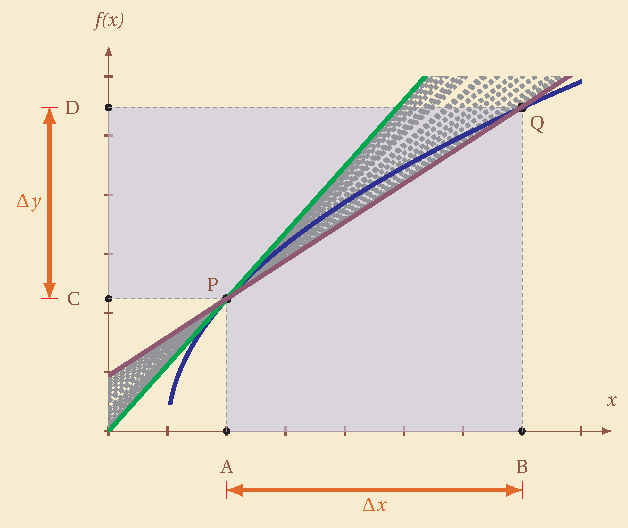
\includegraphics[scale=0.8]{derivada-sec-4.pdf} 
\caption{\protect Aproximaci\'on lineal de $f$ en $c$}
\end{figure}
\begin{equation}
g(x)=f(c)+(x-c)f^{\prime}(c) \label{aproxlinfvsc}%
\end{equation}
(cuya gr\'{a}fica es la ecuaci\'{o}n de la recta tangente en $(c,f(c))$. Ver
figura \ref{difeecni}) es entonces una aproximaci\'{o}n de $f$ en las
vecindades de $c$.
El incremento de $f$ es dado por la
\index{Aplicaci\'{o}n lineal|textbf}%
aplicaci\'{o}n lineal
\begin{equation}
h\longmapsto f^{\prime}(c)h, \label{defdif}%
\end{equation}
la cual es usualmente denominada la \textbf{diferencial%
\index{Diferencial|textbf}%
} de $f$ en $c$.
La existencia de una aplicaci\'{o}n lineal y de una funci\'{o}n de error como
en (\ref{diferencial}) caracteriza a funciones denominadas
\textbf{diferenciables}.
\index{Funciones!-- diferenciables}%
El concepto de diferenciabilidad, para funciones reales de variable real,
coincide as\'{\i} con el de derivabilidad. Por lo tanto $f$ con las
condiciones indicadas en la definici\'{o}n de derivada, se denomina
\textbf{diferenciable%
\index{Funci\'{o}n!-- diferenciable}%
} en $c$ si, y s\'{o}lo si existen una aplicaci\'{o}n lineal%
\[
f_{c}^{\prime}:\rz\longrightarrow\rz,
\]
y una funci\'{o}n
\[
E_{c}:\rz\longrightarrow\rz,
\]
tales que
\begin{align}
f(c+h)  &  =f(c)+f_{c}^{\prime}(h)+E_{c}(h),\label{diferenciabilidadc}\\
\lim_{h\rightarrow0}\frac{E_{c}(h)}{h}  &  =0. \label{errordif}%
\end{align}
La ecuaci\'{o}n (\ref{diferenciabilidadc}) es denominada
\index{F\'{o}rmula de Taylor|textbf}%
\textbf{f\'{o}rmula de Taylor} de primer orden para $f$ en $c$. La funci\'{o}n
$f_{c}^{\prime}$ es la \textbf{diferencial} de $f$ en $c$ citada en
(\ref{defdif}). De la discusi\'{o}n previa se tiene entonces que toda
funci\'{o}n derivable en $x=c,$ es tambi\'{e}n una funci\'{o}n diferenciable
en $x=c$. Rec\'{\i}procamente, si se cumple (\qquad\ref{diferenciabilidadc}) y
(\ref{errordif}), entonces
\begin{align*}
\lim_{h\rightarrow0}\frac{f(c+h)-f(c)}{h}  &  =\lim_{h\rightarrow0}\frac
{f_{c}^{\prime}(h)+Ec(h)}{h}\\
&  =\lim_{h\rightarrow0}\frac{f_{c}^{\prime}(h.1)+E_{c}(h)}{h}\\
&  =\lim_{h\rightarrow0}\frac{hf_{c}^{\prime}(1)+E_{c}(h)}{h}\\
&  =\lim_{h\rightarrow0}\left(  f_{c}^{\prime}(1)+\frac{E_{c}(h)}{h}\right) \\
&  =f_{c}^{\prime}(1),
\end{align*}
lo cual demuestra que $f$ es derivable en $c$ y que
\[
f^{\prime}(c)=f_{c}^{\prime}(1).
\]
Si escribimos $h=x-c$, la derivada puede escribirse tambi\'{e}n como
\begin{equation}
f^{\prime}(c)=\lim_{x\rightarrow c}\frac{f(x)-f(c)}{x-c}.
\end{equation}
Si suponemos $f$ derivable en $x=c,$ es inmediato que
\begin{align*}
\lim_{x\rightarrow c}f(x)  &  =\lim_{x\rightarrow c}\frac{f(x)-f(c)+f(c)}%
{x-c}(x-c)\\
&  =\lim_{x\rightarrow c}\left(  \frac{f(x)-f(c)}{x-c}(x-c)+f(c)\right) \\
&  =f^{\prime}(c)(0)+f(c)\\
&  =f(c)
\end{align*}
y, por lo tanto se cumple el siguiente resultado
\begin{theorem}
\label{d15}Si $f:\left]  a,b\right[  \rightarrow\rz$ es diferenciable%
\index{Funci\'{o}n!-- continua}
en $x=c\in\left]  a,b\right[  $. Entonces $f$ es continua en $x=c$.
\end{theorem}
Ell rec\'{\i}proco es falso en general, como ejemplo tomemeos la funci\'{o}n
valor absoluto
\[
f(x)=|x|,
\]
la cual es continua en $x=0$, pero no es diferenciable en el mismo. En
efecto:
\begin{align*}
\lim_{h\rightarrow0^{+}}\frac{|h|}{h}  &  =1\\
\lim_{h\rightarrow0^{-}}\frac{|h|}{h}  &  =-1,
\end{align*}
por lo que $f^{\prime}(0)$ no existe.

Si consideramos los valores $x$ para quienes exista el l\'{\i}mite
\begin{equation}
f^{\prime}\left(  x\right)  =\lim_{h\rightarrow0}\frac{f\left(  x+h\right)
-f\left(  x\right)  }{h}. \label{d2}%
\end{equation}
\ Entonces se puede asignar a cada $x$ el n\'{u}mero $f^{\prime}\left(
x\right)  $. De esta manera en $\left(  \ref{d2}\right)  $ se define una nueva
funci\'{o}n llamada la derivada de $f$. Si $f^{\prime}$ es continua decimos
que $f$ es
\index{Funci\'{o}n!-- continuamente diferenciable}%
continuamente diferenciable
\begin{notation}
Si $y=f\left(  x\right)  $, la derivada de $f$ respecto a $x$ puede notarse de
cualquiera de las siguientes maneras%
\[
f^{\prime}\left(  x\right)  \equiv y^{\prime}\equiv\dfrac{dy}{dx}\equiv
\dfrac{d}{dx}f\left(  x\right)  \equiv Df\left(  x\right)  \equiv D_{x}f.
\]
\end{notation}
\begin{definition}
[Derivadas laterales]%
\index{Derivadas!laterales}%
Se define la derivada a la derecha (derivada lateral derecha) de $f$ en $x=c$
como $f_{+}^{\prime}$ donde
\[
f_{+}^{\prime}\left(  c\right)  =\lim_{h\rightarrow0^{+}}\frac{f\left(
c+h\right)  -f\left(  c\right)  }{h}\,\,,
\]
si este l\'{\i}mite existe. An\'{a}logamente, se define la derivada a la
izquierda (derivada lateral izquierda) de $f$ en $x=c$ como $f_{-}^{\prime}$
donde
\[
f_{-}^{\prime}\left(  x_{0}\right)  =\lim_{h\rightarrow0^{+}}\frac{f\left(
c+h\right)  -f\left(  c\right)  }{h}\,\,,
\]
si este l\'{\i}mite existe.\newline De la definici\'{o}n de derivada, se puede
decir que una funci\'{o}n $f$ es derivable en $x=c$ si, y solo si
$f_{+}^{\prime}\left(  c\right)  =f_{-}^{\prime}\left(  c\right)  .$
\end{definition}
\begin{definition}
[Diferenciabilidad en un intervalo]%
\index{Derivabilidad!-- en un intervalo}%
Se dice que $f$ es diferenciable en un intervalo abierto $\left]  a,b\right[
$, si $f$ es diferenciable en cada punto del intervalo $\left]  a,b\right[  .$
\end{definition}
Para intervalos de otro tipo, la exigencia de derivabilidad en los extremos se
puede debilitar, exigiendo simplemente derivabilidad lateral en dichos puntos.
Por ejemplo, diremos que $f:[a,b]\rightarrow\rz$ es diferenciable en el
intervalo cerrado $[a,b]$, si $f$ es diferenciable en el intervalo abierto
$\left]  a,b\right[  ,$ y si adem\'{a}s$\ f_{+}^{\prime}\left(  a\right)  \ $y
$\ f_{-}^{\prime}\left(  b\right)  $ existen.
\subsection{Derivada de orden superior}
Si $f:\left]  a,b\right[  \longrightarrow\rz$ es
\index{Derivadas!-- de orden superior}%
una funci\'{o}n, y si $f$ es diferenciable en $c\in\left]  a,b\right[  $,
entonces el conjunto
\[
U=\{x\in\left]  a,b\right[  \mid f^{\prime}(x)\ \mbox{ \ existe}\}
\]
es no vac\'{\i}o. Definimos
\begin{equation}%
\begin{tabular}
[c]{llll}%
$f^{\prime}:$ & $U$ & $\longrightarrow$ & $\rz$\\
& $x$ & $\longmapsto$ & $f^{\prime}\left(  x\right)  .$%
\end{tabular}
\end{equation}
$f^{\prime}$ es la \textbf{funci\'{o}n derivada%
\index{Funci\'{o}n!-- derivada}%
} de $f$ en $U$.

Por lo tanto, si $f$ es una funci\'{o}n diferenciable en un intervalo, su
derivada $f^{\prime}$ puede tambi\'{e}n ser diferenciable, en tal caso su
derivada se denota por $f^{\prime\prime}$. Es decir, la segunda derivada es la
derivada de la derivada . Y as\'{\i} sucesivamente podr\'{\i}amos continuar
derivando para obtener $f^{\prime\prime\prime}=f^{(3)},$ $f^{\prime
\prime\prime\prime}=f^{(4)},\dots.$\newline En general, se puede denotar las
derivadas de orden superior como%
\[
f^{\left(  n\right)  }\left(  x\right)  =y^{\left(  n\right)  }=\frac{d^{n}%
y}{dx^{n}}=\frac{d}{dx}\left(  \frac{d^{n-1}y}{dx^{n-1}}\right)
\ \ ,si\ \ n\geq2
\]
Tambi\'{e}n es usual escribir $C^{n}\left]  a,b\right[  $ para el conjunto de
todas las funciones con derivadas hasta el orden $n$, al menos, y con dichas
derivadas continuas en el intervalo $\left]  a,b\right[  $, $a,b\in\rz$.%
\index{d@$C^{\infty}\left]  a,b\right[  $}
$C^{\infty}\left]  a,b\right[  $ es el conjunto de todas las funciones con
derivadas continuas de todos los ordenes sobre $\left]  a,b\right[  $.
\subsection{Interpretaci\'{o}n geom\'{e}trica de la
derivada\label{ingeodelader}}
De la discusi\'{o}n previa se tiene que en el caso que $f$ sea derivable en
$x=c,$ existe una aproximaci\'{o}n lineal de $f$ en las vecindades de $c$ dada
por (\ref{aproxlinfvsc}). Lo interesante es que esta ecuaci\'{o}n coincide con
la ecuaci\'{o}n de la recta tangente a la gr\'{a}fica de la funci\'{o}n y la
derivada con la pendiente de dicha recta. Para justificar lo anterior,
consideremos la funci\'{o}n $y=f\left(  x\right)  ,$ con $f$ diferenciable en
$x=c$. Observemos que el cociente $\dfrac{f\left(  c+h\right)  -f\left(
c\right)  }{h}$ representa la pendiente de la recta secante que pasa por los
puntos $\left(  c,f\left(  c\right)  \right)  $ y $\left(  c+h,f\left(
c+h\right)  \right)  $ (ver figura \ref{recsec1} )$.$ Al tomar l\'{\i}mite
cuando $h\rightarrow0$,
\index{Derivada!Interpretaci\'{o}n!geom\'{e}trica|textit}%
la pendiente de la recta secante tiende al valor de la
\index{Recta tangente|textbf}%
pendiente de la recta tangente.\ Por lo tanto $f^{\prime}\left(  c\right)  $
es la pendiente de la recta tangente a la curva $y=f\left(  x\right)  $ en el
punto $\left(  c,f\left(  c\right)  \right)  $ y la ecuaci\'{o}n de la recta
tangente es%
\[
y-f\left(  c\right)  =f^{\prime}\left(  c\right)  \left(  x-c\right)
\]
\begin{figure}[H]
\centering
\includegraphics[scale=0.8]%
{derivada-tan.pdf}%
\caption{Tangente a la gr\'{a}fica de una funci\'{o}n }%
\label{recsec1}%
\end{figure}
Como consecuencia se considera,
\begin{definition}
Sea $f$ una funci\'{o}n derivable en $x=c.$ La recta tangente a la gr\'{a}fica
de $f$ en el punto $\left(  c,f\left(  c\right)  \right)  $ es aquella recta
cuya pendiente est\'{a} dada por $f^{\prime}\left(  c\right)  $.
\end{definition}
Observe que esta definici\'{o}n en ning\'{u}n momento excluye la posibilidad
de que la recta tangente corte a la gr\'{a}fica de la funci\'{o}n en varias
ocasiones .
\subsection{Interpretaci\'{o}n f\'{\i}sica de la derivada}
Consideremos una part\'{\i}cula que se mueve a lo largo de una recta durante
un intervalo de tiempo $t_{0}\leq t\leq t_{1}$, con una ecuaci\'{o}n de
posici\'{o}n dada por $x=x\left(  t\right)  $.%
\index{Derivada!Interpretaci\'{o}n!f\'{\i}sica|textit}%
\index{Funci\'{o}n!-- posici\'{o}n}%
Se conoce como velocidad promedio o velocidad media de la part\'{\i}cula en
$\left[  t_{0},t_{1}\right]  ,$ al cociente%
\[
\frac{\Delta x}{\Delta t}=\frac{x\left(  t_{1}\right)  -x\left(  t_{0}\right)
}{t_{1}-t_{0}}:=\overline{v}.
\]
La velocidad media por lo general no brinda informaci\'{o}n sobre la velocidad
de la part\'{\i}cula en un punto cualesquiera $t_{2}\in\left[  t_{0}%
,t_{1}\right]  .$ Si el movimiento es rectilineo uniforme, es claro que para
todo punto en $\left]  t_{0},t_{1}\right[  $, la%
\index{Velocidad!-- promedio}%
\index{Velocidad!-- instantanea}
velocidad de la part\'{\i}cula estar\'{a} dada por $\overline{v}.$ Pero si el
movimiento no es rectilineo uniforme, el problema debe abordarse de otra forma.
Ahora, como el desplazamiento de la part\'{\i}cula en un intervalo $\left[
t_{2},t_{2}+h\right]  $ viene dado por
\[
\Delta x=x\left(  t_{2}+h\right)  -x\left(  t_{2}\right)  .
\]
Entonces, la velocidad media en dicho intervalo estar\'{a} dada por%
\[
\overline{v}=\frac{x\left(  t_{2}+h\right)  -x\left(  t_{2}\right)  }%
{h}=:\overline{v}_{h}\left(  t_{2}\right)  .
\]
A medida que consideramos $h\approx0,$ es claro que se tendran valores de
velocidades medias para instantes cada vez mas cercanos a $t_{2}.$ Extendiendo
este hecho se define la velocidad instantanea de la part\'{\i}cula en
$t=t_{2}$ al l\'{\i}mite (en caso de existir):
\[
v\left(  t_{2}\right)  =\lim_{h\rightarrow0}\overline{v}_{h}\left(
t_{2}\right)  =\lim_{h\rightarrow0}\frac{x\left(  t_{2}+h\right)  -x\left(
t_{2}\right)  }{h}.
\]
Pero en caso de existir el l\'{\i}mite anterior se tiene que $x^{\prime
}\left(  t_{2}\right)  =\lim\limits_{h\rightarrow0}\dfrac{x\left(
t_{2}+h\right)  -x\left(  t_{2}\right)  }{h}.$ Es decir,%
\[
x^{\prime}\left(  t_{2}\right)  =v\left(  t_{2}\right)  .
\]
Por lo tanto, la derivada de la funci\'{o}n posici\'{o}n en el instante
$t=t_{2}$ representa la velocidad instant\'{a}nea de la part\'{\i}cula en
dicho instante.%
\index{Aceleraci\'{o}n!-- media}%
\index{Aceleraci\'{o}n!-- instantanea}%
En forma an\'{a}loga se muestra que la aceleraci\'{o}n instantanea de la
part\'{\i}cula en el instante $t=t_{2}$ esta dado por%
\[
a\left(  t_{2}\right)  =\lim_{h\rightarrow0}\overline{a}_{h}\left(
t_{2}\right)  =\lim_{h\rightarrow0}\frac{v\left(  t_{2}+h\right)  -v\left(
t_{2}\right)  }{h}.
\]
Por lo cual
\[
a\left(  t_{2}\right)  =v^{\prime}\left(  t_{2}\right)  =x^{\prime\prime
}\left(  t_{2}\right)  .
\]
Si consideramos lo expuesto en \ref{ingeodelader}, es claro que en la
gr\'{a}fica $x\left(  t\right)  $ vs. $t,$ la velocidad en el punto $t_{0}$
viene dada por la pendiente de la recta tangente a la curva en $t_{0}$.
An\'{a}logamente, si tenemos la gr\'{a}fica $v\left(  t\right)  $ vs. $t,$ la
aceleraci\'{o}n en $t_{0}\ $es la pendiente de recta tangente a la curva en
$t_{0}.$%
\begin{center}
\includegraphics[scale=0.6]%
{fig-3-4.pdf}%
\end{center}
\section{Teoremas relativos a la derivada.%
\index{Derivada!Teorema relativos de la --}%
}
En esta secci\'{o}n enunciamos sin demostraci\'{o}n algunos teoremas
importantes para el c\'{a}lculo de derivadas.
\begin{theorem}
\label{d3}Si f y g son funciones diferenciables en $\left]  a,b\right[  $,
entonces las funciones $f+g$ ,$f-g$ , $fg$ y $\dfrac{f}{g}$ (con $g\left(
x\right)  \neq0$ ) tambi\'{e}n son diferenciables en $\left]  a,b\right[  $ y
\begin{enumerate}
\item[a.] si $h\left(  x\right)  =f\left(  x\right)  +g\left(  x\right)  $
entonces $h^{\prime}\left(  x\right)  =f^{\prime}\left(  x\right)  +g^{\prime
}\left(  x\right)  .$
\item[b.] si $h\left(  x\right)  =f\left(  x\right)  -g\left(  x\right)  $
entonces $h^{\prime}\left(  x\right)  =f^{\prime}\left(  x\right)  -g^{\prime
}\left(  x\right)  .$
\item[c.] si $h\left(  x\right)  =f\left(  x\right)  g\left(  x\right)  $
entonces $h^{\prime}\left(  x\right)  =f^{\prime}\left(  x\right)  g\left(
x\right)  +f\left(  x\right)  g^{\prime}\left(  x\right)  .$
\item[d.] si $h\left(  x\right)  =\dfrac{f\left(  x\right)  }{g\left(
x\right)  }$ entonces $h^{\prime}\left(  x\right)  =\dfrac{f^{\prime}\left(
x\right)  g\left(  x\right)  -f\left(  x\right)  g^{\prime}\left(  x\right)
}{[g\left(  x\right)  ]^{2}}.$
\end{enumerate}
\end{theorem}
\begin{theorem}
\label{d4}Si $f\left(  x\right)  =cx^{n},\ \ $donde $c$ es una constante y
$n\in\nz$ . Entonces $f^{\prime}\left(  x\right)  =ncx^{n-1}.$
\end{theorem}
\begin{theorem}
\label{d5}Si $f\left(  x\right)  =cx^{r}$ donde $c$ es una constante y
$r\in\rz$. Entonces $f^{\prime}\left(  x\right)  =rcx^{r-1}.$
\end{theorem}
\begin{theorem}
\label{d6}Si $f\left(  x\right)  =c\ \ \forall x\in\left]  a,b\right[  $,
donde c es una constante. Entonces $f^{\prime}\left(  x\right)  =0.$
\end{theorem}
\begin{theorem}
\label{d376} Si $f\left(  x\right)  =\sum_{k=0}^{k=n}a_{k}x^{k}$es una
funci\'{o}n polinomica, se tiene que
\[
f^{\prime}\left(  x\right)  =\sum_{k=1}^{k=n}ka_{k}x^{k-1}.
\]
\end{theorem}
\begin{theorem}
[Derivada de las funciones trigonometricas]%
\index{Derivada!-- de funciones!trigonom\'{e}tricas|textit}%
\label{d7} \textcolor{white}{.}
\begin{enumerate}
\item[a.] Si $f\left(  x\right)  =\operatorname{sen}x$. Entonces $f^{\prime
}\left(  x\right)  =\cos x$.
\item[b.] Si $f\left(  x\right)  =\cos x$. Entonces $f^{\prime}\left(
x\right)  =-\operatorname{sen}x$.
\item[c.] Si $f\left(  x\right)  =\tan x$. Entonces $f^{\prime}\left(
x\right)  =\sec^{2}x$.
\item[d.] Si $f\left(  x\right)  =\cot x$. Entonces $f^{\prime}\left(
x\right)  =-\csc^{2}x$.
\item[e.] Si $f\left(  x\right)  =\sec x$. Entonces $f^{\prime}\left(
x\right)  =\sec x\tan x$.
\item[f.] Si $f\left(  x\right)  =\csc x$. Entonces $f^{\prime}\left(
x\right)  =-\csc x\cot x$.
\end{enumerate}
\end{theorem}
\begin{theorem}
\label{d8}
\index{Regla de la cadena}%
Supongamos que $g$ es diferenciable en $x$, y $f$ es diferenciable en
$g\left(  x\right)  .$ Entonces la funci\'{o}n $h\left(  x\right)  =f\left(
g\left(  x\right)  \right)  $ es diferenciable en $x$ y
\begin{equation}
h^{\prime}\left(  x\right)  =f^{\prime}\left(  g\left(  x\right)  \right)
\cdot g^{\prime}\left(  x\right)  \label{cadena}%
\end{equation}
\end{theorem}
La ecuaci\'{o}n (\ref{cadena}) es denominada usualmente \textbf{regla de la
cadena} para la derivada de funciones compuestas. Si escribimos
$u=f(g(x)),y=g(x)$, entonces $u=f(y)$ y la ecuaci\'{o}n (\ref{cadena}) adopta
la forma
\begin{equation}
\frac{du}{dx}=\frac{du}{dy}\frac{dy}{dx}. \label{cadena2}%
\end{equation}
\begin{theorem}
[Derivada de la funci\'{o}n exponencial y logar\'{\i}tmica]\label{d9}%
\textcolor{white}{.}\label{d7 copy(1)}
\begin{enumerate}
\item[a.] Si $f\left(  x\right)  =\ln x$.%
\index{Derivada!-- de funciones!trascendentes|textit}
Entonces $f^{\prime}\left(  x\right)  =\dfrac{1}{x}$.
\item[b.] Si $f\left(  x\right)  =\ln\left\vert g\left(  x\right)  \right\vert
$. Entonces $f^{\prime}\left(  x\right)  =\dfrac{g^{\prime}\left(  x\right)
}{g\left(  x\right)  }$.
\item[c.] Si $f\left(  x\right)  =\log_{a}x$. Entonces $f^{\prime}\left(
x\right)  =\dfrac{1}{x\ln a}$.
\item[d.] Si $f\left(  x\right)  =e^{x}$. Entonces$\ \ f^{\prime}\left(
x\right)  =e^{x}$.
\item[e.] Si $f\left(  x\right)  =e^{g\left(  x\right)  }$. Entonces
$f^{\prime}\left(  x\right)  =g^{\prime}\left(  x\right)  e^{g\left(
x\right)  }$.
\item[f.] Si $f\left(  x\right)  =a^{x}$ $\left(  a>0,\ a\neq1\right)  $.
Entonces $f^{\prime}\left(  x\right)  =a^{x}\ln a$.
\end{enumerate}
\end{theorem}
\begin{theorem}
[Derivada de la funciones trigonometricas inversas]\label{d10}
\textcolor{white}{.}%
\index{Derivada!-- de funciones!trigonom\'{e}tricas inversas|textit}%
\begin{enumerate}
\item[a.] Si $f\left(  x\right)  =\arcsin x,\left\vert x\right\vert <1$.
Entonces $f^{\prime}\left(  x\right)  =\dfrac{1}{\sqrt{1-x^{2}}}$.
\item[b.] Si $f\left(  x\right)  =\arccos x,\left\vert x\right\vert <1$.
Entonces $f^{\prime}\left(  x\right)  =\dfrac{-1}{\sqrt{1-x^{2}}}$.
\item[c.] Si $f\left(  x\right)  =\arctan x,x\in\left]  -\infty,+\infty
\right[  $. Entonces $f^{\prime}\left(  x\right)  =\dfrac{1}{1+x^{2}}$.
\item[d.] Si $f\left(  x\right)  =\operatorname*{arccot}x,x\in\left]
-\infty,+\infty\right[  $. Entonces $f^{\prime}\left(  x\right)  =-\dfrac
{1}{1+x^{2}}.$
\item[e.] Si $f\left(  x\right)  =\operatorname*{arcsec}x,\left\vert
x\right\vert >1$. Entonces $f^{\prime}\left(  x\right)  =\dfrac{1}{\left\vert
x\right\vert \sqrt{x^{2}-1}}.$
\item Si $f\left(  x\right)  =\operatorname*{arccsc}x,\left\vert x\right\vert
>1.$ Entonces $f^{\prime}\left(  x\right)  =-\dfrac{1}{\left\vert x\right\vert
\sqrt{x^{2}-1}}.$
\end{enumerate}
\end{theorem}
\begin{theorem}
[Regla de L'H\^{o}pital]%
\index{e@Regla de L'H\^{o}pital}%
\label{d11} \textcolor{white}{.} Si f y g son funciones continuamente
diferenciables en el intervalo $I=\left]  a-\delta,a+\delta\right[  ,\delta
>0$, y supongamos que $f\left(  a\right)  =0$, $g\left(  a\right)  =0$ y
$g^{\prime}\left(  x\right)  \neq0$ para $x\neq a\ $. Entonces
\[
\lim\limits_{x\rightarrow a}\dfrac{f\left(  x\right)  }{g\left(  x\right)
}=\lim\limits_{x\rightarrow a}\dfrac{f^{\prime}\left(  x\right)  }{g^{\prime
}\left(  x\right)  }.
\]
\end{theorem}
\section{Derivaci\'{o}n impl\'{\i}cita%
\index{Derivada!-- impl\'{\i}cita}%
}
Si una ecuaci\'{o}n en dos variables define impl\'{\i}citamente una variable
como funci\'{o}n diferenciable de la otra, podemos entonces utilizar la regla
de la cadena para encontrar la derivada de dicha funci\'{o}n. Para ser m\'{a}s
precisos supongamos
\begin{itemize}
\item $F(x,y)=0$ es una ecuaci\'{o}n en las variables $x$ y $y.$
\item $y=f(x)$ est\'{a} definida impl\'{\i}citamente por $F(x,y)=0$, y
\item $f$ es diferenciable en alg\'{u}n abierto $\left]  a,b\right[  $.
\end{itemize}
De los tres items anteriores, tenemos la ecuaci\'{o}n
\index{Funci\'{o}n!-- definida implicitamente}
\[
g(x)=F(x,f(x))=0,
\]
de donde se tiene que $g^{\prime}(x)=0$. Es decir, podemos diferenciar en
ambos miembros y obtener as\'{\i} una ecuaci\'{o}n \textquotedblleft
diferencial\textquotedblright\
\[
\frac{d}{dx}(F(x,y))=G(x,y,y^{\prime})=0
\]
la cual es satisfecha por $f$ y su derivada $f^{\prime}$.
Consideremos, por ejemplo, la ecuaci\'{o}n
\[
x^{2}+y^{2}=1
\]
la cual es la ecuaci\'{o}n de la circunferencia unitaria centrada en $\left(
0,0\right)  $ y, por lo tanto su conjunto soluci\'{o}n no es una funci\'{o}n.
Sin embargo, las ecuaciones:
\begin{align}
y=f(x)  &  =\sqrt{1-x^{2}},\label{unafuncion}\\
y=g(x)  &  =-\sqrt{1-x^{2}} \label{dosfuncion}%
\end{align}
definen funciones impl\'{\i}citas en la ecuaci\'{o}n de la circunferencia.
Para $x\in\left]  -1,1\right[  $, se tiene
\begin{align*}
y^{\prime}=f^{\prime}(x)  &  =-\frac{x}{\sqrt{1-x^{2}}}\\
&  =-\frac{x}{y}\\
y^{\prime}=g^{\prime}(x)  &  =\frac{x}{\sqrt{1-x^{2}}}\\
&  =-\frac{x}{y}%
\end{align*}
N\'{o}tese as\'{\i} que , en ambos casos se satisface la ecuaci\'{o}n
diferencial
\[
y^{\prime}=-\frac{x}{y}.
\]
Esta \'{u}ltima ecuaci\'{o}n se pudo obtener por derivaci\'{o}n
impl\'{\i}cita; es decir, directamente de la ecuaci\'{o}n de la
circunferencia, derivando, respecto a $x$, t\'{e}rmino a t\'{e}rmino y miembro
a miembro en dicha ecuaci\'{o}n, como se muestra a continuaci\'{o}n,
\begin{align*}
\frac{d}{dx}(x^{2}+y^{2})  &  =\frac{d}{dx}(1)\\
2x+2yy^{\prime}  &  =0\\
y^{\prime}  &  =-\frac{x}{y}.
\end{align*}
\subsection{Derivada de la funci\'{o}n inversa%
\index{Derivada!-- de funciones!inversas|textit}%
}
Si $f:\left]  a,b\right[  \in\rz$ es una funci\'{o}n invertible y
diferenciable, con inversa $f^{-1}:\operatorname*{Ran}(f)\longrightarrow
\left]  a,b\right[  $, entonces
\[
f\circ f^{-1}=Id_{\operatorname*{Ran}(f)}%
\]
es diferenciable. Si $f^{-1}$ es diferenciable \footnote{Puede demostrarse que
funciones con derivada no nula en un punto son uno-a-uno en alguna vecindad de
dicho punto y que la inversa es diferenciable en la im\'{a}gen de dicho
punto.} la regla de la cadena produce
\begin{align*}
(f\circ f^{-1})^{\prime}(x)  &  =1\\
f^{\prime}(f^{-1}(x))(f^{-1})^{\prime}(x)  &  =1
\end{align*}
de donde se sigue que
\begin{equation}
(f^{-1})^{\prime}(x)=\frac{1}{f^{\prime}(f^{-1}(x))}
\label{derivadadeinversas}%
\end{equation}
En general, si escribimos $y=f^{-1}(x)$, por definici\'{o}n de inversa se
tiene que
\[
x=f(y).
\]
Derivando con relaci\'{o}n a $x$ y usando la regla de la cadena, tenemos:
\begin{align*}
\frac{d}{dx}(x)  &  =\frac{d}{dx}(f(y))\\
1  &  =f^{\prime}(y)\frac{dy}{dx}\\
\frac{dy}{dx}  &  =\frac{1}{f^{\prime}(y)}\\
&  =\frac{1}{\frac{dx}{dy}}%
\end{align*}
\subsection{Derivaci\'{o}n logar\'{\i}tmica}%
\index{Derivaci\'{o}n!-- logaritmica}%
Si $x\in\rz$, $x\neq0$, entonces $\ln(|x|)$ est\'{a} definido. Si consideramos
la funci\'{o}n
\[
g(x)=\ln(|x|)
\]
con dominio $\rz-\{0\}$, entonces $g$ es una compuesta de funciones
diferenciables en el dominio indicado. Tenemos
\begin{align*}
g^{\prime}(x)  &  =\frac{1}{|x|}\frac{d}{dx}\left(  |x|\right) \\
&  =\frac{1}{|x|}\frac{x}{|x|}\\
&  =\frac{1}{x}%
\end{align*}
Si $r\in\qz$, y $y=x^{r},x>0$, tenemos entonces que
\begin{align*}
\ln(y)  &  =\ln(x^{r})\\
&  =r\ln(x)
\end{align*}
de donde
\begin{align*}
\frac{1}{y}y^{\prime}  &  =r\frac{1}{x}\\
y^{\prime}  &  =ry\frac{1}{x}\\
&  =rx^{r-1}%
\end{align*}
lo que muestra que la regla para la derivada de potencias enteras de $x$ se
extiende a potencias con exponentes racionales. El proceso mostrado en el
c\'{a}lculo de la derivada $y^{\prime}$ es a menudo conocido como
derivaci\'{o}n logar\'{\i}tmica.
\section{Ejercicios resueltos.}
En esta secci\'{o}n se presentan una serie de ejemplo resueltos de c\'{a}lculo
de derivadas de funciones elementales.
\begin{example}
Calcule la derivada de la funci\'{o}n $y=3x^{2}$ utilizando la definici\'{o}n.
\end{example}
\begin{sol}
Tomando $f\left(x\right)=3x^{2}$, es claro que $f\left(x+h\right)
=3(x+h)^{2}$ por lo cual%
\begin{align*}
f^{\prime}(x)=\lim_{h\rightarrow0}\frac{f\left(  x+h\right)  -f\left(
x\right)  }{h}  &  =\lim_{h\rightarrow0}\frac{3\left(  x+h\right)  ^{2}%
-3x^{2}}{h}\\
&  =\lim_{h\rightarrow0}\frac{3x^{2}+6xh+h^{2}-3x^{2}}{h}\\
&  =\lim_{h\rightarrow0}\frac{6xh+h^{2}}{h}=\lim_{h\rightarrow0}\frac{h\left(
6x+h\right)  }{h}\\
&  =\lim_{h\rightarrow0}\left(  6x+h\right)  =6x.
\end{align*}
Entonces, la derivada de $f\left(  x\right)  =3x^{2}$ es $f^{\prime}\left(
x\right)  =6x$.
\end{sol}
\begin{example}
Calcular la derivada de la funci\'{o}n $y=\sqrt{x}$ utilizando la
definici\'{o}n de derivada
\end{example}
\begin{sol}
Como $f\left(x\right)=\sqrt{x}$, se tiene que $f\left(x+h\right)
=\sqrt{x+h}.$ Entonces%
\begin{align*}
f^{\prime}\left(  x\right)   &  =\lim_{h\rightarrow0}\frac{f\left(
x+h\right)  -f\left(  x\right)  }{h}=\lim_{h\rightarrow0}\frac{\sqrt{\left(
x+h\right)  }-\sqrt{x}}{h}\\
&  =\lim_{h\rightarrow0}\frac{\sqrt{\left(  x+h\right)  }-\sqrt{x}}{h}%
\cdot\frac{\sqrt{\left(  x+h\right)  }+\sqrt{x}}{\sqrt{\left(  x+h\right)
}+\sqrt{x}}\\
&  =\lim_{h\rightarrow0}\frac{\left(  x+h\right)  -x}{h\left(  \sqrt{\left(
x+h\right)  }+\sqrt{x}\right)  }=\lim_{h\rightarrow0}\frac{h}{h\left(
\sqrt{\left(  x+h\right)  }+\sqrt{x}\right)  }\\
&  =\lim_{h\rightarrow0}\frac{1}{\sqrt{\left(  x+h\right)  }+\sqrt{x}}%
=\frac{1}{2\sqrt{x}}.
\end{align*}
Por lo tanto, la derivada de $f\left(  x\right)  =\sqrt{x}$ esta dada por
$f^{\prime}\left(  x\right)  =\dfrac{1}{2\sqrt{x}}.$
\end{sol}
\begin{example}
Calcular la derivada de la funci\'{o}n $y=\dfrac{1}{x}$ utilizando la
definici\'{o}n de derivada.
\end{example}
\begin{sol}
En forma similar a los problemas anteriores, calculemos $\lim
\limits_{h\rightarrow0}\dfrac{f\left(  x+h\right)  -f\left(  x\right)  }{h}.$%
\begin{align*}
\lim\limits_{h\rightarrow0}\dfrac{f\left(  x+h\right)  -f\left(  x\right)
}{h}  &  =\lim\limits_{h\rightarrow0}\dfrac{\dfrac{1}{x+h}-\dfrac{1}{x}}{h}\\
&  =\lim\limits_{h\rightarrow0}\dfrac{\dfrac{x-\left(  x+h\right)  }{\left(
x+h\right)  x}}{h}=\lim\limits_{h\rightarrow0}\dfrac{-h}{hx\left(  x+h\right)
}\\
&  =\lim\limits_{h\rightarrow0}\frac{-1}{x\left(  x+h\right)  }=\frac
{-1}{x^{2}}.
\end{align*}
Es decir, la derivada de $f\left(  x\right)  =\dfrac{1}{x}$ es $f^{\prime
}\left(  x\right)  =-\dfrac{1}{x^{2}}.$
\end{sol}
\begin{example}
Calcular la derivada de la funci\'{o}n%
\[
f\left(  x\right)  =20x^{4}-5x^{3}+2x^{2}-5.
\]
\end{example}
\begin{sol}
Usando el teorema \ref{d376} se tiene que%
\[
f^{\prime}\left(x\right)  =80x^{3}-15x^{2}+4x
\]
\end{sol}
\begin{example}
Calcular la derivada de la funci\'{o}n
\[
f\left(x\right)  =\left(6x^{2}+5\right)  \left(x^{3}-3x\right)^{9}.
\]
\end{example}
\begin{sol}
Derivando como un producto y aplicando la regla de la cadena para derivar el
segundo factor se tiene que%
\begin{align*}
f^{\prime}\left(  x\right)   &  =(6x^{2}+5)^{\prime}\cdot\left(
x^{3}-3x\right)  ^{9}+(6x^{2}+5)\cdot\left(  \left(  x^{3}-3x\right)
^{9}\right)  ^{\prime}\\
f^{\prime}\left(  x\right)   &  =\left(  12x\right)  \left(  x^{3}-3x\right)
^{9}+\left(  6x^{2}+5\right)  9\left(  x^{3}-3x\right)  ^{8}\underset{\frac
{d}{dx}\left(  x^{3}-3x\right)  }{\underbrace{\left(  3x^{2}-3\right)  }}\\
&  =3x^{8}\left(  58x^{4}-21x^{2}-45\right)  \left(  x^{2}-3\right)  ^{8}.
\end{align*}
\end{sol}
\begin{example}
Calcular la derivada de la funci\'{o}n
\[
f\left(  x\right)  =\frac{6x^{3}+1}{5x^{2}+3x-4}.
\]
\end{example}
\begin{sol}
Ya que la funci\'{o}n es racional, usando los teoremas \ref{d3}, \ref{d4} y
\ref{d6} se tiene que%
\begin{align*}
f^{\prime}\left(  x\right)   &  =\frac{18x^{2}\left(  5x^{2}+3x-4\right)
-\left(  6x^{3}+1\right)  \left(  10x+3\right)  }{\left(  5x^{2}+3x-4\right)
^{2}}\\
&  =\frac{30x^{4}+36x^{3}-72x^{2}-10x-3}{\left(  5x^{2}+3x-4\right)  ^{2}}.
\end{align*}
\end{sol}
\begin{example}
Calcular la derivada de la funci\'{o}n
\[
f\left(  x\right)  =\frac{x\operatorname{sen}x}{\operatorname{sen}x+\cos x}%
\]
\end{example}
\begin{sol}
Los teoremas \ref{d3}, \ref{d4}, \ref{d6} y \ref{d7} implican que%
\begin{align*}
f^{\prime}\left(  x\right)   &  =\frac{\left(  \operatorname{sen}x+x\cos
x\right)  \left(  \operatorname{sen}x+\cos x\right)  -\left(
x\operatorname{sen}x\right)  \left(  \cos x-\operatorname{sen}x\right)
}{\left(  \operatorname{sen}x+\cos x\right)  ^{2}}\\
&  =\frac{\operatorname{sen}x\cos x+1+x-\cos^{2}x}{\left(  \operatorname{sen}%
x+\cos x\right)  ^{2}}.
\end{align*}
\end{sol}
\begin{example}
Sea%
\[
f\left(  x\right)  =\tan\left(  x^{2}\right)  +\cot\left(  2x\right)  +x^{2}%
\]
Hallar $f^{\prime}\left(  1\right)  \ y$ $f^{\prime}\left(  3\right)  .$
\end{example}
\begin{sol}
Calculemos $f^{\prime}\left(  x\right)  .$ Utilizando los teoremas \ref{d3},
\ref{d5}, \ref{d7} y \ref{d8} se tiene que%
\[
f^{\prime}\left(  x\right)  =2x\sec^{2}\left(  x^{2}\right)  -2\csc^{2}\left(
2x\right)  +2x.
\]
Por lo tanto%
\begin{align*}
f^{\prime}\left(  1\right)   &  =2\sec^{2}\left(  1\right)  -2\csc^{2}\left(
2\right)  +2\approx6.432\\
f^{\prime}\left(  3\right)   &  =6\sec^{2}\left(  9\right)  -2\csc^{2}\left(
6\right)  +6\approx-12.389.
\end{align*}
\end{sol}
\begin{example}
Calcular la derivada de la funci\'{o}n
\[
f\left(  x\right)  =\sqrt{x^{2}+5x+1}%
\]
\end{example}
\begin{sol}
Como $f\left(  x\right)  =\left(  x^{2}+5x+1\right)  ^{%
%TCIMACRO{\U{bd}}%
%BeginExpansion
\frac12
%EndExpansion
}$ los teoremas \ref{d3}, \ref{d4}, \ref{d6}, \ref{d8} implican que%
\begin{align*}
f^{\prime}\left(  x\right)   &  =\frac{1}{2}\left(  x^{2}+5x+1\right)  ^{-%
%TCIMACRO{\U{bd}}%
%BeginExpansion
\frac12
%EndExpansion
}\left(  2x+5\right) \\
&  =\frac{2x+5}{2\sqrt{x^{2}+5x+1}}%
\end{align*}
\end{sol}
\begin{example}
Hallar la segunda derivada de la funci\'{o}n%
\[
f\left(  x\right)  =\frac{x^{2}+4x-1}{x^{2}+x-4}%
\]
\end{example}
\begin{sol}
Calculemos $f^{\prime}\left(  x\right)  $ y seguidamente $f^{\prime\prime
}\left(  x\right)  $%
\begin{align*}
f^{\prime}\left(  x\right)   &  =\frac{\left(  2x+4\right)  \left(
x^{2}+x-4\right)  -\left(  x^{2}+4x-1\right)  \left(  2x+1\right)  }{\left(
x^{2}+x-4\right)  ^{2}}\\
&  =\frac{-3\left(  x^{2}+2x+5\right)  }{\left(  x^{2}+x-4\right)  ^{2}}%
\end{align*}
y como $f^{\prime\prime}=\left(  f^{\prime}\right)  ^{\prime}$
\begin{align*}
f^{\prime\prime}\left(  x\right)   &  =\frac{-3\left(  2x+2\right)  \left(
x^{2}+x-4\right)  ^{2}+\left(  3x^{2}+6x+15\right)  2\left(  x^{2}+x-4\right)
\left(  2x+1\right)  }{\left(  x^{2}+x-4\right)  ^{4}}\\
&  =\frac{6\left(  x^{2}+x-4\right)  \left(  x^{3}+3x^{2}+15x+9\right)
}{\left(  x^{2}+x-4\right)  ^{4}}=\frac{6\left(  x^{3}+3x^{2}+15x+9\right)
}{\left(  x^{2}+x-4\right)  ^{3}}%
\end{align*}
\end{sol}
\begin{example}
[Existencia de tangentes verticales.]%
\index{Recta tangente!-- vertical}%
Sea $f\left(  x\right)  =\left(  x-2\right)  ^{\frac{1}{3}}.$ Pruebe que la
funci\'{o}n es continua en $x=2,$ pero no diferenciable en dicho punto.
\end{example}
\begin{sol}
La continuidad de $f$ en $x=2$ es inmediata, debido a que
\[
\lim_{x\rightarrow2^{-}}\left(  x-2\right)  ^{\frac{1}{3}}=\lim_{x\rightarrow
2^{+}}\left(  x-2\right)  ^{\frac{1}{3}}=0=f\left(  2\right)  .
\]
Veamos que $f$ no es derivable en $x=2.$ En efecto, se tiene que
\begin{align*}
f^{\prime}\left(  2\right)   &  =\lim_{x\rightarrow2}\frac{f\left(  x\right)
-f\left(  2\right)  }{x-2}\\
&  =\lim_{x\rightarrow2}\frac{\left(  x-2\right)  ^{\frac{1}{3}}-0}{x-2}%
=\lim_{x\rightarrow2}\frac{1}{\left(  x-2\right)  ^{\frac{2}{3}}}=+\infty.
\end{align*}
Se observa que la gr\'{a}fica de $f\left(  x\right)  =\left(  x-2\right)
^{\frac{1}{3}},$ posee una tangente vertical en $x=2$.%
\begin{center}
\includegraphics[scale=0.8]%
{ejr-3-4-11.pdf}%
\end{center}
\end{sol}
\begin{example}
[Existencia de puntos angulosos I]%
\index{Puntos angulosos|textbf}%
Sea
\[
f\left(  x\right)  =\left\{
\begin{array}
[c]{ccc}%
1-x^{2} & \text{\emph{, si}} & x\leq1\\
x-1 & \text{\emph{, si}} & x>1
\end{array}
\right.
\]
Pruebe que la funci\'{o}n es continua en $x=1,$ pero no diferenciable en dicho punto.
\end{example}
\begin{sol}
Como
\[
\lim_{x\rightarrow1^{-}}f\left(  x\right)  =\lim_{x\rightarrow1^{-}}\left(
1-x^{2}\right)  =0=f\left(  1\right)  ,
\]
y
\[
\lim_{x\rightarrow1^{+}}f\left(  x\right)  =\lim_{x\rightarrow1^{+}}\left(
x-1\right)  =0=f\left(  1\right)  .
\]
Entonces $f$ es continua en $x=1.$
Pero
\begin{align*}
f_{-}^{\prime}\left(  1\right)   &  =\lim_{x\rightarrow1^{-}}\frac{f\left(
x\right)  -f\left(  1\right)  }{x-1}\\
&  =\lim_{x\rightarrow1^{-}}\frac{\left(  1-x^{2}\right)  -0}{x-1}\\
&  =-2
\end{align*}
y%
\begin{align*}
f_{+}^{\prime}\left(  1\right)   &  =\lim_{x\rightarrow1^{+}}\frac{f\left(
x\right)  -f\left(  1\right)  }{x-1}\\
&  =\lim_{x\rightarrow1^{+}}\frac{x-1-0}{x-1}\\
&  =1.
\end{align*}
Por lo anterior,
\[
f_{-}^{\prime}\left(  1\right)  \neq f_{+}^{\prime}\left(  1\right)
\]
es decir $\ f$ no es derivable.
Observe que en $x=1$, la funci\'{o}n presenta una esquina o un \'{a}ngulo.%
\begin{center}
\includegraphics[width=0.5\textwidth,height=6cm]%
{ejr-3-4-12.pdf}%
\end{center}
\end{sol}
\begin{example}
[Existencia de puntos angulosos II]Sea
\[
f\left(  x\right)  =\sqrt{\left\vert x\right\vert }%
\]
Pruebe que la funci\'{o}n es continua en $x=0,$ pero no diferenciable en dicho punto.
\end{example}
\begin{sol}
Como
\[
\lim_{x\rightarrow0^{-}}f\left(  x\right)  =\lim_{x\rightarrow0^{-}}\sqrt
{-x}=0=f\left(  0\right)  ,
\]
y
\[
\lim_{x\rightarrow0^{+}}f\left(  x\right)  =\lim_{x\rightarrow0^{+}}\sqrt
{x}=0=f\left(  0\right)  .
\]
Entonces $f$ es continua en $x=0.$
Pero
\begin{align*}
f_{-}^{\prime}\left(  0\right)   &  =\lim_{x\rightarrow0^{-}}\frac{f\left(
x\right)  -f\left(  0\right)  }{x-0}\\
&  =\lim_{x\rightarrow0^{-}}\frac{\sqrt{-x}}{x}=\lim_{x\rightarrow0^{-}%
}-\left(  \frac{\sqrt{-x}}{-x}\right) \\
&  =-\lim_{x\rightarrow0^{-}}\left(  \frac{1}{\sqrt{-x}}\right)  =-\infty.
\end{align*}
y%
\begin{align*}
f_{+}^{\prime}\left(  0\right)   &  =\lim_{x\rightarrow0^{+}}\frac{f\left(
x\right)  -f\left(  0\right)  }{x-0}\\
&  =\lim_{x\rightarrow0^{+}}\frac{\sqrt{x}}{x}\\
&  =\lim_{x\rightarrow0^{+}}\left(  \frac{1}{\sqrt{x}}\right)  =+\infty.
\end{align*}
Por lo anterior, ninguna de las dos derivadas parciales exiten, lo que
trivialmente implica la no derivabilidad de la funci\'{o}n en $x=0$.
Observe que en $x=0$, la funci\'{o}n presenta una c\'{u}spide.%
\begin{center}
\includegraphics[scale=0.8]%
{ejr-3-4-13.pdf}%
\end{center}
\end{sol}
\begin{example}
Hallar la ecuaci\'{o}n de la recta tangente a la curva $f\left(  x\right)
=3x^{2}+5x-10$ en el punto $x=2$.
\end{example}
\begin{sol}
La pendiente $m$ de la recta tangente es la derivada de la funci\'{o}n en el
punto $x=2$.\newline Como $f^{\prime}\left(  x\right)  =6x+5$, se tiene que
$f^{\prime}\left(  2\right)  =17,$ y ya que $f\left(  2\right)  =3\left(
2\right)  ^{2}+5\left(  2\right)  -10=12$, se tiene que la ecuaci\'{o}n de la
recta tangente, viene dada por%
\begin{align*}
y-f\left(  2\right)   &  =m\left(  x-2\right) \\
y-12  &  =17\left(  x-2\right) \\
y  &  =17x-22
\end{align*}
Este resultado lo podemos confirmar observado las gr\'{a}ficas de las
funciones $f\left(  x\right)  =3x^{2}+5x-10$ y de $g\left(  x\right)  =17x-22$
que se presentan a continuaci\'{o}n%
\begin{center}
\includegraphics[scale=0.4]%
{ejr-3-4-14.pdf}%
\end{center}
\end{sol}
\begin{example}
Hallar la ecuaci\'{o}n de las rectas tangentes a la circunferencia%
\begin{equation}
x^{2}+y^{2}-2x-4y-20=0 \label{d12}%
\end{equation}
en el punto $x=4$.
\end{example}
\begin{sol}
Para calcular la derivada $y\prime$, utilicemos el m\'{e}todo de la
derivaci\'{o}n impl\'{\i}cita.%
\begin{align*}
2x+2yy^{\prime}-2-4y^{\prime}  &  =0\\
2yy^{\prime}-4y^{\prime}  &  =2-2x\\
y^{\prime}  &  =\frac{2-2x}{2y-4}%
\end{align*}
Como el valor de la pendiente de la recta tangente en un punto est\'{a} dado
por el valor de la derivada en dicho punto, necesitamos encontrar el valor de
$y$ cuando $x=4;$ para ello reemplazando en (\ref{d12}) se obtiene que%
\begin{align*}
16+y^{2}-8-4y-20  &  =0\implies y^{2}-4y-12=0\\
\left(  y+2\right)  \left(  y-6\right)   &  =0\implies y=-2\vee\text{ }y=6
\end{align*}
entonces el valor de las pendientes de las rectas tangentes a la
circunferencia en los puntos $\left(  4,6\right)  $ y $\left(  4,-2\right)  $
estan dadas por:
\[
m_{1}=y\prime\left(  4,6\right)  =\dfrac{2-2\left(  4\right)  }{2\left(
6\right)  -4}=-\dfrac{3}{4}\ \ \ \text{y}\ \ \ m_{2}=y\prime\left(
4,-2\right)  =\dfrac{2-2\left(  4\right)  }{2\left(  -2\right)  -4}=\dfrac
{3}{4}%
\]
Por lo tanto, las ecuaciones de la recta tangentes en los puntos $\left(
4,6\right)  \ y\ \left(  4,-2\right)  $ son%
\[
y=-\frac{3}{4}\left(  x-4\right)  +6\ \ \ \ \ \ \ \text{y}%
\ \ \ \ \ \ \ \ y=\frac{3}{4}\left(  x-4\right)  -2
\]
Este resultado lo podemos confirmar observando las graficas de las funciones
$x^{2}+y^{2}-2x-4y-20=0,\ \ y=-\frac{3}{4}\left(  x-4\right)  +6,\ $%
\ $y=\frac{3}{4}\left(  x-4\right)  -2$ dadas en la figura siguiente.%

\begin{center}
\includegraphics[scale=0.6]%
{ejr-3-4-15.pdf}%
\end{center}

\end{sol}
\begin{example}
Calcular la derivada de la funci\'{o}n%
\[
f\left(  x\right)  =\ln\left(  \cos2x+\operatorname{sen}2x\right)
\]
\end{example}
\begin{sol}
Aplicando el teorema \ref{d9} se tiene%
\[
f^{\prime}\left(  x\right)  =\frac{-2\operatorname{sen}2x+2\cos x}%
{\cos2x+\operatorname{sen}2x}%
\]
\end{sol}
\begin{example}
Calcular la derivada de la funci\'{o}n%
\[
f\left(  x\right)  =\ln\frac{x^{2}+1}{x^{2}-1}%
\]
\end{example}
\begin{sol}
Ya que para $a,b\in\rz^{+},\ln\frac{a}{b}=\ln a-\ln b$ se tiene que
\[
f\left(  x\right)  =\ln\frac{x^{2}+1}{x^{2}-1}=\ln\left(  x^{2}+1\right)
-\ln\left(  x^{2}-1\right)  .
\]
Al derivar se obtiene que:
\[
f^{\prime}\left(  x\right)  =\frac{2x}{x^{2}+1}-\frac{2x}{x^{2}-1}=\frac
{-4x}{\left(  x^{2}+1\right)  \left(  x^{2}-1\right)  }.
\]
\end{sol}
\begin{example}
Calcular la derivada de la funci\'{o}n%
\[
f\left(  x\right)  =\ln\sqrt[3]{\frac{x+1}{x-1}}%
\]
\end{example}
\begin{sol}
Aplicando las propiedades del logaritmo y derivando se tiene%
\begin{align*}
f\left(  x\right)   &  =\frac{1}{3}\ln\frac{x+1}{x-1}=\frac{1}{3}\ln\left(
x+1\right)  -\frac{1}{3}\ln\left(  x-1\right) \\
f^{\prime}\left(  x\right)   &  =\frac{1}{3\left(  x+1\right)  }-\frac
{1}{3\left(  x-1\right)  }=-\frac{2}{3\left(  x+1\right)  \left(  x-1\right)
}.
\end{align*}
\end{sol}
\begin{example}
Calcular la derivada de la funci\'{o}n%
\[
f\left(  x\right)  =e^{x}\operatorname{sen}\left(  e^{x}\right)
\]
\end{example}
\begin{sol}
Aplicando el teorema \ref{d3} (derivada de un producto) se tiene que%
\begin{align*}
f^{\prime}\left(  x\right)   &  =e^{x}\operatorname{sen}\left(  e^{x}\right)
+e^{x}\cos\left(  e^{x}\right)  e^{x}\\
&  =e^{x}\operatorname{sen}\left(  e^{x}\right)  +e^{2x}\cos\left(
e^{x}\right)
\end{align*}
\end{sol}
\begin{example}
Aplicando derivaci\'{o}n logaritmica%
\index{Derivaci\'{o}n!-- logaritmica}%
, determine la derivada de la funci\'{o}n
\[
f\left(  x\right)  =(3x+2)^{x+1},\ x>\frac{-2}{3}%
\]
\end{example}
\begin{sol}
Aplicando derivaci\'{o}n logaritmica se tiene que,%
\begin{align*}
\ln(|y|)  &  =(x+1)\ln(|3x+2|)\\
\frac{1}{y}y^{\prime}  &  =(x+1)\frac{3}{3x+2}+\ln(3x+2)\\
y^{\prime}  &  =(3x+2)^{x+1}\left(  \frac{3(x+1)}{3x+2}+\ln(3x+2)\right) \\
&  =3(x+1)(3x+2)^{x}+(3x+2)^{x+1}\ln(3x+2)
\end{align*}
\end{sol}
\begin{example}
Calcular la derivada de la funci\'{o}n%
\[
f\left(  x\right)  =x^{x}+xe^{\operatorname{sen}x}%
\]
\end{example}
\begin{sol}
Aplicando derivaci\'{o}n logaritmica al primer sumando del miembro derecho se
tiene que
\begin{align*}
y  &  =x^{x}\\
\ln y  &  =x\ln x
\end{align*}
derivando a ambos lados la \'{u}ltima ecuaci\'{o}n, se obtiene $\dfrac
{y^{\prime}}{y}=\ln x+1$. Por lo tanto,%
\[
y^{\prime}=x^{x}\left(  \ln x+1\right)
\]
entonces
\begin{align*}
f\left(  x\right)   &  =x^{x}+xe^{\operatorname{sen}x}\\
f^{\prime}\left(  x\right)   &  =\left(  1+\ln x\right)  x^{x}%
+e^{\operatorname{sen}x}+x\left(  \cos x\right)  e^{\operatorname{sen}x}\\
&  =\left(  1+\ln x\right)  x^{x}+e^{\operatorname{sen}x}+x\left(  \cos
x\right)  e^{\operatorname{sen}x}.
\end{align*}
De igual forma, observe que:
\[
y=x^{x}\implies\ln y=x\ln x\implies y=e^{x\ln x},
\]
de donde,%
\[
x^{x}=e^{x\ln x}%
\]
entonces
\begin{align*}
f\left(  x\right)   &  =e^{x\ln x}+xe^{\sin x}\\
f^{\prime}\left(  x\right)   &  =\left(  1+\ln x\right)  e^{x\ln x}+e^{\sin
x}+x\left(  \cos x\right)  e^{\sin x}\\
&  =\left(  1+\ln x\right)  x^{x}+e^{\sin x}+x\left(  \cos x\right)  e^{\sin
x}%
\end{align*}
\end{sol}
\begin{example}
Calcular la derivada de la funci\'{o}n%
\[
f\left(  x\right)  =\ln\left(  \frac{e^{4x}-1}{e^{4x}+1}\right)
\]
\end{example}
\begin{sol}
Aplicando la propiedades del logaritmo y derivando se tiene%
\begin{align*}
f\left(  x\right)   &  =\ln\left(  e^{4x}-1\right)  -\ln\left(  e^{4x}%
+1\right) \\
f^{\prime}\left(  x\right)   &  =\frac{4e^{4x}}{e^{4x}-1}-\frac{4e^{4x}%
}{e^{4x}+1}=\frac{8e^{4x}}{\left(  e^{4x}-1\right)  \left(  e^{4x}+1\right)  }%
\end{align*}
\end{sol}
\begin{example}
Dada la ecuaci\'{o}n
\[
x^{2}y^{2}=x^{2}+y^{2}.
\]
Aplicar el m\'{e}todo de la derivaci\'{o}n impl\'{\i}cita para hallar la
derivada $y\prime$.
\end{example}
\begin{sol}
Como $x^{2}y^{2}=x^{2}+y^{2}$ se tiene que%
\begin{align*}
(x^{2}y^{2})^{\prime}  &  =(x^{2}+y^{2})^{\prime}\\
2xy^{2}+x^{2}\left(  2yy^{\prime}\right)   &  =2x+2yy^{\prime}\\
2x^{2}yy^{\prime}-2yy^{\prime}  &  =2x-2xy^{2}\\
2yy^{\prime}\left(  x^{2}-1\right)   &  =2x\left(  1-y^{2}\right) \\
y^{\prime}  &  =\frac{x\left(  1-y^{2}\right)  }{y\left(  x^{2}-1\right)  }%
\end{align*}
\end{sol}
\begin{example}
Dada la ecuaci\'{o}n
\[
x\operatorname{sen} y+y\cos x=1.
\]
halle la derivada $y\prime$.
\end{example}
\begin{sol}
Aplicando el m\'{e}todo de la derivaci\'{o}n impl\'{\i}cita se tiene:%
\begin{align*}
(x\operatorname{sen} y+y\cos x)^{\prime}  &  =(1)^{\prime}\\
\operatorname{sen} y+x\left(  \cos y\right)  y^{\prime}+y^{\prime}\cos
x-y\operatorname{sen} x  &  =0\\
xy^{\prime}\cos y+y^{\prime}\cos x  &  =-\operatorname{sen}
y+y\operatorname{sen} x\\
y^{\prime}\left(  x\cos y+\cos x\right)   &  =-\operatorname{sen}
y+y\operatorname{sen} x\\
y^{\prime}  &  =\frac{-\operatorname{sen} y+y\operatorname{sen} x}{x\cos
y+\cos x}%
\end{align*}
\end{sol}
\begin{example}
Dada la ecuaci\'{o}n
\[
3x^{2}+4y^{2}=12
\]
Aplicar el m\'{e}todo de la derivaci\'{o}n impl\'{\i}cita para hallar
$y^{\prime\prime}$.
\end{example}
\begin{sol}
Derivando impl\'{\i}citamente se tiene que,%
\[
6x+8yy^{\prime}=0.\,\,\hbox{Es decir,}\,\,y^{\prime}=\frac{-3x}{4y}.
\]
Derivando nuevamente obtenemos:
\[
6+8\left(  y^{\prime}\right)  ^{2}+8yy^{\prime\prime}%
=0.\,\,\hbox{Por lo tanto,}\,\,y^{\prime\prime}=\frac{-6-8\left(  y^{\prime
}\right)  ^{2}}{8y}.
\]
Reemplazando $y^{\prime}$ en la ecuaci\'{o}n anterior, esta toma la forma
\[
y^{\prime\prime}=\frac{-6-8\left(  \frac{-3x}{4y}\right)  ^{2}}{8y}=-\frac
{3}{16}\frac{\left(  3x^{2}+4y^{2}\right)  }{y^{3}}.
\]
Es decir,
\[
y^{\prime\prime}=\frac{-9}{4y^{3}}.
\]
\end{sol}
\begin{example}
Calcular
\[
\lim_{x\rightarrow1}\frac{x^{4}-5x^{3}+2x^{2}-7x+9}{x^{3}+x^{2}-x-1}.
\]
\end{example}
\begin{sol}
Observe que el l\'{\i}mite dado presenta la forma indeterminada $\frac{0}{0}$,
por lo tanto aplicamos la regla del L'H\^{o}pital, teorema \ref{d11}, con la
cual se tiene que,%
\begin{align*}
\lim_{x\rightarrow1}\frac{x^{4}-5x^{3}+2x^{2}-7x+9}{x^{3}+x^{2}-x-1}  &  =
\lim_{x\rightarrow1}\frac{(x^{4}-5x^{3}+2x^{2}-7x+9)^{\prime}}{(x^{3}%
+x^{2}-x-1)^{\prime}}\\
&  =\lim_{x\rightarrow1}\frac{4x^{3}-15x^{2}+4x-7}{3x^{2}+2x-1}\\
&  =\frac{-7}{2}%
\end{align*}
\end{sol}
\begin{example}
Calcular el l\'{\i}mite.%
\[
\lim_{x\rightarrow0}\frac{x-\operatorname{sen} x}{x^{3}}%
\]
\end{example}
\begin{sol}
El l\'{\i}mite dado presenta la forma indeterminada $\frac{0}{0}$, por lo
tanto aplicando la regla del L'H\^{o}pital se obtiene que:%
\[
\lim_{x\rightarrow0}\frac{x-\operatorname{sen}x}{x^{3}}=\lim_{x\rightarrow
0}\frac{(x-\operatorname{sen}x)^{\prime}}{(x^{3})^{\prime}}=\lim
_{x\rightarrow0}\frac{1-\cos x}{3x^{2}}.
\]
Observe que el l\'{\i}mite obtenido por la aplicaci\'{o}n de la regla de
L'H\^{o}pital presenta nuevamente la forma indeterminada $\frac{0}{0}$, por lo
que permite aplicar otra vez la regla, con lo cual,
\[
\lim_{x\rightarrow0}\frac{x-\operatorname{sen}x}{x^{3}}=\lim_{x\rightarrow
0}\frac{\operatorname{sen}x}{6x}=\lim_{x\rightarrow0}\frac{\cos x}{6}=\frac
{1}{6}%
\]
\end{sol}
\begin{example}
Calcular el l\'{\i}mite.%
\[
\lim_{x\rightarrow0}\dfrac{x-\operatorname{sen} x}{\left(  x\operatorname{sen}
x\right)  ^{\frac{3}{2}}}%
\]
\end{example}
\begin{sol}
En el problema anterior se obtuvo que $\lim\limits_{x\rightarrow0}%
\dfrac{x-\operatorname{sen}x}{x^{3}}=\frac{1}{6}$ y del cap\'{\i}tulo anterior
se tiene que $\lim\limits_{x\rightarrow0}\left(  \dfrac{\operatorname{sen}%
x}{x}\right)  ^{\frac{3}{2}}=1$ entonces%
\begin{align*}
\lim_{x\rightarrow0}\dfrac{x-\operatorname{sen}x}{\left(  x\operatorname{sen}%
x\right)  ^{\frac{3}{2}}}  &  =\lim_{x\rightarrow0}\left[  \dfrac
{x-\operatorname{sen}x}{x^{3}}\cdot\left(  \dfrac{\operatorname{sen}x}%
{x}\right)  ^{\frac{3}{2}}\right] \\
&  =\left(  \lim_{x\rightarrow0}\dfrac{x-\operatorname{sen}x}{x^{3}}\right)
\cdot\left(  \lim\limits_{x\rightarrow0}\left(  \dfrac{\operatorname{sen}x}%
{x}\right)  ^{\frac{3}{2}}\right) \\
&  =\frac{1}{6}\cdot1=\frac{1}{6}.
\end{align*}
\end{sol}
\begin{example}
Calcular
\[
\lim\limits_{x\rightarrow2}\dfrac{5-\sqrt{x^{2}+21}}{\sqrt{x+7}-3}.
\]
\end{example}
\begin{sol}
Aplicando la regla del L'H\^{o}pital se tiene%
\[
\lim\limits_{x\rightarrow2}\dfrac{5-\sqrt{x^{2}+21}}{\sqrt{x+7}-3}%
=\lim\limits_{x\rightarrow2}\dfrac{-\dfrac{x}{\sqrt{x^{2}+21}}}{\dfrac
{1}{2\sqrt{x+7}}}=-\frac{12}{5}.
\]
Compare esta soluci\'{o}n con la presentada en el ejemplo \ref{ejemplorelcap3}.
\end{sol}
\begin{example}
Calcular
\[
\lim_{x\rightarrow0}\frac{\left(  2-x\right)  e^{x}-x-2}{x^{3}}.
\]
\end{example}
\begin{sol}
Como el l\'{\i}mite dado es de la forma indeterminada $\frac{0}{0}$, se puede
aplicar la regla de L'H\^{o}pital, con lo que se obtiene
\begin{align*}
\lim_{x\rightarrow0}\frac{\left(  2-x\right)  e^{x}-x-2}{x^{3}}  &
=\lim_{x\rightarrow0}\frac{e^{x}-xe^{x}-1}{3x^{2}}\\
&  =\lim_{x\rightarrow0}\frac{-xe^{x}}{6x}\\
&  =\lim_{x\rightarrow0}\frac{-e^{x}-xe^{x}}{6}=-\frac{1}{6}.
\end{align*}
\end{sol}
\begin{example}
Una part\'{\i}cula se mueve a lo largo de una l\'{\i}nea horizontal de acuerdo
con la ecuaci\'{o}n%
\[
x(t)=\frac{2}{3}t^{3}+\frac{3}{2}t^{2}-2t+4
\]
donde $x$, en metros, representa la posici\'{o}n $t$ segundos despues de
partir de un punto inicial $O$ . Determine
\begin{enumerate}
\item[a.] la velocidad y la aceleraci\'{o}n en $t=2$.
\item[b.] los intervalos de tiempo donde la part\'{\i}cula se mueve a la derecha.
\end{enumerate}
\end{example}
\begin{sol}
\begin{description}
\item[Soluci\'{o}n \textit{a.}] La velocidad y la aceleraci\'{o}n de la
part\'{\i}cula en el tiempo $t$ est\'{a}n dadas respectivamente por $v\left(
t\right)  =x^{\prime}\left(  t\right)  $ y $a\left(  t\right)  =x^{\prime
\prime}\left(  t\right)  $. Por lo tanto,
$v\left(  t\right)  =s^{\prime}\left(  t\right)  =2t^{2}+3t-2$. Por lo cual,
$v\left(  2\right)  =8+6-2=12.$\newline Adem\'{a}s, $a\left(  t\right)
=x^{\prime\prime}\left(  t\right)  =4t+3$, entonces $a\left(  2\right)  =11.$
\item[Soluci\'{o}n \textit{b.}] 
La part\'{\i}cula se mueve a la derecha para valores en el conjunto $\{t\mid
x^{\prime}(t)=v(t)>0\}\cap\rz^{+}\cup\{0\}.$ Pero como,
\[
\{t\mid x^{\prime}(t)>0\}=\{t\mid2t^{2}+3t-2>0\}=\{t\mid\left(  t+2\right)
\left(  2t-1\right)  >0\},
\]
la part\'{\i}cula se mueve a la derecha en el intervalo $\left]  \frac{1}%
{2},\infty\right[  $.
\end{description}
\end{sol}
\begin{example}
Una part\'{\i}cula se mueve a lo largo de una l\'{\i}nea horizontal de acuerdo
con la ecuaci\'{o}n%
\[
s(t)=3\operatorname{sen}2t+5\cos2t
\]
donde $x$, en metros, representa la posici\'{o}n $t$ segundos despues de
partir de un punto inicial $O$ . Calcule la velocidad y la aceleraci\'{o}n en
$t=\dfrac{\pi}{4}$
\end{example}
\begin{sol}
la velocidad y la aceleraci\'{o}n de la part\'{\i}cula en el tiempo t estan
dadas respectivamente por $v\left(  t\right)  =x^{\prime}\left(  t\right)  $ y
$a\left(  t\right)  =x^{\prime\prime}\left(  t\right)  $. Por lo tanto%
\begin{align*}
v\left(  t\right)   &  =x^{\prime}\left(  t\right)  =6\cos
2t-10\operatorname{sen}2t\,\,\,\,\,\,\hbox{, y}\\
& \\
a\left(  t\right)   &  =x^{\prime\prime}\left(  t\right)
=-12\operatorname{sen}2t-20\cos2t.
\end{align*}
Entonces,
\begin{align*}
v\left(  \dfrac{\pi}{4}\right)   &  =6\cos\left(  \dfrac{\pi}{2}\right)
-10\operatorname{sen}\left(  \dfrac{\pi}{2}\right)
=-10\,\,\,\,\,\,\hbox{, y}\\
& \\
a\left(  \dfrac{\pi}{4}\right)   &  =-12\operatorname{sen}\left(  \dfrac{\pi
}{2}\right)  -20\cos\left(  \dfrac{\pi}{2}\right)  =-12
\end{align*}
\end{sol}
\begin{example}
Dada la funci\'{o}n%
\[
f\left(  x\right)  =\left\{
\begin{tabular}
[c]{cc}%
$x^{2}$ & \emph{, si} $\ x\leq5$\\
$ax+b$ & \emph{, si} $\ x>5,$%
\end{tabular}
\ \right.
\]
donde $a$ y $b$ son constantes. Hallar los valores de $a$ y $b$ tal que la
funci\'{o}n sea diferenciable en $x=5.$
\end{example}
\begin{sol}
Para que la funci\'{o}n sea diferenciable en $x=5$, esta debe ser continua en
el punto (teorema \ref{d15}). En consecuencia se debe cumplir
\begin{enumerate}
\item $f\left(  5^{-}\right)  =f\left(  5^{+}\right)  $, y
\item $\ f_{+}^{\prime}\left(  5\right)  =f_{-}^{\prime}\left(  5\right)  $
\end{enumerate}
Discutiendo la condici\'{o}n de continuidad, obtnemos que%
\begin{align*}
f\left(  5^{-}\right)   &  =\lim_{x\rightarrow5^{-}}f\left(  x\right)
=\lim_{x\rightarrow5^{-}}x^{2}=25\\
f\left(  5^{+}\right)   &  =\lim_{x\rightarrow5^{+}}f\left(  x\right)
=\lim_{x\rightarrow5^{-}}\left(  ax+b\right)  =5a+b
\end{align*}
Es decir%
\begin{equation}
5a+b=25.\label{cap3contderi}%
\end{equation}
Para analizar la derivabilidad, se tiene
\begin{align*}
f_{+}^{\prime}\left(  5\right)   &  =\lim_{x\rightarrow5^{+}}\frac
{f(x)-f(5)}{x-5}\\
&  =\lim_{x\rightarrow5^{+}}\frac{(ax+b)-25}{x-5}\\
&  =\lim_{x\rightarrow5^{+}}\frac{(ax+25-5a)-25}{x-5}\\
&  =\lim_{x\rightarrow5^{+}}\frac{a(x-5)}{x-5}=a.
\end{align*}
, y%
\begin{align*}
f_{-}^{\prime}\left(  5\right)   &  =\lim_{x\rightarrow5^{-}}\frac
{f(x)-f(5)}{x-5}\\
&  =\lim_{x\rightarrow5^{-}}\frac{x^{2}-25}{x-5}\\
&  =\lim_{x\rightarrow5^{-}}\frac{(x-5)(x+5)}{x-5}=10.
\end{align*}
de donde $a=10$, y como $5a+b=25$, se tiene que $b=-25,$por lo tanto la
funci\'{o}n $f$ viene dada por%
\[
f\left(  x\right)  =\left\{
\begin{array}
[c]{ccc}%
x^{2} & \text{, si} & x\leq5\text{ }\\
10x-25 & \text{, si} & x>5.
\end{array}
\right.
\]
\end{sol}
\begin{example}
Dada la funci\'{o}n
\[
f\left(  x\right)  =\left\{
\begin{tabular}
[c]{cc}%
$x^{2}\operatorname{sen}\left(  \frac{1}{x}\right)  $ & , si $x\neq0$\\
$0$ & , si $x=0$%
\end{tabular}
\ \right.
\]
calcular $f^{\prime}\left(  0\right)  .$ \textquestiondown $f$ es
continuamente diferenciable?.
\end{example}
\begin{sol}
Observe que si $x\neq0$%
\[
f^{\prime}\left(  x\right)  =2x\operatorname{sen}\left(  \frac{1}{x}\right)
-\cos\left(  \frac{1}{x}\right)
\]
no podemos calcular $f^{\prime}\left(  0\right)  $ remplazando directamente
$x$ por $0$ por lo cual debemos utilizar la definici\'{o}n. As\'{\i},%
\begin{align*}
f^{\prime}\left(  0\right)   &  =\lim_{h\rightarrow0}\frac{f\left(  h\right)
-f\left(  0\right)  }{h}=\lim_{h\rightarrow0}\frac{h^{2}\operatorname{sen}%
\left(  \frac{1}{h}\right)  }{h}\\
&  =\lim_{h\rightarrow0}\left(  h\operatorname{sen}\frac{1}{h}\right)  =0
\end{align*}
por lo tanto $f^{\prime}\left(  0\right)  =0,$ tambi\'{e}n tenemos que%
\[
\lim_{x\rightarrow0}f^{\prime}\left(  x\right)  =\lim_{x\rightarrow0}\left(
2x\operatorname{sen}\frac{1}{x}-\cos\frac{1}{x}\right)  .
\]
Este l\'{\i}mite no existe, por lo cual implica que la derivada no es continua
en $x=0.$
\end{sol}
\newpage
\section{Ejercicios propuestos}
\begin{enumerate}
\item Demuestre el teorema \ref{d15}.
\item Demuestre el teorema \ref{d3}.
\item Demuestre el teorema \ref{d7}.
\item Demuestre el teorema \ref{d9}.
\item Demuestre el teorema \ref{d10}.
\item En los siguientes ejercicios calcular la derivada de las siguientes
funciones utilizando la definici\'{o}n.
\begin{enumerate}
\item $f\left(  x\right)  =x^{3}.$
\item $f\left(  x\right)  =\dfrac{1}{x^{2}}.$
\item $f\left(  x\right)  =\sqrt{x+2}.$
\item $f\left(  x\right)  =\cos x.$
\item $f\left(  x\right)  =\dfrac{1}{\sqrt{x}}.$
\end{enumerate}
\item \label{prob2}Determine si la funci\'{o}n es derivable en el punto dado.
Determine adem\'{a}s si la funci\'{o}n es continua.
\begin{enumerate}
\item
\[
f\left(  x\right)  =\left\{
\begin{array}
[c]{ccc}%
\dfrac{\operatorname{sen}x-x}{\frac{1}{6}x^{2}} & \text{, si} & x\neq0\\
0 & \text{, si} & x=0
\end{array}
\right.
\]
en $x=0.$
\item
\[
f\left(  x\right)  =\left\{
\begin{array}
[c]{ccc}%
\dfrac{x^{2}e^{x}}{1-e^{x}} & \text{, si} & x\neq0\\
0 & \text{, si} & x=0
\end{array}
\right.
\]
en $x=0.$
\item
\[
f\left(  x\right)  =\left(  3-x\right)  ^{\frac{2}{3}}%
\]
en $x=3.$
\item
\[
f\left(  x\right)  =\left\{
\begin{tabular}
[c]{ccc}%
$x^{2}$ & , si & $x\leq0$\\
$x$ & ,si & $x>0$%
\end{tabular}
\ \ \right.
\]
en $x=0.$
\item
\[
f\left(  x\right)  =\left\{
\begin{tabular}
[c]{ccc}%
$x^{2}+3x-2$ & , si & $x\leq1$\\
$5x-3$ & , si & $x>1$%
\end{tabular}
\ \ \right.
\]
en $x=1.$
\item
\[
f\left(  x\right)  =\frac{xe^{x}}{1-x+x^{2}}%
\]
en $x=0.$
\item
\[
f\left(  x\right)  =\left\{
\begin{array}
[c]{lll}%
5\operatorname{sen}x-2 & \text{, si} & x\leq\tfrac{\pi}{2}\\
3\cos x+3 & \text{, si} & x>\tfrac{\pi}{2}%
\end{array}
\right.
\]
en $x=\dfrac{\pi}{2}.$
\item
\[
h\left(  x\right)  =\left\{
\begin{array}
[c]{ccc}%
x^{2}-1 & \text{, si} & x<-1\\
10-10x^{2} & \text{, si} & -1\leq x\leq1\\
x^{2}-1 & \text{, si} & 1<x
\end{array}
\right.
\]
en $x=-1$ y en $x=1.$
\item
\[
f\left(  x\right)  =\left\{
\begin{array}
[c]{ccc}%
6-x & \text{, si} & x\leq2\\
x^{3}-2x & \text{, si} & x>2
\end{array}
\right.
\]
en $x=2.$
\item
\[
f\left(  x\right)  =\left\{
\begin{array}
[c]{lll}%
\dfrac{1-\cos x^{2}}{x^{3}} & \text{, si} & x<0\\
2\cos\left(  x+\frac{\pi}{3}\right)  -1 & \text{, si} & x\geq0
\end{array}
\right.
\]
en $x=0.$
\item
\[
f\left(  x\right)  =\left\{
\begin{array}
[c]{lll}%
x^{3}-1 & \text{, si} & x\leq1\\
3x-3 & \text{, si} & x>1
\end{array}
\right.
\]
en $x=1.$
\item
\[
f\left(  x\right)  =\left\{
\begin{array}
[c]{ccc}%
\frac{1}{2}x & \text{, si} & x\leq0\medskip\\
\dfrac{1}{x}-\dfrac{1}{x\sec x} & \text{, si} & x>0
\end{array}
\right.
\]
en $x=0.$
\item
\[
f\left(  x\right)  =\left\{
\begin{array}
[c]{ccc}%
1 & \text{, si} & x\leq0\medskip\\
\dfrac{1}{x}-\dfrac{1}{e^{x}-1} & \text{, si} & x>0
\end{array}
\right.
\]
en $x=0.$
\end{enumerate}
\item Calcule $f^{\prime}$ para cada una de las funciones presentadas en el
problema \ref{prob2}.
\item Verifique que al derivar $y$, dada por la expresi\'{o}n:
\[
y=\dfrac{x^{2}-1}{\sqrt{2x+1}}%
\]
se obtiene:
\[
\dfrac{dy}{dx}=\frac{3x^{2}+2x+1}{\left(  2x+1\right)  ^{\frac{3}{2}}}.
\]
\item Calcule la primera derivada a las siguientes funciones y escriba que
reglas de derivaci\'{o}n se usan.
\begin{enumerate}
\item
\[
f\left(  x\right)  =x^{3}-x^{-\tfrac{3}{2}}+\left(  x+1\right)  ^{3}.
\]
\item
\[
g\left(  x\right)  =\left(  2-\operatorname{sen}x\right)  ^{2}\cos x.
\]
\item
\[
h\left(  x\right)  =\dfrac{x^{3}-3x^{2}+4}{x^{2}\tan x^{2}}.
\]
\item
\[
f\left(  x\right)  =5x^{3}\left(  1-\dfrac{x^{3}+3x+2}{x^{2}-1}\right)  .
\]
\item
\[
h\left(  y\right)  =\csc y-\cos y\tan y.
\]
\item
\[
g\left(  z\right)  =\left(  3z^{3}+4z\right)  \left(  z-5\right)  \left(
z+1\right)  .
\]
\item
\[
h\left(  y\right)  =3\csc\left(  \operatorname{sen}y\right)  .
\]
\item
\[
f\left(  x\right)  =\dfrac{\left(  2-3x^{2}\right)  ^{4}}{\sqrt{1-3x^{3}}}.
\]
\item
\[
g\left(  z\right)  =\tan\left(  z^{2}+1\right)  \cos\left(  2z^{3}-1\right)
^{2}.
\]
\item
\[
f\left(  x\right)  =xe^{\cos x^{2}}+\cot\left(  \dfrac{e^{3x^{2}}}%
{1+x}\right)  .
\]
\item
\[
f\left(  x\right)  =\left\{
\begin{tabular}
[c]{ccc}%
$1-x$ & , si & $x\leq0$\\
$e^{-x}$ & , si & $x>0$%
\end{tabular}
\ \ \ \right.  .
\]
\end{enumerate}
\item Calcular la derivada de las siguientes funciones.
\begin{enumerate}
\item $f\left(  x\right)  =6x^{3}+2x^{2}-x-2.$
\item $f\left(  x\right)  =\cos\left(  \ln\left(  3+x^{2}\right)  \right)
+\left(  2x^{4}-1\right)  ^{3}e^{-\cos x^{2}}-\frac{x^{2}+3x-2}{x^{2}+1}.$
\item $f\left(  x\right)  =\dfrac{3x^{2}+4}{x^{2}-5x+3}.$
\item $f\left(  x\right)  =2\arctan\sqrt{x}-\frac{1}{3}\cos\left(
6\arctan\sqrt{x}\right)  .$
\item $f\left(  x\right)  =\operatorname{sen}x\cos x-\tan x+\sec x.$
\item $f\left(  x\right)  =\left(  2x^{3}+4x\right)  \left(  6x^{3}%
-x^{2}+4x+5\right)  .$
\item $f\left(  x\right)  =\operatorname{sen}^{2}\left(  x^{2}-1\right)  .$
\item $f\left(  x\right)  =\operatorname{sen}^{2}\left(  \dfrac{x+1}{x^{2}%
+2}\right)  .$
\item $f\left(  x\right)  =\sqrt[5]{x^{2}+\sqrt{x^{3}+2}}.$
\item $f\left(  x\right)  =\cos^{2}\left(  \sqrt{x^{2}+1}\right)  .$
\item $f\left(  x\right)  =\operatorname{sen}^{2}\left(  \sqrt{x^{2}%
+3}\right)  \cos^{2}\left(  \sqrt{x^{2}+3}\right)  .$
\item $f\left(  x\right)  =xe^{x}+x^{3}\left(  e^{x^{2}}+2e^{x}\right)  .$
\item $f\left(  x\right)  =\ln\left(  x^{2}+2\right)  .$
\item $f\left(  x\right)  =\ln\left(  x+1\right)  \operatorname{sen}\left(
5x^{2}+3\right)  .$
\item $f\left(  x\right)  =\dfrac{\ln\left(  x+e^{x}\right)  }%
{x+2\operatorname{sen}x}.$
\item $f\left(  x\right)  =\dfrac{e^{x}-e^{-x}}{e^{x}+e^{-x}}.$
\item $f\left(  x\right)  =\ln\sqrt[5]{\dfrac{x^{3}+\operatorname{sen}%
x+e^{\tan x}}{x\operatorname{sen}x+e^{\cos x}}}.$
\item $f\left(  x\right)  =x^{x}+e^{-x^{2}}-x^{\tan x}.$
\item $y=x^{4}\left(  1-2x^{3}\right)  ^{2}.$
\item $y=\tan^{2}\left(  \sec x^{3}\right)  .$
\item $y=3\operatorname{sen}x^{2}\cos^{2}x^{2}+\operatorname{sen}^{3}x^{2}.$
\end{enumerate}
\item Determine en cada caso la derivada de la funci\'{o}n dada. Indique
tambi\'{e}n el dominio de la funci\'{o}n derivada.
\begin{enumerate}
\item $f(x)=\sqrt{x^{2}+3x+2}$.
\item $f(x)=\exp(2x)+\exp(x^{3})$.
\item $f(x)=(3x+2)^{10}$.
\item $f(x)=(3x-1)^{3}(2-x)^{5}$.
\item $f(x)=\ln\left(  \sqrt{x^{2}+1}\right)  $.
\item $f(x)=|3x^{2}+x+1|$.
\item $f(x)=\dfrac{(2x^{2}+3x-2)^{3}}{(3x+5)^{2}}$.
\item $f(x)=2^{3x+5}$.
\item $f(x)=(x^{2}+1)^{3x-2}$.
\item $f(x)=\exp(x^{2}+x)+2x\exp(3x)-\exp\left(  (3x^{3}+5x^{2}-1)^{5}\right)
$.
\end{enumerate}
\item Calcular la segunda derivada $f^{\prime\prime}\ $de las siguientes funciones.
\begin{enumerate}
\item $f\left(  x\right)  =\ln\sqrt{\dfrac{x^{2}+2x}{x+3}}.$
\item $f\left(  x\right)  =\dfrac{x^{2}+4x-1}{x^{2}+x-4}.$
\item $f\left(  x\right)  =\operatorname{sen}2x+\cos2x.$
\item $f\left(  x\right)  =\dfrac{e^{x}-e^{-x}}{e^{x}+e^{-x}}.$
\end{enumerate}
\item Demuestre que la derivada de toda funci\'{o}n par (respectivamente,
impar) diferenciable es una funci\'{o}n impar (resp. par).
\item UtiliZar el m\'{e}todo de la derivaci\'{o}n impl\'{\i}cita para obtener
la derivada $y\prime$.
\begin{enumerate}
\item $x^{3}+y^{2}=0.$
\item $x^{2}y^{2}=\left(  3x^{2}+\cos y^{3}\right)  ^{2}\left(  4-xy^{2}%
\right)  .$
\item $x^{2}y+y^{3}+xy=5x.$
\item $\operatorname{sen}\left(  xy\right)  +3\cos\left(  y^{2}\right)
=x\operatorname{sen}y.$
\item $\ln\left(  \dfrac{xy^{2}}{x+y}\right)  -xe^{xy}=0.$
\item $e^{y}=\ln\left(  x^{3}+3y\right)  .$
\item $\dfrac{x^{2}}{25}+\dfrac{y^{2}}{9}=1.$
\item $\sqrt[3]{x^{2}}+\sqrt[3]{y^{2}}=\sqrt[3]{a^{2}},a\in\rz.$
\item $y^{3}=\dfrac{x-y}{x+y}.$
\item $5\cos^{2}\left(  x+y\right)  =x.$
\item $ye^{xy}=e^{x+y}.$
\item $2y=\operatorname{sen}\left(  1+xy^{3}\right)  .$
\item $xy=\left(  y^{2}-1\right)  \left(  x^{3}+1\right)  \cos x.$
\end{enumerate}
\item Calcular los siguientes l\'{\i}mites
\begin{enumerate}
\item $\lim\limits_{x\rightarrow0}\dfrac{x-\operatorname{sen}x}%
{x\operatorname{sen}x}.$
\item $\lim\limits_{x\rightarrow0}\dfrac{x^{2}}{1-\cos x}.$
\item $\lim\limits_{x\rightarrow0}\dfrac{x^{2}\operatorname{sen}^{2}(x^{2}%
+1)}{1-\cos x}.$
\item $\lim\limits_{x\rightarrow0}\dfrac{x\cot x-1}{x^{2}}.$
\item $\lim\limits_{x\rightarrow a^{+}}\dfrac{\sqrt{a}-\sqrt{x}-\sqrt{x-a}%
}{\sqrt{x^{2}-a^{2}}}.$
\item $\lim\limits_{x\rightarrow1}\dfrac{5-\sqrt{x^{2}+24}}{\sqrt{x+8}-3}.$
\item $\lim_{x\rightarrow\infty}\dfrac{\tan\left(  \dfrac{2}{x^{2}}\right)
}{\dfrac{1}{x^{2}}}.$
\item $\lim\limits_{x\rightarrow\frac{\pi}{6}}\frac{\sqrt{3}}{2}\left(
\dfrac{2\operatorname{sen}x-1}{x-\frac{\pi}{6}}\right)  .$
\end{enumerate}
\item Calcular los siguientes l\'{\i}mites
\begin{enumerate}
\item
\[
\lim_{x\rightarrow0}\frac{e^{x}+e^{-x}-x^{2}-2}{\operatorname{sen}{}%
^{2}x-x^{2}}.
\]
\item
\[
\lim_{x\rightarrow0}\dfrac{\tan x-\operatorname{sen}x}{x-\operatorname{sen}x}.
\]
\item
\[
\lim_{x\rightarrow0}\dfrac{1-\cos\dfrac{\pi x}{2}}{x}%
\]
\item
\[
\lim_{x\rightarrow0}\left(  \dfrac{1}{\operatorname{sen}^{2}x}-\dfrac{1}%
{x^{2}}\right)  .
\]
\item
\[
\lim_{x\rightarrow0}\left(  1-\cos x\right)  \cot x.
\]
\item
\[
\lim_{x\rightarrow\infty}x\operatorname{sen}\dfrac{a}{x}.
\]
\item
\[
\lim_{x\rightarrow\tfrac{\pi}{2}}\left(  \dfrac{x}{\cot x}-\dfrac{\pi}{2\cos
x}\right)  .
\]
\item
\[
\lim_{x\rightarrow1}\left(  \dfrac{1}{2\left(  1-\sqrt{x}\right)  }-\dfrac
{1}{3\left(  1-\sqrt[3]{x}\right)  }\right)  .
\]
\item
\[
\lim_{x\rightarrow\tfrac{\pi}{4}}\dfrac{\sec^{2}x-2\tan x}{1+\cos4x}.
\]
\item
\[
\lim_{x\rightarrow0}\dfrac{\tan8x}{\tan5x}.
\]
\item
\[
\lim_{x\rightarrow0}\dfrac{\cot5x}{\cot8x}.
\]
\item
\[
\lim_{x\rightarrow-2^{+}}\dfrac{3x^{4}+11x^{2}+12x^{3}-4x-4}{5x^{4}%
+34x^{3}+84x^{2}+88x+32}.
\]
\item
\[
\lim_{x\rightarrow0}\left(  \dfrac{\cos x-1}{x^{2}}-\dfrac{x^{2}%
+x}{2\operatorname{sen}x}\right)  .
\]
\item
\[
\lim_{x\rightarrow0}\dfrac{xe^{x}}{1-e^{x}}.
\]
\item
\[
\lim_{x\rightarrow0}\left(  \dfrac{4}{x^{2}}-\dfrac{2}{1-\cos x}\right)  .
\]
\item
\[
\lim_{x\rightarrow0}e^{-\tan x}\sec^{2}x.
\]
\item
\[
\lim_{x\rightarrow+\infty}x^{4}\left(  \cos\dfrac{1}{x}-1+\dfrac{1}{2x^{2}%
}\right)  .
\]
\end{enumerate}
\item Hallar la ecuaci\'{o}n de la recta tangente a la curva en el punto que
se indica. En cada caso, determine si la tangente corta a la funci\'{o}n en
otro punto distinto al punto dado (Si es necesario utilice un software para
resolver las ecuaciones).
\begin{enumerate}
\item $x^{2}+y^{2}-2x-4y-4=0$ en $x=1.$
\item $y=4x^{2}-3x+5$ en $x=-2.$
\item $y=3\operatorname{sen}\left(  2x\right)  $ en $x=\dfrac{\pi}{4}.$\\%
%
\begin{center}
\includegraphics[scale=0.6]%
{ejp-3-4-18c.pdf}%
\end{center}
%
\item $f\left(  x\right)  =\dfrac{\cos x}{2+\operatorname{sen}x},$ en $x=\dfrac{\pi
}{2}.$\\%
\begin{center}
\includegraphics[scale=0.6]%
{ejp-3-4-18d.pdf}%
\end{center}

\item $f\left(  x\right)  =3x^{3}+2x^{2}+5x-1,$ en $x=1.$\\%
\begin{center}
\includegraphics[scale=0.6]%
{ejp-3-4-18e.pdf}%
\end{center}
\item $2\left(  x^{2}+y^{2}\right)  ^{2}=25\left(  x^{2}-y^{2}\right)  $ en $\left(
3,1\right)  .$\\%
\begin{center}
\includegraphics[scale=0.5]%
{ejp-3-4-18f.pdf}%
\end{center}
\item $\left(  x-1\right)  \left(  y-2\right)  =1$ en $x=0.$\\%
%
\begin{center}
\includegraphics[scale=0.4]%
{ejp-3-4-18g.pdf}%
\end{center}
\end{enumerate}
\item En cada caso encuentre la ecuaci\'{o}n de la recta tangente, en el punto
indicado, a la curva cuya ecuaci\'{o}n se da.
\begin{enumerate}
\item La circunferencia de ecuaci\'{o}n $x^{2}+y^{2}=1,$ en $P(\frac{1}%
{\sqrt{2}},\frac{1}{\sqrt{2}})$.
\item La circunferencia de centro en $C(1,2)$ y radio $2,$ en el punto
$P(1,0)$.
\item La circunferencia del ejercicio anterior en cada uno de los puntos
$P(x,y)$ para los cuales $x=\frac{3}{2}$.
\item La hip\'{e}rbola de ecuaci\'{o}n $x^{2}-y^{2}=4$, en el punto
$P(3,\sqrt{5})$.
\item La elipse de ecuaci\'{o}n $x^{2}+4y^{2}=4$, en el punto $P(-1,-\frac
{\sqrt{3}}{2})$.
\item La par\'{a}bola de ecuaci\'{o}n $x-y^{2}+y-2=0,$ en el punto $P(4,2)$.
\end{enumerate}
\item Encuentre la ecuaci\'{o}n de la normal a la curva de ecuaci\'{o}n
$y=\exp(x^{2})$ en el punto $P(2,e^{4})$.
\item La recta normal a la curva de ecuaci\'{o}n $y=\frac{1}{3}(x-2)^{3}$ en
un cierto punto de abscisa positiva tiene pendiente $-\frac{1}{4}$. Encuentre
la ecuaci\'{o}n de la recta tangente a la curva en dicho punto. Demuestre
adem\'{a}s que ninguna recta tangente a la curva tiene pendiente negativa.
\item \textquestiondown Para cu\'{a}les puntos de la curva de ecuaci\'{o}n
$x^{2}+y^{2}-2x=0$, la recta tangente es:
\begin{enumerate}
\item Paralela a la recta de ecuaci\'{o}n $2x+3y=6$?
\item Perpendicular a la recta de ecuaci\'{o}n $2x+3y=6$?.
\end{enumerate}
\item En que puntos de la curva $x^{2}+y^{2}=7xy$ la recta tangente es horizontal.
\item Halla valores de las constantes $a,b$ y $c$ para los cuales las
gr\'{a}ficas de los dos polinomios
\[
f\left(  x\right)  =x^{2}+ax+b
\]
y%
\[
g\left(  x\right)  =x^{3}-c
\]
se corten en el punto $\left(  1,2\right)  $ y tengan la misma tangente en
dicho punto.
\item Calcule la ecuaci\'{o}n de la recta que pasa por $\left(  0,2\right)  $
y es paralela a la recta normal de%
\[
x^{4}+6x^{2}y^{2}+9y^{4}=x^{2}-6xy+9y^{2}%
\]
en el punto $\left(  -1,0\right)  .$
\item Hallar las ecuaciones de las tangentes a
\[
9x^{2}+16y^{2}=52
\]
que sean paralelas a la recta $9x-8y=1.$
\item \textquestiondown En que puntos de la curva
\[
y=2x^{3}+13x^{2}+5x+9
\]
pasa su tangente por el origen?.
\item Hallar la tangente y la normal a la curva
\[
x^{2}+4y^{2}+6x-40y=-93
\]
en los puntos donde $x=-2.$
\item Halle una ecuaci\'{o}n de la recta tangente a la curva $y=x^{4}-6x,$y
perpendicular a la recta $x-2y+6=0.$
\item Obtenga las ecuaciones de las rectas tangentes y normal a la curva
$2x^{3}+2y^{3}-9xy=0$, en el punto $\left(  2,1\right)  .$
\item \textquestiondown Existen puntos sobre la curva
\[
y=\dfrac{x}{2}+\dfrac{1}{2x-4}%
\]
donde la tangente sea paralela a\newline$y=-\dfrac{3}{2}x+1$?.
\item Halle los puntos sobre la curva $y=2x^{3}-3x^{2}-12x+20$ donde la
tangente sea horizontal.
\item Hallar la tangente y la normal%
\index{Recta normal|textbf}
a la curva
\[
x^{2}-xy+y^{2}=7
\]
en el punto $\left(  1,-2\right)  .$
\item Verificar que la recta normal a
\[
y=\sqrt{1-x^{2}}%
\]
siempre pasa por el origen.
\item Halle las intersecciones con los ejes de la recta que es tangente a la
curva $y=x^{3}$ en el punto $\left(  -2,-8\right)  .$
\item Hallar valores $a$ y $b$ tales que
\[
y=x^{2}+bx+a
\]
sea tangente a la recta $y=x$ en el punto $\left(  1,1\right)  .$
\item Escribir las ecuaciones de la tangente y de la normal a la curva
\[
y=x^{3}+2x^{2}-4x-3
\]
en el punto $\left(  -2,5\right)  .$
\item Obtenga los puntos donde la tangente a la gr\'{a}fica de la funci\'{o}n
dada es paralela al eje $x.$ Obtenga por lo menos una de las ecuaciones de
dichas rectas
\begin{enumerate}
\item
\[
f\left(  x\right)  =\frac{1}{4}x^{4}+x^{3}-4x.
\]
\item
\[
f\left(  x\right)  =\frac{1}{5}x^{5}-5x^{3}-16x.
\]
\item
\[
f\left(  x\right)  =xe^{-x^{2}}.
\]
\item
\[
f\left(  x\right)  =2x+\cos2x.
\]
\end{enumerate}
\item Una part\'{\i}cula se mueve a lo largo de una l\'{\i}nea horizontal de
acuerdo con la ecuaci\'{o}n%
\[
s(t)=a\operatorname{sen}\omega t+b\cos\omega t
\]
donde a,b y $\omega$ son constantes. Hallar la velocidad y aceleraci\'{o}n
cuando el tiempo $t=\dfrac{\pi}{3\omega}.$
%%%%%%%%%%%%%%%%%%%%%%%%%%%%%%%%%%%%%%%%%%%%%%%%%%%%%%%%%%%%%%%%%%%%%%%%
\item \label{prob28}(Asuma unidades S.I.) Una part\'{\i}cula se dezplaza a lo
largo de una recta horizontal de acuerdo con la ecuaci\'{o}n de posici\'{o}n
\[
x\left(  t\right)  =t-\frac{24}{t+1}-10\ln\left(  t+1\right)
\]
$t>0,$ determine (en caso de exitir) $:$
\begin{enumerate}
\item Los intervalos de tiempo en los cuales la part\'{\i}cula se desplaza a
la izquierda.
\item Los intervalos de tiempo en los cuales la part\'{\i}cula se desplaza a
la derecha.
\item Los intervalos de tiempo en los cuales la aceleraci\'{o}n de la
part\'{\i}cula es positiva.
\item Los intervalos de tiempo en los cuales la aceleraci\'{o}n de la
part\'{\i}cula es negativa.
\item En que instante (o instantes) la part\'{\i}cula se detuvo.
\item La posici\'{o}n, velocidad y aceleraci\'{o}n en $t=1s$ y en $t=3s.$
\item Con ayuda de un software adecuado, grafique simultaneamente $x\left(
t\right)  $ y $v\left(  t\right)  $. Analice el comportamiento de las
gr\'{a}ficas de las funciones y explique sus afirmaciones.
\item Con ayuda de un software adecuado, grafique simultaneamente $x\left(
t\right)  ,v\left(  t\right)  $ y $a\left(  t\right)  $. Analice el
comportamiento de las gr\'{a}ficas de las funciones y explique sus afirmaciones.
\end{enumerate}
\item Resuelva el problema \ref{prob28} considerando
\[
x\left(  t\right)  =3t^{4}-44t^{3}+144t^{2}.
\]
\item Resuelva el problema \ref{prob28} considerando%
\[
x\left(  t\right)  =\frac{9}{4\left(  2t+1\right)  }+\frac{9}{4}\ln\left(
2t+1\right)  -2\ln\left(  t+1\right)  .
\]
\item Resuelva el problema \ref{prob28} considerando%
\[
x\left(  t\right)  =\dfrac{5t+20}{t+1}+2t.
\]
\item Resuelva el problema \ref{prob28} considerando%
\[
x\left(  t\right)  =t-\frac{3}{2}\ln\left(  t^{2}+4\right)  -\arctan\left(
\frac{1}{2}t\right)  +\frac{1}{2}\ln2.
\]
\item Resuelva el problema \ref{prob28} considerando%
\[
x\left(  t\right)  =\frac{1}{2}t^{2}-\frac{37}{6}t-\frac{5}{2}\ln\left(
t+1\right)  +\frac{77}{3}\ln\left(  t+3\right)
\]
\item Resuelva el problema \ref{prob28} considerando%
\[
x\left(  t\right)  =t-\frac{24}{t+1}-10\ln\left(  t+1\right)  .
\]
\item \label{prob4}Una part\'{\i}cula se mueve a lo largo de una l\'{\i}nea
recta, siendo su posici\'{o}n $x\left(  t\right)  $ para $t\in\left[
0,\pi\right]  $
\[
x\left(  t\right)  =t+3\cos2t.
\]
Hallar
\begin{enumerate}
\item El instante (o instantes) en el que la part\'{\i}cula se detuvo.
\item Los intervalos de tiempo en los cuales la part\'{\i}cula se desplaza a
la izquierda.
\item Los intervalos de tiempo en los cuales la part\'{\i}cula se desplaza a
la derecha.
\end{enumerate}
\item Halle un polinomio de segundo grado de la forma $ax^{2}+bx+c$ tal que
\[%
\begin{tabular}
[c]{p{2cm}p{2cm}p{2cm}}%
$f\left(  0\right)  =-2$ & $f^{\prime}\left(  0\right)  =2$ & $f^{\prime
\prime}\left(  0\right)  =3$%
\end{tabular}
\ \ \
\]
\item Existe un polinomio
\[
P\left(  x\right)  =ax^{3}+bx^{2}+cx+d
\]
tal que:
\begin{align*}
P\left(  0\right)   &  =P\left(  1\right)  =-3\\
P^{\prime}\left(  0\right)   &  =-1\\
P^{\prime\prime}\left(  0\right)   &  =4
\end{align*}
Calcular $a,b,c$ y $d.$
\item Demuestre que la funci\'{o}n%
\[
y=ae^{4x}+be^{-3x}%
\]
donde $a$ y $b$ son constantes es una soluci\'{o}n de la ecuaci\'{o}n
diferencial
\[
y^{\prime\prime}-y^{\prime}-12y=0
\]
\item Una funci\'{o}n $f$ est\'{a} definida como sigue:
\[
f\left(  x\right)  =\left\{
\begin{array}
[c]{lll}%
7\operatorname{sen}x-5 &  & \text{, si }x\leq\dfrac{\pi}{2}\\
2ax-b &  & \text{, si }\dfrac{\pi}{2}<x<\pi
\end{array}
\right.
\]
siendo $a$ y $b$ constantes. Determine valores de las constantes $a$ y $b$,
para que la funci\'{o}n sea diferenciable.
\item Sea $f$ definida de la siguiente manera:%
\[
f\left(  x\right)  =\left\{
\begin{tabular}
[c]{ccc}%
$mx+b$ & , si & $x>1$\\
$1+x^{2}$ & , si & $-1\leq x\leq1$\\
$c+c_{1}x-x^{2}$ & , si & $x<-1$%
\end{tabular}
\ \ \ \right.
\]
donde $m,$ $b,c$ y $c_{1}$ son constantes. Hallar los valores de $m,$ $b,c$ y
$c_{1}\ $tal que la funci\'{o}n sea diferenciable en $x=1$ y en $x=-1$
\item Una funci\'{o}n $f$ est\'{a} definida como sigue:
\[
f\left(  x\right)  =\left\{
\begin{array}
[c]{lll}%
7ax^{3}-5x+2 &  & \text{, si }x\leq1\\
2x-b &  & \text{, si }1<x<2
\end{array}
\right.
\]
siendo $a$ y $b$ constantes. Determine valores de las constantes $a$ y $b$,
para que la funci\'{o}n sea diferenciable.
\item Pruebe que si
\[
x^{2}+y^{2}=a^{2}%
\]
se obtiene que
\[
\frac{\left\vert y^{\prime\prime}\right\vert }{\left(  1+\left(  y^{\prime
}\right)  ^{2}\right)  ^{\frac{3}{2}}}=\frac{1}{a}.
\]
\end{enumerate}


%\chapter{Aplicaciones de la derivada}

En el cap\'{\i}tulo anterior se interpret\'{o} el valor de la derivada de una
funci\'{o}n en un punto, como la pendiente de la recta tangente a la
gr\'{a}fica de la funci\'{o}n en dicho punto. No es extra\~{n}o entonces
acudir a la derivada para analizar la gr\'{a}fica de una funci\'{o}n en un
intervalo dado. En el presente cap\'{\i}tulo se usar\'{a} la derivada como
instrumento para dicho an\'{a}lisis. Adem\'{a}s se abordar\'{a}n aplicaciones
que tienen importancia en ingenierias como las razones relacionadas y los
problemas de optimizaci\'{o}n.

\section{M\'{a}ximos y m\'{\i}nimos}

A continuaci\'{o}n, presentaremos uno de los puntos centrales de este
cap\'{\i}tulo el cual corresponde al an\'{a}lisis de la existencia de valores
m\'{a}ximos y m\'{\i}nimos de una funci\'{o}n. El sustento de todas las ideas,
que nos permitir\'{a}n cumplir nuestro objetivo se basan en el teorema del
valor medio, el cual presentaremos m\'{a}s adelante. Se iniciar\'{a} con la
presentaci\'{o}n de las definiciones b\'{a}sicas.

\begin{definition}
[M\'{a}ximo relativo]%
\index{M\'{a}ximo!-- relativo}%
Sea $f:\left]  a,b\right[  \rightarrow\rz.$ Si $c\in\left]  a,b\right[  ,$ se
dice que $x=c$ es m\'{a}ximo relativo de la funci\'{o}n $f,$ si y s\'{o}lo si
existe un n\'{u}mero real positivo $r,$ tal que:

\begin{enumerate}
\item $\left]  c-r,c+r\right[  \subseteq\operatorname*{Dom}$ $f$ ,y

\item $f\left(  c\right)  \geq f\left(  x\right)  $ para todo $x\in\left]
c-r,c+r\right[  .$
\end{enumerate}
\end{definition}

En forma an\'{a}loga,

\begin{definition}
[M\'{\i}nimo relativo]%
\index{M\'{\i}nimo!-- relativo}%
Sea $f:\left]  a,b\right[  \rightarrow\rz.$ Si $c\in\left]  a,b\right[  ,$ se
dice que $x=c$ es m\'{\i}nimo relativo de la funci\'{o}n $f,$ si y s\'{o}lo si
existe un n\'{u}mero real positivo $r,$ tal que:

\begin{enumerate}
\item $\left]  c-r,c+r\right[  \subseteq\operatorname*{Dom}$ $f$ y,

\item $f\left(  c\right)  \leq f\left(  x\right)  $ para todo $x\in\left]
c-r,c+r\right[  .$
\end{enumerate}
\end{definition}

En general, si $x=c$ es m\'{a}ximo relativo o m\'{\i}nimo relativo, entonces
$x=c$ se denomina%
\index{Valor extremo|textbf}
\textit{valor extremo} o \textit{extremo de }$f.$

Si $c\in A,$ $A\subseteq\operatorname*{Dom}\left(  f\right)  ;$ Note que las
definiciones anteriores s\'{o}lo valen para puntos interiores $A.$ En el caso
que $x=c$ sea un punto de frontera de $A,$ bastara con considerar la
existencia de una vecindad lateral.

Dado $A\subseteq\operatorname*{Dom}\left(  f\right)  $, con $c\in A,$ en el
caso que $f\left(  c\right)  \geq f\left(  x\right)  ,$ para toda $x\in A,$
$x=c$ se llamar\'{a}%
\index{M\'{a}ximo!-- absoluto}%
\index{M\'{\i}nimo!-- absoluto}
\textit{m\'{a}ximo absoluto de }$f$\textit{ en }$A$ y si $f\left(  c\right)
\leq f\left(  x\right)  $ para toda $x\in A,$ $x=c$ se dir\'{a}
\textit{m\'{\i}nimo absoluto de }$f$\textit{ en }$A$.

A modo de ilustraci\'{o}n, consideremos la funci\'{o}n%

\[
f\left(  x\right)  =\left\{
\begin{array}
[c]{ccc}%
x^{4}-1 & \text{si} & x\leq-1\\
1-x^{2} & \text{si} & -1<x\leq0\\
2x-1 & \text{si} & 0<x\leq1\\
-\left(  x-1\right)  \left(  x-2\right)  & \text{si} & 1<x
\end{array}
\right.
\]
cuya gr\'{a}fica se presenta en la figura \ref{grafdefmaxmin}.%
\begin{figure}[H]
\centering
\includegraphics[scale=0.6]%
{fig-4-1.pdf}%
\caption{M\'{a}ximos y m\'{\i}nimos de una funci\'{o}n}%
\label{grafdefmaxmin}%
\end{figure}
Sobre la funci\'{o}n se puede afirmar que:

\begin{enumerate}
\item En $x=0,x=1$ y $x=\frac{3}{2},$ $f$ tiene valores m\'{a}ximos relativos.

\item En $\left]  -\infty,+\infty\right[  ,$ $f$ no posee m\'{a}ximos
absolutos. Si consideramos la restricci\'{o}n de $f$ al intervalo $\left[
-1,+\infty\right[  $, se tiene que $\left.  f\right\vert _{\left[
-1,+\infty\right[  }$ tiene en $x=0$ y en $x=1$ m\'{a}ximos absolutos y en
$x=\frac{3}{2}$ un m\'{a}ximo relativo.

\item En $x=-1,$ $f$ tiene un valor m\'{\i}nimo relativo.

\item En $\left]  -\infty,+\infty\right[  ,$ $f$ no posee m\'{\i}nimos absolutos.

\item $\left.  f\right\vert _{\left[  -1,+\infty\right[  }$ no tiene
m\'{\i}nimo absolutos, pero $\left.  f\right\vert _{\left]  -\infty,-1\right]
}$ si posee un m\'{\i}nimo absoluto en $x=-1$.

\item En $\left[  -1,1\right]  $ la funci\'{o}n posee valores m\'{a}ximos
absolutos en $x=0$ y en $x=1,$ con $f\left(  0\right)  =f\left(  1\right)
=1.$ Tiene un m\'{\i}nimo relativo en $x=-1.$ La funci\'{o}n $\left.
f\right\vert _{\left[  -1,1\right]  }$ no tiene m\'{\i}nimo absoluto.

\item $x=-2$ es un m\'{a}ximo absoluto de la funci\'{o}n en $\left[
-2,1\right]  ,$ pero no es un extremo relativo de la funci\'{o}n en $\left]
-\infty,+\infty\right[  .$
\end{enumerate}

Con el ejemplo anterior, debe quedar presente que la existencia o carencia de
m\'{a}ximos o m\'{\i}nimos relativos ( o absolutos) , depende tanto de la
funci\'{o}n como del intervalo que escojamos para analizar la existencia de
valores extremos. Observe que en general $x=c$ puede ser un valor extremo aun
cuando la funci\'{o}n no sea continua en dicho punto $\left(  \text{ Por
Ejemplo, }x=0\right)  $, o no sea derivable $\left(  \text{ Por Ejemplo,
}x=-1\right)  $.

El resultado siguiente nos muestra porque nos interesa considerar
hip\'{o}tesis de derivabilidad en el interior de un intervalo.

\begin{theorem}
\label{valorexteint}Sea $f$ derivable en $\left]  a,b\right[  \subseteq
\operatorname*{Dom}\left(  f\right)  .$ Si $f$ posee un valor extremo relativo
en $x=c\in\left]  a,b\right[  ,$ entonces $f^{\prime}\left(  c\right)  =0.$
\end{theorem}

Como consecuencia del teorema \ref{valorexteint}, al analizar la existencia de
valores extremos de una funci\'{o}n en un intervalo $I$, se consideran las
siguientes posibilidades:

\begin{enumerate}
\item Los valores extremos estan en los puntos interiores de $I$ donde
$f^{\prime}=0$.

\item Los valores extremos estan en sus extremos (en el caso que los extremos
esten contenidos en $I$).

\item Los valores extremos estan en los puntos de $I$ donde $f^{\prime}$ no
este definida.
\end{enumerate}

Esto se recoje en la siguiente definici\'{o}n.

\begin{definition}
[Punto cr\'{\i}tico]%
\index{Puntos cr\'{\i}ticos|textbf}%
Un punto interior del dominio de una funci\'{o}n $f,$ donde $f^{\prime}$ sea
cero o no est\'{e} definida se llama punto cr\'{\i}tico de $f.$
\end{definition}

En virtud a la definici\'{o}n anterior, el resultado siguiente es inmediato.

\begin{theorem}
Si $x=c$ es un valor extremo relativo de $f.$ Entonces $x=c$ es un punto cr\'{\i}tico.
\end{theorem}

Debe ser claro que el rec\'{\i}proco de la afirmaci\'{o}n anterior es falso.
Consideremos la funci\'{o}n $f\left(  x\right)  =x^{3}$. La derivada
$f^{\prime}$ esta dada por $f^{\prime}\left(  x\right)  =3x^{2},$ lo que
implica que $x=0$ es un punto cr\'{\i}tico. Pero $x=0$ no es un valor extremo,
ya que siempre existen $x_{1},x_{2}$ en cualquier vecindad de $x=0$ tales que
\[
f\left(  x_{1}\right)  >0\wedge f\left(  x_{2}\right)  <0.
\]


\begin{example}
Para%
\[
g(x)=\left\{
\begin{array}
[c]{ccc}%
-2x+e^{x}, & \text{si} & x\leq0\\
x+1, & \text{si} & 0<x<2\\
3-x & \text{si} & x\geq2
\end{array}
\right.  ,
\]
los puntos cr\'{\i}ticos son

\begin{enumerate}
\item El punto de discontinuidad $x=2$.

\item El punto $x=0$, donde la funci\'{o}n es continua pero la derivada no
existe, y

\item Aquellos puntos $x$, si existen, donde $f^{\prime}(x)=0$. N\'{o}tese que
estos \'{u}ltimos son las soluciones de $-2+e^{x}=0,x<0$. Por ser $exp$
uno-a-uno, la \'{u}nica soluci\'{o}n de $e^{x}=2$ es $x=\ln(2)$, el cual es
positivo. De esa manera $g^{\prime}(x)$ no es nula.
\end{enumerate}

Por lo tanto, los \'{u}nicos puntos cr\'{\i}ticos de $g$ son $x=0$ y $x=2$. La
figura \ref{ejeexrel} muestra que en $x=0$ hay un m\'{\i}nimo relativo
($g(0)=1$), y en $x=2$, por el contrario, no se alcanza un extremo relativo.%
\begin{figure}[H]
\centering
\includegraphics[scale=0.6]%
{fig-4-2.pdf}%
\caption{Valores extremos relativos de $g.$}%
\label{ejeexrel}%
\end{figure}
\end{example}

\section{Teorema del valor medio.}

En el cap\'{\i}tulo 2, se mostr\'{o} como una consecuencia importante de una
funci\'{o}n continua en un intervalo cerrado, el que la funci\'{o}n presenta
valores m\'{a}ximos y m\'{\i}nimos absolutos. El resultado es el siguiente
(Para su prueba Consultar \cite{Lang},\cite{A} o \cite{Rudin})

\begin{theorem}
[Teorema de los valores extremos]%
\index{Teorema!-- de los valores extremos}%
\label{tvex}\label{teoremavalorextremo}Si $f$ es continua en un intervalo
cerrado $\left[  a,b\right]  ,$ entonces $f$ presenta un m\'{a}ximo absoluto y
un m\'{\i}nimo absoluto en $\left[  a,b\right]  .$ Es decir, existen
$x_{1},x_{2}\in\left[  a,b\right]  $ tales que para toda $x\in\left[
a,b\right]  $%
\[
f\left(  x_{2}\right)  \leq f\left(  x\right)  \leq f\left(  x_{1}\right)  .
\]

\end{theorem}

La continuidad de $f$ es determinante para que se verifique el teorema de los
valores extremos. Por ejemplo, considere la funci\'{o}n%
\[
f\left(  x\right)  =\left\{
\begin{array}
[c]{ccc}%
\left(  x+2\right)  ^{2} & \text{si} & -1\leq x<0\\
2 & \text{si} & x=0\\
x & \text{si} & 0<x\leq1
\end{array}
\right.
\]
cuya gr\'{a}fica se presenta a continuaci\'{o}n. Es claro que $f$ es
discontinua en $x=0.$ Observe que $f$ no posee m\'{a}ximo, ni m\'{\i}nimo en
$\left[  -1,1\right]  .$%
\begin{center}
\includegraphics[scale=0.6]%
{fig-4-3.pdf}%
\label{conteorvalextr}%
\end{center}

\begin{remark}
El teorema \ref{teoremavalorextremo} \textbf{s\'{o}lo} afirma la existencia de
valores extremos absolutos de una funci\'{o}n continua en un intervalo
cerrado. Pero no nos dice nada sobre donde estan dichos valores.\newline En
caso de que una funci\'{o}n $f$ tenga valores extremos en un intervalo cerrado
$\left[  a,b\right]  ,$ estos valores extremos s\'{o}lo pueden pertenecer al
conjunto formado por la uni\'{o}n del conjunto de los puntos cr\'{\i}ticos de
$f$ que esten en $\left[  a,b\right]  ,$ y el conjunto $\left\{  a,b\right\}
.$Una evaluaci\'{o}n de estos "candidatos a valores extremos" en $f$ nos
dir\'{a} que valores son m\'{a}ximos y cuales s\'{o}n m\'{\i}nimos. Para
ilustraci\'{o}n se presenta el siguiente ejemplo

\begin{example}
\label{ejemploprimero}Consid\'{e}rese la funci\'{o}n $f$ definida por
\[
f(x)=4x^{3}-3x^{2}-6x+1.
\]
Puesto que $f$ es diferenciable en todo real $x$, los puntos cr\'{\i}ticos de
$f$ son aquellos valores de $x$ para los cuales
\[
f^{\prime}(x)=12x^{2}-6x-6=6(2x^{2}-x-1)=6(2x+1)(x-1)=0.
\]
Es decir, los puntos cr\'{\i}ticos son $x=-\frac{1}{2}$ y $x=1$. As\'{\i}, si
$f$ tiene extremos relativos, estos se alcanzan en tales puntos
cr\'{\i}ticos.
\begin{figure}[H]
\centering
\includegraphics[scale=0.4]%
{fig-4-4.pdf}%
\caption{Gr\'{a}fica de $f(x)=4x^{3}-3x^{2}-6x+1$}%
\label{extremorelejemplo}%
\end{figure}
 Una gr\'{a}fica de la funci\'{o}n $f$ se muestra en la figura
\ref{extremorelejemplo} en la cual se puede notar que un m\'{a}ximo relativo
est\'{a} en $x=-\frac{1}{2}$ y un m\'{\i}nimo relativo se alcanza en $x=1$.
Los valores extremos (absolutos) de $f$ en el intervalo $[0,2]$, los cuales
existen por el teorema \ref{teoremavalorextremo}, se localizan entonces ya sea
en los extremos $x=0,x=2$ o en el punto cr\'{\i}tico $x=1$ (Note que se
excluye $x=-\frac{1}{2}$) . Evaluando (u observando la gr\'{a}fica) se
tienen:
\[%
\begin{tabular}
[c]{lcl}%
$f(0)$ & $=$ & $1$\\
$f(1)$ & $=$ & $-4$\\
$f(2)$ & $=$ & $11$%
\end{tabular}
\
\]
de donde el m\'{a}ximo absoluto de $f$ en $[0,2]$ es $11$ y se alcanza en
$x=2$. El m\'{\i}nimo absoluto en el intervalo considerado se alcanza en el
punto interior $x=1$.
\end{example}
\end{remark}

Al discutir la existencia de valores extremos en un intervalo $I,$ es
primordial determinar los valores donde la derivada de una funci\'{o}n se
anule en el interior de $I,$ esto consecuencia del teorema \ref{valorexteint}.
Un caso particular donde se asegura la existencia de puntos donde se anule la
derivada esta dado por:

\begin{theorem}
[Teorema de Rolle]%
\index{Teorema!-- de Rolle}%
Sea $f$ una funci\'{o}n continua en el intervalo cerrado $\left[  a,b\right]
$ y derivable en $\left]  a,b\right[  .$ Supongamos tambien que $f\left(
a\right)  =f\left(  b\right)  .$ Entonces existe por lo menos un punto $c$ en
$\left]  a,b\right[  $ tal que $f^{\prime}\left(  c\right)  =0$
\end{theorem}

Geom\'{e}tricamente se puede inferir, previa comprobaci\'{o}n de las
hip\'{o}tesis del Teorema de Rolle; la existencia de rectas horizontales,
tangentes a la gr\'{a}fica de $f.$%
\begin{center}
\includegraphics[scale=0.6]%
{fig-4-5.pdf}%
\\
Teorema de Rolle
\end{center}

La versi\'{o}n "oblicua" del teorema anterior da como resultado el teorema del
valor medio que se enuncia a continuaci\'{o}n.

\begin{theorem}
[Teorema del valor medio para derivadas.]%
\index{Teorema!-- del valor medio para derivadas}%
Si $f$ es una funci\'{o}n continua en el intervalo cerrado $\left[
a,b\right]  $ y derivable en $\left]  a,b\right[  .$Entonces existe por lo
menos un punto $c\in\left]  a,b\right[  $ en el cual
\[
\frac{f\left(  b\right)  -f\left(  a\right)  }{b-a}=f^{\prime}\left(
c\right)  .
\]

\end{theorem}%
\begin{figure}[H]
\centering
\includegraphics[scale=0.6]%
{fig-4-6.pdf}%
\caption{Teorema del valor medio}%
\end{figure}
Note que como consecuencia del teorema del valor medio, se puede inferir la
existencia de una recta tangente a la gr\'{a}fica de la funci\'{o}n $f,$
paralela a la secante, a la gr\'{a}fica de $f,$ que pasa por los puntos
$\left(  a,f\left(  a\right)  \right)  $ y $\left(  b,f\left(  b\right)
\right)  .$

La importancia del teorema del valor medio radica en que en virtud a \'{e}l se
pueden probar afirmaciones, que conducen en forma directa a los denominados
"criterio de primera derivada " y "criterio de segunda derivada", herramientas
utiles para los objetivos del presente cap\'{\i}tulo que se enunciaran en la
siguiente secci\'{o}n.

\section{Funciones mon\'{o}tonas}

\subsection{Funciones crecientes y decrecientes}

Consideremos la gr\'{a}fica de una funci\'{o}n $y=f\left(  x\right)  $. De
manera intuitiva se puede mostrar en que puntos \textquotedblleft
crece\textquotedblright, \textquotedblleft decrece\textquotedblright\ , donde
\textquotedblleft toma el mayor valor\textquotedblright\ y donde
\textquotedblleft toma el menor valor\textquotedblright\ la gr\'{a}fica de la
funci\'{o}n $f$ . Debe notarse que en general estas \textquotedblleft
caracteristicas\textquotedblright\ dependen tanto de la funci\'{o}n como del
intervalo que elijamos. Nuestro interes consistir\'{a} en determinar, en forma
anal\'{\i}tica, en que intervalos la gr\'{a}fica presenta dichos
comportamientos. Para ello iniciamos con el concepto de funciones mon\'{o}tonas.

Inicialmente diremos que una funci\'{o}n $f$ es creciente en un intervalo
abierto $I,$ si y s\'{o}lo si para cualquier par $x_{1},x_{2}$ en $I$%
\[%
\begin{tabular}
[c]{lll}%
$x_{1}>x_{2}$ & implica & $f\left(  x_{1}\right)  \geq f\left(  x_{2}\right)
$%
\end{tabular}
\]
en el caso que $f\left(  x_{1}\right)  >f\left(  x_{2}\right)  $ para todo
$x_{1}>x_{2}$ en $I$, $f$ se dice estrictamente creciente.

En forma an\'{a}loga,
\index{Funci\'{o}n!-- creciente}%
\index{Funci\'{o}n!-- decreciente}%
$f$ se dice decreciente en un intervalo abierto $I,$ si y s\'{o}lo si para
cualquier par $x_{1},x_{2}$ en $I$%
\[%
\begin{tabular}
[c]{lll}%
$x_{1}>x_{2}$ & implica & $f\left(  x_{1}\right)  \leq f\left(  x_{2}\right)
$%
\end{tabular}
\ \ \ \
\]
en el caso que $f\left(  x_{1}\right)  <f\left(  x_{2}\right)  $ para todo
$x_{1}>x_{2}$ en $I,$ $f$ se dice estrictamente decreciente. Tenemos entonces

\begin{definition}
[Funci\'{o}n mon\'{o}tona]%
\index{Funci\'{o}n!-- mon\'{o}tona}%
$f$ se dice mon\'{o}tona en el intervalo $I$ si, y s\'{o}lo si $f$ es
creciente (estrictamente creciente) \'{o} decreciente (estrictamente
decreciente) en $I.$
\end{definition}

\begin{example}
\label{ex1}Sea la funci\'{o}n $f\left(  x\right)  :=x^{3},$ (ver f\'{\i}gura
\ref{fig2} ) probar que $f$ es creciente en $\left(  -\infty,+\infty\right)
.$
\end{example}

%
\begin{figure}[H]
\centering
\includegraphics[scale=0.6]%
{fig-4-7.pdf}%
\caption{Gr\'{a}fica de $f\left(  x\right)  =x^{3}.$}%
\label{fig2}%
\end{figure}
\begin{sol}
Para $x_{1},x_{2}\in\rz$ supongamos que $x_{1}<x_{2}$ y $f\left(
x_{1}\right)  \geq f\left(  x_{2}\right)  ,$ es decir $x_{1}-x_{2}<0$ y
$x_{1}^{3}\geq x_{2}^{3}$. \newline Como $x_{1}^{3}\geq x_{2}^{3}$ equivale a
$\left(  x_{1}-x_{2}\right)  \left(  x_{1}^{2}+x_{1}x_{2}+x_{2}^{2}\right)
\geq0$ y ya que $x_{1}^{2}+x_{1}x_{2}+x_{2}^{2}\geq0$ para cualquier par
$x_{1},x_{2}\in\rz$ (\textquestiondown Por qu\'{e}?), se tiene que
$x_{1}-x_{2}\geq0$, lo anterior contradice el hecho de que $x_{1}-x_{2}<0.$
Por lo tanto, se cumple para $x_{1},x_{2}\in\rz,$ que $x_{1}<x_{2}$ implica
$f\left(  x_{1}\right)  <f\left(  x_{2}\right)  $. Es decir $f\left(
x\right)  =x^{3}$ es creciente en $\left(  -\infty,+\infty\right)  .$
\end{sol}

Debe ser claro que una funci\'{o}n no necesariamente es mon\'{o}tona en todo
su dominio. Por ejemplo, al analizar la gr\'{a}fica \ de la funci\'{o}n
$f\left(  x\right)  =x^{2}$ (figura \ref{fig3}), se puede identificar que la
funci\'{o}n es estrictamente decreciente en $\left]  -\infty,0\right[  $ y
estrictamente creciente en $\left]  0,+\infty\right[  .$%
\begin{figure}[H]
\centering
\includegraphics[scale=0.6]%
{fig-4-8.pdf}%
\caption{Gr\'{a}fica de $f\left(  x\right)  =x^{2}.$}%
\label{fig3}%
\end{figure}



Usualmente se divide el dominio de una funci\'{o}n en un n\'{u}mero finito de
intervalos abiertos, tal que en cada uno de los cuales la funci\'{o}n sea
mon\'{o}tona, cada uno de estos intervalos reciben el nombre de
\textit{intervalos de monoton\'{\i}a%
\index{Intervalos!-- de monoton\'{\i}a}%
}.%
\begin{center}
\includegraphics[scale=0.8]%
{fig-4-9.pdf}%
\\
Intervalos de monoton\'{\i}a.
\label{figmon}%
\end{center}
Por ejemplo, en la gr\'{a}fica mostrada en la f\'{\i}gura anterior. La
funci\'{o}n es decreciente en los intervalos $I_{1},I_{5}$ y creciente en los
intervalos $I_{2},I_{3},I_{4},I_{6}.$

Al analizar la relaci\'{o}n entre la gr\'{a}fica de una funci\'{o}n
mon\'{o}tona en un intervalo y la gr\'{a}fica de sus rectas tangentes, se
observa que si la funci\'{o}n es creciente en un intervalo, las rectas
tangentes (en caso de existir) poseen pendientes positivas. de igual forma se
observa que si la funci\'{o}n es decreciente, las rectas tangentes (en caso de
existir) poseen pendientes negativas.
\begin{center}
\includegraphics[scale=0.6]%
{fig-4-10.pdf}%
\end{center}

Este aproximaci\'{o}n intuitiva se apoya en el teorema, consecuencia directa
del teorema del valor medio, que se presenta a continuaci\'{o}n, que nos
permitir\'{a} identificar los intervalos de monoton\'{\i}a de una funci\'{o}n dada.

\begin{theorem}
\label{th1}Sea $f$ una funci\'{o}n continua en cada punto del intervalo
abierto $\left]  a,b\right[  $ y diferenciable en el intervalo abierto
$\left]  a,b\right[  .$

\begin{enumerate}
\item Si $f^{\prime}\left(  x\right)  >0$ para toda $x\in\left]  a,b\right[
,$ entonces $f$ es creciente en $\left]  a,b\right[  .$

\item Si $f^{\prime}\left(  x\right)  <0$ para toda $x\in\left]  a,b\right[
,$ entonces $f$ es decreciente en $\left]  a,b\right[  .$

\item Si $f^{\prime}\left(  x\right)  =0$ para toda $x\in\left]  a,b\right[
,$ entonces $f$ es constante en $\left]  a,b\right[  .$
\end{enumerate}
\end{theorem}

\begin{example}
Sea la funci\'{o}n $f\left(  x\right)  =x^{2}$, determine los intervalos de
monoton\'{\i}a de la funci\'{o}n.
\end{example}

\begin{sol}
Ya que $f\left(  x\right)  =x^{2},$ se tiene que $f^{\prime}\left(  x\right)
=2x.$ Utilizando el teorema \ref{th1} se puede concluir que la funci\'{o}n es
creciente en el conjunto $\left\{  x\mid2x>0\right\}  =\left]  0,+\infty
\right[  .$ Para determinar donde es decreciente se debe resolver la
desigualdad $2x<0,$ por lo tanto la funci\'{o}n es decreciente en $\left]
-\infty,0\right[  .$
\end{sol}

El teorema \ref{th1} nos permite afirmar que la funci\'{o}n $f\left(
x\right)  =x^{2}$ es creciente en $\left]  0,+\infty\right[  ,$ y decreciente
en $\left]  -\infty,0\right[  .$ Pero debe ser claro que la funci\'{o}n es
creciente en cualquier intervalo de la forma $\left[  a,0\right]  $ o $\left]
a,0\right]  ,$ $a\in\rz^{\ast},$ y decreciente en cualquier intervalo de la
forma $\left[  0,b\right]  $o $\left[  0,b\right[  ,$ $b\in\rz^{\ast}.$ Para
extender el teorema \ref{th1} a otros tipos de intervalos basta con exigir
continuidad lateral, de esta forma se tiene el siguiente resultado.

\begin{theorem}
\label{th1def2}Sea $f$ una funci\'{o}n continua en cada punto del intervalo
cerrado $\left[  a,b\right]  $ y diferenciable en el intervalo abierto
$\left]  a,b\right[  .$

\begin{enumerate}
\item Si $f^{\prime}\left(  x\right)  >0$ para toda $x\in\left]  a,b\right[
,$ entonces $f$ es creciente en $\left[  a,b\right]  .$

\item Si $f^{\prime}\left(  x\right)  <0$ para toda $x\in\left]  a,b\right[
,$ entonces $f$ es decreciente en $\left[  a,b\right]  .$

\item Si $f^{\prime}\left(  x\right)  =0$ para toda $x\in\left]  a,b\right[
,$ entonces $f$ es constante en $\left[  a,b\right]  .$
\end{enumerate}
\end{theorem}

Como consecuencia inmediata del teorema \ref{th1def2}, se tiene el criterio de
primera derivada para valores extremos locales.

\subsection{Criterio de la primera derivada%
\index{Derivada!Criterio de la primera --}%
}

Sean $f$ continua en un intervalo $\left]  a,b\right[  $ y $c\in\left]
a,b\right[  $ un punto cr\'{\i}tico de $f$

\begin{enumerate}
\item Si $f^{\prime}$ cambia de positiva a negativa en $c$, es decir:
$f^{\prime}>0$ para $x<c$ y $f^{\prime}<0$ para $x>c$. Entonces $f$ posee un
valor m\'{a}ximo local en $c.$

\item Si $f^{\prime}$ cambia de negativa a positiva en $c$, es decir:
$f^{\prime}<0$ para $x<c$ y $f^{\prime}>0$ para $x>c$. Entonces $f$ posee un
valor m\'{\i}nimo local en $c.$

\item Si $f^{\prime}$ no cambia de signo en $c,$ entonces $c$ no es valor
extremo de $f.$
\end{enumerate}

\section{Concavidad}

\subsection{Concavidad hacia arriba y hacia abajo}

\begin{definition}
[Concava hacia arriba]%
\index{Funci\'{o}n!-- concava!hacia arriba|textit}%
Se dice que la gr\'{a}fica de una funci\'{o}n $f$ es c\'{o}ncava hacia arriba
en el punto $\left(  c,f\left(  c\right)  \right)  ,$ si existen $f^{\prime
}\left(  c\right)  $ y un entorno de $x=c$ tal que para todos los puntos $x$
del entorno distintos de $c$, el punto $\left(  x,f\left(  x\right)  \right)
$ en la gr\'{a}fica est\'{a} arriba de la recta tangente a la gr\'{a}fica en
$\left(  c,f\left(  c\right)  \right)  $. De otra parte, diremos que la
gr\'{a}fica de una funci\'{o}n $f$ es c\'{o}ncava hacia arriba en el intervalo
$\left]  a,b\right[  $ si $f$ es c\'{o}ncava hacia arriba en cada punto de
$\left]  a,b\right[  .$
\end{definition}

\begin{definition}
[Concava hacia abajo]%
\index{Funci\'{o}n!-- concava!hacia abajo|textit}%
Se dice que la gr\'{a}fica de una funci\'{o}n $f$ es c\'{o}ncava hacia abajo
en el punto $\left(  c,f\left(  c\right)  \right)  ,$ si existen $f^{\prime
}\left(  c\right)  $ y un entorno de $x=c$ tal que para todos los puntos $x$
del entorno distintos de $c$, el punto $\left(  x,f\left(  x\right)  \right)
$ en la gr\'{a}fica est\'{a} debajo de la recta tangente a la gr\'{a}fica en
$\left(  c,f\left(  c\right)  \right)  $. De otra parte, diremos que la
gr\'{a}fica de una funci\'{o}n $f$ es c\'{o}ncava hacia arriba en el intervalo
$\left]  a,b\right[  $ si $f$ es c\'{o}ncava hacia arriba en cada punto de
$\left]  a,b\right[  .$
\end{definition}

Los puntos donde la gr\'{a}fica de la funci\'{o}n cambia de concavidad, se
llaman puntos de inflexi\'{o}n.%
\index{Puntos de inflexi\'{o}n|textbf}%
%
\begin{figure}[H]
\centering
\includegraphics[scale=0.5]%
{concavidad.pdf}%
\end{figure}

En virtud a la definici\'{o}n se tiene que:

\begin{theorem}
Sea $f$ una funci\'{o}n diferenciable en el intervalo abierto $\left]
a,b\right[  .$

\begin{enumerate}
\item La gr\'{a}fica de una funci\'{o}n es concava hacia arriba si, y s\'{o}lo
si $f^{\prime}\left(  x\right)  $ es creciente en $\left]  a,b\right[  .$

\item La gr\'{a}fica de una funci\'{o}n es concava hacia abajo si, y s\'{o}lo
si $f^{\prime}\left(  x\right)  $ es decreciente en $\left]  a,b\right[  .$
\end{enumerate}
\end{theorem}

Como consecuencia del teorema anterior y del teorema \ref{th1def2} se tiene:

\begin{theorem}
Sea $f$ una funci\'{o}n dos veces diferenciable en el intervalo abierto
$\left]  a,b\right[  .$

\begin{enumerate}
\item La gr\'{a}fica de una funci\'{o}n es concava hacia arriba, si y s\'{o}lo
si $f^{\prime\prime}\left(  x\right)  >0$ para todo $x\in\left]  a,b\right[
.$

\item La gr\'{a}fica de una funci\'{o}n es concava hacia abajo, si y s\'{o}lo
si $f^{\prime\prime}\left(  x\right)  <0$ para todo $x\in\left]  a,b\right[
.$
\end{enumerate}
\end{theorem}

Por \'{u}ltimo concluimos con el criterio de segunda derivada para valores
extremos locales.

\subsection{Criterio de la segunda derivada%
\index{Derivada!Criterio de la segunda --}%
}

Sean $f$ continua en un intervalo $\left]  a,b\right[  $ y $c\in\left]
a,b\right[  $ un punto cr\'{\i}tico de $f$

\begin{enumerate}
\item Si $f^{\prime\prime}\left(  c\right)  <0$, entonces $f$ posee un valor
m\'{a}ximo local en $c.$

\item Si $f^{\prime\prime}\left(  c\right)  >0$, entonces $f$ posee un valor
m\'{\i}nimo local en $c.$

\item Si $f^{\prime\prime}\left(  c\right)  =0$, el criterio no decide nada.
\end{enumerate}

\section{Ejemplos resueltos}

\subsection{Ejemplos varios}

\begin{example}
\label{gtr}Sea la funci\'{o}n $f\left(  x\right)  :=x^{3}+3x^{2}-1$. Determine
los intervalos de monoton\'{\i}a de la funci\'{o}n.
\end{example}

\begin{sol}
Ya que $f\left(  x\right)  :=x^{3}+3x^{2}-1,$ se tiene que $f^{\prime}\left(
x\right)  =3x^{2}+6x=3x\left(  x+2\right)  .$ Para determinar los intervalos
donde la funci\'{o}n es creciente o decreciente basta con determinar donde
$f^{\prime}\left(  x\right)  =3x\left(  x+2\right)  >0$ y donde $f^{\prime
}\left(  x\right)  =3x\left(  x+2\right)  <0$, respectivamente.

Se resolver\'{a} la desigualdad mediante la tabla \ref{t1}, teniendo en cuenta
que $f^{\prime}\left(  x\right)  =0$ cuando $x=0$ o $x=-2.$%

\[%
\begin{tabular}
[c]{|c|c|c|c|}\hline
Intervalos & \emph{V.P} & Signo de $f^{\prime}\left(  x\right)  $ &
Comportamiento\\\hline\hline
$\left(  -\infty,-2\right)  $ & $-3$ & $+$ & $\nearrow$\\\hline
$\left(  -2,0\right)  $ & $-1$ & $-$ & $\searrow$\\\hline
$\left(  0,+\infty\right)  $ & $1$ & $+$ & $\nearrow$\\\hline
\end{tabular}
\
\]
\label{t1}

es decir, la funci\'{o}n es creciente $\left(  -\infty,-2\right)  \cup\left(
0,+\infty\right)  ,$ y decreciente en $\left(  -2,0\right)  ,$ esto coincide
con el comportamiento de la gr\'{a}fica de la funci\'{o}n mostrada en la
figura de abajo.%
\begin{center}
\includegraphics[scale=0.5]%
{ejr-4-1.pdf}%
\\
Figura del ejemplo \ref{gtr}.
\end{center}

\end{sol}

\begin{example}
Determine los puntos cr\'{\i}ticos de la funci\'{o}n definida por
\[
f\left(  x\right)  =\left\{
\begin{tabular}
[c]{lll}%
$3x^{2}+1$ & $\text{, si}$ & $x\leq1$\\
$6x$ & , si & $x>1$%
\end{tabular}
\ \right.
\]

\end{example}

\begin{sol}
Analizemos la derivada de $f\left(  x\right)  $ en $x=1.$

La derivada lateral izquierda $f_{-}^{\prime}\left(  1\right)  $ viene dada
por
\[
f_{-}^{\prime}\left(  1\right)  =\lim_{x\rightarrow1^{-}}\frac{f\left(
x\right)  -f\left(  1\right)  }{x-1}=\lim_{x\rightarrow1^{-}}\frac{3x^{2}%
+1-4}{x-1}=\lim_{x\rightarrow1^{-}}3x+3=6
\]
Pero la derivada lateral derecha $f_{+}^{\prime}\left(  1\right)  $ no esta
definida ya que
\[
f_{+}^{\prime}\left(  1\right)  =\lim_{x\rightarrow1^{+}}\frac{f\left(
x\right)  -f\left(  1\right)  }{x-1}=\lim_{x\rightarrow1^{+}}\frac{6x-4}%
{x-1}=+\infty
\]
Por lo tanto%
\[
f^{\prime}\left(  x\right)  =\left\{
\begin{tabular}
[c]{lll}%
$6x$ & $\text{, si}$ & $x<1$\\
No esta definida & $\text{, si}$ & $x=1$\\
$6$ & , si & $x>1$%
\end{tabular}
\ \right.  .
\]
Entonces los puntos cr\'{\i}ticos de la funci\'{o}n forman el conjunto
$\left\{  0,1\right\}  .$

Note que la funci\'{o}n no es continua en $x=1$%
\begin{center}
\hspace*{-4cm}(a)\hspace{7cm} (b)\\
\includegraphics[scale=0.6]%
{ejr-4-4-2.pdf}
\hspace{3cm}
\includegraphics[scale=0.6]%
{ejr-4-4-2b.pdf}
\end{center}

\end{sol}

\begin{example}
\label{1}Determine los puntos cr\'{\i}ticos y los intervalos de monoton\'{\i}a
de la funci\'{o}n definida por
\[
f\left(  x\right)  =\left(  8x-x^{2}\right)  ^{\frac{2}{3}}.
\]

\end{example}

\begin{sol}
Es claro que el dominio de $f\left(  x\right)  $ son todos los reales. La
primera derivada
\[
f^{\prime}\left(  x\right)  =\frac{2}{3}\left(  8x-x^{2}\right)  ^{\frac{2}%
{3}-1}\left(  8x-x^{2}\right)  ^{\prime}=-\frac{4}{3}\frac{x-4}{\sqrt[3]%
{8x-x^{2}}}%
\]
se anula en $x=4$ y no est\'{a} definida si $8x-x^{2}=0,$ es decir cuando
$x=0$ o $x=8.$ Por lo tanto, el conjunto de puntos cr\'{\i}ticos determinan el
conjunto $\left\{  0,4,8\right\}  $.

Los resultados del m\'{e}todo de valores de prueba para resolver las
desigualdades $f^{\prime}>0$ y $f^{\prime}<0$ se recojen en la tabla
siguiente:
\[%
\begin{tabular}
[c]{|c|c|c|c|}\hline
Intervalos & $k$ & Signo de $f^{\prime}\left(  x\right)  $ &
Comportamiento\\\hline\hline
$\left(  -\infty,0\right)  $ & $-1$ & $-$ & $\searrow$\\\hline
$\left(  0,4\right)  $ & $2$ & $+$ & $\nearrow$\\\hline
$\left(  4,8\right)  $ & $5$ & $-$ & $\searrow$\\\hline
$\left(  8,+\infty\right)  $ & $9$ & $+$ & $\nearrow$\\\hline
\end{tabular}
\ \ \ .
\]
Por lo anterior, la funci\'{o}n es decreciente en $\left(  -\infty,0\right)
\cup\left(  4,8\right)  $ y creciente en $\left(  0,4\right)  \cup\left(
8,+\infty\right)  .$

Compare el resultado con la gr\'{a}fica de la fun\-ci\'{o}n presentada a
con\-ti\-nua\-ci\'{o}n%
\begin{center}
\includegraphics[scale=0.5]%
{ejr-4-4-3.pdf}%
\end{center}
\end{sol}

\begin{example}
Determine los valores extremos de la funci\'{o}n $f\left(  x\right)
=xe^{-\frac{x^{2}}{4}}$
\end{example}

\begin{sol}
Ya que los valores extremos son puntos cr\'{\i}ticos, calculemos donde
$f^{\prime}\left(  x\right)  =0$ o $f^{\prime}\left(  x\right)  $ no est\'{a}
definida. Como
\[
f^{\prime}\left(  x\right)  =\allowbreak e^{-\frac{1}{4}x^{2}}-\frac{1}%
{2}x^{2}e^{-\frac{1}{4}x^{2}}=\allowbreak-\frac{1}{2}e^{-\frac{1}{4}x^{2}%
}\left(  -2+x^{2}\right)
\]
se tiene que no hay valor real para el cual $f^{\prime}\left(  x\right)  $ no
est\'{e} definida, pero el conjunto $\left\{  x\mid f^{\prime}\left(
x\right)  =-\frac{1}{2}e^{-\frac{1}{4}x^{2}}\left(  -2+x^{2}\right)
=0\right\}  =\left\{  \sqrt{2},-\sqrt{2}\right\}  .$ Entonces los posibles
valores extremos son $\left\{  \sqrt{2},-\sqrt{2}\right\}  .$ A
continuaci\'{o}n, usaremos el criterio de la segunda derivada para determinar
si son valores extremos y en tal caso clasificarlos.

Como
\[
f^{\prime\prime}\left(  x\right)  =-\frac{3}{2}xe^{-\frac{1}{4}x^{2}}+\frac
{1}{4}x^{3}e^{-\frac{1}{4}x^{2}}=\allowbreak\frac{1}{4}xe^{-\frac{1}{4}x^{2}%
}\left(  -6+x^{2}\right)
\]
se tiene que
\[%
\begin{tabular}
[c]{lll}%
$f^{\prime\prime}\left(  \sqrt{2}\right)  =-\sqrt{2}e^{-\frac{1}{2}}<0$ & y &
$f^{\prime\prime}\left(  -\sqrt{2}\right)  =\sqrt{2}e^{-\frac{1}{2}}>0$%
\end{tabular}
\]
por lo tanto $x=-\sqrt{2}$ es un m\'{\i}nimo de $f\left(  x\right)  $,
mientras que $x=\sqrt{2}$ es un m\'{a}ximo de $f\left(  x\right)  .$
\end{sol}

\begin{example}
Determine los valores extremos de la funci\'{o}n definida por
\[
f\left(  x\right)  =\left\{
\begin{tabular}
[c]{lll}%
$xe^{-\frac{x^{2}}{4}}$ & $\text{, si}$ & $x\leq0$\\
$\frac{x^{2}}{2}-x$ & , si & $x>0.$%
\end{tabular}
\ \right.
\]

\end{example}

\begin{sol}
Analizemos la derivada de $f\left(  x\right)  $ en $x=0.$

La derivada lateral izquierda $f_{-}^{\prime}\left(  0\right)  $ viene dada
por
\[
f_{-}^{\prime}\left(  0\right)  =\lim_{x\rightarrow0^{-}}\frac{f\left(
x\right)  -f\left(  0\right)  }{x-0}=\lim_{x\rightarrow0^{-}}\frac
{xe^{-\frac{x^{2}}{4}}-0}{x}=\lim_{x\rightarrow0^{-}}e^{-\frac{x^{2}}{4}}=1
\]
De otra parte la derivada lateral derecha $f_{+}^{\prime}\left(  0\right)  $
esta dada por%
\[
f_{+}^{\prime}\left(  0\right)  =\lim_{x\rightarrow0^{+}}\frac{f\left(
x\right)  -f\left(  0\right)  }{x-0}=\lim_{x\rightarrow0^{+}}\frac{\frac
{x^{2}}{2}-x-0}{x}=-1
\]
Por lo tanto,%
\[
f^{\prime}\left(  x\right)  =\left\{
\begin{tabular}
[c]{lll}%
$-\frac{1}{2}e^{-\frac{1}{4}x^{2}}\left(  -2+x^{2}\right)  $ & $\text{, si}$ &
$x<0$\\
No esta definida & $\text{, si}$ & $x=0$\\
$x-1$ & , si & $x>0$%
\end{tabular}
\ \ \ \right.  .
\]
Entonces los puntos cr\'{\i}ticos de la funci\'{o}n forman el conjunto
$\left\{  -\sqrt{2},0,1\right\}  .$ A continuaci\'{o}n usaremos el criterio de
la primera derivada para determinar si son valores extremos y en cuyo caso
clasificarlos.%
\[%
\begin{tabular}
[c]{cc|c|c}\cline{3-3}
&  & Signos & \\\hline
\multicolumn{1}{|c}{} & \multicolumn{1}{|c|}{$k$} & $f^{\prime}\left(
x\right)  $ & \multicolumn{1}{|c|}{Comportamiento}\\\hline\hline
\multicolumn{1}{|c}{$\left(  -\infty,-\sqrt{2}\right)  $} &
\multicolumn{1}{|c|}{$-2$} & $-$ & \multicolumn{1}{|c|}{$\searrow$}\\\hline
\multicolumn{1}{|c}{$\left(  -\sqrt{2},0\right)  $} &
\multicolumn{1}{|c|}{$-1$} & $+$ & \multicolumn{1}{|c|}{$\nearrow$}\\\hline
\multicolumn{1}{|c}{$\left(  0,1\right)  $} & \multicolumn{1}{|c|}{$\frac
{1}{2}$} & $-$ & \multicolumn{1}{|c|}{$\searrow$}\\\hline
\multicolumn{1}{|c}{$\left(  1,+\infty\right)  $} & \multicolumn{1}{|c|}{$2$}
& $+$ & \multicolumn{1}{|c|}{$\nearrow$}\\\hline
\end{tabular}
\ \ .
\]
Ya que la funci\'{o}n cambia su monoton\'{\i}a de decreciente a creciente
alrededor de $x=-\sqrt{2}$ y $x=1,$ se tiene que $x=-\sqrt{2}$ y $x=1$ son
m\'{\i}nimos de $f\left(  x\right)  $ y como el cambio de monoton\'{\i}a
alrededor de $x=0$ fue de de creciente a decreciente, entonces $x=0$ es
m\'{a}ximo de $f\left(  x\right)  .$

La gr\'{a}fica de esta funci\'{o}n viene dada a continuaci\'{o}n%
\begin{center}
\includegraphics[scale=0.6]%
{ejr-4-4-5.pdf}%
\end{center}
\end{sol}

\begin{example}
Sea
\[
g\left(  x\right)  =e^{-\frac{1}{2}x}\left(  x^{2}+bx+c\right)
\]
Obtenga valores para $b$ y $c$ tales que $g\left(  x\right)  $ tenga un
m\'{\i}nimo en $x=-1$ y un punto de inflexi\'{o}n en $x=2$
\end{example}

\begin{sol}
El calculo de la primera y segunda derivada de $g\left(  x\right)  $ da como
resultado:%
\begin{align*}
g^{\prime}\left(  x\right)   &  =-\frac{1}{2}e^{-\frac{1}{2}x}\left(
x^{2}+x\left(  b-4\right)  +c-2b\right) \\
g^{\prime\prime}\left(  x\right)   &  =\frac{1}{4}e^{-\frac{1}{2}x}\left(
x^{2}+x\left(  b-8\right)  +c-4b+8\right)
\end{align*}


Como las funciones $e^{\alpha x}$ y $x^{2}+\beta x+\kappa$ $\left(
\alpha,\beta,\kappa\in\rz\right)  ,$ son continuas y diferenciables en todos
los reales, $x=-1$ es m\'{\i}nimo de $g\left(  x\right)  ,$ implica que
$g^{\prime}\left(  1\right)  =0,$ es decir $-\frac{1}{2}e^{\frac{1}{2}}\left(
5-3b+c\right)  =0;$ de donde%
\begin{equation}
c-3b=-5.\label{bc1}%
\end{equation}
De otra parte si $x=2$ es punto de inflexi\'{o}n de $g\left(  x\right)  $, se
cumple que $g^{\prime\prime}\left(  2\right)  =0,$ es decir

$\frac{1}{4}e^{-1}\left(  -4-2b+c\right)  =0;$ de donde%
\begin{equation}
c-2b=4. \label{bc2}%
\end{equation}
De (\ref{bc1}) y (\ref{bc2}) se forma el sistema%
\[
\left\{
\begin{array}
[c]{c}%
c-3b=-5\\
c-2b=4
\end{array}
\right.
\]
cuya soluci\'{o}n est\'{a} dada por $c=22$ y $b=9.$ Entonces la funci\'{o}n
est\'{a} dada por
\[
g\left(  x\right)  =e^{-\frac{1}{2}x}\left(  x^{2}+9x+22\right)  .
\]
La gr\'{a}fica de esta funci\'{o}n se presenta a continuaci\'{o}n%
\begin{center}
\includegraphics[scale=0.4]%
{ejr-4-4-6.pdf}%
\end{center}
\end{sol}

\begin{example}
Realice un bosquejo de la gr\'{a}fica de la funci\'{o}n $f\left(  x\right)
=x^{3}\ln x^{2}$
\end{example}

\begin{sol}
Dominio: $Dom_{f}=\rz-\left\{  0\right\}  \smallskip$

Intersecciones con el eje $x:$ No tiene.$\smallskip$

Intersecciones con el eje $y:$ No tiene.$\smallskip$

As\'{\i}ntota vertical: No tiene. (Observe que $\lim\limits_{x\rightarrow
0}x^{3}\ln x^{2}=0$).$\smallskip$

As\'{\i}ntota horizontal: No tiene. (\textquestiondown Por
qu\'{e}?).$\smallskip$

As\'{\i}ntota oblicua: No tiene. (\textquestiondown Por qu\'{e}?).$\smallskip$

Primera derivada: $f^{\prime}\left(  x\right)  =\allowbreak3x^{2}\ln
x^{2}+2x^{2}=\allowbreak x^{2}\left(  3\ln x^{2}+2=0\right)  .\smallskip$

Segunda derivada: $f^{\prime\prime}\left(  x\right)  =\allowbreak6x\ln
x^{2}+10x=\allowbreak2x\left(  3\ln x^{2}+5\right)  .\smallskip$

Puntos cr\'{\i}ticos: $\pm e^{-\frac{1}{3}}\smallskip\left(  \approx
\pm0.716\,53\right)  .$

Posibles puntos de Inflexi\'{o}n: $\pm e^{-\frac{5}{6}}\left(  \approx
\pm0.434\,60\right)  \smallskip.$%
\[%
\begin{tabular}
[c]{ccc|cc|c}\cline{4-5}
&  &  & Signos &  & \\\hline
\multicolumn{1}{|c}{} & \multicolumn{1}{|c}{$f\left(  x\right)  $} &
\multicolumn{1}{|c|}{$k$} & $f^{\prime}\left(  x\right)  $ &
\multicolumn{1}{|c|}{$f^{\prime\prime}\left(  x\right)  $} &
\multicolumn{1}{|c|}{Comportamiento}\\\hline\hline
\multicolumn{1}{|c}{$\left(  -\infty,-e^{-\frac{1}{3}}\right)  $} &
\multicolumn{1}{|c}{} & \multicolumn{1}{|c|}{$-1$} & $+$ &
\multicolumn{1}{|c|}{$-$} & \multicolumn{1}{|c|}{$\nearrow$
$\mathbf{\curvearrowright}$}\\\hline
\multicolumn{1}{|c}{$x=-e^{-\frac{1}{3}}$} & \multicolumn{1}{|c}{$\frac{2}%
{3}e^{-1}$} & \multicolumn{1}{|c|}{} &  & \multicolumn{1}{|c|}{} &
\multicolumn{1}{|c|}{M\'{a}ximo}\\\hline
\multicolumn{1}{|c}{$\left(  -e^{-\frac{1}{3}},-e^{-\frac{5}{6}}\right)  $} &
\multicolumn{1}{|c}{} & \multicolumn{1}{|c|}{$-\frac{1}{2}$} & $-$ &
\multicolumn{1}{|c|}{$-$} & \multicolumn{1}{|c|}{$\searrow$
$\mathbf{\curvearrowright}$}\\\hline
\multicolumn{1}{|c}{$x=-e^{-\frac{5}{6}}$} & \multicolumn{1}{|c}{$\frac{5}%
{3}e^{-\frac{5}{2}}$} & \multicolumn{1}{|c|}{} &  & \multicolumn{1}{|c|}{} &
\multicolumn{1}{|c|}{Punto de inflexi\'{o}n}\\\hline
\multicolumn{1}{|c}{$\left(  -e^{-\frac{5}{6}},0\right)  $} &
\multicolumn{1}{|c}{} & \multicolumn{1}{|c|}{$-\frac{1}{4}$} & $-$ &
\multicolumn{1}{|c|}{$+$} & \multicolumn{1}{|c|}{$\searrow$ $\circlearrowleft
$}\\\hline
\multicolumn{1}{|c}{$x=0$} & \multicolumn{1}{|c}{$N.D.$} &
\multicolumn{1}{|c|}{} &  & \multicolumn{1}{|c|}{} & \multicolumn{1}{|c|}{}%
\\\hline
\multicolumn{1}{|c}{$\left(  0,e^{-\frac{5}{6}}\right)  $} &
\multicolumn{1}{|c}{} & \multicolumn{1}{|c|}{$\frac{1}{4}$} & $-$ &
\multicolumn{1}{|c|}{$-$} & \multicolumn{1}{|c|}{$\searrow$
$\mathbf{\curvearrowright}$}\\\hline
\multicolumn{1}{|c}{$x=e^{-\frac{5}{6}}$} & \multicolumn{1}{|c}{$-\frac{5}%
{3}e^{-\frac{5}{2}}$} & \multicolumn{1}{|c|}{} &  & \multicolumn{1}{|c|}{} &
\multicolumn{1}{|c|}{Punto de inflexi\'{o}n}\\\hline
\multicolumn{1}{|c}{$\left(  e^{-\frac{5}{6}},e^{-\frac{1}{3}}\right)  $} &
\multicolumn{1}{|c}{} & \multicolumn{1}{|c|}{$\frac{1}{2}$} & $-$ &
\multicolumn{1}{|c|}{$+$} & \multicolumn{1}{|c|}{$\searrow$ $\circlearrowleft
$}\\\hline
\multicolumn{1}{|c}{$x=e^{-\frac{1}{3}}$} & \multicolumn{1}{|c}{$-\frac{2}%
{3}e^{-1}$} & \multicolumn{1}{|c|}{} &  & \multicolumn{1}{|c|}{} &
\multicolumn{1}{|c|}{m\'{\i}nimo}\\\hline
\multicolumn{1}{|c}{$\left(  e^{-\frac{1}{3}},+\infty\right)  $} &
\multicolumn{1}{|c}{} & \multicolumn{1}{|c|}{$1$} & $+$ &
\multicolumn{1}{|c|}{$+$} & \multicolumn{1}{|c|}{$\nearrow$ $\circlearrowleft
$}\\\hline
\end{tabular}
\ \ \ \ \ .
\]
La gr\'{a}fica se presenta a continuaci\'{o}n%
\begin{center}
\includegraphics[scale=0.6]%
{ejr-4-4-7a.pdf}%
\end{center}
\end{sol}

\begin{example}
Realice un bosquejo de la gr\'{a}fica de la funci\'{o}n $f\left(  x\right)
=\dfrac{x^{3}}{1-x^{2}}$
\end{example}

\begin{sol}
Dominio: $Dom_{f}=\rz-\left\{  \pm1\right\}  \smallskip$

Intersecciones con el eje $x:$ $\left\{  \left(  0,0\right)  \right\}
$.$\smallskip$

Intersecciones con el eje $y:$ $\left\{  \left(  0,0\right)  \right\}
$.$\smallskip$

As\'{\i}ntotas verticales: $x=1,x=-1.$ (\textquestiondown Por
qu\'{e}?).$\smallskip$

As\'{\i}ntota horizontal: No tiene. (\textquestiondown Por
qu\'{e}?).$\smallskip$

As\'{\i}ntota oblicua: $y=-x$. (\textquestiondown Por qu\'{e}?).$\smallskip$

Primera derivada: $f^{\prime}\left(  x\right)  =-\dfrac{x^{2}\left(
x^{2}-3\right)  }{\left(  1-x^{2}\right)  ^{2}}.\smallskip$

Segunda derivada: $f^{\prime\prime}\left(  x\right)  =\dfrac{2x\left(
3+x^{2}\right)  }{\left(  1-x^{2}\right)  ^{3}}.\smallskip$

Puntos cr\'{\i}ticos: $0,\pm\sqrt{3}$.

Posibles puntos de Inflexi\'{o}n: $\smallskip0.$%
\[%
\begin{tabular}
[c]{ccc|cc|c}\cline{4-5}
&  &  & Signos &  & \\\hline
\multicolumn{1}{|c}{} & \multicolumn{1}{|c}{$f\left(  x\right)  $} &
\multicolumn{1}{|c|}{$k$} & $f^{\prime}\left(  x\right)  $ &
\multicolumn{1}{|c|}{$f^{\prime\prime}\left(  x\right)  $} &
\multicolumn{1}{|c|}{Comportamiento}\\\hline\hline
\multicolumn{1}{|c}{$\left(  -\infty,-\sqrt{3}\right)  $} &
\multicolumn{1}{|c}{} & \multicolumn{1}{|c|}{$-2$} & $-$ &
\multicolumn{1}{|c|}{$+$} & \multicolumn{1}{|c|}{$\searrow$ $\circlearrowleft
$}\\\hline
\multicolumn{1}{|c}{$x=-\sqrt{3}$} & \multicolumn{1}{|c}{$\frac{3}{2}\sqrt{3}%
$} & \multicolumn{1}{|c|}{} &  & \multicolumn{1}{|c|}{} &
\multicolumn{1}{|c|}{m\'{\i}nimo}\\\hline
\multicolumn{1}{|c}{$\left(  -\sqrt{3},-1\right)  $} & \multicolumn{1}{|c}{} &
\multicolumn{1}{|c|}{$-\frac{3}{2}$} & $+$ & \multicolumn{1}{|c|}{$+$} &
\multicolumn{1}{|c|}{$\nearrow$ $\circlearrowleft$}\\\hline
\multicolumn{1}{|c}{$x=-1$} & \multicolumn{1}{|c}{$N.D.$} &
\multicolumn{1}{|c|}{} &  & \multicolumn{1}{|c|}{} &
\multicolumn{1}{|c|}{Asintota vertical}\\\hline
\multicolumn{1}{|c}{$\left(  -1,0\right)  $} & \multicolumn{1}{|c}{} &
\multicolumn{1}{|c|}{$-\frac{1}{2}$} & $+$ & \multicolumn{1}{|c|}{$-$} &
\multicolumn{1}{|c|}{$\nearrow$ $\mathbf{\curvearrowright}$}\\\hline
\multicolumn{1}{|c}{$x=0$} & \multicolumn{1}{|c}{$0$} & \multicolumn{1}{|c|}{}
&  & \multicolumn{1}{|c|}{} & \multicolumn{1}{|c|}{Punto de inflexi\'{o}n}%
\\\hline
\multicolumn{1}{|c}{$\left(  0,1\right)  $} & \multicolumn{1}{|c}{} &
\multicolumn{1}{|c|}{$\frac{1}{2}$} & $+$ & \multicolumn{1}{|c|}{$+$} &
\multicolumn{1}{|c|}{$\nearrow$ $\circlearrowleft$}\\\hline
\multicolumn{1}{|c}{$x=1$} & \multicolumn{1}{|c}{$N.D.$} &
\multicolumn{1}{|c|}{} &  & \multicolumn{1}{|c|}{} &
\multicolumn{1}{|c|}{Asintota vertical}\\\hline
\multicolumn{1}{|c}{$\left(  1,\sqrt{3}\right)  $} & \multicolumn{1}{|c}{} &
\multicolumn{1}{|c|}{$\frac{3}{2}$} & $+$ & \multicolumn{1}{|c|}{$-$} &
\multicolumn{1}{|c|}{$\nearrow$ $\mathbf{\curvearrowright}$}\\\hline
\multicolumn{1}{|c}{$x=\sqrt{3}$} & \multicolumn{1}{|c}{$-\frac{3}{2}\sqrt{3}%
$} & \multicolumn{1}{|c|}{} &  & \multicolumn{1}{|c|}{} &
\multicolumn{1}{|c|}{M\'{a}ximo}\\\hline
\multicolumn{1}{|c}{$\left(  \sqrt{3},+\infty\right)  $} &
\multicolumn{1}{|c}{} & \multicolumn{1}{|c|}{$2$} & $-$ &
\multicolumn{1}{|c|}{$-$} & \multicolumn{1}{|c|}{$\searrow$
$\mathbf{\curvearrowright}$}\\\hline
\end{tabular}
\ \ \ \ \ \ \ .
\]
la gr\'{a}fica se presenta a continuaci\'{o}n%
\begin{center}
\includegraphics[scale=0.4]%
{ejr-4-4-7.pdf}%
\end{center}
\end{sol}

\subsection{Razones relacionadas}

Es claro, de la regla de la cadena, que si $x=x\left(  t\right)  $ y
$y=f\left(  x\right)  $ se tiene que
\[
\dfrac{dy}{dt}=\dfrac{dy}{dx}\dfrac{dx}{dt}.
\]
$\dfrac{dy}{dt},\dfrac{dy}{dx}$ y $\dfrac{dx}{dt}$ son razones de cambio
relacionadas por la ecuaci\'{o}n anterior.

En esta secci\'{o}n, se presentar\'{a}n ejemplos para ilustrar la forma en que
el c\'{a}lculo diferencial nos permite resolver problemas en los que nos piden
obtener la razon de cambio de una variable en t\'{e}rminos de la razon de
cambio de otra variable, usualmente las variables dependen del tiempo.

\textsc{Sugerencias para resolver problemas de Razones relacionadas.}

\begin{enumerate}
\item Lea y analice el problema. Trate de traducir en forma eficaz las razones
expresadas en el problema.%
\index{Razones relacionadas|textbf}%


\item Siempre que sea posible realice un dibujo y coloque etiquetas adecuadas.

\item Haga una lista de las variables involucradas, de los datos y de las
razones dadas (generalmente derivadas respecto al tiempo).

\item Escriba una ecuaci\'{o}n que relaciones las variables que dependen de
$t.$ Tenga en cuenta que en estos problemas usualmente le piden calcular el
valor de una raz\'{o}n en un momento especifico, dando datos para ese caso.
Recuerde que estos datos s\'{o}lo deben usarse cuando Ud. obtenga una
ecuaci\'{o}n que al derivarla exprese la relaci\'{o}n entre las razones involucradas.

\item Derive respecto a $t.$

\item Sustituya los valores que enumer\'{o} en el punto 3.
\end{enumerate}

\begin{example}
Un cami\'{o}n y una moto se encuentran sobre calles que son perpendiculares.
La moto se desplaza hacia el norte con una velocidad de $80\frac{km}{h}%
,$mientras el cami\'{o}n, que se desplaza hacia el oeste, presenta una
velocidad de $60\frac{km}{h}.$ Si la moto pasa 10 minuto despues de que el
cami\'{o}n cruza por la intersecci\'{o}n. \textquestiondown Qu\'{e} tan
r\'{a}pido se separan 30 minutos despues de que la moto pas\'{o} por la
intersecci\'{o}n?%
\begin{center}
\includegraphics[scale=0.9]%
{ejr-4-5-9.pdf}%
\end{center}
\end{example}

\begin{sol}
Sea $t>0$ el tiempo transcurrido despues de que el motociclista cruza la
intersecci\'{o}n. Sean $x\left(  t\right)  $ y $y\left(  t\right)  $ la
distancias respectivas del cami\'{o}n y de la moto a la intersecci\'{o}n, y
$s\left(  t\right)  $ la distancia de separaci\'{o}n entre el carro y la moto
en un tiempo $t>0.$ Se debe calcular $\dfrac{ds}{dt}$ cuando $t=\frac{1}{2}h.$

Es dado en el problema que las velocidades del cami\'{o}n y de la moto, son
respectivamente $60\frac{km}{h}$ y $80\frac{km}{h},$ por lo cual $\dfrac
{dx}{dt}=60\frac{km}{h}$ y $\dfrac{dy}{dt}=80\frac{km}{h}.$ Se debe entonces
calcular una relaci\'{o}n entre las variables $x,y,s.$ De la f\'{\i}gura, como
el tri\'{a}ngulo es rect\'{a}ngulo, se tiene por Pit\'{a}goras que
\begin{equation}
s^{2}=y^{2}+x^{2} \label{syx}%
\end{equation}
derivando la ecuaci\'{o}n (\ref{syx}) respecto a $t$ se obtiene:%
\[
\dfrac{ds}{dt}=\frac{x\dfrac{dx}{dt}+y\dfrac{dy}{dt}}{s}.
\]
Para calcular $\dfrac{ds}{dt}$ cuando $t=\frac{1}{2}h,$ se necesita calcular
los valores de $x,y$ y $s$ en ese instante, estos estan dados por:%
\begin{align*}
x  &  =60\frac{km}{h}\left(  \frac{1}{2}h+\frac{1}{6}h\right)  =\allowbreak
40km\\
y  &  =80\frac{km}{h}\left(  \frac{1}{2}h\right)  =\allowbreak40km\\
s  &  =\sqrt{x^{2}+y^{2}}=\sqrt{\left(  40km\right)  ^{2}+\left(  40km\right)
^{2}}=40\sqrt{2}km
\end{align*}
por lo tanto la variaci\'{o}n de la distancia de separaci\'{o}n entre los dos
m\'{o}viles, media hora despues que el motociclista cruzara la
intersecci\'{o}n viene dada por:%
\[
\dfrac{ds}{dt}=\frac{40km60\frac{km}{h}+40km80\frac{km}{h}}{40\sqrt{2}%
km}=70\sqrt{2}\frac{km}{h}\approx99\frac{km}{h}.
\]

\end{sol}

\begin{example}
Se pretende llenar una alberca con forma de un prisma recto cuya base es un
trapecio is\'{o}sceles, como se muestra en la f\'{\i}gura. Por medio de una
manguera se hace fluir agua, al interior de la alberca, a razon de
$1.6\frac{m^{3}}{\min}$. \textquestiondown Qu\'{e} tan r\'{a}pido sube el
nivel del agua cuando \'{e}sta ha alcanzado 2 metros de profundidad?%
\begin{center}
\includegraphics[scale=0.4]%
{ejr-4-5-10.pdf}%
\end{center}
\end{example}

\begin{sol}%
\begin{center}
\includegraphics[scale=0.4]%
{ejr-4-5-10a.pdf}%
\end{center}%

Sean $V\left(  t\right)  $ el volumen (en $m^{3}$) de agua que hay en el
tanque despues de $t$ minutos, $h$ la altura y $b_{1},b_{2}$ las bases menor y
mayor, respectivamente, del prisma formado por el volumen $V$ de agua en el
recipiente (recuerde: los fluidos toman la forma del recipiente que los
contiene). Como
\[
V\left(  t\right)  =\frac{1}{2}\left(  b_{1}+b_{2}\right)  \cdot h\cdot15
\]
$b_{1}=5$ y $b_{2}=2x+5$, tenemos que%
\[
V\left(  t\right)  =\frac{15}{2}\left(  5+2x+5\right)  h=15\left(  5+x\right)
h.
\]
Considerando la figura de la derecha, es claro, por semejanza de
tri\'{a}ngulos que%
\[
\frac{x}{3}=\frac{h}{4}%
\]
por lo cual
\begin{equation}
V\left(  t\right)  =15\left(  5+\frac{3}{4}h\right)  h=75h+\frac{45}{4}%
h^{2}\label{alb}%
\end{equation}
derivando (\ref{alb}) respecto a $t$ se tiene que
\[
\frac{d}{dt}V\left(  t\right)  =75\frac{dh}{dt}+\frac{45}{2}h\frac{dh}%
{dt}=\left(  75+\frac{45}{2}h\right)  \frac{dh}{dt}%
\]
por lo tanto
\[
\frac{dh}{dt}=\frac{\frac{d}{dt}V\left(  t\right)  }{75+\frac{45}{2}h}.
\]
Ahora, cuando $h=2m,$%
\[
\frac{dh}{dt}=\frac{1.6}{75+\frac{45}{2}2}\approx1.333\,3\times10^{-2}\frac
{m}{\min}%
\]

\end{sol}

\subsection{Optimizaci\'{o}n}

En esta secci\'{o}n se presentar\'{a}n ejemplos para ilustrar la forma en que
el c\'{a}lculo diferencial nos permite resolver problemas en las que se
requiere obtener un m\'{a}ximo o un m\'{\i}nimo. La necesidad de optimizar se
presenta con mucha frecuencia en ingenieria.

\textsc{Sugerencias para resolver problemas de optimizaci\'{o}n.}

\begin{enumerate}
\item Lea y analice el problema. Trate de obtener respuestas a las preguntas
\textquestiondown Qu\'{e} se pide optimizar?, \textquestiondown Qu\'{e}
informaci\'{o}n nos dan?.%
\index{Optimizaci\'{o}n|textbf}%


\item Siempre que sea posible realice un dibujo y coloque etiquetas adecuadas.

\item Identifique todas las relaciones entre las variables presentes en el problema.

\item Identifique la funci\'{o}n a optimizar, expresandola como una
funci\'{o}n en una variable. En algunas ocasiones esta funci\'{o}n puede
expresarse inicialmente como una funci\'{o}n de dos o m\'{a}s variables, en
este caso use las relaciones que obtuvo en el punto 3 para reducir el problema
a uno de una sola variable independiente.

\item Calcule los m\'{a}ximos o los m\'{\i}nimos que presente la funci\'{o}n.
Tenga en cuenta la estructura del problema para aplicar el m\'{e}todo o
criterio m\'{a}s adecuado.
\end{enumerate}

\begin{example}
Obtenga los valores de $x$ e $y$ tales que es valor de $2x-y^{2}$ sea
m\'{\i}nimo, si $x^{2}+3y^{2}=9.$
\end{example}

\begin{sol}
El problema consiste en minimizar la funci\'{o}n
\begin{equation}
f\left(  x,y\right)  =2x-y^{2}, \label{ppop}%
\end{equation}
donde los valores $x$ e $y$ cumplen la relaci\'{o}n
\begin{equation}
x^{2}+3y^{2}=9. \label{ppop2}%
\end{equation}
Observe que la funci\'{o}n dada en (\ref{ppop}) es una funci\'{o}n en dos
variables, la idea es expresarla como una funci\'{o}n de una sola variable,
utilizando la condici\'{o}n dada en (\ref{ppop2}).

Ahora, en (\ref{ppop2}), despejando $y^{2},$ se tiene que $y^{2}%
=3-\dfrac{x^{2}}{3}$. Si reemplazamos lo anterior en (\ref{ppop}), se obtiene:%
\begin{equation}
f\left(  x\right)  =2x-\left(  3-\dfrac{x^{2}}{3}\right)  =2x-3+\frac{1}%
{3}x^{2}. \label{ppop3}%
\end{equation}
Derivando (\ref{ppop3}), obtenemos que $f^{\prime}\left(  x\right)
=2+\frac{2}{3}x$, por lo que (\ref{ppop3}) posee un \'{u}nico punto
cr\'{\i}tico dado por $x=-3.$

Utilizando el criterio de la segunda derivada, note que $f^{\prime\prime
}\left(  x\right)  =\frac{2}{3}.$ Evaluando $f^{\prime\prime}\left(  x\right)
$ en el punto cr\'{\i}tico $x=-3$ se obtiene que
\[
f^{\prime\prime}\left(  -3\right)  =\frac{2}{3}>0.
\]
Es decir, $f\left(  x\right)  $ presenta valor m\'{\i}nimo cuando $x=-3.$
Entonces (\ref{ppop}) presenta un m\'{\i}nimo cuando $x=-3$ y $y=0.$
\end{sol}

\begin{example}
\label{recu}Probar que entre todos los rect\'{a}ngulos de igual perimetro el
cuadrado es el que posee mayor \'{a}rea.
\end{example}

\begin{sol}
Consideremos $P>0$ el perimetro de los rect\'{a}ngulos a considerar. En tal
caso
\begin{equation}
x+y=\frac{P}{2} \label{PO1}%
\end{equation}


La funci\'{o}n a optimizar es la funci\'{o}n \'{a}rea de un rect\'{a}ngulo, es
decir
\begin{equation}
A=xy. \label{PO2}%
\end{equation}
Ahora de $\left(  \ref{PO1}\right)  $ y $\left(  \ref{PO2}\right)  $se puede
escribir la funci\'{o}n \'{a}rea como%
\[
A\left(  x\right)  =x\left(  \frac{P}{2}-x\right)  =\frac{1}{2}xP-x^{2}%
\]
Al derivar se obtiene%
\[
A^{\prime}\left(  x\right)  =\frac{1}{2}P-2x
\]
el punto critico viene dado por $x=\frac{1}{4}P.$ Aplicando criterio de
segunda derivada se tiene que $A^{\prime\prime}\left(  x\right)  =-2,$ por lo
cual $A^{\prime\prime}\left(  \frac{1}{4}P\right)  =-2<0.$ Entonces en
$x=\frac{1}{4}P$ la funci\'{o}n posee un m\'{a}ximo. Es decir entre todos los
rect\'{a}ngulos de igual perimetro el cuadrado es el que posee mayor \'{a}rea.
\end{sol}

\begin{example}
Obtenga los puntos sobre la par\'{a}bola $y=x^{2}$ cuya distancia al punto
$A\left(  0,5\right)  $ sea m\'{\i}nima. Calcule esta distancia$.$
\end{example}

\begin{sol}
Ya que la distancia del punto $A\left(  0,5\right)  $ a la par\'{a}bola
$y=x^{2}$ es la funci\'{o}n a optimizar, se tiene que
\[
d\left(  x\right)  =\sqrt{\left(  x-0\right)  ^{2}+\left(  x^{2}-5\right)
^{2}}.
\]
Calculando la derivada de $d\left(  x\right)  $ se tiene que%
\[
d^{\prime}\left(  x\right)  =\frac{x\left(  2x^{2}-9\right)  }{\sqrt
{x^{4}-9x^{2}+25}}.
\]
El conjunto de puntos cr\'{\i}ticos viene dados por
\[
\left\{  x\mid x\left(  2x^{2}-9\right)  =0\right\}  \cup\left\{  x\mid
x^{4}-9x^{2}+25=0\right\}  =\left\{  0,\frac{3}{2}\sqrt{2},-\frac{3}{2}%
\sqrt{2}\right\}  .
\]
Aplicando criterio de primera derivada se construye la tabla siguiente:%
\[%
\begin{tabular}
[c]{cc|c|c}\cline{3-3}
&  & Signos & \\\cline{1-2}\cline{4-4}%
\multicolumn{1}{|c}{Intervalos} & \multicolumn{1}{|c|}{$k$} & $d^{\prime
}\left(  x\right)  $ & \multicolumn{1}{|c|}{Comportamiento}\\\hline\hline
\multicolumn{1}{|c}{$\left(  -\infty,-\frac{3}{2}\sqrt{2}\right)  $} &
\multicolumn{1}{|c|}{$-3$} & $-$ & \multicolumn{1}{|c|}{$\searrow$}\\\hline
\multicolumn{1}{|c}{$\left(  -\frac{3}{2}\sqrt{2},0\right)  $} &
\multicolumn{1}{|c|}{$-1$} & $+$ & \multicolumn{1}{|c|}{$\nearrow$}\\\hline
\multicolumn{1}{|c}{$\left(  0,\frac{3}{2}\sqrt{2}\right)  $} &
\multicolumn{1}{|c|}{$1$} & $-$ & \multicolumn{1}{|c|}{$\searrow$}\\\hline
\multicolumn{1}{|c}{$\left(  \frac{3}{2}\sqrt{2},+\infty\right)  $} &
\multicolumn{1}{|c|}{$3$} & $+$ & \multicolumn{1}{|c|}{$\nearrow$}\\\hline
\end{tabular}
\ \
\]
por lo tanto los puntos sobre la par\'{a}bola $y=x^{2}$ que tienen la menor
distancia al punto $A\left(  0,5\right)  $ son $B\left(  -\frac{3}{2}\sqrt
{2},\frac{9}{2}\right)  $ y $C\left(  \frac{3}{2}\sqrt{2},\frac{9}{2}\right)
.$ De otra parte la distancia esta dada por $d\left(  \frac{3}{2}\sqrt
{2}\right)  =\frac{1}{2}\sqrt{19}.$
\end{sol}

\begin{example}
Se desea construir un trapecio is\'{o}sceles con las dimensiones que se
muestran. Si s\'{o}lo se puede variar el \'{a}ngulo.
\textquestiondown Cu\'{a}l es el valor del \'{a}ngulo con el que se obtiene el
\'{a}rea m\'{a}xima del trapecio?
\end{example}

\begin{sol}%
\begin{center}
\includegraphics[scale=0.5]%
{ejr-4-5-14.pdf}%
\end{center}

La funci\'{o}n a optimizar es el \'{a}rea del trapecio, la cual viene dada
por
\begin{equation}
A=\frac{1}{2}\left(  b_{1}+b_{2}\right)  h. \label{Proal1}%
\end{equation}
La idea es expresar (\ref{Proal1}) en t\'{e}rminos del \'{a}ngulo $\theta$. De
las figuras $\left(  i\right)  $ y $\left(  ii\right)  $ se tiene que
$b_{1}=2a,b_{2}=2a+2a\cos\theta$ y $h=a\operatorname{sen}\theta$ por lo que
(\ref{Proal1}) puede expresarse como%
\begin{align*}
A\left(  \theta\right)   &  =\frac{1}{2}\left(  2a+2a+2a\cos\theta\right)
a\operatorname{sen}\theta\\
A\left(  \theta\right)   &  =2a^{2}\operatorname{sen}\theta+a^{2}%
\operatorname{sen}\theta\cos\theta.
\end{align*}
La derivada viene dada por%
\[
A^{\prime}\left(  \theta\right)  =2a^{2}\cos\theta+2a^{2}\cos^{2}\theta-a^{2}%
\]
El punto cr\'{\i}tico ocurren cuando $\cos\theta=\dfrac{-1+\sqrt{3}}{2},$ es
decir $\theta=\arccos\left(  \dfrac{-1+\sqrt{3}}{2}\right)  .$ Aplicando
criterio de segunda derivada se tiene que
\[
A^{\prime\prime}\left(  \theta\right)  =-2a^{2}\sin\theta-4a^{2}\sin\theta
\cos\theta
\]
por lo tanto
\[
A^{\prime\prime}\left(  \arccos\left(  \dfrac{-1+\sqrt{3}}{2}\right)  \right)
=-a^{2}\sqrt{2}3^{\frac{3}{4}}<0
\]
por lo tanto, cuando $\theta=\arccos\left(  \dfrac{-1+\sqrt{3}}{2}\right)  $
el \'{a}rea del trapecio es m\'{a}xima.
\end{sol}

\begin{example}
Se planea utilizar un alambre de $100m$ de longitud en la construcci\'{o}n de
una circunferencia y un rect\'{a}ngulo, de tal forma que el \'{a}rea combinada
sea m\'{a}xima. \textquestiondown C\'{o}mo debe distribuirse el alambre?.
\end{example}

\begin{sol}
Sea $x$ es la cantidad de alambre que se utilizar\'{a} en la construcci\'{o}n
de la circunferencia, note que $x\in\left[  0,100\right]  .$ Adem\'{a}s, por
el ejemplo \ref{recu}, el resto del alambre se usar\'{a} en la
construcci\'{o}n de un cuadrado, lo anterior se ilustra en la f\'{\i}gura
siguiente%
\begin{center}
\includegraphics[scale=0.6]%
{ejr-4-5-15.pdf}
\end{center}%

Ya que el per\'{\i}metro del cuadrado es $4l$ y el de la circunferencia $2\pi
r,$ se obtiene que $l=\dfrac{100-x}{4}$ y $r=\dfrac{x}{2\pi}.$Por lo tanto, el
\'{a}rea combinada de las f\'{\i}guras, dada por la funci\'{o}n $A=\pi
r^{2}+l^{2}$ toma la forma%
\[
A\left(  x\right)  =\pi\left(  \dfrac{x}{2\pi}\right)  ^{2}+\left(
\dfrac{100-x}{4}\right)  ^{2}=\dfrac{x^{2}}{4\pi}+\frac{1}{16}\left(
100-x\right)  ^{2}%
\]
Derivando $A\left(  x\right)  $ respecto a $x$ se obtiene%
\begin{equation}
A^{\prime}\left(  x\right)  =\frac{1}{8}\frac{4x-100\pi+x\pi}{\pi}.
\label{Apc}%
\end{equation}
De \ref{Apc}, es obvio que $x=\dfrac{100\pi}{4+\pi}$ es el \'{u}nico punto
cr\'{\i}tico de la funci\'{o}n $A\left(  x\right)  $.

Como $A\left(  x\right)  $ es continua en el intervalo $\left[  0,100\right]
$, el teorema \ref{tvex} nos asegura la existencia de un m\'{a}ximo y un
m\'{\i}nimo para la funci\'{o}n en el intervalo. Para el c\'{a}lculo de estos
valores consideraremos la tabla siguiente
\[%
\begin{tabular}
[c]{|c|c|}\hline\hline
$x$ & $A\left(  x\right)  $\\\hline\hline
$0$ & $625$\\\hline
$\dfrac{100\pi}{4+\pi}$ & $\frac{2500}{4+\pi}\approx350.06$\\\hline
$100$ & $\frac{2500}{\pi}\approx795.77$\\\hline
\end{tabular}
\ \
\]
Entonces $A\left(  x\right)  $ toma su mayor valor cuando $x=100.$ Es decir,
para tener \'{a}rea m\'{a}xima se debe destinar los 100 m de alambre a la
construcci\'{o}n de la circunferencia.
\end{sol}

\begin{example}
\label{lacaja}De una pieza rectangular de cart\'{o}n se construye una caja de
base rectangular, sin tapa, recortando cuadrados en sus esquinas y doblando
los lados (ver figura \ref{lacaja2}). Si las dimensiones de la pieza a
utilizar son $80\ cm\times60\ cm$ \textquestiondown \ Cu\'{a}l debe ser la
longitud de los lados de los cuadrados recortados para que la caja construida
tenga el m\'{a}ximo volumen posible?
\end{example}

\begin{sol}%

\begin{figure}[H]
\centering
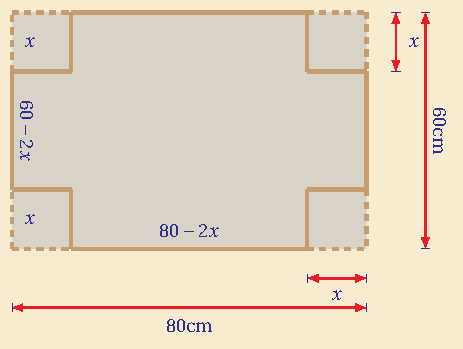
\includegraphics[scale=0.6]
{ejr-4-5-16.pdf}%
\caption{Ejemplo \ref{lacaja}}%
\label{lacaja2}%
\end{figure}
Supongamos que $x$ cent\'{\i}metros es la longitud de los cuadrados a
recortar. Las dimensiones, en $cm$, de la caja a construir son entonces:
\begin{align*}
\mbox{Largo:} &  80-2x\\
\mbox{Ancho:} &  60-2x\\
\mbox{Alto:} &  x
\end{align*}
Por lo que el volumen de la caja,en $cm^{3}$, expresado en funci\'{o}n de $x$
es:
\[
V(x)=x(80-2x)(60-2x)=2x(x-40)(x-30)=2x^{3}-140x^{2}+2400x
\]
donde el dominio \textquotedblleft pr\'{a}ctico" de la funci\'{o}n es $(0,30)$
(\textquestiondown Por qu\'{e}?). Si consideramos la funci\'{o}n en el cerrado
$[0,30]$, en el cual es continua, estamos interesados en el valor m\'{a}ximo
(positivo) de $V$. Es claro que tal m\'{a}ximo se alcanza en el abierto pues
en los extremos $V(x)=0$. Derivando tenemos
\[
V^{\prime}(x)=6x^{2}-280x+2400,
\]
de modo que la derivada es nula en
\begin{align*}
\frac{10}{3}\left(  7-\sqrt{13}\right)   &  \approx11.3148\\
\frac{10}{3}\left(  7+\sqrt{13}\right)   &  \approx35.3518
\end{align*}
de los cuales nos interesa solo $11.3148$, donde hay un m\'{a}ximo relativo.
Es para este valor aproximado que se alcanza el m\'{a}ximo volumen deseado.
\end{sol}

\begin{example}
De una l\'{a}mina circular de radio $R$ se recorta un sector circular, como el
de la f\'{\i}gura, para fabricar un cono circular recto. Determinar el
\'{a}ngulo $\theta$ para el cual el cono tenga un volumen m\'{a}ximo.%
\begin{center}
\includegraphics[scale=0.6]%
{ejr-4-5-17.pdf}%
\end{center}
\end{example}

\begin{sol}
El volumen del cono viene dado por
\begin{equation}
V=\frac{1}{3}\pi r^{2}h \label{Esc}%
\end{equation}
donde $r$ y $h$ son el radio y la altura del cono como se muestra en la
f\'{\i}gura. Note ademas que
\begin{align}
h  &  =\sqrt{R^{2}-r^{2}}\label{Esc1}\\
r  &  =\dfrac{R\theta}{2\pi}. \label{Esc2}%
\end{align}
De (\ref{Esc1}) en (\ref{Esc}) se tiene que:%
\begin{equation}
V=\frac{1}{3}\pi r^{2}\sqrt{R^{2}-r^{2}} \label{Esc3}%
\end{equation}
reemplazando finalmente (\ref{Esc2}) en (\ref{Esc3}), obtenemos $V=V\left(
\theta\right)  ,$ donde
\begin{align*}
V\left(  \theta\right)   &  =\frac{1}{3}\pi\left(  \dfrac{R\theta}{2\pi
}\right)  ^{2}\sqrt{R^{2}-\left(  \dfrac{R\theta}{2\pi}\right)  ^{2}}\\
V\left(  \theta\right)   &  =\frac{1}{24\pi^{2}}R^{3}\theta^{2}\sqrt{4\pi
^{2}-\theta^{2}}%
\end{align*}
Derivando $V\left(  \theta\right)  $ se obtiene:%
\[
\frac{dV\left(  \theta\right)  }{d\theta}=\frac{1}{24}R^{3}\theta\frac
{8\pi^{2}-3\theta^{2}}{\pi^{2}\sqrt{\left(  4\pi^{2}-\theta^{2}\right)  }}%
\]
Por lo tanto, los puntos cr\'{\i}ticos vienen dados por $\theta=0$ y
$\theta=\frac{2\pi}{3}\sqrt{6}$. Como $V\left(  \theta\right)  $ es continua
en $0\leq\theta\leq2\pi$, el teorema \ref{tvex} nos asegura la existencia de
un m\'{a}ximo y un m\'{\i}nimo para la funci\'{o}n en el intervalo. Para el
c\'{a}lculo de estos valores consideraremos la tabla siguiente
\[%
\begin{tabular}
[c]{|c|c|}\hline\hline
$x$ & $V\left(  \theta\right)  $\\\hline\hline
$0$ & $0$\\\hline
$\frac{2\pi}{3}\sqrt{6}$ & $V\left(  \frac{2\pi}{3}\sqrt{6}\right)  =\frac
{2}{27}\pi R^{3}\sqrt{3}$\\\hline
$2\pi$ & $0$\\\hline
\end{tabular}
\
\]
Entonces $V\left(  \theta\right)  $ toma su mayor valor cuando $\theta
=\frac{2\pi}{3}\sqrt{6}.$
\end{sol}

\begin{example}
Hallar las dimensiones del cilindro circular recto de m\'{a}ximo volumen que
puede incribirse en un cono circular recto de radio $R$ y altura $H.$
\end{example}

%

\begin{center}
\includegraphics[scale=0.6]%
{ejr-4-5-18.pdf}%
\end{center}
\begin{sol}
En la gr\'{a}fica se muestra una secci\'{o}n plana que contiene al eje del
cono. Sean $V$ el volumen, $h$ la altura y $r$ el radio de la base del
cilindro. El volumen $V$ en funci\'{o}n a la altura $h$ y el radio $r$ viene
dado por:%
\[
V=\pi r^{2}h\text{ },
\]


como el volumen est\'{a} en funci\'{o}n de las 2 variables, es necesario
encontrar una relaci\'{o}n entre $r$ y $h.$

Notese que $r\in\left[  0,R\right]  .$ En el caso que $r=0$ o $r=R$, se tiene
un cilindro ``degenerado'', es decir un cilindro con volumen nulo. Este mismo
resultado se puede obtener para $h\in\left[  0,H\right]  $ cuando $h=0$ y
$h=H.$

De la gr\'{a}fica de la derecha es clara la semejanza entre tri\'{a}ngulos que
permite obtener la relaci\'{o}n%
\[
\frac{H-h}{r}=\frac{H}{R}%
\]
de donde $h=-H\left(  \dfrac{r-R}{R}\right)  ,$ por lo cual
\begin{equation}
V\left(  r\right)  =-\pi r^{2}H\left(  \dfrac{r-R}{R}\right)  .
\label{vcilpco}%
\end{equation}
Derivando (\ref{vcilpco}) se tiene%
\[
V^{\prime}\left(  r\right)  =-\pi rH\frac{3r-2R}{R},
\]
por lo que los puntos cr\'{\i}ticos vienen dados por $r=0$ y $r=\frac{2}{3}R.$
Como $V\left(  r\right)  $ es continua en $\left[  0,R\right]  ,$el teorema
\ref{tvex} nos asegura la existencia de un m\'{a}ximo y un m\'{\i}nimo para la
funci\'{o}n$V$ en el intervalo. Para el c\'{a}lculo de estos valores
consideraremos la tabla siguiente
\[%
\begin{tabular}
[c]{|c|c|}\hline\hline
$r$ & $V\left(  r\right)  $\\\hline\hline
$0$ & $0$\\\hline
$\frac{2}{3}R$ & $\frac{4}{27}\pi R^{2}H$\\\hline
$R$ & $0$\\\hline
\end{tabular}
\ \
\]
Entonces $V\left(  r\right)  $ toma su mayor valor cuando $r=\frac{2}{3}R.$ Es
decir, las dimensiones del cilindro de mayor volumen que se puede incribir en
un cono de radio $R$ y altura $H$ viene dado por $r=\frac{2}{3}R$ y
$h=\frac{1}{3}H.$
\end{sol}

\section{Ejercicios propuestos}

\begin{center}
\textsc{I. Monoton\'{\i}a, Concavidad, m\'{a}ximos y m\'{\i}nimos.}
\end{center}

\begin{enumerate}
\item Determine (en caso de existir) para cada una de las funciones dadas a
continuaci\'{o}n : puntos cr\'{\i}ticos, m\'{a}ximos, m\'{\i}nimos, e
intervalos de monoton\'{\i}a.

\begin{enumerate}
\item $f\left(  x\right)  =x-\dfrac{24}{x+1}-5\ln\left(  x+1\right)  ^{2}.$

\item $f\left(  x\right)  =3x^{4}-44x^{3}+144x^{2}.$

\item $f\left(  x\right)  =x^{\frac{5}{3}}-5x^{\frac{2}{3}}.$

\item $f\left(  x\right)  =\dfrac{5x+16}{x+1}+2x.$

\item $f\left(  x\right)  =x^{3}-4x^{2}-6x+3.$

\item $f\left(  x\right)  =\left(  x^{2}-9\right)  ^{3}.$

\item $f\left(  x\right)  =\dfrac{9}{4\left(  2x+1\right)  }+\frac{9}{8}%
\ln\left(  2x+1\right)  ^{2}-\ln\left(  x+1\right)  ^{2}.$

\item $f\left(  x\right)  =xe^{\frac{-x^{2}}{8}}.$

\item $f\left(  x\right)  =x^{4}-3x^{3}+x^{2}-2.$
\end{enumerate}

\item Determine para cada una de las funciones a continuaci\'{o}n los valores
extremos en el intervalo cerrado dado.

\begin{enumerate}
\item $f\left(  x\right)  =x-\frac{24}{x+1}-5\ln\left(  x+1\right)  ^{2}$, en
$\left[  0,3\right]  .$

\item $f\left(  x\right)  =3x^{4}-44x^{3}+144x^{2}$, en $\left[  -3,4\right]
.$

\item $f\left(  x\right)  =\dfrac{5x+16}{x+1}+2x$, en $\left[  -\frac{1}%
{2},2\right]  .$

\item $f\left(  x\right)  =x^{3}-4x^{2}-6x+3$, en $\left[  -4,4\right]  .$

\item $f\left(  x\right)  =\left(  x^{2}-1\right)  ^{3}$, en $\left[
-2,1\right]  .$

\item $f\left(  x\right)  =\dfrac{9}{4\left(  2x+1\right)  }+\frac{9}{8}%
\ln\left(  2x+1\right)  ^{2}-\ln\left(  x+1\right)  ^{2}$, en $\left[
0,2\right]  .$

\item $f\left(  x\right)  =x^{3}e^{-\frac{x}{4}}$, en $\left[  -3,4\right]  .$

\item $f\left(  x\right)  =x+3\cos2x,$ en $\left[  0,\pi\right]  .$

\item $f\left(  x\right)  =e^{-\frac{1}{2}x}\left(  x^{2}+5x-2\right)  $ en
$\left[  -1,2\right]  .$
\end{enumerate}

\item Determine (en caso de existir) para cada una de las funciones dadas a
continuaci\'{o}n : puntos cr\'{\i}ticos, puntos de inflexi\'{o}n, m\'{a}ximos
y m\'{\i}nimos, intervalos de concavidad e intervalos de monoton\'{\i}a.

\begin{enumerate}
\item $f\left(  x\right)  =\dfrac{x}{2}+\cos x$, $x\in\left[  -\frac{3}{2}%
\pi,\frac{3}{2}\pi\right]  .$

\item $f\left(  x\right)  =xe^{-\frac{x^{2}}{2}}.$

\item $f\left(  x\right)  =\frac{3}{4}\left(  x^{2}-1\right)  ^{\frac{2}{3}}.$

\item $f\left(  x\right)  =5x^{\frac{2}{3}}-2x.$

\item $f\left(  x\right)  =1-9x-6x^{2}-x^{3}.$

\item $f\left(  x\right)  =2\cos x+\sin^{2}x,$ $x\in\left[  -2\pi,2\pi\right]
.$

\item $f\left(  x\right)  =\left(  x^{2}-4\right)  ^{3}.$

\item $f\left(  x\right)  =x^{2}e^{\frac{-x^{2}}{4}}.$

\item $f\left(  x\right)  =x\ln x^{2}.$

\item $f\left(  x\right)  =\frac{1}{4}x^{4}-\frac{7}{2}x^{2}+6x.$

\item $f\left(  x\right)  =e^{-\frac{1}{2}x}\left(  x^{2}+5x-2\right)  .$

\item $f\left(  x\right)  =\sqrt[3]{\left(  -x+1\right)  ^{2}}\left(
2x-1\right)  .$

\item $f\left(  x\right)  =-\dfrac{1}{\sqrt{2\pi}}e^{-\frac{x^{2}}{2}}.$

\item $f\left(  x\right)  =x^{3}e^{-x^{2}}.$
\end{enumerate}

\item Realice el bosquejo de la gr\'{a}fica de cada una de las funciones del
ejercicio 3.

Para las siguientes funciones determine

\begin{description}
\item[(i)] Intervalos de monoton\'{\i}a

\item[(ii)] Intervalos de Concavidad

\item[(iii)] Puntos cr\'{\i}ticos

\item[(iv)] Puntos de Inflexi\'{o}n

\item[(v)] Valores extremos

\item[(vi)] Dominio

\item[(vii)] Interceptos con los ejes

\item[(viii)] Asintotas
\end{description}

Construya con esta informaci\'{o}n la gr\'{a}fica de la funci\'{o}n citada y
comparela con la gr\'{a}fica dada

\begin{enumerate}
\item
$f\left(  x\right)  =\dfrac{x}{2}+\cos x,\! I=\left[  -\frac{3}{2}\pi,\frac
{3}{2}\pi\right]$  
\begin{center}
\includegraphics[scale=0.4]%
{ejp-4-6-4a.pdf}%
\end{center}
\item
$f\left(  x\right)  =xe^{-\frac{x^{2}}{2}}$
\begin{center}
%
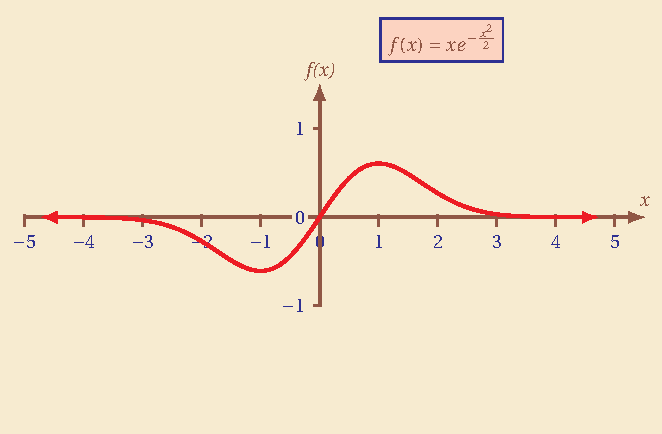
\includegraphics[scale=0.7]
{ejp-4-6-4b.pdf}%
\end{center}

\item
$f\left(  x\right)  =5x^{\frac{2}{3}}-2x$
\begin{center}
%
\includegraphics[scale=0.6]%
{ejp-4-6-4c.pdf}%
\end{center}

\item
$f\left(  x\right)  =1-9x-6x^{2}-x^{3}$
\begin{center}
%
\includegraphics[scale=0.6]%
{ejp-4-6-4d.pdf}%
\end{center}

\item
$f\left(  x\right)  =\left(  x\left(  8-x\right)  \right)  ^{\frac{2}{3}}$
\begin{center}
%
\includegraphics[scale=0.6]%
{ejp-4-6-4e.pdf}%
\end{center}

\item
$f\left(  x\right)  =2\cos x+\sin^{2}x,I=\left[  -2\pi,2\pi\right]  $
\begin{center}
%
\includegraphics[scale=0.6]%
{ejp-4-6-4f.pdf}%
\end{center}

\item
$f\left(  x\right)  =\left(  x^{2}-4\right)  ^{3}$
\begin{center}
%
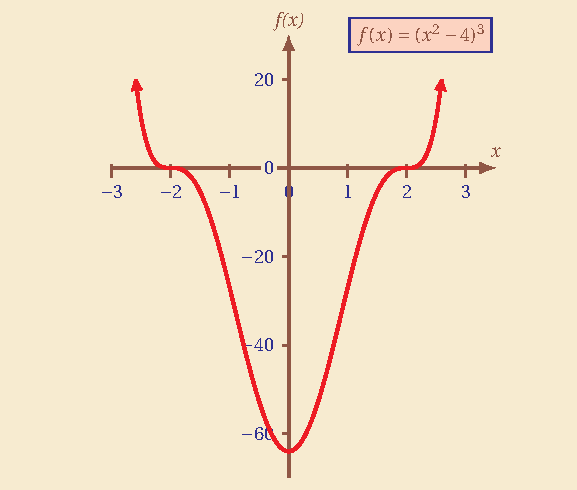
\includegraphics[scale=0.6]
{ejp-4-6-4g.pdf}%
\end{center}


\item
$f\left(  x\right)  =x^{2}e^{\frac{-x^{2}}{4}}$
\begin{center}
%
\includegraphics[scale=0.6]%
{ejp-4-6-4h.pdf}%
\end{center}

\item
$f\left(  x\right)  =x\ln x^{2}$
\begin{center}
%
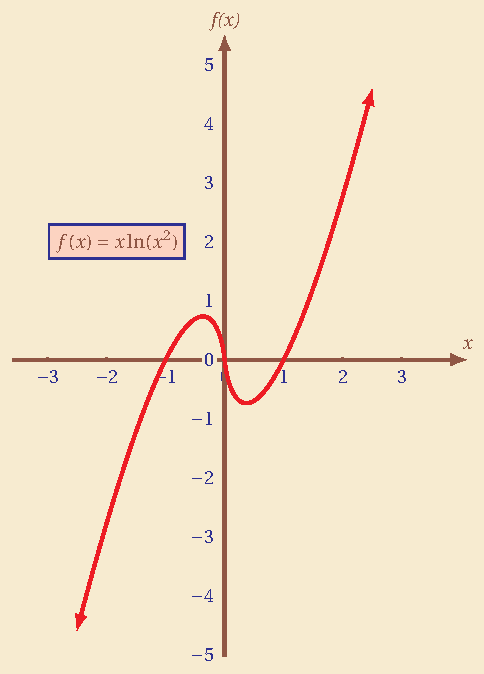
\includegraphics[scale=0.5]
{ejp-4-6-4i.pdf}%
\end{center}

\item  %TODO  
$f\left(  x\right)  =\frac{1}{4}x^{4}-\frac{7}{2}x^{2}+6x$
\begin{center}
%
\includegraphics[scale=0.5]%
{ejp-4-6-4j.pdf}
\end{center}%

\end{enumerate}

\item Sea
\[
g\left(  x\right)  =x^{3}+bx^{2}+cx+d
\]
Obtenga valores para $b,c$ y $d$ tal que se cumplan las siguientes tres condiciones:

\begin{itemize}
\item[i.] La grafica de la funci\'{o}n $g\left(  x\right)  $ contenga al punto
$A(2,2)$

\item[ii] $g\left(  x\right)  $ tenga un valor extremo en $x=4$

\item[ii.] $g\left(  x\right)  $ tenga un punto de inflexi\'{o}n en $x=2.$
\end{itemize}
\end{enumerate}

\begin{center}
\textsc{II. Razones relacionadas}
\end{center}

\begin{enumerate}
\item Si $2\operatorname{sen}x+4\tan y=3$ y $\dfrac{dy}{dt}=3,$ halle
$\dfrac{dx}{dt}$ en $\left(  \frac{1}{6}\pi,\frac{1}{3}\pi\right)  .$

\item Si $y\left(  \operatorname{sen}x+1\right)  =4$ y $\dfrac{dy}{dt}=-4,$
obtenga $\dfrac{dx}{dt}$ en $x=-\pi$

\item Si $s^{2}=x^{2}+y^{2}+3xy,s^{3}=7y^{2}-2x^{2}$ y $\dfrac{dy}{dt}=-2$.
Obtenga $\dfrac{ds}{dt}$ y $\dfrac{dx}{dt}$ cuando $\left(  x,y\right)
=\left(  1,1\right)  .$

\item Si $s^{2}=x\sin\theta,x^{2}+\cos^{2}\theta=2\theta,$ y $\dfrac
{dx}{d\theta}=\dfrac{1}{4}.$ Entonces calcule $\dfrac{ds}{d\theta}$ cuando
$\theta=\frac{\pi}{2}.$

\item Un punto $P$ se mueve, en sentido antihorario, sobre la circunferencia
$x^{2}+y^{2}=25.$ La distancia del punto a $\left(  -7,-7\right)  $ varia a
raz\'{o}n de $\frac{1}{2}$ unidad por segundo. Determine la raz\'{o}n a la
cual varian las coordenadas $x$ e $y$ cuando $\left(  x,y\right)  =\left(
-3,4\right)  .$

\item Un punto $P$ se mueve, en sentido horario, sobre la par\'{a}bola
$\left(  x-2\right)  ^{2}=-16\left(  y+5\right)  .$ La distancia del punto a
$\left(  0,-1\right)  $ varia a raz\'{o}n de $\frac{1}{3}$ unidad por segundo.
Determine la raz\'{o}n a la cual varian las coordenadas $x$ e $y$ cuando
$\left(  x,y\right)  =\left(  1,-\frac{81}{16}\right)  .$

\item \label{cap4prob7}Una v\'{\i}a de ferrocarril cruza una carretera
formandose un \'{a}ngulo de $60^{0}$, como lo muestra la figura$.$ Una
locomotora a $500$ metros de la intersecci\'{o}n se aleja de ella a raz\'{o}n
de $100\dfrac{km}{h}.$ Un automovil a $200$ metros de la intersecci\'{o}n se
acerca a ella a raz\'{o}n de $80\dfrac{km}{h}$ \textquestiondown Cu\'{a}l es
la variaci\'{o}n de la distancia entre la locomotora y el automovil?%

\begin{figure}[H]
\begin{center}
\includegraphics[scale=0.6]%
{ejp-4-6-7.pdf}%
\caption{Problema \ref{cap4prob7}.}%
\label{problematren}%
\end{center}
\end{figure}



\item \label{cap4prob8}Cierta cantidad de aceite fluye hacia el interior de un
deposito en forma de cono invertido a raz\'{o}n de $0.1\pi\,\frac{m^{3}}{\min
}.$ El deposito tiene un radio de 2.5 m en su parte superior y una profundidad
de 10 m. Si el deposito inicialmente tenia una peque\~{n}a cantidad de aceite,
\textquestiondown Qu\'{e} tan rapido cambia la altura del l\'{\i}quido, cuando
est\'{e} alcanza una altura de $8m$ en en interior del deposito?.%

\begin{figure}[H]
\centering
\includegraphics[scale=0.4]%
{ejp-4-6-8op.pdf}%
\caption{Problema \ref{cap4prob8}.}%
\label{figuraej8}%
\end{figure}


\item Una piedra es arrojada a un estanque tranquilo. Una serie de anillos
circulares conc\'{e}ntricos se extienden por el estanque y el radio de la
regi\'{o}n perturbada aumenta a raz\'{o}n de $4\dfrac{cm}{s}$.
\textquestiondown Con qu\'{e} rapidez aumenta dicha \'{a}rea cuando el radio
es de 4 cm?

\item Una escalera de 6 metros de longitud est\'{a} recargada sobre una rampa
que esta inclinada $60^{0}$ respecto de la horizontal. Si la base de la
escalera se esta resbalando a raz\'{o}n de $\frac{1}{20}\dfrac{m}{s},$
\textquestiondown Con qu\'{e} rapidez se desplazar\'{a} la parte superior de
la escalera cuando su base est\'{e} a 3 metros de la rampa?

\item Una antena de radar est\'{a} instalada en un barco situado a 7
kilometros de una costa recta, y gira a 32 rpm. \textquestiondown Con qu\'{e}
rapidez se desplaza el haz del radar a lo largo de la l\'{\i}nea costera
cuando dicho haz forma un \'{a}ngulo de $45^{0}$ con la citada l\'{\i}nea?

\item \label{cap4prob12}Un hombre de 1.80 m de estatura camina hacia un
edificio a una velocidad de $\frac{2}{3}\dfrac{m}{s}$. Si hay una luz en el
piso, que ilumina la fachada, localizada a 10 metros del edificio
\textquestiondown Con qu\'{e} rapidez se acorta la sombra de la persona
proyectada sobre la fachada cuando se encuentra a 4 metros de la
edificaci\'{o}n?.%

\begin{figure}[H]
\centering
\includegraphics[scale=2.5]%
{ejp-4-6-12.pdf}%
\caption{Problema \ref{cap4prob12}.}%
\label{ejemplo12}%
\end{figure}



\item Una escalera de $3m$ de largo resbala sobre una pared vertical. Si su
base se aleja de la pared a raz\'{o}n constante de $2m$ por segundo,
\textquestiondown a qu\'{e} velocidad resbala el extremo superior de la
escalera sobre la pared cuando la distancia de la base de la escalera a la
pared es de $1m$ ?

\item Una part\'{\i}cula m\'{o}vil se desplaza en el plano siguiendo una
trayectoria circular de ecuaci\'{o}n $x^{2}+y^{2}=1$. Si la abscisa cambia a
una raz\'{o}n de $2x$ unidades por segundo \textquestiondown c\'{o}mo
var\'{\i}a su ordenada cuando la part\'{\i}cula est\'{a} en el punto
$(\frac{1}{2},\frac{\sqrt{3}}{2})$?

\item El \'{a}rea de un cuadrado decrece a raz\'{o}n de $1.5cm^{2}$ por
segundo. Encuentre la raz\'{o}n de cambio de la longitud de los lados cuando
el \'{a}rea es de $100cm^{2}$. \textquestiondown C\'{o}mo est\'{a} cambiando,
en ese momento el \'{a}rea con relaci\'{o}n a la longitud de los lados?

\item Un bal\'{o}n esf\'{e}rico pierde volumen, sin perder su forma
esf\'{e}rica, a raz\'{o}n constante de $10\ cm^{3}$ por minuto.
\textquestiondown C\'{o}mo disminuye su radio? \textquestiondown Cu\'{a}l es
la raz\'{o}n de cambio del mismo cuando el volumen es de $60cm^{3}$?.

\item Un perro se encuentra entrenando sobre una pista par\'{a}bolica de
ecuaci\'{o}n
\[
y=3x^{2}-2x-2.
\]
Su amo se encuentra, en una caseta de observaci\'{o}n, en la posici\'{o}n
$\left(  2,10\right)  $ y quiere determinar si su perro puede seguir en las
carreras o se convierte en la mascota de sus hijos. La prueba consiste en
medir la rapidez vertical del perro en el punto final de la pista. La rapidez
vertical m\'{\i}nima exigida es de $1.3\frac{m}{s}.$ Si el recorrido se inicia
en la posici\'{o}n $\left(  -3,31\right)  $ y termina en la posici\'{o}n
$\left(  2,6\right)  $, y durante todo el recorrido la distancia a su
due\~{n}o tiene una variaci\'{o}n constante de $1.4\frac{m}{s}.$
\textquestiondown El perro pasa la prueba?.

\begin{center}
\includegraphics[scale=0.6]%
{ejp-4-6-17.pdf}%
\end{center}



\item Un deposito de agua con forma de prisma recto con secciones
transversales tri\'{a}ngulos is\'{o}sceles ,como el de la figura, es
alimentado por una manguera de la cual fluye agua a raz\'{o}n de
$1.8\frac{m^{3}}{\min}$. El deposito tambien presenta un escape del cual fluye
agua a raz\'{o}n de $0.22\frac{m^{3}}{\min}.$ \textquestiondown Qu\'{e} tan
rapido aumenta el nivel del agua (en $\frac{m}{\min}$),en el instante en que
la altura del agua es $2$ $m$?%
\begin{center}
\includegraphics[scale=0.4]%
{ejp-4-5-18op.pdf}%
\end{center}

\end{enumerate}

\begin{center}
\textsc{III. Optimizaci\'{o}n.}
\end{center}

\begin{enumerate}
\item Sea $\triangle ABC$ is\'{o}sceles con $AB=AC.$ Si $m\measuredangle
BAC=\alpha,$ obtenga el valor del \'{a}ngulo $\alpha$ tal que el \'{a}rea del
$\triangle ABC$ sea m\'{a}xima.

\item Determine dos n\'{u}meros positivos cuya suma sea $100$ y cuyo producto
sea m\'{a}ximo.

\item Una isla est\'{a} ubicada en el punto $A$, $4\,km$ mar adentro del punto
m\'{a}s cercano $B$ de una playa recta. Una atleta, en la isla desea ir al
punto $C$, a $6$ $km$ de $B$ playa abajo. La mujer puede dirigirse hacia el
punto $P$, entre $B$ y $C$, en un bote de remos a $3.5\dfrac{km}{h}$ y
desp\'{u}es caminar en forma recta de $P$ a $C$ a $6\dfrac{km}{h}.$
\textquestiondown Donde debe estar el punto $P$ (respecto a $B$) para que la
mujer se desplace en el menor tiempo posible?
\begin{center}
\includegraphics[scale=1]%
{ejp-4-6-3op.pdf}%
\end{center}

\item Determine el \'{a}rea del rect\'{a}ngulo m\'{a}s grande que tenga dos
v\'{e}rtices en el eje $x$ y los otros dos en la par\'{a}bola $y=16-x^{2},$
por arriba del eje $x.$

\item Determine la distancia m\'{\i}nima desde el punto $P\left(  1,0\right)
$ a un punto de la curva $y^{2}-x^{2}=9,$ y encuentre el punto de la curva
m\'{a}s cercano a $P.$

\item Pruebe que la distancia m\'{\i}nima desde el punto $P_{1}\left(
x_{1},y_{1}\right)  $ a la recta $l$ que tiene la ecuaci\'{o}n
\[
Ax+By+C=0
\]
esta dada por
\[
\dfrac{\left\vert Ax_{1}+By_{1}+C\right\vert }{\sqrt{A^{2}+B^{2}}}%
\]


\item Determine las dimensiones del cilindro con mayor volumen que pueda
inscribirse en un cono circular recto que tiene radio $R$ y altura $H.$

\item Un trozo de alambre de 80 centimetros de longitud se dobla en forma de
rect\'{a}ngulo. Determine las dimensiones del rect\'{a}ngulo de mayor \'{a}rea posible.

\item Una p\'{a}gina debe contener 150 centimetros cuadrados de material
impreso con 4 centimetros de margen superior e inferior y 2 centimetros de
margen derecho e izquierdo \textquestiondown Qu\'{e} dimensiones debe tener la
p\'{a}gina para que gaste menos papel?

\item Si se corta un alambre de 10 metros de longitud y se quiere formar un
rectangulo y una circunferencia \textquestiondown Donde debe cortarse el
alambre para que el \'{a}rea de las figuras combinadas sea m\'{a}xima.

\item Hay que construir una pileta de las dimensiones que se muestran.
S\'{o}lo se puede variar el \'{a}ngulo $\theta$ . \textquestiondown Con
qu\'{e} \'{a}ngulo se obtendr\'{a} el volumen m\'{a}ximo de la pileta?%
\begin{center}
\includegraphics[scale=0.4]%
{ejp-4-5-11op.pdf}%
\end{center}



\item Dos lados de un tri\'{a}ngulo tienen $a$ y $b$ de largo, y el \'{a}ngulo
entre ellos es $\theta.$ \textquestiondown Que valor de $\theta$
maximizar\'{a} el \'{a}rea del tri\'{a}ngulo?

\item Un granjero desea cercar tres terrenos rectangulares adyacentes
identicos, cada uno de ellos de 1800 pies cuadrados de \'{a}rea, incluyendo
cerca en medio de ellos. \textquestiondown Cu\'{a}les ser\'{\i}an las
dimensiones de los terrenos para emplear la menor cantidad de cerca posible?

\item Dada una esfera de radio $R$. Calcular en funci\'{o}n de $R$, el radio
$r$ y la altura $h$ del cono circular recto de mayor volumen que puede
inscribirse en la esfera.

\item Obtenga una ecuaci\'{o}n de la recta tangente a la curva
\[
y=\frac{1}{3}x^{3}+2x^{2}+5x-2
\]
cuya pendiente sea m\'{\i}nima

\item Si $a$ y $b$ son los catetos de un tri\'{a}ngulo rect\'{a}ngulo cuya
hipotenusa es $4$, hallar el mayor valor de $a^{2}+3b^{2}-5a+2.$

\item Dos f\'{a}bricas est\'{a}n situadas en las coordenadas $\left(
-3,0\right)  $ y $\left(  3,0\right)  $ y su central de suministro de
energ\'{\i}a en el punto $\left(  0,8\right)  .$ Determine donde debe
colocarse el punto $A$, tal que la longitud de conducci\'{o}n de la
energ\'{\i}a a las dos f\'{a}bricas sea m\'{\i}nima.%
\begin{center}
\includegraphics[scale=0.6]%
{ejp-4-6-17op.pdf}%
\end{center}


\item Una ventana tiene forma de rect\'{a}ngulo terminado por un semicirculo
de di\'{a}metro igual a la base del rect\'{a}ngulo. La parte circular ha de
ser de cristal transparente y la parte rectangular ha de ser de cristales de
color que admite solo dos tercios de la luz por metro cuadrado que el cristal
transparente. El perimetro total de la ventana ha de tener longitud fija $25$
m. Hallar las dimensiones de la ventana que deja pasar la mayor cantidad
posible de luz.

\item Hallar la menor distancia de $\left(  0,6\right)  $ del eje $Y$ a la
par\'{a}bola $x^{2}=4y.$

\item Considere la circunferencia de ecuaci\'{o}n
\[
x^{2}+y^{2}-2x+2y+1=0.
\]
Encuentre los puntos de la misma que est\'{a}n m\'{a}s cerca y m\'{a}s lejos
del origen del sistema de coordenadas.

\item Una caja cerrada de base cuadrada debe tener un volumen de $1000$
$cm^{3}.$ El material del fondo de la tapa de la caja tiene un costo de 0.3
euros por $cm^{2}$ y el material de los laterales cuesta $0.15$ euros por
$cm^{2}.$ Determine las dimensiones de la caja para que el costo total sea m\'{\i}nimo.

\item Se dobla la esquina superior izquierda de un trozo de papel de 8
pulgadas de ancho por 12 pulgadas de largo para llevarla hasta el borde de la
derecha, como en la figura. \textquestiondown Com\'{o} se doblar\'{\i}a de
modo que se minimice la longitud de doblez?. En otras palabras
\textquestiondown Como elegir\'{\i}a $x$ para minimizar $y$?%

\begin{center}
\includegraphics[scale=0.4]%
{pagina-doblada.pdf}%
\end{center}


\end{enumerate}



Ver� el resultado en la �ltima p�gina.
%%------------------------------------------------------------------------
%Cap�tulo Actualizaciones
%%------------------------------------------------------------------------
%\chapter{Actualizaciones}

%\figcontenido

\backmatter
%TCIDATA{LaTeXparent=0,0,Libropdf.tex}


\begin{thebibliography}{9999999999}                                                                                       %
\bibitem[\textbf{1}]{A}\textbf{Apostol, Tom.}\textquotedblleft Calculus". Vol
1. 2a. edici\'{o}n. Editorial Revert\'{e}.

\bibitem[\textbf{2}]{leh}\textbf{Lehmann, Charles.} \textquotedblleft
Algebra". M\'{e}xico. Limusa. 1981.

\bibitem[\textbf{3}]{Lei}\textbf{Leithold, Louis.} \textquotedblleft Algebra y
Trigonometr\'{\i}a con Geometr\'{\i}a anal\'{\i}tica". M\'{e}xico. Harla. 1994.

\bibitem[\textbf{4}]{Rudin}\textbf{Rudin, Walter.}\textquotedblleft Principles
of Mathematical Analysis". 3a. edici\'{o}n. MacGraw-Hill.

\bibitem[\textbf{5}]{S}\textbf{Spivak, Michael.}\textquotedblleft Calculus.
C\'{a}lculo infinitesimal". Volumen 1. Editorial Revert\'{e}.

\bibitem[\textbf{6}]{St}\textbf{Stewart, James.}\textquotedblleft C\'{a}lculo:
Conceptos y contextos". M\'{e}xico. Thomson.

\bibitem[\textbf{7}]{Swo}\textbf{Swokowski, Earl y Jeffrey Cole.}
\textquotedblleft Algebra y Trigonometr\'{\i}a con Geometr\'{\i}a
anal\'{\i}tica". 10a. edici\'{o}n. M\'{e}xico. Thomson.2002.

\bibitem[\textbf{8}]{Taylor}\textbf{Taylor, Howard y Thomas Wade}
\textquotedblleft\ Matem\'{a}ticas b\'{a}sicas ". M\'{e}xico. Limusa. 1975.

\bibitem[\textbf{9}]{Vance}\textbf{Vance, Elbridge.}\textquotedblleft\ Algebra
y Trigonometr\'{\i}a". 2a. edici\'{o}n. Fondo educativo Iberoamericano. 1978.

\bibitem[10]{Lang}\textbf{Lang, Serge. }An\'{a}lisis matem\'{a}tico.
Addison-Wesley. 1990.
\end{thebibliography}



\def\nbcolindex{2}
\pagecolor{mesh}
\printindex
\end{document}